%%%%
% June 4, 2015, CreateSpace ISBN created
% ISBN-13: 978-1514225158 
% 
% ISBN-10: 1514225158 
%%%%
\RequirePackage{ifthen}
\newboolean{longpage}
\setboolean{longpage}{false}
\ifthenelse{\boolean{longpage}}%
{\documentclass[10pt]{article}}%
{\documentclass[10pt]{book}}

\newboolean{printlabelname}
\setboolean{printlabelname}{false}
\ifthenelse{\boolean{printlabelname}}{\usepackage[notref,notcite]{showkeys}}{}
\usepackage{pdfpages}


%% end detour
%\usepackage{amsmath}
\usepackage{xr}
\externaldocument{Calculus}

\input{headers/Page_Size_Calculus}
\usepackage{APEX_format}
\input{headers/Header_Calculus}
\usepackage{pgfplots}
\pgfplotsset{compat=1.8}
\usepackage{pdfpages}



\ifthenelse{\boolean{xetex}}%
	{\sffamily
	%%\usepackage{fontspec}
	\usepackage{mathspec}
	\setallmainfonts[Mapping=tex-text]{Calibri}
	\setmainfont[Mapping=tex-text]{Calibri}
	\setsansfont[Mapping=tex-text]{Calibri}
	\setmathsfont(Greek){[cmmi10]}}
	{}
	
	\ifthenelse{\boolean{luatex}}%
	{\sffamily
	\usepackage{fontspec}
	\usepackage{unicode-math}
	%\usepackage{mathspec}
	%\setallmainfonts[Mapping=tex-text]{Calibri}
	\setmainfont{Calibri}
	%\setsansfont[Mapping=tex-text]{Calibri}
	\setmathfont[range=\mathup]{Calibri}
	\setmathfont[range=\mathit]{Calibri Italic}
	}
	{}

\makeindex

%%%\tracingonline=1
\begin{document}
%\printexercisenames
%\printincolor
\printinblackandwhite
\usetwoDgraphics
\printallanswers


\input{text/front_matter_and_coverII}


%\chapter{Limits}\label{chapter:limits}
%\thispagestyle{empty}

%\textit{Calculus} means ``a method of calculation or reasoning.'' When one computes the sales tax on a purchase, one employs a simple calculus. When one finds the area of a polygonal shape by breaking it up into a set of triangles, one is using another calculus. Proving a theorem in geometry employs yet another calculus.

Despite the wonderful advances in mathematics that had taken place into the first half of the $17^\text{th}$ century, mathematicians and scientists were keenly aware of what they \textit{could not do.} (This is true even today.) In particular, two important concepts eluded mastery by the great thinkers of that time: area and rates of change. 

Area seems innocuous enough; areas of circles, rectangles, parallelograms, etc., are standard topics of study for students today just as they were then. However, the areas of \textit{arbitrary} shapes could not be computed, even if the boundary of the shape could be described exactly. 

Rates of change were also important. When an object moves at a constant rate of change, then ``distance = rate $\times $ time.'' But what if the rate is not constant -- can distance still be computed? Or, if distance is known, can we discover the rate of change?

It turns out that these two concepts were related. Two mathematicians, Sir Isaac Newton and Gottfried Leibniz, are credited with independently formulating a system of computing that solved the above problems and showed how they were connected. Their system of reasoning was ``a'' calculus. However, as the power and importance of their discovery took hold, it became known to many as ``the'' calculus. Today, we generally shorten this to discuss ``calculus.''

The foundation of ``the calculus'' is the \textit{limit.} It is a tool to describe a particular behavior of a function. This chapter begins our study of the limit by approximating its value graphically and numerically. After a formal definition of the limit, properties are established that make ``finding limits'' tractable. Once the limit is understood, then the problems of area and rates of change can be approached.



\section{An Introduction To Limits}\label{sec:limit_intro}

We begin our study of \textit{limits} by considering examples that demonstrate key concepts that will be explained as we progress.\\

Consider the function $y = \frac{\sin x}{x}$. When $x$ is near the value 1, what value (if any) is $y$ near?%

While our question is not precisely formed (what constitutes ``near the value 1''?), the answer does not seem difficult to find. One might think first to look at a graph of this function to approximate the appropriate $y$ values. Consider Figure \ref{fig:zoom_sinx_over_x}, where $y = \frac{\sin x}{x}$ is graphed. For values of $x$ near 1, it seems that $y$ takes on values near $0.85$. In fact, when $x=1$, then $y=\frac{\sin 1}{1} \approx 0.84$, so it makes sense that when $x$ is ``near'' 1, $y$ will be ``near'' $0.84$.

\mfigure{.8}{$\sin(x)/x$ near $x=1$.}{fig:zoom_sinx_over_x}{figures/figZoomSinXOverX}
\mfigure{.55}{$\sin(x)/x$ near $x=0$.}{fig:sinx_over_x}{figures/figSinXOverX}
Consider this again at a different value for $x$. When $x$ is near 0, what value (if any) is $y$ near? By considering Figure \ref{fig:sinx_over_x}, one can see that it seems that $y$ takes on values near $1$. But what happens when $x=0$? We have $$ y \rightarrow \frac{\sin 0}{0} \rightarrow \raisebox{8pt}{\text{``\ }}\frac{0}{0}\raisebox{8pt}{\text{\ ''}}.$$ 
The expression ``$0/0$'' has no value; it is \emph{indeterminate.} \index{limit!indeterminate form}\index{indeterminate form} Such an expression gives no information about what is going on with the function nearby. We cannot find out how $y$ behaves near $x=0$ for this function simply by letting $x=0$. 

\emph{Finding a limit} entails understanding how a function behaves near a particular value of $x$. Before continuing, it will be useful to establish some notation. Let $y=f(x)$; that is, let $y$ be a function of $x$ for some function $f$. The expression ``the limit of $y$ as $x$ approaches 1'' describes a number, often referred to as $L$, that $y$ nears as $x$ nears 1. We write all this as $$\lim_{x\to 1} y = \lim_{x\to 1} f(x) = L.$$ This is not a complete definition (that will come in the next section); this is a pseudo-definition that will allow us to explore the idea of a limit. \index{limit!pseudo-definition}

Above, where $f(x) = \sin(x)/x$, we approximated $$\lim_{x\to 1} \frac{\sin x}{x} \approx 0.84 \quad \text{ and } \quad \lim_{x\to 0}\frac{\sin x}{x} \approx 1.$$ (We \textit{approximated} these limits, hence used the ``$\approx$'' symbol, since we are working with the pseudo-definition of a limit, not the actual definition.)

Once we have the true definition of a limit, we will find limits \textit{analytically}; that is, exactly using a variety of mathematical tools. For now, we will \textit{approximate} limits both graphically and numerically. Graphing a function can provide a good approximation, though often not very precise. Numerical methods can provide a more accurate approximation. We have already approximated limits graphically, so we now turn our attention to numerical approximations.


Consider again $\lim_{x\to 1}\sin (x)/x$. To approximate this limit numerically, we can create a table of $x$ and $f(x)$ values where $x$ is ``near'' 1. This is done in Figure \ref{table:sinx_1}.\par

Notice that for values of $x$ near $1$, we have $\sin (x)/x$ near $0.841$. The $x=1$ row is in bold to highlight the fact that when considering limits, we are \textit{not} concerned with the value of the function at that particular $x$ value; we are only concerned with the values of the function when $x$ is \textit{near} 1. 

\mtable{.3}{Values of $\sin(x)/x$ with $x$ near 1.}{table:sinx_1}{\input{figures/sinx_over_x_table_1}}

%\vskip \baselineskip

Now approximate $\lim_{x\to 0} \sin(x)/x$ numerically. We already approximated the value of this limit as 1 graphically in Figure \ref{fig:sinx_over_x}. The table in Figure \ref{table:sinx_2} shows the value of $\sin(x)/x$ for values of $x$ near 0. Ten places after the decimal point are shown to highlight how close to 1 the value of $\sin(x)/x$ gets as $x$ takes on values very near 0. We include the $x=0$ row in bold again to stress that we are not concerned with the value of our function at $x=0$, only on the behavior of the function \textit{near} 0. 

\mtable{.8}{Values of $\sin(x)/x$ with $x$ near 0.}{table:sinx_2}{\input{figures/sinx_over_x_table_2}}
 
This numerical method gives confidence to say that 1 is a good approximation of $\lim_{x\to 0} \sin(x)/x$; that is, $$\lim_{x\to 0} \sin(x)/x \approx 1.$$ Later we will be able to prove that the limit is \textit{exactly} 1.

We now consider several examples that allow us explore different aspects of the limit concept.\\

\mfigure{.55}{Graphically approximating a limit in Example \ref{ex_limit1}.}{fig:limit1}{figures/figlimit1}
\mtable{.35}{Numerically approximating a limit in Example \ref{ex_limit1}.}{table:limit1}{\input{figures/table_limit1}}

\example{ex_limit1}{Approximating the value of a limit}{
Use graphical and numerical methods to approximate $$\lim_{x\to 3} \frac{x^2-x-6}{6x^2-19x+3}.$$}%
{To graphically approximate the limit, graph $$y = (x^2-x-6)/(6x^2-19x+3)$$ on a small interval that contains 3. To numerically approximate the limit, create a table of values where the $x$ values are near 3. This is done in Figures \ref{fig:limit1} and \ref{table:limit1}, respectively.

\enlargethispage{2\baselineskip}

The graph shows that when $x$ is near 3, the value of $y$ is very near $0.3$. By considering values of $x$ near 3, we see that $y=0.294$ is a better approximation. The graph and the table imply that $$\lim_{x\to 3} \frac{x^2-x-6}{6x^2-19x+3} \approx 0.294.$$ 
\vskip -\baselineskip
}\\

This example may bring up a few questions about approximating limits (and the nature of limits themselves). 
\begin{enumerate}
\item		If a graph does not produce as good an approximation as a table, why bother with it?
\item		How many values of $x$ in a table are ``enough?'' In the previous example, could we have just used $x=3.001$ and found a fine approximation?
\end{enumerate}

Graphs are useful since they give a visual understanding concerning the behavior of a function. Sometimes a function may act ``erratically'' near certain $x$ values which is hard to discern numerically but very plain graphically. Since graphing utilities are very accessible, it makes sense to make proper use of them.


Since tables and graphs are used only to \textit{approximate} the value of a limit, there is not a firm answer to how many data points are ``enough.'' Include enough so that a trend is clear, and use values (when possible) both less than and greater than the value in question. In Example \ref{ex_limit1}, we used both values less than and greater than 3. Had we used just $x=3.001$, we might have been tempted to conclude that the limit had a value of $0.3$. While this is not far off, we could do better. Using values ``on both sides of 3'' helps us identify trends.\\

\example{ex_limit2}{Approximating the value of a limit}{
Graphically and numerically approximate the limit of $f(x)$ as $x$ approaches 0, where $$f(x) = \left\{\begin{array}{rl} x+1 & x< 0 \\ -x^2+1 & x > 0 \end{array}\right..$$}{Again we graph $f(x)$ and create a table of its values near $x=0$ to approximate the limit. Note that this is a piecewise defined function, so it behaves differently on either side of 0. Figure \ref{fig:limit2} shows a graph of $f(x)$, and on either side of 0 it seems the $y$ values approach 1. Note that $f(0)$ is not actually defined, as indicated in the graph with the open circle.

\mfigure{.65}{Graphically approximating a limit in Example \ref{ex_limit2}.}{fig:limit2}{figures/figlimit2}
\mtable{.45}{Numerically approximating a limit in Example \ref{ex_limit2}.}{table:limit2}{\input{figures/table_limit2}}

The table shown in Figure \ref{table:limit2} shows values of $f(x)$ for values of $x$ near 0. It is clear that as $x$ takes on values very near 0, $f(x)$ takes on values very near 1. It turns out that if we let $x=0$ for either ``piece'' of $f(x)$, 1 is returned; this is significant and we'll return to this idea later.

The graph and table allow us to say that $\lim_{x\to 0}f(x) \approx 1$; in fact, we are probably very sure it \emph{equals} 1.
}\\

\enlargethispage{\baselineskip}
\vskip \baselineskip
\noindent\textbf{\large Identifying When Limits Do Not Exist}\\

A function may not have a limit for all values of $x$. That is, we cannot say $\lim_{x\to c}f(x)=L$ for some numbers $L$ for all values of $c$, for there may not be a number that $f(x)$ is approaching. There are three common ways in which a limit may fail to exist. \index{limit!does not exist}
\begin{enumerate}
\item		The function $f(x)$ may approach different values on either side of $c$.
\item		The function may grow without upper or lower bound as $x$ approaches $c$.
\item		The function may oscillate as $x$ approaches $c$ without approaching a specific value.
\end{enumerate}

We'll explore each of these in turn.\\

\vskip \baselineskip

%\noindent
%

\example{ex_no_limit1}{Different Values Approached From Left and Right}{
Explore why $\ds\lim_{x\to 1} f(x)$ does not exist, where $$f(x) = \left\{\begin{array}{cl} x^2-2x+3 & x\leq 1 \\ x & x>1 \end{array}\right..$$}%
{
A graph of $f(x)$ around $x=1$ and a table are given in Figures \ref{fig:nolimit1} and \ref{table:nolimit1}, respectively. It is clear that as $x$ approaches 1, $f(x)$ does not seem to approach a single number. Instead, it seems as though $f(x)$ approaches two different numbers. When considering values of $x$ less than 1 (approaching 1 from the left), it seems that $f(x)$ is approaching 2; when considering values of $x$ greater than 1 (approaching 1 from the right), it seems that $f(x)$ is approaching 1. Recognizing this behavior is important; we'll study this in greater depth later. Right now, it suffices to say that the limit does not exist since $f(x)$ is not approaching one value as $x$ approaches 1.
\mfigure{.8}{Observing no limit as $x\to 1$ in Example \ref{ex_no_limit1}.}{fig:nolimit1}{figures/fignolimit1}
\mtable{.6}{Values of $f(x)$ near $x=1$ in Example \ref{ex_no_limit1}.}{table:nolimit1}{\input{figures/table_nolimit1}}
}\\

%
%\vskip \baselineskip
%\noindent\textbf{The Function Grows Without Bound}\\

%\input{figures/fig_nolimit2}
\example{ex_no_limit2}{The Function Grows Without Bound}{
Explore why $\ds\lim_{x\to 1} 1/(x-1)^2$ does not exist.}%
{A graph and table of $f(x) = 1/(x-1)^2$ are given in Figures \ref{fig:nolimit2} and \ref{table:nolimit2}, respectively. Both show that as $x$ approaches 1, $f(x)$ grows larger and larger. 
\mfigure{.4}{Observing no limit as $x\to 1$ in Example \ref{ex_no_limit2}.}{fig:nolimit2}{figures/fignolimit2}
\mtable{.2}{Values of $f(x)$ near $x=1$ in Example \ref{ex_no_limit2}.}{table:nolimit2}{\input{figures/table_nolimit2}}

We can deduce this on our own, without the aid of the graph and table. If $x$ is near 1, then $(x-1)^2$ is very small, and: $$\frac{1}{\text{very small number}} = \text{very large number}.$$
Since $f(x)$ is not approaching a single number, we conclude that $$\lim_{x\to 1}\frac{1}{(x-1)^2}$$ does not exist.
}\\

%\vskip \baselineskip
%\noindent\textbf{The Function Oscillates}\\

\example{ex_no_limit3}{The Function Oscillates}{
Explore why $\ds\lim_{x\to 0}\sin(1/x)$ does not exist.}%
{%\mfigure{.4}{Observing no limit as $x\to 0$ in Example \ref{ex_no_limit3}.}{fig:nolimit3a}{figures/figNoLimit3a}
%\mfigure{.2}{Zooming in to observing no limit as $x\to 0$ in Example \ref{ex_no_limit3}.}{fig:nolimit3b}{figures/figNoLimit3b}
Two graphs of $f(x) = \sin(1/x)$ are given in Figures \ref{fig:nolimit3}. Figure \ref{fig:nolimit3}(a) shows $f(x)$ on the interval $[-1,1]$; notice how $f(x)$ seems to oscillate near $x=0$. One might think that despite the oscillation, as $x$ approaches 0, $f(x)$ approaches 0. However, Figure \ref{fig:nolimit3}(b) zooms in on $\sin(1/x)$, on the interval $[-0.1,0.1]$. Here the oscillation is even more pronounced. Finally, in the table in Figure \ref{fig:nolimit3}(c), we see $\sin(1/x)$ evaluated for values of $x$ near 0. As $x$ approaches 0, $f(x)$ does not appear to approach any value. 

It can be shown that in reality, as $x$ approaches 0, $\sin(1/x)$ takes on all values between $-1$ and 1 infinitely many times! Because of this oscillation,

 $\ds\lim_{x\to 0}\sin(1/x)$ does not exist.}\\

\ifthenelse{\boolean{longpage}}%%% if longpage, squeeze it in
{\vskip\baselineskip
\noindent\begin{minipage}{\textwidth}\centering
\begin{tabular}{cc}
(a) \myincludegraphics[scale=.9]{figures/figNoLimit3a} & (b) \myincludegraphics[scale=.9]{figures/figNoLimit3b}\end{tabular}
\vskip \baselineskip
\begin{tabular}{c}
(c)\begin{tabular}[b]{cc}
 $x$ & $\sin(1/x)$ \\ \hline 0.1 & $-0.544021$ \\ 0.01 & $-0.506366$ \\ 0.001 & 0.82688 \\ 0.0001 & $-0.305614$ \\ $1.\times 10^{-5}$ & 0.0357488 \\
 $1.\times 10^{-6}$ & $-0.349994$ \\ $1.\times 10^{-7}$ & 0.420548 \\ \\\end{tabular}\end{tabular}%
\captionsetup{type=figure}%
\caption{Observing that $f(x) = \sin(1/x)$ has no limit as $x\to 0$ in Example \ref{ex_no_limit3}.}\label{fig:nolimit3}
\end{minipage}} %% else, not longpage

%\vskip 1\baselineskip
\ifthenelse{\isodd{\thepage}}{}{\noindent\hskip -\marginparwidth }
\noindent\begin{minipage}{\textwidth+\marginparwidth+\marginparsep}%\centering
\begin{tabular}{ccc}
\myincludegraphics{figures/figNoLimit3a} &  \myincludegraphics{figures/figNoLimit3b} &  \begin{tabular}[b]{cc}
 $x$ & $\sin(1/x)$ \\ \hline 0.1 & $-0.544021$ \\ 0.01 & $-0.506366$ \\ 0.001 & 0.82688 \\ 0.0001 & $-0.305614$ \\ $1.\times 10^{-5}$ & 0.0357488 \\
 $1.\times 10^{-6}$ & $-0.349994$ \\ $1.\times 10^{-7}$ & 0.420548 \\ \\\end{tabular}\\
(a) & (b) & (c)\end{tabular}%
\captionsetup{type=figure}%
\caption{Observing that $f(x) = \sin(1/x)$ has no limit as $x\to 0$ in Example \ref{ex_no_limit3}.}\label{fig:nolimit3}
\end{minipage}
}
\vskip 2\baselineskip

%\vskip \baselineskip
\noindent\textbf{\large Limits of Difference Quotients}\\

We have approximated limits of functions as $x$ approached a particular number. We will consider another important kind of limit after explaining a few key ideas.\index{limit!difference quotient}

\mfigure{.35}{Interpreting a difference quotient as the slope of a secant line.}{fig:diffquot1}{figures/figDiffQuot1}

Let $f(x)$ represent the position function, in feet, of some particle that is moving in a straight line, where $x$ is measured in seconds. Let's say that when $x=1$, the particle is at position 10 ft., and when $x=5$, the particle is at 20 ft. Another way of expressing this is to say $$f(1)=10 \quad \text{ and } \quad f(5) = 20.$$
Since the particle traveled 10 feet in 4 seconds, we can say the particle's \textit{average velocity} was 2.5 ft/s. We write this calculation using a ``quotient of differences,'' or, a \textit{difference quotient}: $$\frac{f(5) - f(1)}{5-1} = \frac{10}4 = 2.5 \text{ft/s}.$$

This difference quotient can be thought of as the familiar ``rise over run'' used to compute the slopes of lines. In fact, that is essentially what we are doing: given two points on the graph of $f$, we are finding the slope of the \textit{secant line} through those two points. See Figure \ref{fig:diffquot1}.

Now consider finding the average speed on another time interval. We again start at $x=1$, but consider the position of the particle $h$ seconds later. That is, consider the positions of the particle when $x=1$ and when $x=1+h$. The difference quotient is now $$\frac{f(1+h)-f(1)}{(1+h)-1} = \frac{f(1+h)-f(1)}h.$$

Let $f(x) = -1.5x^2+11.5x$; note that $f(1)=10$ and $f(5) = 20$, as in our discussion. We can compute this difference quotient for all values of $h$ (even negative values!) except $h=0$, for then we get ``0/0,'' the indeterminate form introduced earlier. For all values $h\neq 0$, the difference quotient computes the average velocity of the particle over an interval of time of length $h$ starting at $x=1$. 

For small values of $h$, i.e., values of $h$ close to 0, we get average velocities over very short time periods and compute secant lines over small intervals. See Figure \ref{fig:diff_quot_small_h}. This leads us to wonder what the limit of the difference quotient is as $h$ approaches 0. That is, $$\lim_{h\to 0} \frac{f(1+h)-f(1)}{h} = \text{ ? }$$

\vskip \baselineskip
\ifthenelse{\boolean{longpage}}% in longpage form
			{% is longpage
			\noindent\begin{minipage}{\textwidth}\centering
			\begin{tabular}{cc}
			(a) \myincludegraphics{figures/figDiffQuotSmallha} & (b) \myincludegraphics{figures/figDiffQuotSmallhb}%
			\end{tabular}
			\begin{tabular}{c} (c)\myincludegraphics{figures/figDiffQuotSmallhc}\end{tabular}
			\captionsetup{type=figure}%
			\caption{Secant lines of $f(x)$ at $x=1$ and $x=1+h$, for shrinking values of $h$ (i.e., $h\rightarrow 0$).}\label{fig:diff_quot_small_h}
			\end{minipage}
			\vskip 2\baselineskip
			}% end longpage
			{% isn't longpage
%			\ifthenelse{\isodd{\thepage}}{}{\noindent\hskip -\marginparwidth \hskip -\marginparsep}
%			\noindent\begin{minipage}{\textwidth+\marginparwidth+\marginparsep}%\centering
			\mtable{.61}{Secant lines of $f(x)$ at $x=1$ and $x=1+h$, for shrinking values of $h$ (i.e., $h\rightarrow 0$).}{fig:diff_quot_small_h}{\begin{tabular}{c}
			\myincludegraphics{figures/figDiffQuotSmallha}\\ (a)\\ \myincludegraphics{figures/figDiffQuotSmallhb} 
			\\ (b)\\ \myincludegraphics{figures/figDiffQuotSmallhc}\\(c)\end{tabular}%
			}
%			\captionsetup{type=figure}%
%			\caption{Secant lines of $f(x)$ at $x=1$ and $x=1+h$, for shrinking values of $h$ (i.e., $h\rightarrow 0$).}\label{fig:diff_quot_small_h}
%			\end{minipage}
%			\vskip 2\baselineskip
			}% ends isn't a longpage

As we do not yet have a true definition of a limit nor an exact method for computing it, we settle for approximating the value. While we could graph the difference quotient (where the $x$-axis would represent $h$ values and the $y$-axis would represent values of the difference quotient) we settle for making a table. See Figure \ref{table:diff_quot_smallh}. The table gives us reason to assume the value of the limit is about 8.5. \\

%\ifthenelse{\boolean{longpage}}{\mtable{.3}{The difference quotient evaluated at values of $h$ near 0.}{table:diff_quot_smallh}{\begin{tabular}{cc}$h$ & $\frac{f(1+h)-f(1)}{h}$\vspace{1pt} \\ \hline $-0.5$ & 9.25 \\ $-0.1$ & 8.65 \\ $-0.01$ & 8.515 \\ 0.01 & 8.485 \\ 0.1 & 8.35 \\ 0.5 & 7.75 \end{tabular}} }
%{}

%\vskip \baselineskip
\enlargethispage{\baselineskip}

Proper understanding of limits is key to understanding calculus. With limits, we can accomplish seemingly impossible mathematical things, like adding up an infinite number of numbers (and not get infinity) and finding the slope of a line between two points, where the ``two points'' are actually the same point. These are not just mathematical curiosities; they allow us to link position, velocity and acceleration together, connect cross-sectional areas to volume, find the work done by a variable force, and much more.

\ifthenelse{\boolean{longpage}}{}{\mtable{.2}{The difference quotient evaluated at values of $h$ near 0.}{table:diff_quot_smallh}{\begin{tabular}{cc}$h$ & $\frac{f(1+h)-f(1)}{h}$\vspace{1pt} \\ \hline $-0.5$ & 9.25 \\ $-0.1$ & 8.65 \\ $-0.01$ & 8.515 \\ 0.01 & 8.485 \\ 0.1 & 8.35 \\ 0.5 & 7.75 \end{tabular}} }

In the next section we give the formal definition of the limit and begin our study of finding limits analytically. In the following exercises, we continue our introduction and approximate the value of limits.\\

\printexercises{exercises/01_01_exercises}

%\clearpage

%\input{text/01_Limit_Definition}
%\input{text/01_Analytic_Limits}
%\section{One Sided Limits}\label{sec:limit_continuity}

%\noindent\hskip-50pt\hskip-45pt\parbox{45pt}{\textbf{\itshape Review:}}
%\begin{minipage}[t]{\textwidth+50pt}
%We introduced the concept of a limit gently, approximating their values graphically and numerically. Next came the rigorous definition of the limit, along with an admittedly tedious method for computing them. The previous section gave us tools (which we call theorems) that allow us to compute limits with greater ease. Chief among the results were the facts that polynomials and rational, trigonometric, exponential and logarithmic functions (and their sums, products, etc.) all behave ``nicely.'' In this section we rigorously define what we mean by ``nicely.''
%\end{minipage}\\
%
%\vskip \baselineskip

We introduced the concept of a limit gently, approximating their values graphically and numerically. Next came the rigorous definition of the limit, along with an admittedly tedious method for evaluating them. The previous section gave us tools (which we call theorems) that allow us to compute limits with greater ease. Chief among the results were the facts that polynomials and rational, trigonometric, exponential and logarithmic functions (and their sums, products, etc.) all behave ``nicely.'' In this section we rigorously define what we mean by ``nicely.''

In Section \ref{sec:limit_intro} we saw three ways in which limits of functions failed to exist: 
	\begin{enumerate}
	\item	The function approached different values from the left and right,
	\item	The function grows without bound, and 
	\item	The function oscillates.
	\end{enumerate}
	
In this section we explore in depth the concepts behind \#1 by introducing the \textit{one-sided limit}. We begin with formal definitions that are very similar to the definition of the limit given in Section \ref{sec:limit_def}, but the notation is slightly different and ``$x\neq c$'' is replaced with either ``$x<c$'' or ``$x>c$.''
%\small

%
%\ifthenelse{\boolean{longpage}}{}
%{\setlength{\specialboxlength}{\textwidth+4\specialboxinnerseplength}}
\enlargethispage{3\baselineskip}
%\setboxwidth{115pt}%
%\noindent\ifthenelse{\isodd{\thepage}}{}{\hskip -115pt}%
%\noindent\begin{minipage}{\specialboxlength}
\definition{def:onesidedlimit}{One Sided Limits: Left- and Right-Hand Limits}
{%
\textbf{Left-Hand Limit} \index{limit!one sided}\index{limit!right handed}\index{limit!left handed}

\indent Let $f$ be a function defined on $(a,c)$ for some $a<c$ and let $L$ be a real number. 

The \sword{limit of $f(x)$, as $x$ approaches $c$ from the left, is $L$}, or, \sword{the left-hand limit of $f$ at $c$ is $L$}, denoted by  
$$\displaystyle \lim_{x\rightarrow c^-} f(x) = L,$$
means  given any $\epsilon > 0$, there exists $\delta > 0$ such that for all $a<x<c$,  
if  $|x - c| < \delta$, then $|f(x) - L| < \epsilon$.\\

% Version 3.0 definition
%\textbf{Left-Hand Limit} \index{limit!one sided}\index{limit!right handed}\index{limit!left handed}
%%
%%\indent Let $I$ be an open interval containing $c$, and let $f$ be a function defined on $I$, except possibly at $c$. 
%%The \sword{limit of $f(x)$, as $x$ approaches $c$ from the left, is $L$}, or, \sword{the left--hand limit of $f$ at $c$ is $L$}, denoted by  
%%$$\displaystyle \lim_{x\rightarrow c^-} f(x) = L,$$
%%means that given any $\epsilon > 0$, there exists $\delta > 0$ such that for all $x< c$,  
%%if  $|x - c| < \delta$, then $|f(x) - L| < \epsilon$.\\
%%% Really old definition
% Let $f$ be a function defined on an open interval containing $c$. 
%%%The notation $$ \lim_{x\rightarrow c^-} f(x) = L, $$ read as ``the limit of $f(x)$ as $x$ approaches $c$ from the left is $L$,'' or ``the \textit{left-hand limit of $f$ at $c$ is L}'' 
%%%means that given any $\epsilon > 0$, there exists $\delta > 0$ such that 
%%%$|x - c| < \delta$ implies $|f(x) - L| < \epsilon$, for all $x<c$.\\

\textbf{Right-Hand Limit}

\indent Let $f$ be a function defined on $(c,b)$ for some $b>c$ and let $L$ be a real number. 

The \sword{limit of $f(x)$, as $x$ approaches $c$ from the right, is $L$}, or, \sword{the right-hand limit of $f$ at $c$ is $L$}, denoted by  
$$\displaystyle \lim_{x\rightarrow c^+} f(x) = L,$$
means  given any $\epsilon > 0$, there exists $\delta > 0$ such that for all $c<x<b$,  
if  $|x - c| < \delta$, then $|f(x) - L| < \epsilon$.
%Version 3.0 Definition
%Let $I$ be an open interval containing $c$, and let $f$ be a function defined on $I$, except possibly at $c$. 
%The \sword{limit of $f(x)$, as $x$ approaches $c$ from the right, is $L$}, or, \sword{the right--hand limit of $f$ at $c$ is $L$}, denoted by  
%$$\displaystyle \lim_{x\rightarrow c^+} f(x) = L,$$
%means that given any $\epsilon > 0$, there exists $\delta > 0$ such that for all $x> c$,  
%if  $|x - c| < \delta$, then $|f(x) - L| < \epsilon$.
%%% Really old definition
%%% Let $f$ be a function defined on an open interval containing $c$. The notation $$ \lim_{x\rightarrow c^+} f(x) = L, $$ read as ``the limit of $f(x)$ as $x$ approaches $c$ from the right is $L$,'' or ``the \textit{right-hand limit of $f$ at $c$ is L}'' 
%%means that given any $\epsilon > 0$, there exists $\delta > 0$ such that 
%%$|x - c| < \delta$ implies $|f(x) - L| < \epsilon$, for all $x>c$.
}
%\end{minipage}
\restoreboxwidth
\normalsize

Practically speaking, when evaluating a left-hand limit, we consider only values of $x$ ``to the left of $c$,'' i.e., where $x<c$. The admittedly imperfect notation $x\to c^-$ is used to imply that we look at values of $x$ to the left of $c$. The notation has nothing to do with positive or negative values of either $x$ or $c$. A similar statement holds for evaluating right-hand limits; there we consider only values of $x$ to the right of $c$, i.e., $x>c$. We can use the theorems from previous sections to help us evaluate these limits; we just restrict our view to one side of $c$.

We practice evaluating left- and right-hand limits through a series of examples.\\

\example{ex_onesidea}{Evaluating one sided limits}{
Let $\ds f(x) = \left\{\begin{array}{cc} x & 0\leq x\leq 1 \\ 3-x & 1<x<2\end{array},\right.$ as shown in Figure \ref{fig:onesided1}. Find each of the following: 

\noindent\begin{minipage}[t]{.5\textwidth}
\begin{enumerate}
\item		$\ds \lim_{x\to 1^-} f(x)$
\item		$\ds \lim_{x\to 1^+} f(x)$
\item		$\ds \lim_{x\to 1} f(x)$
\item		$\ds f(1)$
\end{enumerate}
\end{minipage}
\begin{minipage}[t]{.5\textwidth}
\begin{enumerate}\addtocounter{enumi}{4}
\item		$\ds \lim_{x\to 0^+} f(x)$
\item		$f(0)$
\item		$\ds \lim_{x\to 2^-} f(x)$
\item		$f(2)$
\end{enumerate}
\end{minipage}

\mfigure{.65}{A graph of $f$ in Example \ref{ex_onesidea}.}{fig:onesided1}{figures/figOneSidedLimits1}
}
{For these problems, the visual aid of the graph is likely more effective in evaluating the limits than using $f$ itself. Therefore we will refer often to the graph.
			\begin{enumerate}
			\item		As $x$ goes to 1 \textit{from the left}, we see that $f(x)$ is approaching the value of 1. Therefore $\ds \lim_{x\to 1^-} f(x) =1.$
			\item		As $x$ goes to 1 \textit{from the right}, we see that $f(x)$ is approaching the value of 2. Recall that it does not matter that there is an ``open circle'' there; we are evaluating a limit, not the value of the function. Therefore $\ds \lim_{x\to 1^+} f(x)=2$.
			\item		\textit{The} limit of $f$ as $x$ approaches 1 does not exist, as discussed in the first section. The function does not approach one particular value, but two different values from the left and the right.
			\item		Using the definition and by looking at the graph we see that $f(1) = 1$.
			\item		As $x$ goes to 0 from the right, we see that $f(x)$ is also approaching 0. Therefore $\ds \lim_{x\to 0^+} f(x)=0$. Note we cannot consider a left-hand limit at 0 as $f$ is not defined for values of $x<0$.
			\item		Using the definition and the graph, $f(0) = 0$.
			\item		As $x$ goes to 2 from the left, we see that $f(x)$ is approaching the value of 1. Therefore $\ds \lim_{x\to 2^-} f(x)=1.$
			\item		The graph and the definition of the function show that $f(2)$ is not defined.
			\end{enumerate}
\vskip -\baselineskip
}\\

Note how the left and right-hand limits were different at $x=1$. This, of course, causes \textit{the} limit to not exist. The following theorem states what is fairly intuitive: \textit{the} limit exists precisely when the left and right-hand limits are equal.

\theorem{thm:leftrightlimits}{Limits and One Sided Limits}
{Let $f$ be a function defined on an open interval $I$ containing $c$. \index{limit!does not exist} Then $$\lim_{x\to c}f(x) = L$$ if, and only if, $$\lim_{x\to c^-}f(x) = L \quad \text{and} \quad \lim_{x\to c^+}f(x) = L.$$}

The phrase ``if, and only if'' means the two statements are \textit{equivalent}: they are either both true or both false. If the limit equals $L$, then the left and right hand limits both equal $L$. If the limit is not equal to $L$, then at least one of the left and right-hand limits is not equal to $L$ (it may not even exist).
			
One thing to consider in Examples \ref{ex_onesidea} -- \ref{ex_onesided} is that the value of the function may/may not be equal to the value(s) of its left/right-hand limits, even when these limits agree. \\

\example{ex_onesideb}{Evaluating limits of a piecewise--defined function}{
Let $f(x) = \left\{\begin{array}{cc} 2-x & 0<x<1 \\ (x-2)^2 & 1<x<2 \end{array}.\right.$  Evaluate the following. 

\noindent\begin{minipage}[t]{.5\textwidth}
		\begin{enumerate}
		\item		$\ds \lim_{x\to 1^-} f(x)$
		\item		$\ds \lim_{x\to 1^+} f(x)$
		\item		$\ds \lim_{x\to 1} f(x)$
		\item		$\ds f(1)$
		\end{enumerate}
		\end{minipage}
		\begin{minipage}[t]{.5\textwidth}
		\begin{enumerate}\addtocounter{enumi}{4}
		\item		$\ds \lim_{x\to 0^+} f(x)$
		\item		$f(0)$
		\item		$\ds \lim_{x\to 2^-} f(x)$
		\item		$f(2)$
		\end{enumerate}	
		\end{minipage}
		
}
{In this example, we evaluate each expression using just the definition of $f$, without using a graph as we did in the previous example.
		\begin{enumerate}
		\item		As $x$ approaches 1 from the left, we consider a limit where all $x$-values are less than 1. This means we use the $2-x$ piece of the piecewise function $f$ as the domain for that piece is $(0,1)$. As the $x$-values near 1, $2-x$ approaches 1; that is, $f(x)$ approaches 1. Therefore $\ds \lim_{x\to 1^-} f(x)=1.$
		\item		As $x$ approaches 1 from the right, we consider a limit where all $x$-values are greater than 1. This means we use the $(x-2)^2$ piece of $f$ as the domain for that piece is $(1,2)$. As the $x$-values near 1, $(x-2)^2$ approaches 1; that is, we see that again $f(x)$ approaches 1. Therefore $\ds \lim_{x\to 1+} f(x)=1$.
		\item		\textit{The} limit of $f$ as $x$ approaches 1 exists and is 1, as $f$ approaches 1 from both the right and left. Therefore $\ds \lim_{x\to 1} f(x)=1$.
		\item		Neither piece of $f$ is defined for the $x$-value of 1; in other words, 1 is not in the domain of $f$. Therefore $f(1)$ is not defined.  %Note that 1 is not in the domain of $f$ as defined by the problem, which is indicated on the graph by an open circle when $x=1$.
		\item		As $x$ approaches  0 from the right, we consider a limit where all $x$-values are greater than 0. This means we use the $2-x$ piece of $f$. As the $x$-values near 0, $2-x$ approaches 2; that is, $f(x)$ approaches 2. So $\ds \lim_{x\to 0^+} f(x)=2$.
		\item		$f(0)$  is not defined as $0$ is not in the domain of $f$.
		\item		As $x$ approaches  2 from the left, we consider a limit where all $x$-values are less than 2. This means we use the $(x-2)^2$ piece of $f$. As the $x$-values near 2, $(x-2)^2$ nears 0; that is, $f(x)$ approaches 0. So $\ds \lim_{x\to 2^-} f(x)=0$.
		\item		$f(2)$  is not defined as 2 is not in the domain of $f$.
		\end{enumerate}
We can confirm our analytic result by consulting the graph of $f$ shown in Figure \ref{fig:onesidedb}.	Note the open circles on the graph at $x=0$, $1$ and $2$, where $f$ is not defined.	
		\mfigure{.8}{A graph of $f$ from Example \ref{ex_onesideb}}{fig:onesidedb}{figures/figOneSidedLimits2}
%\vskip -\baselineskip
}\\

\example{ex_onesidec}{Evaluating limits of a piecewise--defined function}{
Let $f(x) = \left\{\begin{array}{cc} (x-1)^2 & 0\leq x\leq 2, x\neq 1\\ 1 & x=1\end{array},\right.$ as shown in Figure \ref{fig:onesidedc}. Evaluate the following.

		\noindent\begin{minipage}[t]{.5\textwidth}
		\begin{enumerate}
		\item		$\ds \lim_{x\to 1^-} f(x)$
		\item		$\ds \lim_{x\to 1^+} f(x)$
		\end{enumerate}
		\end{minipage}
		\begin{minipage}[t]{.5\textwidth}
		\begin{enumerate}\addtocounter{enumi}{2}
		\item		$\ds \lim_{x\to 1} f(x)$
		\item		$f(1)$
		\end{enumerate}
		\end{minipage}
		
\mfigure{.30}{Graphing $f$ in Example \ref{ex_onesidec}}{fig:onesidedc}{figures/figOneSidedLimits3}		
}
{		It is clear by looking at the graph that both the left and right-hand limits of $f$, as $x$ approaches 1, are 0. Thus it is also clear that \textit{the} limit is 0; i.e., $\ds \lim_{x\to 1} f(x) = 0$. It is also clearly stated that $f(1) = 1$. \vskip .4\baselineskip
}\\

%\vskip .5\baselineskip

\example{ex_onesided}{Evaluating limits of a piecewise--defined function}{
Let $f(x) = \left\{\begin{array}{cc} x^2 & 0\leq x\leq 1 \\ 2-x & 1<x\leq 2\end{array},\right.$ as shown in Figure \ref{fig:onesidedd}. Evaluate the following. 

		\noindent\begin{minipage}[t]{.5\textwidth}
		\begin{enumerate}
		\item		$\ds \lim_{x\to 1^-} f(x)$
		\item		$\ds \lim_{x\to 1^+} f(x)$
		\end{enumerate}
		\end{minipage}
				\noindent\begin{minipage}[t]{.5\textwidth}
		\begin{enumerate}\addtocounter{enumi}{2}
		\item		$\ds \lim_{x\to 1} f(x)$
		\item		$f(1)$
		\end{enumerate}
		\end{minipage}
		
}
{		It is clear from the definition of the function and its graph that all of the following are equal:
\mfigure{.8}{Graphing $f$ in Example \ref{ex_onesided}}{fig:onesidedd}{figures/figOneSidedLimits4}
$$ \lim_{x\to 1^-} f(x) = \lim_{x\to 1^+} f(x) =\lim_{x\to 1} f(x) =f(1) = 1.$$
}\\

In Examples \ref{ex_onesidea} -- \ref{ex_onesided} we were asked to find both $\ds \lim_{x\to 1}f(x)$ and $f(1)$. Consider the following table:
\begin{center}
\begin{tabular}{ccc} & $\ds \lim_{x\to 1}f(x)$ & $f(1)$ \vspace{2pt}\\ \hline
Example \ref{ex_onesidea} & does not exist & 1 \\
Example \ref{ex_onesideb} & 1 & not defined \\
Example \ref{ex_onesidec} & 0 & 1 \\
Example \ref{ex_onesided} & 1 & 1 \\
\end{tabular}
\end{center}

Only in Example \ref{ex_onesided} do both the function and the limit exist and agree. This seems ``nice;'' in fact, it seems ``normal.'' This is in fact an important situation which we explore in the next section, entitled ``Continuity.'' In short, a \textit{continuous function} is one in which when a function approaches a value as $x\rightarrow c$ (i.e., when $\ds \lim_{x\to c} f(x) = L$), it actually \textit{attains} that value at $c$. Such functions behave nicely as they are very predictable.

\printexercises{exercises/01_04_exercises}
%\input{text/01_Continuity}
%\input{text/01_Limits_Involving_Infinity}
%

%%\addtocounter{chapter}{1}

%\clearpage{\pagestyle{empty}\cleardoublepage}
%\chapter{Derivatives}\label{chapter:derivatives}
%\thispagestyle{empty}
%\addtocontents{toc}{\protect\enlargethispage{4\baselineskip}}
%
%\input{text/02_Derivative}
%\input{text/02_Derivative_Meaning}
%\section{Basic Differentiation Rules}\label{sec:basic_diff_rules}

The derivative is a powerful tool but is admittedly awkward given its reliance on limits. Fortunately, one thing mathematicians are good at is \textit{abstraction.} For instance, instead of continually finding derivatives at a point, we abstracted and found the derivative function. 

Let's practice abstraction on linear functions, $y=mx+b$. What is $y\primeskip'$? Without limits, recognize that linear functions are characterized by being functions with a constant rate of change (the slope). The derivative, $y\primeskip'$, gives the instantaneous rate of change; with a linear function, this is constant, $m$. Thus $y\primeskip'=m$. 

Let's abstract once more. Let's find the derivative of the general quadratic function, $f(x) = ax^2+bx+c$. Using the definition of the derivative, we have:
		\begin{align*}
		\fp(x) 	&=	\lim_{h\to 0}\frac{a(x+h)^2+b(x+h)+c-(ax^2+bx+c)}{h} \\
						&=	\lim_{h\to 0} \frac{ah^2+2ahx+bh}{h} \\
						&=	\lim_{h\to 0} ah+2ax+b\\
						&= 2ax+b.
		\end{align*}
		
So if $y = 6x^2+11x-13$, we can immediately compute $y\primeskip' = 12x+11$. \\

In this section (and in some sections to follow) we will learn some of what mathematicians have already discovered about the derivatives of certain functions and how derivatives interact with arithmetic operations. We start with a theorem.

%\setboxwidth{110pt}
%\noindent\hskip-110pt
%\begin{minipage}{\specialboxlength}
\theorem{thm:deriv_common}{Derivatives of Common Functions}{
		\noindent\begin{minipage}[t]{.6\linewidth}
		\begin{enumerate}
		\item		\sword{Constant Rule:}\index{derivative!Constant Rule} 
		
		$\ds \frac{d}{dx}\big( c\big) = 0$, where $c$ is a constant.
		
		\item		\sword{Power Rule:}\index{derivative!Power Rule}\index{Power Rule!differentiation}
		
		$\ds \frac{d}{dx}\big(x^n\big) = nx^{n-1}$, \parbox[t]{60pt}{where $n$ is an integer, $n>0$.}
		
		
		
		\end{enumerate}
		\end{minipage}
		\begin{minipage}[t]{.39\linewidth}
		\begin{enumerate}\addtocounter{enumi}{4}
		 
		\item		$\ds \frac{d}{dx}(\sin x) = \cos x$
		
		\item		$\ds \frac{d}{dx}(\cos x) = -\sin x$
		
		\item		$\ds \frac{d}{dx}\left(e^x\right) = e^x$
		
		\item		$\ds \frac{d}{dx}(\ln x) = \frac{1}{x}$
		\end{enumerate}\index{derivative!basic rules}
		\end{minipage}
}
%\end{minipage}
%\restoreboxwidth

%\setboxwidth{110pt}
%\noindent\hskip-110pt
%\begin{minipage}{\specialboxlength}
%\theorem{thm:deriv_common}{Derivatives of Common Functions}{
		%\noindent\begin{minipage}[t]{175pt}
		%\begin{enumerate}
		%\item		\sword{Constant Rule:}\index{derivative!Constant Rule} 
		%
		%$\ds \frac{d}{dx}\big( c\big) = 0$, where $c$ is a constant.\addtocounter{enumi}{1}
		%\item		$\ds \frac{d}{dx}(\sin x) = \cos x$\addtocounter{enumi}{1}
		%\item		$\ds \frac{d}{dx}\left(e^x\right) = e^x$
		%\end{enumerate}
		%\end{minipage}
		%\begin{minipage}[t]{210pt}
		%\begin{enumerate}\addtocounter{enumi}{1}
		%\item		\sword{Power Rule:}\index{derivative!Power Rule}\index{Power Rule!differentiation}
		%
		%$\ds \frac{d}{dx}\left(x^n\right) = nx^{n-1}$, where $n$ is an integer, $n>0$.\addtocounter{enumi}{1}
		%\item		$\ds \frac{d}{dx}(\cos x) = -\sin x$\addtocounter{enumi}{1}
		%\item		$\ds \frac{d}{dx}(\ln x) = \frac{1}{x}$
		%\end{enumerate}\index{derivative!basic rules}
		%\end{minipage}
%}
%\end{minipage}
%\restoreboxwidth

This theorem starts by stating an intuitive fact: constant functions have no rate of change as they are \textit{constant}. Therefore their derivative is 0 (they change at the rate of 0). The theorem then states some fairly amazing things. The Power Rule states that the derivatives of Power Functions (of the form $y=x^n$) are very straightforward: multiply by the power, then subtract 1 from the power. We see something incredible about the function $y=e^x$: it is its own derivative. We also see a new connection between the sine and cosine functions. 

One special case of the Power Rule is when $n=1$, i.e., when $f(x) = x$. What is $\fp(x)$? According to the Power Rule, $$\fp(x) = \frac{d}{dx}\big(x\big) = \frac{d}{dx}\big(x^1\big) = 1\cdot x^0 = 1.$$ In words, we are asking ``At what rate does $f$ change with respect to $x$?'' Since $f$ \textit{is} $x$, we are asking ``At what rate does $x$ change with respect to $x$?'' The answer is: 1. They change at the same rate.\\

\enlargethispage{1\baselineskip}
Let's practice using this theorem.\\

\example{ex_deriv_rule1}{Using Theorem \ref{thm:deriv_common} to find, and use, derivatives}
{Let $f(x)=x^3$. 

		%\noindent\begin{minipage}[t]{.5\textwidth}
		\begin{enumerate}
		\item		Find $\fp(x)$.
		\item		Find the equation of the line tangent to the graph of $f$ at $x=-1$. 
%		\end{enumerate}
%		\end{minipage}
%		\begin{minipage}[t]{.5\textwidth}
%		\begin{enumerate}
		\item		Use the tangent line to approximate $(-1.1)^3$.
		\item		Sketch $f$, $\fp$ and the found tangent line on the same axis.
		\end{enumerate}
%		\end{minipage}
}
{	\begin{enumerate}
\enlargethispage{\baselineskip}
		\item		The Power Rule states that if $f(x) = x^3$, then $\fp(x) = 3x^2$. 

		\item		To find the equation of the line tangent to the graph of $f$ at $x=-1$, we need a point and the slope. The point is $(-1,f(-1)) = (-1, -1)$. The slope is $\fp(-1)= 3$. Thus the tangent line has equation $y = 3(x-(-1))+(-1) = 3x+2$. 
		
		\item		We can use the tangent line to approximate $(-1.1)^3$ as $-1.1$ is close to $-1$. We have $$(-1.1)^3 \approx 3(-1.1)+2 = -1.3.$$
			We can easily find the actual answer; $(-1.1)^3 = -1.331$. 
		
		\item		See Figure \ref{fig:xcubedwithderiv}.
		\mfigure{.5}{A graph of $f(x) = x^3$, along with its derivative $\fp(x) = 3x^2$ and its tangent line at $x=-1$.}{fig:xcubedwithderiv}{figures/figxcubedwithderiv}
		\end{enumerate}
\vskip-1.5\baselineskip
}\\
\clearpage

Theorem \ref{thm:deriv_common} gives useful information, but we will need much more. For instance, using the theorem, we can easily find the derivative of $y=x^3$, but it does not tell how to compute the derivative of $y=2x^3$, $y=x^3+\sin x$ nor $y=x^3\sin x$. The following theorem helps with the first two of these examples (the third is answered in the next section).
\enlargethispage{\baselineskip}

\theorem{thm:deriv_prop}{Properties of the Derivative}
{Let $f$ and $g$ be differentiable on an open interval $I$ and let $c$ be a real number. Then:
	\begin{enumerate}
	%\item		\parbox{75pt}{\textbf{Sum/Difference Rule:}}\parbox[t]{176pt}{$\ds \frac{d}{dx}\Big(f(x) \pm g(x)\Big) = \frac{d}{dx}\Big(f(x)\Big) \pm \frac{d}{dx}\Big(g(x)\Big)$ $= \rule{0pt}{15pt}\fp(x)\pm g\primeskip'(x)$}
	\item	\sword{Sum/Difference Rule:}
	
	$\ds \frac{d}{dx}\Big(f(x) \pm g(x)\Big) = \frac{d}{dx}\Big(f(x)\Big) \pm \frac{d}{dx}\Big(g(x)\Big)$ $= \rule{0pt}{15pt}\fp(x)\pm g\primeskip'(x)$
	\index{derivative!Sum/Difference Rule}\index{Sum/Difference Rule!of derivatives}
	\item		\sword{Constant Multiple Rule:}
	
	$\ds \frac{d}{dx}\Big(c\cdot f(x)\Big) = c\cdot\frac{d}{dx}\Big(f(x)\Big) = c\cdot\fp(x)$.\index{derivative!Constant Multiple Rule}\index{Constant Multiple Rule!of derivatives}
	\end{enumerate}
}

Theorem \ref{thm:deriv_prop} allows us to find the derivatives of a wide variety of functions. It can be used in conjunction with the Power Rule to find the derivatives of any polynomial. Recall in Example \ref{ex_deriv1} that we found, using the limit definition, the derivative of $f(x) = 3x^2+5x-7$. We can now find its derivative without expressly using limits:
		\begin{align*}
		\frac{d}{dx}\Big(3x^2+5x+7\Big) &= 3\frac{d}{dx}\Big(x^2\Big) + 5\frac{d}{dx}\Big(x\Big) + \frac{d}{dx}\Big(7\Big) \\
																		&= 3\cdot 2x+5\cdot 1+ 0\\
																		&= 6x+5.
		\end{align*}

We were a bit pedantic here, showing every step. Normally we would do all the arithmetic and steps in our head and readily find $\ds \frac{d}{dx}\Big(3x^2+5x+7\Big) = 6x+5.$\\

\example{ex_der2}{Using the tangent line to approximate a function value}{
Let $f(x) = \sin x + 2x+1$. Approximate $f(3)$ using an appropriate tangent line.}
{This problem is intentionally ambiguous; we are to \textit{approximate} using an \textit{appropriate} tangent line. How good of an approximation are we seeking? What does appropriate mean?

In the ``real world,'' people solving problems deal with these issues all time. One must make a judgment using whatever seems reasonable. In this example, the actual answer is $f(3) = \sin 3 + 7$, where the real problem spot is $\sin 3$. What is $\sin 3$?

Since $3$ is close to $\pi$, we can assume $\sin 3\approx \sin \pi = 0$. Thus one guess is $f(3) \approx 7$. Can we do better? Let's use a tangent line as instructed and examine the results; it seems best to find the tangent line at $x=\pi$. 

Using Theorem \ref{thm:deriv_common} we find $\fp(x) = \cos x + 2$. The slope of the tangent line is thus $\fp(\pi) = \cos \pi + 2 =1$. Also, $f(\pi) = 2\pi+1 \approx 7.28$. So the tangent line to the graph of $f$ at $x=\pi$ is $y=1(x-\pi)+ 2\pi+1 =x+\pi+1 \approx x+4.14$. Evaluated at $x=3$, our tangent line gives $y=3+4.14 = 7.14$. Using the tangent line, our final approximation is that $f(3) \approx 7.14$.

Using a calculator, we get an answer accurate to 4 places after the decimal: $f(3) = 7.1411$. Our initial guess was $7$; our tangent line approximation was more accurate, at $7.14$.

The point is \textit{not} ``Here's a cool way to do some math without a calculator.'' Sure, that might be handy sometime, but your phone could probably give you the answer. Rather, the point is to say that tangent lines are a good way of approximating, and many scientists, engineers and mathematicians often face problems too hard to solve directly. So they approximate.
}\\

%\enlargethispage{2\baselineskip}
%\vskip \baselineskip
\noindent\textbf{\large Higher Order Derivatives}\\

\mnote{.4}{\textbf{Note:} The second derivative notation could be written as $$\frac{d\primeskip^2y}{dx^2}=\frac{d\primeskip^2y}{(dx)^2}=\frac{d\primeskip^2}{(dx)^2}\big(y\big).$$ That is, we take the derivative of $y$ twice (hence $d\primeskip^2$), both times with respect to $x$ (hence $(dx)^2=dx^2$).}
The derivative of a function $f$ is itself a function, therefore we can take its derivative. The following definition gives a name to this concept and introduces its notation.
\enlargethispage{2\baselineskip}
%\clearpage
%\small
\definition{def:Higher_Deriv}{Higher Order Derivatives}
{Let $y=f(x)$ be a differentiable function on $I$. The following are defined, provided the corresponding limits exist. \index{derivative!higher order}\index{derivative!notation}\index{derivative!second}\index{derivative!third}
		\begin{enumerate}
		\item		The \sword{second derivative of $f$} is: 
						$$ \fp'(x) = \frac{d}{dx}\Big(\fp(x)\Big) = \frac{d}{dx}\left(\frac{dy}{dx}\right) = \frac{d\primeskip^2y}{dx^2}=y\primeskip''.$$
				\item		The \sword{third derivative of $f$} is: 
						$$ \fp''(x) = \frac{d}{dx}\Big(\fp'(x)\Big) = \frac{d}{dx}\left(\frac{d\primeskip^2y}{dx^2}\right) = \frac{d\primeskip^3y}{dx^3}=y\primeskip'''.$$
				\item		The \sword{n$^{\text{th}}$ derivative of $f$} is:
						$$ f\,^{(n)}(x) = \frac{d}{dx}\left(f\,^{(n-1)}(x)\right) = \frac{d}{dx}\left(\frac{d\primeskip^{n-1}y}{dx^{n-1}}\right) = \frac{d\primeskip^ny}{dx^n}=y^{(n)}.$$
		\end{enumerate}
}
\normalsize

In general, when finding the fourth derivative and on, we resort to the $f\,^{(4)}(x)$ notation, not $\fp'''(x)$; after a while, too many ticks is  confusing.\\

Let's practice using this new concept.\\

\example{ex_high_order}{Finding higher order derivatives}{
Find the first four derivatives of the following functions:
	
	
	\noindent\begin{minipage}[t]{.5\textwidth}
	\begin{enumerate}
	\item		$f(x) = 4x^2$
	\item		$f(x) = \sin x$
	\end{enumerate}
	\end{minipage}
	\noindent\begin{minipage}[t]{.5\textwidth}
	\begin{enumerate}\addtocounter{enumi}{2}
	\item		$f(x) = 5e^x$
	\end{enumerate}
	\end{minipage}
}
{\begin{enumerate}
	\item		Using the Power and Constant Multiple Rules, we have: $\fp(x) = 8x$. Continuing on, we have 
	$$\fp'(x) = \frac{d}{dx}\big(8x\big) = 8;\qquad \fp''(x) = 0;\qquad f\,^{(4)}(x) = 0.$$ Notice how all successive derivatives will also be 0.
	\item		We employ Theorem \ref{thm:deriv_common} repeatedly.
	$$\fp(x) = \cos x;\qquad \fp'(x) = -\sin x;\qquad \fp''(x) = -\cos x;\qquad f\,^{(4)}(x) = \sin x.$$ Note how we have come right back to $f(x)$ again. (Can you quickly figure what $f\,^{(23)}(x)$ is?)
	\item		Employing Theorem \ref{thm:deriv_common} and the Constant Multiple Rule, we can see that $$\fp(x) = \fp'(x) = \fp''(x) = f\,^{(4)}(x) = 5e^x.$$
	\end{enumerate}
\vskip-1.5\baselineskip
}
\vskip \baselineskip
\noindent\textbf{\large Interpreting Higher Order Derivatives}\\

What do higher order derivatives \textit{mean}? What is the practical interpretation? \index{derivative!higher order!interpretation}

Our first answer is a bit wordy, but is technically correct and beneficial to understand. That is,
	\begin{quote}
	The second derivative of a function $f$ is the rate of change of the rate of change of $f$.
	\end{quote}

One way to grasp this concept is to let $f$ describe a position function. Then, as stated in Key Idea \ref{idea:motion}, $\fp$ describes the rate of position change: velocity. We now consider $\fp'$, which describes the rate of velocity change. Sports car enthusiasts talk of how fast a car can go from 0 to 60 mph; they are bragging about the \textit{acceleration} of the car.

We started this chapter with amusement--park riders free--falling with position function $f(t) = -16t^2+150$. It is easy to compute $\fp(t)=-32t$ ft/s and $\fp'(t) = -32$ (ft/s)/s. We may recognize this latter constant; it is the acceleration due to gravity. In keeping with the unit notation introduced in the previous section, we say the units are ``feet per second per second.'' This is usually shortened to ``feet per second squared,'' written as ``ft/s$^2$.''

It can be difficult to consider the meaning of the third, and higher order, derivatives. The third derivative is ``the rate of change of the rate of change of the rate of change of $f$.'' That is essentially meaningless to the uninitiated. In the context of our position/velocity/acceleration example, the third derivative is the ``rate of change of acceleration,'' commonly referred to as ``jerk.'' 

Make no mistake: higher order derivatives have great importance even if their practical interpretations are hard (or ``impossible'') to understand. The mathematical topic of \textit{series} makes extensive use of higher order derivatives.

\printexercises{exercises/02_03_exercises}
%\input{text/02_Product_Quotient_Rules}
%\input{text/02_Chain_Rule}
%\input{text/02_Implicit_Differentiation}
%\input{text/02_Derivative_Inverse_Functions}
%
%\addtocounter{chapter}{2}
%
%\clearpage{\pagestyle{empty}\cleardoublepage}
%\chapter{The Graphical Behavior of Functions}\label{chapter:graphbehavior}
%\thispagestyle{empty}
%
%\input{text/03_Extreme_Values}
%\input{text/03_Mean_Value_Theorem}
%\input{text/03_Increasing_Decreasing}
%\input{text/03_Concavity}
%\input{text/03_Curve_Sketching}
%
%\addtocounter{chapter}{3}
%
%\clearpage{\pagestyle{empty}\cleardoublepage}
%\chapter{Applications of the Derivative}\label{chapter:deriv_apps}
%\thispagestyle{empty}
%
%In Chapter \ref{chapter:graphbehavior}, we learned how the first and second derivatives of a function influence its graph. In this chapter we explore other applications of the derivative.


\section{Newton's Method}\label{sec:newton}
Solving equations is one of the most important things we do in mathematics, yet we are surprisingly limited in what we can solve analytically.  For instance, equations as simple as $x^5+x+1=0$ or $\cos x =x $ cannot be solved by algebraic methods in terms of familiar functions.  Fortunately, there are methods that can give us \textit{approximate} solutions to equations like these.  These methods can usually give an approximation correct to as many decimal places as we like. In Section \ref{sec:continuity} we learned about the Bisection Method.  This section focuses on another technique (which generally works faster), called Newton's Method.

%\vspace{.1in}\textbf{Newton's Method}\vspace{.1in}

Newton's Method is built around tangent lines.  The main idea is that if $x$ is sufficiently close to a root of $f(x)$, then the  tangent line to the graph at $(x,f(x))$ will cross the $x$-axis at a point closer to the root than $x$.  


\ifthenelse{\boolean{longpage}}% if longpage, draw in a row
{\noindent\begin{minipage}{.45\textwidth}\centering
\myincludegraphics{figures/fignewt1a} \\ (a)
\end{minipage}\hskip .1\textwidth
\begin{minipage}{.45\textwidth}\centering
\myincludegraphics{figures/fignewt1b} \\ (b)
\end{minipage}

\noindent\begin{minipage}{\textwidth}\centering
\myincludegraphics{figures/fignewt1c} \\ (c)
\captionsetup{type=figure}%
\caption{Demonstrating the geometric concept behind Newton's Method.}\label{fig:newt1}
\end{minipage}
}
{\mtable{.5}{Demonstrating the geometric concept behind Newton's Method. Note how $x_3$ is very close to a solution to $f(x) = 0$.}{fig:newt1}{\begin{tabular}{c}\myincludegraphics{figures/fignewt1a}\\(a)\\\myincludegraphics{figures/fignewt1b} \\ (b) \\ \myincludegraphics{figures/fignewt1c} \\ (c) \end{tabular}
}
}

We start Newton's Method with an initial guess about roughly where the root is.  Call this $x_0$. (See Figure \ref{fig:newt1}(a).)  Draw the tangent line to the graph at $(x_0,f(x_0))$ and see where it meets the $x$-axis. Call this point $x_1$.  Then repeat the process -- draw the tangent line to the graph at $(x_1, f(x_1))$ and see where it meets the $x$-axis. (See Figure \ref{fig:newt1}(b).) Call this point $x_2$.  Repeat the process again to get $x_3$, $x_4$, etc.  This sequence of points will often converge rather quickly to a root of $f$.  

We can use this \textit{geometric} process to create an \textit{algebraic} process.  Let's look at how we found $x_1$.  We started with the tangent line to the graph at $(x_0,f(x_0))$.  The slope of this tangent line is $\fp(x_0)$ and the equation of the line is
$$y=\fp(x_0)(x-x_0)+f(x_0).$$
This line crosses the $x$-axis when $y=0$, and the $x$--value where it crosses is what we called $x_1$. So let $y=0$ and replace $x$ with $x_1$, giving the equation: 
$$ 0 = \fp(x_0)(x_1-x_0)+f(x_0).$$ 
Now solve for $x_1$:
$$x_1=x_0-\frac{f(x_0)}{\fp(x_0)}.$$
Since we repeat the same geometric process to find $x_2$ from $x_1$, we have
$$x_2=x_1-\frac{f(x_1)}{\fp(x_1)}.$$
In general, given an approximation $x_n$, we can find the next approximation, $x_{n+1}$ as follows:
$$x_{n+1} = x_{n} - \frac{f(x_{n})}{\fp(x_{n})}.$$

We summarize this process as follows.

\keyidea{idea:Newton}{Newton's Method}
{Let $f$ be a differentiable function on an interval $I$ with a root in $I$. To approximate the value of the root, accurate to $d$ decimal places:\index{Newton's Method}
	\begin{enumerate}
	\item		Choose a value $x_0$ as an initial approximation of the root. (This is often done by looking at a graph of $f$.)
	\item		Create successive approximations iteratively; given an approximation $x_n$, compute the next approximation $x_{n+1}$ as $$x_{n+1} = x_n - \frac{f(x_n)}{\fp(x_n)}.$$
	\item		Stop the iterations when successive approximations do not differ in the first $d$ places after the decimal point.
		\end{enumerate}
}

\mnote{.5}{\textbf{Note:} Newton's Method is not infallible. The sequence of approximate values may not converge, or it may converge so slowly that one is ``tricked'' into thinking a certain approximation is better than it actually is. These issues will be discussed at the end of the section.}

Let's practice Newton's Method with a concrete example.\\

\example{ex_newt2}{Using Newton's Method}{
Approximate the real root of $x^3-x^2-1=0$,  accurate to the first 3 places after the decimal, using Newton's Method and an initial approximation of $x_0=1$.}
{To begin, we compute $\fp(x)=3x^2-2x$.  Then we apply the Newton's Method algorithm, outlined in Key Idea \ref{idea:Newton}. 
\begin{align*}
x_1&=1-\frac{f(1)}{\fp(1)}=1-\frac{1^3-1^2-1}{3\cdot 1^2-2\cdot 1}=2,\\
x_2&=2-\frac{f(2)}{\fp(2)}=2-\frac{2^3-2^2-1}{3\cdot 2^2-2\cdot 2}=1.625,\\
x_3&=1.625-\frac{f(1.625)}{\fp(1.625)} = 1.625-\frac{1.625^3-1.625^2-1}{3\cdot 1.625^2-2\cdot 1.625}\approx 1.48579. \\
x_4 &= 1.48579 - \frac{f(1.48579)}{\fp(1.48579)} \approx  1.46596\\
x_5 &= 1.46596 - \frac{f(1.46596)}{\fp(1.46596)} \approx 1.46557
\end{align*}
We performed 5 iterations of Newton's Method to find a root accurate to the first 3 places after the decimal; our final approximation is $1.465.$ The exact value of the root, to six decimal places, is $1.465571$;  it turns out that our $x_5$ is accurate to more than just 3 decimal places.

A graph of $f(x)$ is given in Figure \ref{fig:newt2}. We can see from the graph that our initial approximation of $x_0=1$ was not particularly accurate; a closer guess would have been $x_0=1.5$. Our choice was based on ease of initial calculation, and shows that Newton's Method can be robust enough that we do not have to make a very accurate initial approximation.
\mfigure{.7}{A graph of $f(x) = x^3-x^2-1$ in Example \ref{ex_newt2}.}{fig:newt2}{figures/fignewt2}
}\\   

We can automate this process on a calculator that has an \verb+Ans+ key that returns the result of the previous calculation.  Start by pressing \verb+1+ and then \texttt{Enter}. (We have just entered our initial guess, $x_0=1$.)  Now  compute $$\text{\tt Ans} - \frac{f(\text{\tt Ans})}{\fp(\text{\tt Ans})}$$ by entering the following and repeatedly press the \texttt{Enter} key:
\begin{center}
\verb+Ans-(Ans^3-Ans^2-1)/(3*Ans^2-2*Ans)+
\end{center}
Each time we press the \texttt{Enter} key, we are finding the successive approximations, $x_1$, $x_2$, \dots, and each one is getting closer to the root.  In fact, once we get past around $x_7$ or so, the approximations don't appear to be changing.  They actually are changing, but the change is far enough to the right of the decimal point that it doesn't show up on the calculator's display.  When this happens, we can be pretty confident that we have found an accurate approximation.

Using a calculator in this manner makes the calculations simple; many iterations can be computed very quickly. \\

%In general, one would usually run Newton's Method in this way, finding approximations until the difference between two successive approximations is less than some prescribed tolerance, like maybe $10^{-10}$, whatever is necessary for the problem at hand.

\example{ex_newt3}{Using Newton's Method to find where functions intersect}{
Use Newton's Method to approximate a solution to $\cos{x} = x$, accurate to 5 places after the decimal.}
{Newton's Method provides a method of solving $f(x) = 0$; it is not (directly) a method for solving equations like $f(x) = g(x)$. However, this is not a problem; we can rewrite the latter equation as $f(x) - g(x)=0$ and then use Newton's Method. 

So we rewrite $\cos x=x$ as $\cos{x}-x=0$.  Written this way, we are finding a root of $f(x)=\cos{x}-x$.  We compute $\fp(x)=-\sin{x} - 1$.  Next we need a starting value, $x_0$.  Consider Figure \ref{fig:newt3}, where $f(x) = \cos x-x$ is graphed. It seems that $x_0=0.75$ is pretty close to the root, so we will use that as our $x_0$. (The figure also shows the graphs of $y=\cos x$ and $y=x$, drawn with dashed lines. Note how they intersect at the same $x$ value as when $f(x) = 0$.)

\mfigure{.7}{A graph of $f(x)=\cos x-x$ used to find an initial approximation of its root.}{fig:newt3}{figures/fignewt3}

We now compute $x_1$, $x_2$, etc.  The formula for $x_1$ is 
$$x_1 = 0.75 - \frac{\cos(0.75)-0.75}{-\sin(0.75)-1}\approx 0.7391111388.$$
%To 11 decimal places, this gives .7391111388.  We then compute 
Apply Newton's Method again to find $x_2$:
$$x_2 = 0.7391111388 - \frac{\cos(0.7391111388)-0.7391111388}{-\sin(0.7391111388)-1}\approx 0.7390851334.$$
We can continue this way, but it is really best to automate this process.  On a calculator with an Ans key, we would start by pressing 0.75, then \texttt{Enter}, inputting our initial approximation. We then enter:
%\begin{verbatim}
\begin{center}\texttt{Ans - (cos(Ans)-Ans)/(-sin(Ans)-1)}.\end{center}
%\end{verbatim}

Repeatedly pressing the \texttt{Enter} key gives successive approximations.  We quickly find:
\begin{align*}
x_3 &= 0.7390851332\\
x_4 &= 0.7390851332.
\end{align*}
Our approximations $x_2$ and $x_3$ did not differ for at least the first 5 places after the decimal, so we could have stopped. However, using our calculator in the manner described is easy, so finding $x_4$ was not hard. It is interesting to see how we found an approximation, accurate to as many decimal places as our calculator displays, in just 4 iterations.
}\\

If you know how to program, you can translate the following pseudocode into your favorite language to perform the computation in this problem.
\begin{center}
\begin{verbatim}
x = .75
while true
    oldx = x
    x = x - (cos(x)-x)/(-sin(x)-1)
    print x
    if abs(x-oldx) < .0000000001
        break
\end{verbatim}
\end{center}

This code calculates $x_1$, $x_2$, etc., storing each result in the variable \texttt{x}.  The previous approximation is stored in the variable \texttt{oldx}.  We continue looping until the difference between two successive approximations, \texttt{abs(x-oldx)}, is less than some small tolerance, in this case,
\texttt{.0000000001}.\\

\noindent\textbf{\large Convergence of Newton's Method}
\vskip \baselineskip

What should one use for the initial guess, $x_0$?  Generally, the closer to the actual root the initial guess is, the better.  However, some initial guesses should be avoided.  For instance, consider Example \ref{ex_newt2} where we sought the root to $f(x) = x^3-x^2-1$.  Choosing  $x_0=0$ would have been a particularly poor choice. Consider Figure \ref{fig:newt2a}, where $f(x)$ is graphed along with its tangent line at $x=0$. Since $\fp(0)=0$, the tangent line is horizontal and does not intersect the $x$--axis. Graphically, we see that Newton's Method fails.

\mfigure{.8}{A graph of $f(x) = x^3-x^2-1$, showing why an initial approximation of $x_0=0$ with Newton's Method fails.}{fig:newt2a}{figures/fignewt2a}

We can also see analytically that it fails. Since $$x_1 = 0 -\frac{f(0)}{\fp(0)}$$ and $\fp(0)=0$, we see that $x_1$ is not well defined.  

This problem can also occur if, for instance, it turns out that $\fp(x_5)=0$. Adjusting the initial approximation $x_0$ by a very small amount will likely fix the problem.

It is also possible for Newton's Method to not converge while each successive approximation is well defined. Consider $f(x) = x^{1/3}$, as shown in Figure \ref{fig:newt4}. It is clear that the root is $x=0$, but let's approximate this with $x_0=0.1$. Figure \ref{fig:newt4}(a) shows graphically the calculation of $x_1$; notice how it is farther from the root than $x_0$. Figures \ref{fig:newt4}(b) and (c) show the calculation of $x_2$ and $x_3$, which are even farther away; our successive approximations are getting worse. (It turns out that in this particular example, each successive approximation is twice as far from the true answer as the previous approximation.)

\ifthenelse{\boolean{longpage}}% if longpage, draw in a row
{\noindent\begin{minipage}{.45\textwidth}\centering
\myincludegraphics{figures/fignewt4a} \\ (a)
\end{minipage}\hskip .1\textwidth
\begin{minipage}{.45\textwidth}\centering
\myincludegraphics{figures/fignewt4b} \\ (b)
\end{minipage}

\noindent\begin{minipage}{\textwidth}\centering
\myincludegraphics{figures/fignewt4c} \\ (c)
\captionsetup{type=figure}%
\caption{Newton's Method fails to find a root of $f(x) = x^{1/3}$, regardless of the choice of $x_0$.}\label{fig:newt4}
\end{minipage}
}% not long page
{\mtable{.4}{Newton's Method fails to find a root of $f(x) = x^{1/3}$, regardless of the choice of $x_0$.}{fig:newt4}{\begin{tabular}{c}\myincludegraphics{figures/fignewt4a}\\(a)\\\myincludegraphics{figures/fignewt4b} \\ (b) \\ \myincludegraphics{figures/fignewt4c} \\ (c) \end{tabular}
}
}

There is no ``fix'' to this problem; Newton's Method simply will not work and another method must be used.


%There are other things that can go wrong with Newton's Method.  For instance, $f(x)=\sqrt[3]{x}$ has a vertical tangent line near its root at $x=0$.  This has the effect of actually pushing the approximations away from the root.  

While Newton's Method does not always work, it does work ``most of the time,'' and it is generally very fast. Once the approximations get close to the root, Newton's Method can as much as double the number of correct decimal places with each successive approximation. A course in Numerical Analysis will introduce the reader to more iterative root finding methods, as well as give greater detail about the strengths and weaknesses of Newton's Method.

%Despite the fact that Newton's Method won't always work, it does work quite often. And it is quick.  A lot of the time, once the approximations get close to the root, Newton's Method can as much as double the number of correct decimal places with each successive approximation.  Newton's Method and other methods that are related to it are what calculators and computer algebras systems use to find approximate solutions to equations.

\printexercises{exercises/04_01_exercises}

%\input{text/04_Related_Rates}
%\input{text/04_Optimization}
%\input{text/04_Differentials}

%
\addtocounter{chapter}{4}
%\addtocontents{toc}{\protect\textbf{(Calculus II begins here)}\protect\par}

%\addtocounter{page}{196}
%
%\clearpage{\pagestyle{empty}\cleardoublepage}
%\chapter{Integration}\label{chapter:integration}
%\thispagestyle{empty}
%\addtocontents{toc}{\protect\thispagestyle{empty}}
%\addtocontents{toc}{\protect\enlargethispage{10\baselineskip}}
%
%\input{text/05_Antiderivatives}
%\addtocontents{toc}{\protect\thispagestyle{empty}}
%\input{text/05_Definite_Integral}
%\input{text/05_Riemann_Sums}
%\input{text/05_FTC}
%\section{Numerical Integration}\label{sec:numerical_integration}

The Fundamental Theorem of Calculus gives a concrete technique for finding the exact value of a definite integral. That technique is based on computing antiderivatives. Despite the power of this theorem, there are still situations where we must \textit{approximate} the value of the definite integral instead of finding its exact value. The first situation we explore is where we \textit{cannot} compute the antiderivative of the integrand. The second case is when we actually do not know the function in the integrand, but only its value when evaluated at certain points.\index{integration!numerical}\index{numerical integration}\\ %While we handle both situations in the same way, we address them separately here.\\

%\noindent\textbf{\large An Antiderivative Cannot Be Computed}
%\vskip\baselineskip

%Section \ref{sec:antider} introduced antiderivatives and the indefinite integral; given a function, its indefinite integral is a set of \textit{functions}. In Section \ref{sec:def_int}, we learned about definite integrals: given a function and two bounds, the definite integral computes the ``area under the curve,'' i.e., a \textit{number}. The Fundamental Theorem of Calculus states that these two concepts are related: we use antiderivatives to evaluate definite integrals. Definite integrals have immense importance in mathematics, science and engineering. We will explore some of these applications in Chapter \ref{SEVEN}. 
%
%This method of evaluating definite integrals has one significant shortcoming: not all functions have an antiderivative expressible in terms of elementary functions.  (Elementary functions are combinations of polynomials, $n^{\text{th}}$ root, rational, exponential, logarithmic and trigonometric functions.). To be clear, we are not claiming that the antiderivatives are just \textit{hard} to find; rather, we are saying that we \textit{cannot} write them out using functions that we normally use. 
An \sword{elementary function}\index{elementary function} is any function that is a combination of polynomial, $n^{\text{th}}$ root, rational, exponential, logarithmic and trigonometric functions. We can compute the derivative of any elementary function, but there are many elementary functions of which we cannot compute an antiderivative. For example, the following functions do not have antiderivatives that we can express with elementary functions:

$$
e^{-x^2}, \quad \sin(x^3)\quad \text{and} \quad \frac{\sin x}{x}.
$$

The simplest way to refer to the antiderivatives of $e^{-x^2}$ is to simply write $\int e^{-x^2}\ dx$. 

%How, then, can we solve problems involving definite integrals of such functions? We \textit{approximate.} 
This section outlines three common methods of approximating the value of definite integrals. We describe each as a systematic method of approximating area under a curve. By approximating this area accurately, we find an accurate approximation of the corresponding definite integral.

We will apply the methods we learn in this section to the following definite integrals:

$$
\int_0^1 e^{-x^2} \ dx, \quad \int_{-\frac{\pi}{4}}^{\frac{\pi}{2}} \sin(x^3) \ dx, \quad \text{and} \quad \int_{0.5}^{4\pi} \frac{\sin(x)}{x} \ dx,
$$
as pictured in Figure \ref{fig:numerical1}.

\mtable{.55}{Graphically representing three definite integrals that cannot be evaluated using antiderivatives.}{fig:numerical1}{%
\begin{tabular}{c}
\myincludegraphics{figures/fignumerical1a}\\[10pt]
(a)\\[10pt]
\myincludegraphics{figures/fignumerical1b}\\[10pt]
(b)\\[10pt]
\myincludegraphics{figures/fignumerical1c}\\[10pt]
(c)
\end{tabular}
}

\vskip\baselineskip
\noindent\textbf{\large The Left and Right Hand Rule Methods}\\

In Section \ref{sec:riemann} we addressed the problem of evaluating definite integrals by approximating the area under the curve using rectangles. We revisit those ideas here before introducing other methods of approximating definite integrals. \index{numerical integration!Left/Right Hand Rule}\index{Right Hand Rule}\index{Left Hand Rule}\index{integration!numerical!Left/Right Hand Rule}

We start with a review of notation. Let $f$ be a continuous function on the interval $[a,b]$. We wish to approximate $\ds \int_a^b f(x)\ dx$. We partition $[a,b]$ into $n$ equally spaced subintervals, each of length $\ds\dx = \frac{b-a}{n}$. The endpoints of these subintervals are labeled as $$x_1=a,\ x_2 = a+\dx,\ x_3 = a+ 2\dx,\ \ldots,\ x_i = a+(i-1)\dx,\ \ldots,\ x_{n+1} = b.$$

Key Idea \ref{idea:riemann} states that to use the Left Hand Rule we use the summation $\ds \sum_{i=1}^n f(x_i)\dx$ and to use the Right Hand Rule we use $\ds \sum_{i=1}^n f(x_{i+1})\dx$. We review the use of these rules in the context of examples.\\

\example{ex_num1}{Approximating definite integrals with rectangles}{
Approximate $\ds \int_0^1e^{-x^2}\ dx$ using the Left and Right Hand Rules with 5 equally spaced subintervals.}
{We begin by partitioning the interval $[0,1]$ into 5 equally spaced intervals. We have $\dx = \frac{1-0}5 = 1/5=0.2$, so $$x_1 = 0,\ x_2 = 0.2,\ x_3 = 0.4,\ x_4 = 0.6,\ x_5 = 0.8,\ \text{and}\ x_6 = 1.$$

Using the Left Hand Rule, we have:

\begin{align*}
\sum_{i=1}^n f(x_i)\dx &= \big(f(x_1)+f(x_2) + f(x_3) + f(x_4) + f(x_5)\big)\dx \\
												&= \big(f(0) + f(0.2) + f(0.4) + f(0.6) + f(0.8)\big)\dx \\
												&\approx \big(1+0.961 + 0.852 + 0.698 + 0.527)(0.2)\\
												&\approx 0.808.
\end{align*}

Using the Right Hand Rule, we have:

\begin{align*}
\sum_{i=1}^n f(x_{i+1})\dx &= \big(f(x_2) + f(x_3) + f(x_4) + f(x_5)+f(x_6)\big)\dx \\
												&= \big(f(0.2) + f(0.4) + f(0.6) + f(0.8)+f(1)\big)\dx \\
												&\approx \big(0.961 +0.852 + 0.698 + 0.527 + 0.368)(0.2)\\
												&\approx 0.681.
\end{align*}

\mtable{.5}{Approximating $\int_0^1e^{-x^2}\ dx$ in Example \ref{ex_num1}.}{fig:num1}{%
\begin{tabular}{c}
\myincludegraphics{figures/fignum1b}\\[10pt]
(a)\\[10pt]
\myincludegraphics{figures/fignum1a}\\[10pt]
(b)
\end{tabular}
}

Figure \ref{fig:num1} shows the rectangles used in each method to approximate the definite integral. These graphs show that in this particular case, the Left Hand Rule is an over approximation and the Right Hand Rule is an under approximation. To get a better approximation, we could use more rectangles, as we did in Section \ref{sec:riemann}. We could also average the Left and Right Hand Rule results together, giving $$ \frac{0.808 + 0.681}{2} = 0.7445.$$ The actual answer, accurate to 4 places after the decimal, is 0.7468, showing our average is a good approximation.
}\\

\example{ex_num2}{Approximating definite integrals with rectangles}{
Approximate $\ds\int_{-\frac{\pi}4}^{\frac{\pi}2} \sin (x^3)\ dx$ using the Left and Right Hand Rules with 10 equally spaced subintervals.}
{We begin by finding \dx:
$$\frac{b-a}{n} = \frac{\pi/2 - (-\pi/4)}{10} = \frac{3\pi}{40}\approx 0.236.$$
It is useful to write out the endpoints of the subintervals in a table; in Figure \ref{fig:num2a}, we give the exact values of the endpoints, their decimal approximations, and decimal approximations of $\sin(x^3)$ evaluated at these points. 

\mtable{.8}{Table of values used to approximate $\int_{-\frac{\pi}4}^{\frac{\pi}2}\sin(x^3)\ dx$ in Example \ref{ex_num2}.}{fig:num2a}{%
\begin{tabular}{cccc} 
	$x_i$ & Exact & Approx. & $\sin(x_i^3)$ \\ \hline
	$x_1$ & $-\pi/4$ & $-0.785$ & $-0.466$ \\
 $x_2$ & $-7 \pi/40$ & $-0.550$ & $-0.165$
   \\
 $x_3$ & $-{\pi }/{10}$ & $-0.314$ & $-0.031$ \\
 $x_4$ & $-{\pi }/{40}$ & $-0.0785$ & $0$
   \\
 $x_5$ & ${\pi }/{20}$ & 0.157 & 0.004 \\
 $x_6$ & ${\pi }/{8}$ & 0.393 & 0.061 \\
 $x_7$ & ${\pi }/{5}$ & 0.628 & 0.246 \\
 $x_8$ & ${11 \pi }/{40}$ & 0.864 & 0.601 \\
 $x_9$ & ${7 \pi }/{20}$ & 1.10 & 0.971 \\
 $x_{10}$ & ${17 \pi }/{40}$ & 1.34 & 0.690 \\
 $x_{11}$ & ${\pi }/{2}$ & 1.57 & $-0.670$ \\
	\end{tabular}
}
Once this table is created, it is straightforward to approximate the definite integral using the Left and Right Hand Rules. (Note: the table itself is easy to create, especially with a standard spreadsheet program on a computer. The last two columns are all that are needed.) The Left Hand Rule sums the first 10 values of $\sin(x_i^3)$ and multiplies the sum by $\dx$; the Right Hand Rule sums the last 10 values of $\sin(x_i^3)$ and multiplies by $\dx$. Therefore we have:

Left Hand Rule: $\ds \int_{-\frac{\pi}4}^{\frac{\pi}2}\sin(x^3)\ dx \approx (1.91)(0.236) = 0.451.$

Right Hand Rule: $\ds \int_{-\frac{\pi}4}^{\frac{\pi}2}\sin(x^3)\ dx \approx (1.71)(0.236) = 0.404.$

Average of the Left and Right Hand Rules: 0.4275.


\mtable{.42}{Approximating\\ $\int_{-\frac{\pi}4}^{\frac{\pi}2}\sin(x^3)\ dx$ in Example \ref{ex_num2}.}{fig:num2b}{%
\begin{tabular}{c}
\myincludegraphics{figures/fignum2b}\\[10pt]
(a)\\[10pt]
\myincludegraphics{figures/fignum2a}\\[10pt]
(b)
\end{tabular}
}

The actual answer, accurate to 3 places after the decimal, is 0.460. Our approximations were once again fairly good. The rectangles used in each approximation are shown in Figure \ref{fig:num2b}. It is clear from the graphs that using more rectangles (and hence, narrower rectangles) should result in a more accurate approximation.
}\\

\noindent\textbf{\large The Trapezoidal Rule}
\vskip\baselineskip

In Example \ref{ex_num1} we approximated the value of $\ds \int_0^1 e^{-x^2}\ dx$ with 5 rectangles of equal width. Figure \ref{fig:num1} shows the rectangles used in the Left and Right Hand Rules. These graphs clearly show that rectangles do not match the shape of the graph all that well, and that accurate approximations will only come by using lots of rectangles. \index{Trapezoidal Rule}\index{numerical integration!Trapezoidal Rule}\index{integration!numerical!Trapezoidal Rule}

Instead of using rectangles to approximate the area, we can instead use \textit{trapezoids.} In Figure \ref{fig:num3a}, we show the region under $f(x) = e^{-x^2}$ on $[0,1]$ approximated with 5 trapezoids of equal width; the top ``corners'' of each trapezoid lies on the graph of $f(x)$. It is clear from this figure that these trapezoids more accurately approximate the area under $f$ and hence should give a better approximation of $\int_0^1 e^{-x^2}\ dx$. (In fact, these trapezoids seem to give a \textit{great} approximation of the area!)

\mfigure{.75}{Approximating $\int_0^1 e^{-x^2}\ dx$ using 5 trapezoids of equal widths.}{fig:num3a}{figures/fignum3a}

The formula for the area of a trapezoid is given in Figure \ref{fig:trapezoid}. We approximate $\int_0^1 e^{-x^2}\ dx$ with these trapezoids in the following example.\\

\example{ex_num3}{Approximating definite integrals using trapezoids}{
Use 5 trapezoids of equal width to approximate $\ds \int_0^1e^{-x^2}\ dx$.}
{To compute the areas of the 5 trapezoids in Figure \ref{fig:num3a}, it will again be useful to create a table of values as shown in Figure \ref{fig:num3b}.

\mfigure{.55}{The area of a trapezoid.}{fig:trapezoid}{figures/figtrapezoid}
\mtable{.4}{A table of values of $e^{-x^2}$.}{fig:num3b}{%
\begin{tabular}{cc}
$x_i$ & $e^{-x_i^2}$ \\ \hline
0 & 1\\
0.2 & 0.961 \\
0.4 & 0.852 \\
0.6 & 0.698 \\
0.8 & 0.527 \\
1 & 0.368
\end{tabular}
}

The leftmost trapezoid has legs of length 1 and 0.961 and a height of 0.2. Thus, by our formula, the area of the leftmost trapezoid is: $$ \frac{1+0.961}{2}(0.2) = 0.1961.$$
Moving right, the next trapezoid has legs of length 0.961 and 0.852 and a height of 0.2. Thus its area is: $$\frac{0.961+0.852}2(0.2) = 0.1813.$$

The sum of the areas of all 5 trapezoids is:
%\small$$ 
\begin{align*}
\frac{1+0.961}{2}(0.2) + \frac{0.961+0.852}2(0.2)+\frac{0.852+0.698}2(0.2)&+ \\
\frac{0.698+0.527}2(0.2)+\frac{0.527+0.368}2(0.2)&= 0.7445.
\end{align*}
%$$\normalsize
We approximate $\ds \int_0^1 e^{-x^2}\ dx \approx 0.7445.$
}\\

There are many things to observe in this example. Note how each term in the final summation was multiplied by both 1/2 and by $\dx = 0.2$. We can factor these coefficients out, leaving a more concise summation as:\small
$$
\frac12(0.2)\Big[(1+0.961) + (0.961+0.852) + (0.852+0.698) + ( 0.698+ 0.527) +(0.527 + 0.368)\Big].$$
\normalsize
Now notice that all numbers except for the first and the last are added twice. Therefore we can write the summation even more concisely as
$$\frac{0.2}{2}\Big[1 + 2(0.961+0.852+0.698+0.527) + 0.368\Big].$$

This is the heart of the \textbf{Trapezoidal Rule}, wherein a definite integral $\ds \int_a^b f(x) \ dx$ is approximated by using trapezoids of equal widths to approximate the corresponding area under $f$. Using $n$ equally spaced subintervals with endpoints $x_1$, $x_2$, $\ldots$, $x_{n+1}$, we again have $\ds \dx = \frac{b-a}n$. Thus:
\begin{align*}
\int_a^b f(x)\ dx & \approx \sum_{i=1}^n \frac{f(x_i)+f(x_{i+1})}2\dx \\
									& = \frac{\dx}2 \sum_{i=1}^n \big(f(x_i)+f(x_{i+1})\big)\\
									& = \frac{\dx}2\Big[f(x_1)+ 2\sum_{i=2}^n f(x_i) + f(x_{n+1})\Big].\\ 
\end{align*}

\example{ex_num4}{Using the Trapezoidal Rule}{
Revisit Example \ref{ex_num2} 
and approximate $\ds\int_{-\frac{\pi}{4}}^{\frac{\pi}{2}} \sin (x^3)\ dx$ using the Trapezoidal Rule and 10 equally spaced subintervals.}
{We refer back to Figure \ref{fig:num2a} for the table of values of $\sin(x^3)$. Recall that $\dx = 3\pi/40 \approx 0.236$. Thus we have:\small
\begin{align*}
\int_{-\frac{\pi}4}^{\frac{\pi}2} \sin (x^3)\ dx &\approx \frac{0.236}{2}\Big[-0.466 + 2\Big(-0.165+(-0.031)+\ldots+%0.971+
0.69\Big)+(-0.67)\Big]\\
			&= 0.4275.
\end{align*}
\normalsize
\vskip-2\baselineskip
}\\

Notice how ``quickly'' the Trapezoidal Rule can be implemented once the table of values is created. This is true for all the methods explored in this section; the real work is creating a table of $x_i$ and $f(x_i)$ values. Once this is completed, approximating the definite integral is not difficult. Again, using technology is wise. Spreadsheets can make quick work of these computations and make using lots of subintervals easy. 

Also notice the  approximations the Trapezoidal Rule gives. It is  the average of the approximations given by the Left and Right Hand Rules! This effectively renders the Left and Right Hand Rules obsolete. They are useful when first learning about definite integrals, but if a real approximation is needed, one is generally better off using the Trapezoidal Rule instead of either the Left or Right Hand Rule.\\

How can we improve on the Trapezoidal Rule, apart from using more and more trapezoids? The answer is clear once we look back and consider what we have \textit{really} done so far. The Left Hand Rule is not \textit{really} about using rectangles to approximate area. Instead, it approximates a function $f$ with constant functions on small subintervals and then computes the definite integral of these constant functions. The Trapezoidal Rule is really approximating a function $f$ with a linear function on a small subinterval, then computes the definite integral of this linear function. In both of these cases the definite integrals are easy to compute in geometric terms.

So we have a progression: we start by approximating $f$ with a constant function and then with a linear function. What is next? A quadratic function. By approximating the curve of a function with lots of parabolas, we generally get an even better approximation of the definite integral. We call this process \textbf{Simpson's Rule}, named after Thomas Simpson (1710-1761), even though others had used this rule as much as 100 years prior.\\

\noindent\textbf{\large Simpson's Rule}
\vskip\baselineskip

Given one point, we can create a constant function that goes through that point. Given two points, we can create a linear function that goes through those points. Given three points, we can create a quadratic function that goes through those three points (given that no two have the same $x$--value).\index{Simpson's Rule}\index{numerical integration!Simpson's Rule}\index{integration!numerical!Simpson's Rule}

Consider three points $(x_1,y_1)$, $(x_2,y_2)$ and $(x_3,y_3)$ whose $x$--values are equally spaced and $x_1<x_2<x_3$. Let $f$ be the quadratic function that goes through these three points. It is not hard to show that 
\begin{equation}
\int_{x_1}^{x_3} f(x)\ dx = \frac{x_3-x_1}{6}\big(y_1+4y_2+y_3\big).\label{eq:simpsons}
\end{equation}

Consider Figure \ref{fig:numsimpsons}. A function $f$ goes through the 3 points shown and the parabola $g$ that also goes through those points is graphed with a dashed line. Using our equation from above, we know exactly that $$\int_1^3 g(x) \ dx = \frac{3-1}{6}\big(3+4(1)+2\big)= 3.$$ Since $g$ is a good approximation for $f$ on $[1,3]$, we can state that $$\int_1^3 f(x)\ dx \approx 3.$$

\mfigure{.5}{A graph of a function $f$ and a parabola that approximates it well on $[1,3]$.}{fig:numsimpsons}{figures/fignumsimpsons}

Notice how the interval $[1,3]$ was split into two subintervals as we needed 3 points. Because of this, whenever we use Simpson's Rule, we need to break the interval into an even number of subintervals. 

In general, to approximate $\ds \int_a^b f(x)\ dx$ using Simpson's Rule, subdivide $[a,b]$ into $n$ subintervals, where $n$ is even and each subinterval has width $\dx = (b-a)/n$. We approximate $f$ with $n/2$ parabolic curves, using Equation \eqref{eq:simpsons} to compute the area under these parabolas. Adding up these areas gives the formula:
$$\int_a^b f(x) \ dx \approx \frac{\dx}3\Big[f(x_1)+4f(x_2)+2f(x_3)+4f(x_4)+\ldots+2f(x_{n-1})+4f(x_n)+f(x_{n+1})\Big].$$
Note how the coefficients of the terms in the summation have the pattern 1, 4, 2, 4, 2, 4, $\ldots$, 2, 4, 1.

Let's demonstrate Simpson's Rule with a concrete example.\\

\example{ex_num5}{Using Simpson's Rule}{
Approximate $\ds\int_0^1 e^{-x^2}\ dx$ using Simpson's Rule and 4 equally spaced subintervals.}
{We begin by making a table of values as we have in the past, as shown in Figure \ref{fig:num5a}(a).
\mtable{.7}{A table of values to approximate $\int_0^1e^{-x^2}\ dx$, along with a graph of the function.}{fig:num5a}{%
\begin{tabular}{c}
\begin{tabular}{cc}
$x_i$ & $e^{-x_i^2}$ \\ \hline
0 & 1 \\
0.25 & 0.939 \\
0.5 & 0.779 \\
0.75 & 0.570 \\
1 & 0.368\\[10pt]
\end{tabular}\\[10pt]
(a)\\[10pt]
\myincludegraphics{figures/fignum5b}\\[10pt]
(b)
\end{tabular}}
Simpson's Rule states that $$\int_0^1e^{-x^2}\ dx \approx \frac{0.25}{3}\Big[1+4(0.939)+2(0.779)+4(0.570) + 0.368\Big] = 0.7468\overline{3}.$$

Recall in Example \ref{ex_num1} we stated that the correct answer, accurate to 4 places after the decimal, was 0.7468. Our approximation with Simpson's Rule, with 4 subintervals, is better than our approximation with the Trapezoidal Rule using 5!

%\mfigure{.60}{Using Simpson's Rule with $n=4$ to approximate $\int_0^1 e^{-x^2}\ dx$.}{fig:num5b}{figures/fignum5b}

Figure \ref{fig:num5a}(b) shows $f(x) = e^{-x^2}$ along with its approximating parabolas, demonstrating how good our approximation is. The approximating curves are nearly indistinguishable from the actual function.
}\\

\example{ex_num6}{Using Simpson's Rule}{
Approximate $\ds\int_{-\frac{\pi}4}^{\frac{\pi}2} \sin (x^3)\ dx$ using Simpson's Rule and 10 equally spaced intervals.}
{Figure \ref{fig:num6a} shows the table of values that we used in the past for this problem, shown here again for convenience. Again, $\dx = (\pi/2+\pi/4)/10 \approx 0.236$.

\mtable{.35}{Table of values used to approximate $\int_{-\frac{\pi}4}^{\frac{\pi}2}\sin(x^3)\ dx$ in Example \ref{ex_num6}.}{fig:num6a}{%
	\begin{tabular}{cc} 
	$x_i$ & $\sin(x_i^3)$ \\ \hline
	 $-0.785$ & $-0.466$ \\
  $-0.550$ & $-0.165$   \\
  $-0.314$ & $-0.031$ \\
  $-0.0785$ & $0$   \\
  0.157 & 0.004 \\
  0.393 & 0.061 \\
  0.628 & 0.246 \\
  0.864 & 0.601 \\
  1.10 & 0.971 \\
  1.34 & 0.690 \\
  1.57 & $-0.670$ \\
	\end{tabular}
}
Simpson's Rule states that 
\small\begin{align*}\int_{-\frac{\pi}4}^{\frac{\pi}2} \sin (x^3)\ dx &\approx \frac{0.236}3\Big[(-0.466)+4(-0.165)+2(-0.031) + \ldots \\
			& \ldots + 2(0.971) + 4(0.69) + (-0.67)\big]\\
		&= 0.4701
\end{align*}\normalsize

\mfigure{.8}{Approximating $\int_{-\frac{\pi}4}^{\frac{\pi}2}\sin(x^3)\ dx$ in Example \ref{ex_num6} with Simpson's Rule and 10 equally spaced intervals.}{fig:num6b}{figures/fignum6b}

Recall that the actual value, accurate to 3 decimal places, is 0.460. Our approximation is within one 1/100$^\text{th}$ of the correct value. The graph in Figure \ref{fig:num6b} shows how closely the parabolas match the shape of the graph.
\enlargethispage{2\baselineskip}
}\\

\noindent\textbf{\large Summary and Error Analysis}
\vskip\baselineskip

We summarize the key concepts of this section thus far in the following Key Idea.

\setboxwidth{120pt}%
\noindent\ifthenelse{\isodd{\thepage}}{}{\hskip -120pt}%
\noindent\begin{minipage}{\specialboxlength}
\keyidea{idea:numerical}{Numerical Integration}
{Let $f$ be a continuous function on $[a,b]$, let $n$ be a positive integer, and let $\ds\dx = \frac{b-a}{n}$. \index{integration!numerical!Left/Right Hand Rule}\index{integration!numerical!Trapezoidal Rule}\index{integration!numerical!Simpson's Rule}
\index{Left/Right Hand Rule}\index{Trapezoidal Rule}\index{Simpson's Rule}
\index{numerical integration!Left/Right Hand Rule}\index{numerical integration!Trapezoidal Rule}\index{numerical integration!Simpson's Rule}

Set $x_1=a$, $x_2 = a+\dx$, $\ldots$, $x_i = a+(i-1)\dx$, $x_{n+1}=b$.

Consider $\ds\int_a^b f(x)\ dx$. 

\parbox{75pt}{Left Hand Rule:} $\ds\int_a^b f(x)\ dx \approx \dx\Big[f(x_1) + f(x_2) + \ldots + f(x_n)\big]$.\\

\parbox{75pt}{Right Hand Rule:} $\ds\int_a^b f(x)\ dx \approx \dx\Big[f(x_2) + f(x_3) + \ldots + f(x_{n+1})\big]$.\\

\parbox{75pt}{Trapezoidal Rule:} $\ds\int_a^b f(x)\ dx \approx \frac{\dx}2\Big[f(x_1) + 2f(x_2) + 2f(x_3) +\ldots + 2f(x_n)+ f(x_{n+1})\big]$.\\

\parbox{75pt}{Simpson's Rule:} $\ds\int_a^b f(x)\ dx \approx \frac{\dx}3\Big[f(x_1) + 4f(x_2) + 2f(x_3) +\ldots + 4f(x_n)+ f(x_{n+1})\big]$ {\small ($n$ even)}.
}
\end{minipage}
\restoreboxwidth\\

In our examples, we approximated the value of a definite integral using a given method then compared it to the ``right'' answer. This should have raised several questions in the reader's mind, such as:
\begin{enumerate}
\item		How was the ``right'' answer computed?
\item		If the right answer can be found, what is the point of approximating?
\item		If there is value to approximating, how are we supposed to know if the approximation is any good?
\end{enumerate}

These are good questions, and their answers are educational. In the examples, \textit{the} right answer was never computed. Rather, an approximation accurate to a certain number of places after the decimal was given. In Example \ref{ex_num1}, we do not know the \textit{exact} answer, but we know it starts with 0.7468. These more accurate approximations were computed using numerical integration but with more precision (i.e., more subintervals and the help of a computer). 

Since the exact answer cannot be found, approximation still has its place. How are we to tell if the approximation is any good?

``Trial and error'' provides one way. %(No, this does not refer to seeing whether or not the bridge collapses.) 
Using technology, make an approximation with, say, 10, 100, and 200 subintervals. This likely will not take much time at all, and a trend should emerge. If a trend does not emerge, try using yet more subintervals. Keep in mind that trial and error is never foolproof; you might stumble upon a problem in which a trend will not emerge.
\enlargethispage{2\baselineskip}

A second method is to use Error Analysis. While the details are beyond the scope of this text, there are some formulas that give \textit{bounds} for how good your approximation will be. For instance, the formula might state that the approximation is within 0.1 of the correct answer. If the approximation is 1.58, then one knows that the correct answer is between 1.48 and 1.68. By using lots of subintervals, one can get an approximation as accurate as one likes. Theorem \ref{thm:numerical_error} states what these bounds are.

%\setboxwidth{50pt}%
%\ifthenelse{\isodd{\thepage}}{}{\hskip -65pt}%
%\noindent\begin{minipage}{\specialboxlength}
\theorem{thm:numerical_error}{\parbox[t]{185pt}{Error Bounds in the Trapezoidal Rule and Simpson's Rule}}%
{\begin{enumerate}\index{integration!numerical!Trapezoidal Rule}\index{integration!numerical!Simpson's Rule}
\index{Trapezoidal Rule!error bounds}\index{Simpson's Rule!error bounds}
\index{numerical integration!Trapezoidal Rule!error bounds}\index{numerical integration!Simpson's Rule!error bounds}
\item	Let $E_T$ be the error in approximating $\ds \int_a^b f(x)\ dx$ using the Trapezoidal Rule with $n$ subintervals. 

If $f$ has a continuous 2$^\text{nd}$ derivative on $[a,b]$ and $M$ is any upper bound of $\big|\fpp(x)\big|$ on $[a,b]$, then
$$\ds E_T \leq \frac{(b-a)^3}{12n^2}M.$$

\item	Let $E_S$ be the error in approximating $\ds \int_a^b f(x)\ dx$ using Simpson's Rule  with $n$ subintervals. 

If $f$ has a continuous 4$^\text{th}$ derivative on $[a,b]$ and $M$ is any upper bound of $\big|f\,^{(4)}\big|$ on $[a,b]$, then
$$E_S \leq \frac{(b-a)^5}{180n^4}M.$$
\end{enumerate}
}
%\end{minipage}
%\restoreboxwidth

There are some key things to note about this theorem.
\begin{enumerate}
	\item		The larger the interval, the larger the error. This should make sense intuitively.
	\item		The error shrinks as more subintervals are used (i.e., as $n$ gets larger).  
	\item		The error in Simpson's Rule has a term relating to the 4$^{\text{th}}$ derivative of $f$. Consider a cubic polynomial: it's $4^{\text{th}}$ derivative is 0. Therefore, the error in approximating the definite integral of a cubic polynomial with Simpson's Rule is 0 -- Simpson's Rule computes the exact answer!
	\end{enumerate}

We revisit Examples \ref{ex_num3} and \ref{ex_num5} and compute the error bounds using Theorem \ref{thm:numerical_error} in the following example.\\

\example{ex_num7}{Computing error bounds}{
Find the error bounds when approximating $\ds \int_0^1 e^{-x^2}\ dx$ using the Trapezoidal Rule and 5 subintervals, and using Simpson's Rule with 4 subintervals.}
{

\noindent \textbf{Trapezoidal Rule with $n=5$:}

\mfigure{.5}{Graphing $\fpp(x)$ in Example \ref{ex_num7} to help establish error bounds.}{fig:num7a}{figures/fignum7a}

We start by computing the $2^\text{nd}$ derivative of $f(x) = e^{-x^2}$: $$\fpp(x) = e^{-x^2}(4x^2-2).$$ Figure \ref{fig:num7a} shows a graph of $\fpp(x)$ on $[0,1]$. It is clear that the largest value of $\fpp$, in absolute value, is 2. Thus we let $M=2$ and apply the error formula from Theorem \ref{thm:numerical_error}.

$$E_T = \frac{(1-0)^3}{12\cdot 5^2}\cdot 2 = 0.00\overline{6}.$$

Our error estimation formula states that our approximation of 0.7445 found in Example \ref{ex_num3} is within 0.0067 of the correct answer, hence we know that
$$0.7445-0.0067 = .7378 \leq \int_0^1e^{-x^2}\ dx \leq 0.7512 = 0.7445 + 0.0067.$$ We had earlier computed the exact answer, correct to 4 decimal places, to be 0.7468, affirming the validity of Theorem \ref{thm:numerical_error}.\\

\noindent\textbf{Simpson's Rule with $n=4$:}


We start by computing the $4^\text{th}$ derivative of $f(x) = e^{-x^2}$: $$f\,^{(4)}(x) = e^{-x^2}(16x^4-48x^2+12).$$ Figure \ref{fig:num7b} shows a graph of $f\,^{(4)}(x)$ on $[0,1]$. It is clear that the largest value of $f\,^{(4)}$, in absolute value, is 12. Thus we let $M=12$ and apply the error formula from Theorem \ref{thm:numerical_error}.

$$E_s = \frac{(1-0)^5}{180\cdot 4^4}\cdot 12 = 0.00026.$$

\mfigure{.8}{Graphing $f\,^{(4)}(x)$ in Example \ref{ex_num7} to help establish error bounds.}{fig:num7b}{figures/fignum7b}

\enlargethispage{2\baselineskip}

Our error estimation formula states that our approximation of $0.7468\overline{3}$ found in Example \ref{ex_num5} is within 0.00026 of the correct answer, hence we know that
$$0.74683-0.00026 = .74657 \leq \int_0^1e^{-x^2}\ dx \leq 0.74709 = 0.74683 + 0.00026.$$ Once again we affirm the validity of Theorem \ref{thm:numerical_error}.
}\\

At the beginning of this section we mentioned two main situations where numerical integration was desirable. We have considered the case where an antiderivative of the integrand cannot be computed. We now investigate the situation where the integrand is not known. This is, in fact, the most widely used application of Numerical Integration methods. ``Most of the time'' we observe behavior but do not know ``the'' function that describes it. We instead collect data about the behavior and make approximations based on this data. We demonstrate this in an example.\\

\example{ex_num8}{Approximating distance traveled}{
One of the authors drove his daughter home from school while she recorded their speed every 30 seconds. The data is given in Figure \ref{fig:num8}. Approximate the distance they traveled.}
{Recall that by integrating a speed function we get distance traveled. We have information about $v(t)$; we will use Simpson's Rule to approximate $\ds \int_a^b v(t)\ dt.$ 

The most difficult aspect of this problem is converting the given data into the form we need it to be in. The speed is measured in miles per hour, whereas the time is measured in minutes. 

\mtable{.4}{Speed data collected at 30 second intervals for Example \ref{ex_num8}.}{fig:num8}{%
\begin{tabular}{cc}
\parbox{30pt}{\centering Time \\ (min)} & \parbox{30pt}{\centering Speed \\ (mph)}\rule[-9pt]{0pt}{5pt} \\ \hline
0 & 0 \\
 0.5 & 25 \\ 1 & 22 \\
 1.5 & 19 \\ 2 & 39 \\
 2.5 & 0 \\ 3 & 43\\
 3.5 & 59 \\ 4 & 54 \\
 4.5 & 51 \\ 5 & 43 \\
 5.5 & 35 \\ 6 & 40 \\
 6.5 & 43 \\ 7 & 30 \\
 7.5 & 0 \\ 8 & 0 \\
 8.5 & 28 \\ 9 & 40 \\
 9.5 & 42 \\ 10 & 40 \\
 10.5 & 39 \\ 11 & 40 \\
 11.5 & 23 \\ 12 & 0 \\ 
\end{tabular}
}
We need to compute $\dx = (b-a)/n$. With 25 data points collected, there are $n=24$ subintervals. What are $a$ and $b$? Since we start at time $t=0$, we have $a=0$. The final recorded time was $t=12$ minutes, which is 1/5 of an hour. Thus we have
$$\dx = \frac{b-a}{n} = \frac{1/5-0}{24} = \frac1{120}; \quad \frac{\dx}{3} = \frac{1}{360}.$$

Thus the distance traveled is approximately:
\begin{align*}
\int_0^{0.2}v(t)\ dt &\approx \frac{1}{360}\Big[f(x_1)+4f(x_2) + 2f(x_3) + \cdots + 4f(x_n)+f(x_{n+1})\Big]\\
					&= \frac{1}{360}\Big[0+4\cdot25+2\cdot 22 + \cdots + 2\cdot40+4\cdot 23 + 0\Big]\\
					&\approx 6.2167 \ \text{miles.}
\end{align*}
We approximate the author drove 6.2 miles. (Because we are sure the reader wants to know, the author's odometer recorded the distance as about 6.05 miles.)
}\\

We started this chapter learning about antiderivatives and indefinite integrals. We then seemed to change focus by looking at areas between the graph of a function and the $x$-axis. We defined these areas as the definite integral of the function, using a notation very similar to the notation of the indefinite integral. The Fundamental Theorem of Calculus tied these two seemingly separate concepts together: we can find areas under a curve, i.e., we can evaluate a definite integral, using antiderivatives. 

We ended the chapter by noting that antiderivatives are sometimes more than difficult to find: they are impossible. Therefore we developed numerical techniques that gave us good approximations of definite integrals.

We used the definite integral to compute areas, and also to compute displacements and distances traveled. There is far more we can do than that. In Chapter \ref{chapter:app_of_int} we'll see more applications of the definite integral. Before that, in Chapter \ref{chapter:anti_tech} we'll learn advanced techniques of integration, analogous to learning rules like the Product, Quotient and Chain Rules of differentiation. 
\printexercises{exercises/05_05_exercises}
%
%%
%%%\addtocounter{chapter}{5}
%%
%\clearpage{\pagestyle{empty}\cleardoublepage}
%\chapter{Techniques of Antidifferentiation}\label{chapter:anti_tech}
%\thispagestyle{empty}
%\addtocontents{toc}{\protect\thispagestyle{empty}}
%
%\input{text/06_Substitution}
%\input{text/06_Int_By_Parts}
%\input{text/06_Trigonometric_Integrals}
%\input{text/06_Trig_Sub}
%\input{text/06_Partial_Fractions}
%\input{text/06_Hyperbolic_Functions}
%\input{text/06_LHopitals_Rule}
%\input{text/06_Improper_Integration}

%%%\addtocounter{chapter}{6}

%\clearpage{\pagestyle{empty}\cleardoublepage}
%\chapter{Applications of Integration}\label{chapter:app_of_int}
%\thispagestyle{empty}
%
%\input{text/07_Area_Between_Curves}
%\input{text/07_Disk_Washer_Method}
%\input{text/07_Shell_Method}
%\input{text/07_Arc_Length}
%\section{Work}\label{sec:work}

\textit{Work} is the scientific term used to describe the action of a force which moves an object. When a constant force $F$ is applied to move an object a distance $d$, the amount of work performed is $W=F\cdot d$. 

The SI unit of force is the Newton, (kg$\cdot$m/s$^2$), and the SI unit of distance is a meter (m). The fundamental unit of work is one Newton--meter, or a joule (J). That is, applying a force of one Newton for one meter performs one joule of work. In Imperial units (as used in the United States), force is measured in pounds (lb) and distance is measured in feet (ft), hence work is measured in ft--lb. 

\mnote{.7}{\textbf{Note:} \textit{Mass} and \textit{weight} are closely related, yet different, concepts. The mass $m$ of an object is a quantitative measure of that object's resistance to acceleration. The weight $w$  of an object is a measurement of the force applied to the object by the acceleration of gravity $g$.

\hskip 5pt Since the two measurements are proportional, $w=m\cdot g$, they are often used interchangeably in everyday conversation. When computing work, one must be careful to note which is being referred to. When mass is given, it must be multiplied by the acceleration of gravity to reference the related force.}

When force is constant, the measurement of work is straightforward. For instance, lifting a 200 lb object 5 ft performs $200\cdot 5 = 1000$ ft--lb of work. 

What if the force applied is variable? For instance, imagine a climber pulling a 200 ft rope up a vertical face. The rope becomes lighter as more is pulled in, requiring less force and hence the climber performs less work.

In general, let $F(x)$ be a force function on an interval $[a,b]$. We want to measure the amount of work done applying the force $F$ from $x=a$ to $x=b$. We can approximate the amount of work being done by partitioning $[a,b]$ into subintervals $a=x_1<x_2 <\cdots <x_{n+1}=b$ and assuming that $F$ is constant on each subinterval. Let $c_i$ be a value in the $i\,^{\text{th}}$ subinterval $[x_i,x_{i+1}]$. Then the work done on this interval is approximately $W_i\approx F(c_i)\cdot(x_{i+1}-x_i) = F(c_i)\dx_i$, a constant force $\times$ the distance over which it is applied. The total work is 
$$ W = \sum_{i=1}^n W_i \approx \sum_{i=1}^n F(c_i)\dx_i.$$
This, of course, is a Riemann sum. Taking a limit as the subinterval lengths go to zero gives an exact value of work which can be evaluated through a definite integral.

\keyidea{idea:work}{Work}
{Let $F(x)$ be a continuous function on $[a,b]$ describing the amount of force being applied to an object in the direction of travel from distance $x=a$ to distance $x=b$. The total work $W$ done on $[a,b]$ is
\index{integration!work}\index{work}
$$W = \int_a^b F(x)\ dx.$$
}
\clearpage
\example{ex_work1}{Computing work performed: applying variable force}{
A 60m climbing rope is hanging over the side of a tall cliff. How much work is performed in pulling the rope up to the top, where the rope has a mass of 66g/m? 
%How much work is performed pulling a 60 m climbing rope up a cliff face, where the rope has a mass of 66 g/m?
}
{We need to create a force function $F(x)$ on the interval $[0,60]$. To do so, we must first decide what $x$ is measuring: is it the length of the rope still hanging or is it the amount of rope pulled in? As long as we are consistent, either approach is fine. We adopt for this example the convention that $x$ is the amount of rope pulled in. This seems to match intuition better; pulling up the first 10 meters of rope involves $x=0$ to $x=10$ instead of $x=60$ to $x=50$. 

As $x$ is the amount of rope pulled in, the amount of rope still hanging is $60-x$. This length of rope has a mass of 66 g/m, or $0.066$ kg/m. The mass of the rope still hanging is $0.066(60-x)$ kg; multiplying this mass by the acceleration of gravity, 9.8 m/s$^2$, gives our variable force function $$F(x) = (9.8)(0.066)(60-x) = 0.6468(60-x).$$

Thus the total work performed in pulling up the rope is 
$$W = \int_0^{60} 0.6468(60-x)\ dx = 1,164.24\ \text{J}.$$

By comparison, consider the work done in lifting the entire rope 60 meters. The rope weighs $60\times 0.066 \times 9.8 = 38.808$ N, so the work applying this force for 60 meters is $60\times 38.808 = 2,328.48$ J. This is exactly twice the work calculated before (and we leave it to the reader to understand why.)
}\\

\example{ex_work1_5}{Computing work performed: applying variable force}{
Consider again pulling a 60 m rope up a cliff face, where the rope has a mass of 66 g/m. At what point is exactly half the work performed?}
{From Example \ref{ex_work1} we know the total work performed is $1,164.24$ J. We want to find a height $h$ such that the work in pulling the rope from a height of $x=0$ to a height of $x=h$ is 582.12, half the total work. Thus we want to solve the equation
%\enlargethispage{\baselineskip}
$$\int_0^h 0.6468(60-x)\ dx = 582.12$$ 
for $h$. 

\begin{align*}
\int_0^h 0.6468(60-x)\ dx &= 582.12 \\
\left(38.808x-0.3234x^2\right)\Big|_0^h &=582.12 \\
38.808h-0.3234h^2 &=582.12 \\
-0.3234h^2+38.808h-582.12 &=0 .
\intertext{Apply the Quadratic Formula:}
h&=17.57 \ \text{and}\ 102.43
\end{align*}
As the rope is only 60m long, the only sensible answer is $h=17.57$. Thus about half the work is done pulling up the first 17.5m the other half of the work is done pulling up the remaining 42.43m. 
\mnote{.85}{\textbf{Note:} In Example \ref{ex_work1_5}, we find that half of the work performed in pulling up a 60 m rope is done in the last 42.43 m. Why is it not coincidental that $60/\sqrt{2}=42.43$?}
}\\

\example{ex_work2}{Computing work performed: applying variable force}{
A box of 100 lb of sand is being pulled up at a uniform rate a distance of 50 ft over 1 minute. The sand is leaking from the box at a rate of 1 lb/s. The box itself weighs 5 lb and is pulled by a rope weighing .2 lb/ft. 
	\begin{enumerate}
	\item		How much work is done lifting just the rope?
	\item		How much work is done lifting just the box and sand?
	\item		What is the total amount of work performed?
	\end{enumerate}
}
{\begin{enumerate}
	\item		We start by forming the force function $F_r(x)$ for the rope (where the subscript denotes we are considering the rope). As in the previous example, let $x$ denote the amount of rope, in feet, pulled in. (This is the same as saying $x$ denotes the height of the box.) The weight of the rope with $x$ feet pulled in is $F_r(x) = 0.2(50-x) = 10-0.2x$. (Note that we do not have to include the acceleration of gravity here, for the \textit{weight} of the rope per foot is given, not its \textit{mass} per meter as before.) The work performed lifting the rope is 
	$$W_r = \int_0^{50} (10-0.2x)\ dx = 250\ \text{ft--lb}.$$
	
	\item	The sand is leaving the box at a rate of 1 lb/s. As the vertical trip is to take one minute, we know that 60 lb will have left when the box reaches its final height of 50 ft. Again letting $x$ represent the height of the box, we have two points on the line that describes the weight of the sand: when $x=0$, the sand weight is 100 lb, producing the point $(0,100)$; when $x=50$, the sand in the box weighs 40 lb, producing the point $(50,40)$. The slope of this line is $\frac{100-40}{0-50} = -1.2$, giving the equation of the weight of the sand at height $x$ as $w(x) = -1.2x+100$. The box itself weighs a constant 5 lb, so the total force function is $F_b(x) = -1.2x+105$. Integrating from $x=0$ to $x=50$ gives the work performed in lifting box and sand:
	$$W_b = \int_0^{50} (-1.2x+105)\ dx = 3750\ \text{ft--lb.}$$
	
	\item	The total work is the sum of $W_r$ and $W_b$: $250+3750=4000$ ft--lb. We can also arrive at this via integration:
	\begin{align*} W &= \int_0^{50} (F_r(x)+F_b(x))\ dx \\
									&= \int_0^{50} (10-0.2x-1.2x+105)\ dx \\
									&= \int_0^{50} (-1.4x+115) \ dx \\
									&= 4000 \ \text{ft--lb.}
	\end{align*}	
\end{enumerate}
\vskip-2\baselineskip
}\\

\noindent \textbf{\large Hooke's Law and Springs}
\vskip\baselineskip

Hooke's Law states that the force required to compress or stretch a spring $x$ units from its natural length is proportional to $x$; that is, this force is $F(x) = kx$ for some constant $k$. For example, if a force of 1 N stretches a given spring 2 cm, then a force of 5 N will stretch the spring 10 cm. Converting the distances to meters, we have that stretching this spring 0.02 m requires a force of $F(0.02) = k(0.02) = 1$ N, hence $k = 1/0.02 = 50$ N/m. 
\index{Hooke's Law}\\

\example{ex_spring1}{Computing work performed: stretching a spring}{
A force of 20 lb stretches a spring from a natural length of 7 inches to a length of 12 inches. How much work was performed in stretching the spring to this length?}
{In many ways, we are not at all concerned with the actual length of the spring, only with the amount of its change. Hence, we do not care that 20 lb of force stretches the spring to a length of 12 inches, but rather that a force of 20 lb stretches the spring by 5 in. This is illustrated in Figure \ref{fig:spring1}; we only measure the change in the spring's length, not the overall length of the spring.

\begin{center}
\myincludegraphics{figures/figwork_spring1}
\captionsetup{type=figure}%
			\caption{Illustrating the important aspects of stretching a spring in computing work in Example \ref{ex_spring1}.}\label{fig:spring1}
\end{center}

Converting the units of length to feet, we have $$F(5/12) = 5/12k = 20\ \text{lb}.$$ Thus $k = 48$ lb/ft and $F(x) = 48x$. 

We compute the total work performed by integrating $F(x)$ from $x=0$ to $x=5/12$:
\begin{align*}
		W 	&= 	\int_0^{5/12} 48x \ dx \\
				&=	24x^2\Big|_0^{5/12} \\
				&=  25/6 \approx 4.1667\ \text{ft--lb.}
\end{align*}
\vskip-1.5\baselineskip
}\\

\noindent\textbf{\large Pumping Fluids}
\vskip\baselineskip

Another useful example of the application of integration to compute work comes in the pumping of fluids, often illustrated in the context of emptying a storage tank by pumping the fluid out the top. This situation is different than our previous examples for the forces involved are constant. After all, the force required to move one cubic foot of water (about 62.4 lb) is the same regardless of its location in the tank. What is variable is the distance that cubic foot of water has to travel; water closer to the top travels less distance than water at the bottom, producing less work.

\mtable{.35}{Weight and Mass densities}{fig:weight_density}{%
\begin{tabular}{ccc}
Fluid & lb/ft$^3$ & kg/m$^3$ \\ \hline
Concrete & 150 & 2400 \\
Fuel Oil & 55.46 & 890.13 \\
Gasoline & 45.93 & 737.22\\
Iodine & 307 & 4927\\
Methanol & 49.3 & 791.3\\
Mercury & 844 & 13546\\
Milk & 63.6--65.4 & 1020 -- 1050 \\
Water & 62.4 & 1000 \\
\end{tabular}
}

We demonstrate how to compute the total work done in pumping a fluid out of the top of a tank in the next two examples.\\

\example{ex_pump1}{Computing work performed: pumping fluids}{
A cylindrical storage tank with a radius of 10 ft and a height of 30 ft is filled with water, which weighs approximately 62.4 lb/ft$^3$. Compute the amount of work performed by pumping the water up to a point 5 feet above the top of the tank.}
{We will refer often to Figure \ref{fig:pump1a} which illustrates the salient aspects of this problem.
\mfigure{.7}{Illustrating a water tank in order to compute the work required to empty it in Example \ref{ex_pump1}.}{fig:pump1a}{figures/figwork_pump1}

We start as we often do: we partition an interval into subintervals. We orient our tank vertically since this makes intuitive sense with the base of the tank at $y=0$. Hence the top of the water is at $y=30$, meaning we are interested in subdividing the $y$-interval $[0,30]$ into $n$ subintervals as 
$$0 = y_1 < y_2 < \cdots < y_{n+1} = 30.$$
Consider the work $W_i$ of pumping only the water residing in the $i\,^\text{th}$ subinterval, illustrated in Figure \ref{fig:pump1a}. The force required to move this water is equal to its weight which we calculate as volume $\times $ density. The volume of water in this subinterval is 
$V_i = 10^2\pi \Delta y_i$; its density is $62.4$ lb/ft$^3$. Thus the required force is $6240\pi\Delta y_i$ lb.

We approximate the distance the force is applied by using any $y$-value contained in the $i\,^\text{th}$ subinterval; for simplicity, we arbitrarily use $y_i$ for now (it will not matter later on). The water will be pumped to a point 5 feet above the top of the tank, that is, to the height of $y=35$ ft. Thus the distance the water at height $y_i$ travels is $35-y_i$ ft. 

In all, the approximate work $W_i$ peformed in moving the water in the $i\,^\text{th}$ subinterval to a point 5 feet above the tank is 
$$W_i \approx 6240\pi\Delta y_i(35-y_i).$$
To approximate the total work performed in pumping out all the water from the tank, we sum all the work $W_i$ performed in pumping the water from each of the $n$ subintervals of $[0,30]$:
$$W \approx \sum_{i=1}^n W_i = \sum_{i=1}^n 6240\pi\Delta y_i(35-y_i).$$
This is a Riemann sum. Taking the limit as the subinterval length goes to 0 gives 
\begin{align*}
W 	&=	\int_0^{30} 6240\pi(35-y)\ dy \\
		&=  6240\pi\left(35y-1/2y^2\right)\Big|_0^{30} \\
		&= 	11,762,123 \ \text{ft--lb}\\
		&\approx  1.176 \times 10^7 \ \text{ft--lb}.
\end{align*}
\vskip-1.5\baselineskip
}\\
\clearpage

We can ``streamline'' the above process a bit as we may now recognize what the important features of the problem are. Figure \ref{fig:pump1b} shows the tank from Example \ref{ex_pump1} without the $i\,^\text{th}$ subinterval identified. 
\mfigure{.8}{A simplified illustration for computing work.}{fig:pump1b}{figures/figwork_pump2}
Instead, we just draw one differential element. This helps establish the height a small amount of water must travel along with the force required to move it (where the force is volume $\times$ density).

We demonstrate the concepts again in the next examples.\\

\example{ex_pump2}{Computing work performed: pumping fluids}{
A conical water tank has its top at ground level and its base 10 feet below ground. The radius of the cone at ground level is 2 ft. It is filled with water weighing 62.4 lb/ft$^3$ and is to be emptied by pumping the water to a spigot 3 feet above ground level. Find the total amount of work performed in emptying the tank.}
{The conical tank is sketched in Figure \ref{fig:pump2}. We can orient the tank in a variety of ways; we could let $y=0$ represent the base of the tank and $y=10$ represent the top of the tank, but we choose to keep the convention of the wording given in the problem and let $y=0$ represent ground level and hence $y=-10$ represents the bottom of the tank. The actual ``height'' of the water does not matter; rather, we are concerned with the distance the water travels. 
\mfigure{.4}{A graph of the conical water tank in Example \ref{ex_pump2}.}{fig:pump2}{figures/figwork_pump3}

The figure also sketches a differential element, a cross--sectional circle. The radius of this circle is variable, depending on $y$. When $y=-10$, the circle has radius 0; when $y=0$, the circle has radius 2. These two points, $(-10,0)$ and $(0,2)$, allow us to find the equation of the line that gives the radius of the cross--sectional circle, which is $r(y) = 1/5y+2$. Hence the volume of water at this height is $V(y)=\pi(1/5y+2)^2dy$, where $dy$ represents a very small height of the differential element. The force required to move the water at height $y$ is $F(y) = 62.4\times V(y)$.

The distance the water at height $y$ travels is given by $h(y)=3-y$. Thus the total work done in pumping the water from the tank is 
\begin{align*}
%W &= 		\int_{-10}^0 F(y)h(y)\ dy \\
W	&=	\int_{-10}^0 62.4\pi(1/5y+2)^2(3-y)\ dy\\
	&=	62.4\pi\int_{-10}^0\left(-\frac1{25}y^3-\frac{17}{25}y^2-\frac85y+12\right)\ dy\\
	&=  62.2\pi\cdot\frac{220}{3} \approx 14,376 \text{ ft--lb.}	
\end{align*}
\vskip-\baselineskip	
}\\
\clearpage

\example{ex_pump3}{Computing work performed: pumping fluids}{
A rectangular swimming pool is 20 ft wide and has a 3 ft ``shallow end'' and a 6 ft ``deep end.'' It is to have its water pumped out to a point 2 ft above the current top of the water. 
The cross--sectional dimensions of the water in the pool are given in Figure \ref{fig:pump3}; note that the dimensions are for the water, not the pool itself. Compute the amount of work performed in draining the pool.}
{For the purposes of this problem we choose to set $y=0$ to represent the bottom of the pool, meaning the top of the water is at $y=6$. 
\mfigure{.8}{The cross--section of a swimming pool filled with water in Example \ref{ex_pump3}.}{fig:pump3}{figures/figpump4}
\mfigure{.6}{Orienting the pool and showing differential elements for Example \ref{ex_pump3}.}{fig:pump3b}{figures/figpump4b}
Figure \ref{fig:pump3b} shows the pool oriented with this $y$-axis, along with 2 differential elements as the pool must be split into two different regions. 

The top region lies in the $y$-interval of $[3,6]$, where the length of the differential element is $25$ ft as shown. As the pool is 20 ft wide, this differential element represents a thin slice of water with volume $V(y) = 20\cdot25\cdot dy$.  The water is to be pumped to a height of $y=8$, so the height function is $h(y) = 8-y$. The work done in pumping this top region of water is 
$$W_t = 62.4\int_3^6 500(8-y)\ dy = 327,600 \text{ ft--lb}.$$

The bottom region lies in the $y$-interval of $[0,3]$; we need to compute the length of the differential element in this interval.

One end of the differential element is at $x=0$ and the other is along the line segment joining the points $(10,0)$ and $(15,3)$. The equation of this line is $y= 3/5(x-10)$; as we will be integrating with respect to $y$, we rewrite this equation as $x=5/3y+10$. So the length of the differential element is a difference of $x$-values: $x=0$ and $x=5/3y+10$, giving a length of $x=5/3y+10$. 

Again, as the pool is 20 ft wide, this differential element  represents a thin slice of water with volume $V(y) = 20\cdot(5/3y+10)\cdot dy$; the height function is the same as before at $h(y)=8-y$. The work performed in emptying this part of the pool is
$$W_b = 62.4\int_0^3 20(5/3y+10)(8-y)\ dy = 299,520\ \text{ft--lb}.$$
The total work in empyting the pool is 
$$W = W_b+W_t = 327,600+299,520 = 627,120\ \text{ft--lb}.$$		
Notice how the emptying of the bottom of the pool performs almost as much work as emptying the top. The top portion travels a shorter distance but has more water. In the end, this extra water produces more work.
}\\

The next section introduces one final application of the definite integral, the calculation of fluid force on a plate.
\printexercises{exercises/07_05_exercises}


%\input{text/07_Fluid_Force}

%%%\addtocounter{chapter}{7}
\clearpage{\pagestyle{empty}\cleardoublepage}
\chapter{Sequences and Series}\label{chapter:sequences_series}
\thispagestyle{empty}
\addtocontents{toc}{\protect\thispagestyle{empty}}

\input{text/08_Sequences}
%\section{Infinite Series}\label{sec:series}

Given the sequence $\{a_n\} = \{1/2^n\} = 1/2,\ 1/4,\ 1/8,\ \ldots$, consider the following sums:

$$\begin{array}{ccccc}
a_1				&=& 1/2					 &=& 1/2\\
a_1+a_2		&=& 1/2+1/4			 &=& 3/4\\
a_1+a_2+a_3 &=& 1/2+1/4+1/8  &=& 7/8\\
a_1+a_2+a_3+a_4 &=& 1/2+1/4+1/8+1/16 & =& 15/16
\end{array}$$
In general, we can show that $$a_1+a_2+a_3+\cdots +a_n = \frac{2^n-1}{2^n} = 1-\frac{1}{2^n}.$$
Let $S_n$ be the sum of the first $n$ terms of the sequence $\{1/2^n\}$. From the above, we see that $S_1=1/2$, $S_2 = 3/4$, etc. Our formula at the end shows that $S_n = 1-1/2^n$. 

Now consider the following limit: $\ds \lim_{n\to\infty}S_n = \lim_{n\to\infty}\big(1-1/2^n\big) = 1$. This limit can be interpreted as saying something amazing: \emph{the sum of \emph{all} the terms of the sequence $\{1/2^n\}$ is 1.} 

\enlargethispage{2\baselineskip}

This example illustrates some interesting concepts that we explore in this section. We begin this exploration with some definitions.

%\setboxwidth{50pt}
\definition{def:series}{\parbox[t]{195pt}{Infinite Series, $n^\text{th}$ Partial Sums, Convergence, Divergence}}
{Let $\{a_n\}$ be a sequence.
\begin{enumerate}
\item		The sum $\ds \sum_{n=1}^\infty a_n$ is an \textbf{infinite series} (or, simply \textbf{series}).
\item		Let $\ds S_n = \sum_{i=1}^n a_i$\,; the sequence $\{S_n\}$ is the sequence of \textbf{$n^\text{th}$ partial sums} of $\{a_n\}$.
\item		If the sequence $\{S_n\}$ converges to $L$, we say the series $\ds \sum_{n=1}^\infty a_n$ \textbf{converges} to $L$, and we write $\ds \sum_{n=1}^\infty a_n = L$.
\item		If the sequence $\{S_n\}$ diverges, the series $\ds \sum_{n=1}^\infty a_n$ \textbf{diverges}.
\index{series!definition}\index{series!partial sums}\index{series!convergent}\index{series!divergent}\index{convergence!of series}\index{divergence!of series}
\end{enumerate}
}
\restoreboxwidth

Using our new terminology, we can state that the series $\ds \sum_{n=1}^\infty 1/2^n$ converges, and $\ds \sum_{n=1}^\infty 1/2^n = 1.$\\

We will explore a variety of series in this section. We start with two series that diverge, showing how we might discern divergence.\\

\example{ex_series1}{Showing series diverge}{
\begin{enumerate}
\item		Let $\{a_n\} = \{n^2\}$. Show $\ds \sum_{n=1}^\infty a_n$ diverges.
\item		Let $\{b_n\} = \{(-1)^{n+1}\}$. Show $\ds \sum_{n=1}^\infty b_n$ diverges.
\end{enumerate}
}
{\begin{enumerate}
\item	Consider $S_n$, the $n^\text{th}$ partial sum.
\begin{align*} S_n &= a_1+a_2+a_3+\cdots+a_n \\		
						&= 1^2+2^2+3^2\cdots + n^2.
\intertext{By Theorem \ref{thm:summation}, this is}
						&= \frac{n(n+1)(2n+1)}{6}.
\end{align*}
Since $\ds \lim_{n\to\infty}S_n = \infty$, we conclude that the series $\ds \sum_{n=1}^\infty n^2$ diverges. It is instructive to write $\ds \sum_{n=1}^\infty n^2=\infty$ for this tells us \emph{how} the series diverges: it grows without bound.

A scatter plot of the sequences $\{a_n\}$ and $\{S_n\}$ is given in Figure \ref{fig:series1}(a). The terms of $\{a_n\}$ are growing, so the terms of the partial sums $\{S_n\}$ are growing even faster, illustrating that the series diverges.

%\mfigure{.5}{Scatter plots relating to the series of Example \ref{ex_series1} part 1.}{fig:series1a}{figures/figseries1a}

\item		The sequence $\{b_n\}$ starts with 1, $-1$, 1, $-1$, $\ldots$. Consider some of the partial sums $S_n$ of $\{b_n\}$:
\begin{align*}
S_1 &= 1\\
S_2 &= 0\\
S_3 &= 1\\
S_4 &= 0
\end{align*}
This pattern repeats; we find that $S_n = \left\{\begin{array}{cc} 1  & n\ \text{ is odd}\\
																																		0  & n\  \text{ is even}
																								\end{array}\right..$
As $\{S_n\}$ oscillates, repeating 1, 0, 1, 0, $\ldots$, we conclude that $\ds\lim_{n\to\infty}S_n$ does not exist, hence $\ds\sum_{n=1}^\infty (-1)^{n+1}$ diverges.		

A scatter plot of the sequence $\{b_n\}$ and the partial sums $\{S_n\}$ is given in Figure \ref{fig:series1}(b). When $n$ is odd, $b_n = S_n$ so the marks for $b_n$ are drawn oversized to show they coincide.	
%\mfigure{.8}{Scatter plots relating to the series of Example \ref{ex_series1} part 2.}{fig:series1b}{figures/figseries1b}
\mtable{.6}{Scatter plots relating to Example \ref{ex_series1}.}{fig:series1}{%
\begin{tabular}{c}
\myincludegraphics{figures/figseries1a}\\[10pt]
(a)\\[15pt]
\myincludegraphics{figures/figseries1b}\\[10pt]
(b)
\end{tabular}
}																					
\end{enumerate}
\vskip-1.5\baselineskip
}\\

While it is important to recognize when a series diverges, we are generally more interested in the series that  converge. In this section we will demonstrate a few general techniques for determining convergence; later sections will delve deeper into this topic.

\vskip\baselineskip
\noindent\textbf{\large Geometric Series}\\

One important type of series is a \emph{geometric series}.

\definition{def:geom_series}{Geometric Series}
{A \textbf{geometric series} is a series of the form 
$$\sum_{n=0}^\infty r^n = 1+r+r^2+r^3+\cdots+r^n+\cdots$$
Note that the index starts at $n=0$, not $n=1$.%
\index{series!geometric}\index{geometric series}
}

We started this section with a geometric series, although we dropped the first term of $1$. One reason geometric series are important is that they have nice convergence properties.

\theorem{thm:geom_series}{Geometric Series Test}
{Consider the geometric series $\ds \sum_{n=0}^\infty r^n$.
\begin{enumerate}
\item		The $n^\text{th}$ partial sum is: $\ds S_n = \frac{1-r\,^{n+1}}{1-r}$, $r\neq 1$.
\item		The series converges if, and only if, $|r| < 1$. When $|r|<1$, 
\index{series!geometric}\index{geometric series}\index{convergence!of geometric series}\index{divergence!of geometric series}
$$\sum_{n=0}^\infty r^n = \frac{1}{1-r}.$$
\end{enumerate}
}

According to Theorem \ref{thm:geom_series}, the series 
$$\ds\sum_{n=0}^\infty \frac{1}{2^n} =\sum_{n=0}^\infty \left(\frac 12\right)^2= 1+\frac12+\frac14+\cdots$$ converges as $r=1/2$, and $\ds \sum_{n=0}^\infty \frac{1}{2^n} = \frac{1}{1-1/2} = 2.$ This concurs with our introductory example; while there we got a sum of 1, we skipped the first term of 1.\\
%\clearpage

\enlargethispage{2\baselineskip}
\example{ex_series2}{Exploring geometric series}{
Check the convergence of the following series. If the series converges, find its sum.\\

\noindent 1. $\ds \sum_{n=2}^\infty \left(\frac34\right)^n$\qquad 2. $\ds \sum_{n=0}^\infty \left(\frac{-1}{2}\right)^n$ \qquad 3. $\ds \sum_{n=0}^\infty 3^n$ 
}
{\begin{enumerate}
\item		Since $r=3/4<1$, this series converges. By Theorem \ref{thm:geom_series}, we have that
$$\sum_{n=0}^\infty \left(\frac34\right)^n = \frac{1}{1-3/4} = 4.$$ However, note the subscript of the summation in the given series: we are to start with $n=2$. Therefore we subtract off the first two terms, giving:
$$\sum_{n=2}^\infty \left(\frac34\right)^n = 4 - 1 - \frac34 = \frac94.$$
This is illustrated in Figure \ref{fig:series2a}.

\mfigure{.35}{Scatter plots relating to the series in Example \ref{ex_series2}.}{fig:series2a}{figures/figseries2a}

%\mfigure{.8}{Scatter plots relating to the series of Example \ref{ex_series2} part 1.}{fig:series2a}{figures/figseries2a}

\item	Since $|r| = 1/2 < 1$, this series converges, and by Theorem \ref{thm:geom_series},
$$\sum_{n=0}^\infty \left(\frac{-1}{2}\right)^n = \frac{1}{1-(-1/2)} = \frac23.$$
The partial sums of this series are plotted in Figure \ref{fig:series2}(a). Note how the partial sums are not purely increasing as some of the terms of the sequence $\{(-1/2)^n\}$ are negative.

%\mfigure{.55}{Scatter plots relating to the series of Example \ref{ex_series2} part 2.}{fig:series2b}{figures/figseries2b}

\item		Since $r>1$, the series diverges. (This makes ``common sense''; we expect the sum $$1+3+9+27 + 81+243+\cdots$$ to diverge.) This is illustrated in Figure \ref{fig:series2}(b).

%\mfigure{.3}{Scatter plots relating to the series of Example \ref{ex_series2} part 3.}{fig:series2c}{figures/figseries2c}
\mtable{.67}{Scatter plots relating to the series in Example \ref{ex_series2}.}{fig:series2}{%
\begin{tabular}{c}
%\myincludegraphics{figures/figseries2a}\\[10pt]
%(a)\\[15pt]
\myincludegraphics{figures/figseries2b}\\[10pt]
(a)\\[15pt]
\myincludegraphics{figures/figseries2c}\\[10pt]
(b)
\end{tabular}
}
\end{enumerate}
\vskip-\baselineskip
}\\

\noindent\textbf{\large $p$--Series}\\

Another important type of series is the \emph{p-series}.

\definition{def:pseries}{$p$--Series, General $p$--Series}
{\begin{enumerate}
\item	A \textbf{$p$--series} is a series of the form $$\sum_{n=1}^\infty \frac{1}{n^p}, \qquad \text{where $p>0$.}$$

\item	A \textbf{general $p$--series} is a series of the form 
\index{series!p@$p$-series}\index{p@$p$-series}
$$\sum_{n=1}^\infty \frac{1}{(an+b)^p}, \qquad \text{where $p>0$ and $a$, $b$ are real numbers.}$$
\end{enumerate}
}

Like geometric series, one of the nice things about $p$--series is that they have easy to determine convergence properties.

\theorem{thm:pseries}{$p$--Series Test}
{A general $p$--series $\ds\sum_{n=1}^\infty \frac{1}{(an+b)^p}$ will converge if, and only if, $p>1$.\index{series!p@$p$-series}\index{p@$p$-series}
\index{convergence!of p@of $p$-series}\index{divergence!of p@of $p$-series}
}
\mnote{.33}{\textbf{Note:} Theorem \ref{thm:pseries} assumes that $an+b\neq 0$ for all $n$. If $an+b=0$ for some $n$, then of course the series does not converge regardless of $p$ as not all of the terms of the sequence are defined.}

\example{ex_series6}{Determining convergence of series}{
Determine the convergence of the following series.\\

\noindent\begin{minipage}[t]{.33\linewidth}
\begin{enumerate}
\item		$\ds\sum_{n=1}^\infty \frac{1}{n}$
\item		$\ds\sum_{n=1}^\infty \frac{1}{n^2}$
\end{enumerate}
\end{minipage}
\begin{minipage}[t]{.33\linewidth}
\begin{enumerate}\addtocounter{enumi}{2}
\item		$\ds\sum_{n=1}^\infty \frac{1}{\sqrt{n}}$
\item		$\ds\sum_{n=1}^\infty \frac{(-1)^n}{n}$
\end{enumerate}
\end{minipage}\begin{minipage}[t]{.33\linewidth}
\begin{enumerate}\addtocounter{enumi}{4}
\item		$\ds\sum_{n=11}^\infty \frac{1}{(\frac12n-5)^3}$
\item		$\ds\sum_{n=1}^\infty \frac{1}{2^n}$
\end{enumerate}
\end{minipage}
}
{\begin{enumerate}
\item		This is a $p$--series with $p=1$. By Theorem \ref{thm:pseries}, this series diverges. 

This series is a famous series, called the \emph{Harmonic Series}, so named because of its relationship to \emph{harmonics} in the study of music and sound. 

\item		This is a $p$--series with $p=2$. By Theorem \ref{thm:pseries}, it converges. Note that the theorem does not give a formula by which we can determine \emph{what} the series converges to; we just know it converges. A famous, unexpected result is that this series converges to $\ds{\pi^2}/{6}$.

\item		This is a $p$--series with $p=1/2$; the theorem states that it diverges.

\item		This is not a $p$--series; the definition does not allow for alternating signs. Therefore we cannot apply Theorem \ref{thm:pseries}. (Another famous result states that this series, the \emph{Alternating Harmonic Series}, converges to $\ln 2$.)

\item		This is a general $p$--series with $p=3$, therefore it converges.

\item		This is not a $p$--series, but a geometric series with $r=1/2$. It converges.
\end{enumerate}
\vskip-1.5\baselineskip
}\\

Later sections will provide tests by which we can determine whether or not a given series converges. This, in general, is much easier than determining \emph{what} a given series converges to. There are many cases, though, where the sum can be determined. \\


\example{ex_series3}{Telescoping series}{
Evaluate the sum $\ds \sum_{n=1}^\infty \left(\frac1n-\frac1{n+1}\right)$.
\index{series!telescoping}\index{telescoping series}}
{It will help to write down some of the first few partial sums of this series.
\begin{align*}
S_1 &=	\frac11-\frac12 & & = 1-\frac12\\
S_2 &=	\left(\frac11-\frac12\right) + \left(\frac12-\frac13\right) & & = 1-\frac13\\
S_3 &=	\left(\frac11-\frac12\right) + \left(\frac12-\frac13\right)+\left(\frac13-\frac14\right) & &= 1-\frac14\\
S_4 &=	\left(\frac11-\frac12\right) + \left(\frac12-\frac13\right)+\left(\frac13-\frac14\right) +\left(\frac14-\frac15\right)& &= 1-\frac15
\end{align*}
Note how most of the terms in each partial sum are canceled out! In general, we see that $\ds S_n = 1-\frac{1}{n+1}$. The sequence $\{S_n\}$ converges,  as $\ds \lim_{n\to\infty}S_n = \lim_{n\to\infty}\left(1-\frac1{n+1}\right) = 1$, and so we conclude that $\ds \sum_{n=1}^\infty \left(\frac1n-\frac1{n+1}\right) = 1$. Partial sums of the series are plotted in Figure \ref{fig:series3}.
\mfigure{.75}{Scatter plots relating to the series of Example \ref{ex_series3}.}{fig:series3}{figures/figseries3}
}\\

The series in Example \ref{ex_series3} is an example of a \sword{telescoping series}. Informally, a telescoping series is one in which most terms cancel with preceding or following terms, reducing the number of terms in each partial sum. The partial sum $S_n$ did not contain $n$ terms, but rather just two: 1 and $1/(n+1)$.\index{series!telescoping}\index{telescoping series}

When possible, seek a way to write an explicit formula for the $n^\text{th}$ partial sum $S_n$. This makes evaluating the limit $\ds\lim_{n\to\infty} S_n$ much more approachable. We do so in the next example.\\

%\noindent\textbf{Note on notation:} Most of the series we encounter will start with $n=1$. For ease of notation, we will often write $\sum a_n$ instead of writing $\ds\sum_{n=1}^\infty a_n$.\\



\example{ex_series4}{Evaluating series}{
Evaluate each of the following infinite series.\\

\noindent 1. $\ds \sum_{n=1}^\infty \frac{2}{n^2+2n}$ \qquad 2. $\ds \sum_{n=1}^\infty \ln\left(\frac{n+1}{n}\right)$
}
{\begin{enumerate}
\item		We can decompose the fraction $2/(n^2+2n)$ as $$\frac2{n^2+2n} = \frac1n-\frac1{n+2}.$$ (See Section \ref{sec:partial_fraction}, Partial Fraction Decomposition, to recall how  this is done, if necessary.)

Expressing the terms of $\{S_n\}$ is now more instructive:
\footnotesize
\begin{align*}
S_1 &= 1-\frac13 &&= 1-\frac13\\
S_2 &= \left(1-\frac13\right) + \left(\frac12-\frac14\right) &&= 1+\frac12-\frac13-\frac14\\
S_3 &= \left(1-\frac13\right) + \left(\frac12-\frac14\right)+\left(\frac13-\frac15\right) &&= 1+\frac12-\frac14-\frac15\\
S_4 &= \left(1-\frac13\right) + \left(\frac12-\frac14\right)+\left(\frac13-\frac15\right)+\left(\frac14-\frac16\right) &&= 1+\frac12-\frac15-\frac16\\
S_5 &= \left(1-\frac13\right) + \left(\frac12-\frac14\right)+\left(\frac13-\frac15\right)+\left(\frac14-\frac16\right)+\left(\frac15-\frac17\right) &&= 1+\frac12-\frac16-\frac17\\
\end{align*}
\normalsize

\drawexampleline
We again have a telescoping series. In each partial sum, most of the terms cancel and we obtain the formula $\ds S_n = 1+\frac12-\frac1{n+1}-\frac1{n+2}.$ Taking limits allows us to determine the convergence of the series:
$$\lim_{n\to\infty}S_n = \lim_{n\to\infty} \left(1+\frac12-\frac1{n+1}-\frac1{n+2}\right) = \frac32,\quad \text{so } \sum_{n=1}^\infty \frac1{n^2+2n} = \frac32.$$
This is illustrated in Figure \ref{fig:series4}(a).
%\mfigure{.3}{Scatter plots relating to the series of Example \ref{ex_series4} part 1.}{fig:series4a}{figures/figseries4a}
\mtable{.5}{Scatter plots relating to the series in Example \ref{ex_series4}.}{fig:series4}{%
\begin{tabular}{c}
\myincludegraphics{figures/figseries4a}\\[10pt]
(a)\\[15pt]
\myincludegraphics{figures/figseries4b}\\[10pt]
(b)
\end{tabular}
}
%\drawexampleline

\item		We begin by writing the first few partial sums of the series:

\begin{align*}
S_1 &= \ln\left(2\right) \\
S_2 &= \ln\left(2\right)+\ln\left(\frac32\right) \\
S_3 &= \ln\left(2\right)+\ln\left(\frac32\right)+\ln\left(\frac43\right) \\
S_4 &= \ln\left(2\right)+\ln\left(\frac32\right)+\ln\left(\frac43\right)+\ln\left(\frac54\right) 
\end{align*}
At first, this does not seem helpful, but recall the logarithmic identity: $\ln x+\ln y = \ln (xy).$ Applying this to $S_4$ gives:
$$S_4 = \ln\left(2\right)+\ln\left(\frac32\right)+\ln\left(\frac43\right)+\ln\left(\frac54\right) = \ln\left(\frac21\cdot\frac32\cdot\frac43\cdot\frac54\right) = \ln\left(5\right).$$

We can conclude that $\{S_n\} = \big\{\ln (n+1)\big\}$. This sequence  does not converge, as $\ds \lim_{n\to\infty}S_n=\infty$. Therefore  $\ds\sum_{n=1}^\infty  \ln\left(\frac{n+1}{n}\right)=\infty$; the series diverges. Note in Figure \ref{fig:series4}(b) how the sequence of partial sums grows slowly; after 100 terms, it is not yet over 5. Graphically we may be fooled into thinking the series converges, but our analysis above shows that it does not.
%\mfigure{.35}{Scatter plots relating to the series of Example \ref{ex_series4} part 2.}{fig:series4b}{figures/figseries4b}
\end{enumerate}
\vskip-1.5\baselineskip
}\\

%\enlargethispage{3\baselineskip}
We are learning about a new mathematical object, the series. As done before, we apply ``old'' mathematics to this new topic.

\theorem{thm:series_prop}{Properties of Infinite Series}
{Let \quad$\ds \sum_{n=1}^\infty a_n = L$,\quad  $\ds\sum_{n=1}^\infty b_n = K$, and let $c$ be a constant.
\begin{enumerate}
\item  Constant Multiple Rule: $\ds\sum_{n=1}^\infty c\cdot a_n = c\cdot\sum_{n=1}^\infty a_n = c\cdot L.$\index{Constant Multiple Rule!of series}
\item		Sum/Difference Rule: $\ds\sum_{n=1}^\infty \big(a_n\pm b_n\big) = \sum_{n=1}^\infty a_n \pm \sum_{n=1}^\infty b_n = L \pm K.$
\index{series!properties}\index{Sum/Difference Rule!of series}
\end{enumerate} 
}

\enlargethispage{2\baselineskip}
Before using this theorem, we provide a few ``famous'' series.

\setboxwidth{20pt}
%\hskip-35pt
%\begin{minipage}{\specialboxlength}
\keyidea{idea:famous_series}{Important Series}
{\begin{enumerate}
\item	\parbox{90pt}{$\ds\sum_{n=0}^\infty \frac1{n!} = e$. } (Note that the index starts with $n=0$.)
\item	$\ds\sum_{n=1}^\infty \frac1{n^2} = \frac{\pi^2}{6}$.
\item	$\ds\sum_{n=1}^\infty \frac{(-1)^{n+1}}{n^2} = \frac{\pi^2}{12}$.
\item	$\ds\sum_{n=0}^\infty \frac{(-1)^{n}}{2n+1} = \frac{\pi}{4}$.
\item	\parbox{90pt}{$\ds\sum_{n=1}^\infty \frac{1}{n} $ \quad diverges.} (This is called the \emph{Harmonic Series}.)\index{Harmonic Series}
\item	\parbox{90pt}{$\ds\sum_{n=1}^\infty \frac{(-1)^{n+1}}{n} = \ln 2$.} (This is called the \emph{Alternating Harmonic Series}.)\index{Alternating Harmonic Series}
\end{enumerate}
}
%\end{minipage}
\restoreboxwidth

\example{ex_series5}{Evaluating series}{
Evaluate the given series.\\

\noindent 1. $\ds\sum_{n=1}^\infty \frac{(-1)^{n+1}\big(n^2-n\big)}{n^3}$\qquad 2. $\ds\sum_{n=1}^\infty \frac{1000}{n!}$\qquad 3. $\ds \frac1{16}+\frac1{25}+\frac1{36}+\frac1{49}+\cdots$
}
{\begin{enumerate}
\item	We start by using algebra to break the series apart:
\begin{align*}
\sum_{n=1}^\infty \frac{(-1)^{n+1}\big(n^2-n\big)}{n^3} &= \sum_{n=1}^\infty\left(\frac{(-1)^{n+1}n^2}{n^3}-\frac{(-1)^{n+1}n}{n^3}\right) \\
						&= \sum_{n=1}^\infty\frac{(-1)^{n+1}}{n}-\sum_{n=1}^\infty\frac{(-1)^{n+1}}{n^2} \\
						&= \ln(2) - \frac{\pi^2}{12}	\approx	-0.1293.
\end{align*}

This is illustrated in Figure \ref{fig:series5}(a).
%\mfigure{.75}{Scatter plots relating to the series of Example \ref{ex_series5} part 1.}{fig:series5a}{figures/figseries5a}

\item		This looks very similar to the series that involves $e$ in Key Idea \ref{idea:famous_series}. Note, however, that the series given in this example starts with $n=1$ and not $n=0$. The first term of the series in the Key Idea is $1/0! = 1$, so we will subtract this from our result below:
\begin{align*}
		\sum_{n=1}^\infty \frac{1000}{n!} &= 1000\cdot\sum_{n=1}^\infty \frac{1}{n!} \\
							&= 1000\cdot (e-1) \approx  1718.28.
\end{align*}
This is illustrated in Figure \ref{fig:series5}(b). The graph shows how this particular series converges very rapidly.
%\mfigure{.45}{Scatter plots relating to the series of Example \ref{ex_series5} part 2.}{fig:series5b}{figures/figseries5b}
\mtable{.55}{Scatter plots relating to the series in Example \ref{ex_series5}.}{fig:series5}{%
\begin{tabular}{c}
\myincludegraphics{figures/figseries5a}\\[10pt]
(a)\\[15pt]
\myincludegraphics{figures/figseries5b}\\[10pt]
(b)
\end{tabular}
}

\item		The denominators in each term are perfect squares; we are adding $\ds \sum_{n=4}^\infty \frac{1}{n^2}$ (note  we start with $n=4$, not $n=1$). This series will converge. Using the formula from Key Idea \ref{idea:famous_series}, we have the following:
\begin{align*}
\sum_{n=1}^\infty \frac1{n^2} &= \sum_{n=1}^3 \frac1{n^2} +\sum_{n=4}^\infty \frac1{n^2} \\
\sum_{n=1}^\infty \frac1{n^2} - \sum_{n=1}^3 \frac1{n^2} &=\sum_{n=4}^\infty \frac1{n^2} \\
\frac{\pi^2}{6} - \left(\frac11+\frac14+\frac19\right) &= \sum_{n=4}^\infty \frac1{n^2} \\
\frac{\pi^2}{6} - \frac{49}{36} &= \sum_{n=4}^\infty \frac1{n^2} \\
0.2838&\approx \sum_{n=4}^\infty \frac1{n^2} 
\end{align*}
\end{enumerate}
\vskip-1.5\baselineskip
}\\

It may take a while before one is comfortable with this statement, whose truth lies at the heart of the study of infinite series: \emph{it is possible that the sum of an infinite list of nonzero numbers is finite.} We have seen this repeatedly in this section, yet it still may ``take some getting used to.''

As one contemplates the behavior of series, a few facts become clear. 
\begin{enumerate}
\item		In order to add an infinite list of nonzero numbers and get a finite result, ``most'' of those numbers must be ``very near'' 0. 
\item		If a series diverges, it means that the sum of an infinite list of numbers is not finite (it may approach $\pm \infty$ or it may oscillate), and:
		\begin{enumerate}
		\item		The series will still diverge if the first term is removed.
		\item		The series will still diverge if the first 10 terms are removed.
		\item		The series will still diverge if the first $1,000,000$ terms are removed.
		\item		The series will still diverge if any finite number of terms from anywhere in the series are removed.
		\end{enumerate}
\end{enumerate}

These concepts are very important and lie at the heart of the next two theorems.

\theorem{thm:series_nth_term}{$n^\text{th}$--Term Test for Divergence}
{Consider the series $\ds\sum_{n=1}^\infty a_n$. If $\ds \lim_{n\to\infty}a_n \neq 0$, then $\ds\sum_{n=1}^\infty a_n$ diverges.
\index{series!nth@$n^\text{th}$--term test}\index{nth@$n^\text{th}$--term test}\index{convergence!nth@$n^\text{th}$--term test}\index{divergence!nth@$n^\text{th}$--term test}
%\begin{enumerate}
%\item		If $\ds\sum_{n=1}^\infty a_n$ converges, then $\ds \lim_{n\to\infty}a_n =0$.
%\item		If $\ds \lim_{n\to\infty}a_n \neq 0$, then $\ds\sum_{n=1}^\infty a_n$ diverges.
%\end{enumerate}
}

\textbf{Important!} This theorem \emph{does not state} that if $\ds \lim_{n\to\infty} a_n = 0$ then $\ds \sum_{n=1}^\infty  a_n $ converges. The standard example of this is the Harmonic Series, as given in Key Idea \ref{idea:famous_series}. The Harmonic Sequence, $\{1/n\}$, converges to 0; the Harmonic Series, $\ds \sum_{n=1}^\infty \frac1n$, diverges.

%Note that the two statements in Theorem \ref{thm:series_nth_term} are really the same. In order to converge, the limit of the terms of the sequence must approach 0; if they do not, the series will not converge. 

Looking back, we can apply this theorem to the series in Example \ref{ex_series1}. In that example, the $n^\text{th}$ terms of both sequences do not converge to 0, therefore we can quickly conclude that each series diverges.

One can rewrite Theorem \ref{thm:series_nth_term} to state ``If a series converges, then the underlying sequence converges to 0.'' While it is important to understand the truth of this statement, in practice it is rarely used. It is generally far easier to prove the convergence of a sequence than the convergence of a series. 



\theorem{thm:series_behavior}{Infinite Nature of Series}
{The convergence or divergence of an infinite series remains unchanged by the addition or subtraction of any finite number of terms. That is:
	\begin{enumerate}
	\item		A divergent series will remain divergent with the addition or subtraction of any finite number of terms.
	\item		A convergent series will remain convergent with the addition or subtraction of any finite number of terms. (Of course, the \emph{sum} will likely change.)
	\end{enumerate}
}

Consider once more the Harmonic Series $\ds\sum_{n=1}^\infty  \frac1n$ which diverges; that is, the sequence of partial sums $\{S_n\}$ grows (very, very slowly) without bound. One might think that by removing the ``large'' terms of the sequence that perhaps the series will converge. This is simply not the case. For instance, the sum of the first 10 million terms of the Harmonic Series is about 16.7. Removing the first 10 million terms from the Harmonic Series changes the $n^\text{th}$ partial sums,  effectively subtracting 16.7 from the sum. However, a sequence that is growing without bound will still grow without bound when 16.7 is subtracted from it. 

The equations below illustrate this. The first line shows the infinite sum of the Harmonic Series split into the sum of the first 10 million terms plus the sum of ``everything else.'' The next equation shows us subtracting these first 10 million terms from both sides. The final equation employs a bit of ``psuedo--math'': subtracting 16.7 from ``infinity'' still leaves one with ``infinity.''
\begin{align*}
 \parbox{50pt}{\centering$\ds\sum_{n=1}^\infty \frac1n$} &= \parbox{50pt}{\centering$\ds\sum_{n=1}^{10,000,000}\frac1n$}\quad + \parbox{50pt}{\centering$\ds\sum_{n=10,000,001}^\infty \frac1n$} \rule[-20pt]{0pt}{1pt} \\
 \parbox{50pt}{\centering$\ds\sum_{n=1}^\infty \frac1n$} - \parbox{50pt}{\centering$\ds\sum_{n=1}^{10,000,000}\frac1n$}&= \parbox{50pt}{\centering$\ds\sum_{n=10,000,001}^\infty \frac1n$} \rule[-20pt]{0pt}{1pt}\\
\parbox{50pt}{\centering	$\infty$} - \parbox{50pt}{\centering $16.7$} &=  \parbox{50pt}{\centering$\infty.$}
\end{align*}													

This section introduced us to series and defined a few special types of series whose convergence properties are well known: we know when a $p$-series or a geometric series converges or diverges. Most series that we encounter are not one of these types, but we are still interested in knowing whether or not they converge. The next three sections introduce tests that help us determine whether or not a given series converges. 


\printexercises{exercises/08_02_exercises}
%\input{text/08_Integral_Comparison_Tests}
%\input{text/08_Ratio_Root_Tests}
%\input{text/08_Alternating_Series}
%\input{text/08_Power_Series}
%\input{text/08_Taylor_Polynomials}
%\input{text/08_Taylor_Series}
%%
%%%%\addtocounter{chapter}{8}
%\clearpage{\pagestyle{empty}\cleardoublepage}
%\chapter{Curves in the Plane}\label{chapter:planar_curves}
%\thispagestyle{empty}
%
%\input{text/09_Conic_Sections}
%\input{text/09_Parametric_Equations}
%\input{text/09_Parametric_Calculus}
%\input{text/09_Polar_Intro}
%\input{text/09_Polar_Calculus}
%
%
%\addtocontents{toc}{\protect\clearpage}
%%
%%
%%%\addtocounter{chapter}{9}
%\clearpage{\pagestyle{empty}\cleardoublepage}
%\chapter{Vectors}\label{chapter:vectors}
%\thispagestyle{empty}
%\input{text/10_Space_Intro}
%\section{An Introduction to Vectors}\label{sec:vector_intro}

Many quantities we think about daily can be described by a single number: temperature, speed, cost, weight and height. There are also many other concepts we encounter daily that cannot be described with just one number. For instance, a weather forecaster often describes wind with its speed and its direction (``$\ldots$ with winds from the southeast gusting up to 30 mph $\ldots$''). When applying a force, we are concerned with both the magnitude and direction of that force. In both of these examples, \textit{direction} is important. Because of this, we study \textit{vectors}, mathematical objects that convey both magnitude and direction information.\\

One ``bare--bones'' definition of a vector is based on what we wrote above: ``a vector is a mathematical object with magnitude and direction parameters.'' This definition leaves much to be desired, as it gives no indication as to how such an object is to be used. Several other definitions exist; we choose here a definition rooted in a geometric visualization of vectors. It is very simplistic but readily permits further investigation.

\definition{def:vector}{Vector}
{A \textbf{vector} is a directed line segment.\\

Given points $P$ and $Q$ (either in the plane or in space), we denote with $\vv{PQ}$ the vector \textit{from $P$ to $Q$}. The point $P$ is said to be the \textbf{initial point} of the vector, and the point $Q$ is the \textbf{terminal point}. \\

The \textbf{magnitude}, \textbf{length} or \textbf{norm} of $\vv{PQ}$ is the length of the line segment $\overline{PQ}$: $\norm{\vv{PQ}} = \norm{\overline{PQ}}$.\\

Two vectors are \textbf{equal} if they have the same magnitude and direction.
\index{vectors}\index{vectors!definition}\index{vectors!norm}\index{vectors!magnitude}\index{norm}\index{magnitude of vector}\index{terminal point}\index{initial point}
}

Figure \ref{fig:vectintro1} shows multiple instances of the same vector. Each directed line segment has the same direction and length (magnitude), hence each is the same vector.
\mfigure{.6}{Drawing the same vector with different initial points.}{fig:vectintro1}{figures/figvectintro1}

%Given two points $P$ and $Q$ (either in the plane or in space), the line segment that starts at $P$ and ends at $Q$ is a vector, denoted $\vv{PQ}$. The point $P$ is said to be the \textbf{initial} point of the vector, and the point $Q$ is the \textbf{terminal point}. We define the magnitude of $\vv{PQ}$ as the length of the line segment $\overline{PQ}$: $||\vv{PQ}|| = \norm{\overline{PQ}}$.

We use $\mathbb{R}^2$ (pronounced ``r two'') to represent all the vectors in the plane, and use $\mathbb{R}^3$ (pronounced ``r three'') to represent all the vectors in space.\index{r@$\mathbb{R}$}

\mfigure{.35}{Illustrating how equal vectors have the same displacement.}{fig:vectintro2}{figures/figvectintro2}
Consider the vectors $\vv{PQ}$ and $\vv{RS}$ as shown in Figure \ref{fig:vectintro2}. The vectors look to be equal; that is, they seem to have the same length and direction. Indeed, they are. Both vectors move 2 units to the right and 1 unit up from the initial point to reach the terminal point. One can analyze this movement to measure the magnitude of the vector, and the movement itself gives direction information (one could also measure the slope of the line passing through $P$ and $Q$ or $R$ and $S$). Since they have the same length and direction, these two vectors are equal.

This demonstrates that inherently all we care about is \textit{displacement}; that is, how far in the $x$, $y$ and possibly $z$ directions the terminal point is from the initial point. Both the vectors $\vv{PQ}$ and $\vv{RS}$ in Figure \ref{fig:vectintro2} have an $x$-displacement of 2 and a $y$-displacement of 1. This suggests a standard way of describing vectors in the plane. A vector whose $x$-displacement is $a$ and whose $y$-displacement is $b$ will have terminal point $(a,b)$ when the initial point is the origin, $(0,0)$. This leads us to a definition of a standard and concise way of referring to vectors.

\definition{def:vector_component}{Component Form of a Vector}
{\begin{enumerate}
	\item The \textbf{component form} of a vector $\vec{v}$ in $\mathbb{R}^2$, whose terminal point is $(a,b)$ when its initial point is $(0,0)$, is $\la a,b\ra.$ 
	
	\item	The \textbf{component form} of a vector $\vec{v}$ in $\mathbb{R}^3$, whose terminal point is $(a,b,c)$ when its initial point is $(0,0,0)$, is $\la a,b,c\ra.$ 
	
	%The component form of the vector $\vv{PQ}$, where $P=(x_1,y_1,z_1)$ and $Q=(x_2,y_2,z_2)$ is 
	%$$\vv{PQ} = \la x_2-x_1, y_2-y_1,z_2-z_1\ra.$$
\end{enumerate}
The numbers $a$, $b$ (and $c$, respectively) are the \textbf{components} of $\vec v$.
\index{vectors!component form}
}

It follows from the definition that the component form of the vector $\vv{PQ}$, where $P=(x_1,y_1)$ and $Q=(x_2,y_2)$ is $$\vv{PQ} = \la x_2-x_1, y_2-y_1\ra;$$ in space, where $P=(x_1,y_1,z_1)$ and $Q=(x_2,y_2,z_2)$, the component form of $\vv{PQ}$ is	$$\vv{PQ} = \la x_2-x_1, y_2-y_1,z_2-z_1\ra.$$
We practice using this notation in the following example.\\

\example{ex_vect1}{Using component form notation for vectors}{
\begin{enumerate}
	\item Sketch the vector $\vec v=\la 2,-1\ra$ starting at $P=(3,2)$ and find its magnitude.
	\item		Find the component form of the vector $\vec w$ whose initial point is $R=(-3,-2)$ and whose terminal point is $S=(-1,2)$.
	\item	Sketch the vector $\vec u = \la 2,-1,3\ra$ starting at the point $Q = (1,1,1)$ and find its
magnitude.
\end{enumerate}
}
{\begin{enumerate}
	\item Using $P$ as the initial point, we move 2 units in the positive $x$-direction and $-1$ units in the positive $y$-direction to arrive at the terminal point $P\,'=(5,1)$, as drawn in Figure \ref{fig:vect1}(a).
	
	The magnitude of $\vec v$ is determined directly from the component form:
	$$\norm{\vec v} =\sqrt{2^2+(-1)^2} = \sqrt{5}. $$
	\mtable{.7}{Graphing vectors in Example \ref{ex_vect1}.}{fig:vect1}{%
	\begin{tabular}{c}
	\myincludegraphics{figures/figvectintro3}\\
	(a)\\[20pt]
	\myincludegraphicsthree{width=125pt,3Dmenu,activate=onclick,deactivate=onclick,
3Droll=0,
3Dortho=0.004,
3Dc2c=.3 .9 .3,
3Dcoo=49 42 58,
3Droo=150,
3Dlights=Headlamp,add3Djscript=asylabels.js}{width=125pt}{figures/figvectintro3b}\\
%\myincludegraphics[scale=1.25,trim=5mm 5mm 5mm 5mm,clip=true]{figures/figvectintro3b}\\
	(b)
	\end{tabular}
	}
	
	\item		Using the note following Definition \ref{def:vector_component}, we have
	$$\vv{RS} = \la -1-(-3), 2-(-2)\ra = \la 2,4\ra.$$ One can readily see from Figure \ref{fig:vect1}(a) that the $x$- and $y$-displacement of $\vv{RS}$ is 2 and 4, respectively, as the component form suggests.
	
	\item		Using $Q$ as the initial point, we move 2 units in the positive $x$-direction, $-1$ unit in the positive $y$-direction, and 3 units in the positive $z$-direction to arrive at the terminal point $Q' = (3,0,4)$, illustrated in Figure \ref{fig:vect1}(b).
	
	The magnitude of $\vec u$ is:
	$$\norm{\vec u} = \sqrt{2^2+(-1)^2+3^2} = \sqrt{14}.$$
\end{enumerate}
\vskip-\baselineskip
}\\

Now that we have defined vectors, and have created a nice notation by which to describe them, we start considering how vectors interact with each other. That is, we define an \textit{algebra} on vectors. 
\clearpage

\definition{def:vector_algebra}{Vector Algebra}
{\begin{enumerate}
	\item Let $\vec u = \la u_1,u_2\ra$ and $\vec v = \la v_1,v_2\ra$ be vectors in $\mathbb{R}^2$, and let $c$ be a scalar. \index{vectors!algebra of}
				\begin{enumerate}
					\item The addition, or sum, of the vectors $\vec u$ and $\vec v$ is the vector
					$$\vec u+\vec v = \la u_1+v_1, u_2+v_2\ra.$$
					\item	The scalar product of $c$ and $\vec v$ is the vector 
					$$c\vec v = c\la v_1,v_2\ra = \la cv_1,cv_2\ra.$$
				\end{enumerate}
	\item Let $\vec u = \la u_1,u_2,u_3\ra$ and $\vec v = \la v_1,v_2,v_3\ra$ be vectors in $\mathbb{R}^3$, and let $c$ be a scalar. 
				\begin{enumerate}
					\item The addition, or sum, of the vectors $\vec u$ and $\vec v$ is the vector
					$$\vec u+\vec v = \la u_1+v_1, u_2+v_2, u_3+v_3\ra.$$
					\item	The scalar product of $c$ and $\vec v$ is the vector 
					$$c\vec v = c\la v_1,v_2,v_3\ra = \la cv_1,cv_2,cv_3\ra.$$
				\end{enumerate}
\end{enumerate}
}

In short, we say addition and scalar multiplication are computed ``component--wise.''\\

\example{ex_vect2}{Adding vectors}{
	Sketch the vectors $\vec u = \la1,3\ra$, $\vec v = \la 2,1\ra$ and $\vec u+\vec v$ all with initial point at the origin.}
	{We first compute $\vec u +\vec v$. 
	\begin{align*}
	\vec u+\vec v &= \la 1,3\ra + \la 2,1\ra\\
								&= \la 3,4\ra.
	\end{align*}
	\mfigure{.35}{Graphing the sum of vectors in Example \ref{ex_vect2}.}{fig:vect2}{figures/figvect2}
	These are all sketched in Figure \ref{fig:vect2}.
}\\
	
As vectors convey magnitude and direction information, the sum of vectors also convey length and magnitude information. Adding $\vec u+\vec v$ suggests the following idea:
\begin{quotation}
``Starting at an initial point, go out $\vec u$, then go out $\vec v$.''
\end{quotation}

This idea is sketched in Figure \ref{fig:vect2b}, where the initial point of $\vec v$ is the terminal point of $\vec u$. This is known as the ``Head to Tail Rule'' of adding vectors. Vector addition is very important. For instance, if the vectors $\vec u$ and $\vec v$ represent forces acting on a body, the sum $\vec u+\vec v$ gives the resulting force. Because of various physical applications of vector addition, the sum $\vec u+\vec v$ is often referred to as the \sword{resultant vector}, or just the ``resultant.''\index{vectors!resultant}\index{Parallelogram Law}\index{vectors!Parallelogram Law}\index{Head To Tail Rule}\index{vectors!Head To Tail Rule}\index{vectors!zero vector}
\mfigure{.75}{Illustrating how to add vectors using the Head to Tail Rule and Parallelogram Law.}{fig:vect2b}{figures/figvect2b}

Analytically, it is easy to see that $\vec u+\vec v = \vec v+\vec u$. Figure \ref{fig:vect2b} also gives a graphical representation of this, using gray vectors. Note that the vectors $\vec u$ and $\vec v$, when arranged as in the figure, form a parallelogram. Because of this, the Head to Tail Rule is also known as the Parallelogram Law: the vector $\vec u+\vec v$ is defined by forming the parallelogram defined by the vectors $\vec u$ and $\vec v$; the initial point of $\vec u+\vec v$ is the common initial point of parallelogram, and the terminal point of the sum is the common terminal point of the parallelogram.

While not illustrated here, the Head to Tail Rule and Parallelogram Law hold for vectors in $\mathbb{R}^3$ as well.

It follows from the properties of the real numbers and Definition \ref{def:vector_algebra} that $$\vec u-\vec v = \vec u + (-1)\vec v.$$ The Parallelogram Law gives us a good way to visualize this subtraction. We demonstrate this in the following example.\\

\example{ex_vect4}{Vector Subtraction}{
Let $\vec u = \la 3,1\ra$ and $\vec v=\la 1,2\ra.$ Compute and sketch $\vec u-\vec v$.
}
{The computation of $\vec u-\vec v$ is straightforward, and we show all steps below. Usually the formal step of multiplying by $(-1)$ is omitted and we ``just subtract.''
\begin{align*}
\vec u-\vec v &= \vec u + (-1)\vec v \\
							&= \la 3,1\ra + \la -1,-2\ra\\
							&= \la 2,-1\ra.
\end{align*}
\mfigure{.4}{Illustrating how to subtract vectors graphically.}{fig:vect4}{figures/figvect4}
Figure \ref{fig:vect4} illustrates, using the Head to Tail Rule, how the subtraction can be viewed as the  sum $\vec u + (-\vec v)$. The figure also illustrates how $\vec u-\vec v$ can be obtained by looking only at the terminal points of $\vec u$ and $\vec v$ (when their initial points are the same).
}\\

\example{ex_vect3}{Scaling vectors}{
\begin{enumerate}
\item	Sketch the vectors $\vec v = \la 2,1\ra$ and  $2\vec v$ with initial point at the origin. 
\item Compute the magnitudes of $\vec v$ and $2\vec v$.
\end{enumerate}
}
{\begin{enumerate}
\item	We compute $2\vec v$:
	\begin{align*}
	2\vec v &= 2\la 2,1\ra\\
					&= \la 4,2\ra.
	\end{align*}
	\mfigure{.8}{Graphing vectors $\vec v$ and $2\vec v$ in Example \ref{ex_vect3}.}{fig:vect3}{figures/figvect3}
	Both $\vec v$ and $2\vec v$ are sketched in Figure \ref{fig:vect3}. Make note that $2\vec v$ does not start at the terminal point of $\vec v$; rather, its initial point is also the origin. 
	
\item		The figure suggests that $2\vec v$ is twice as long as $\vec v$. We compute their magnitudes to confirm this.
\begin{align*}
\norm{\vec v} &= \sqrt{2^2+1^2}\\
							&= \sqrt{5}.\\
\norm{2\vec v}&=\sqrt{4^2+2^2} \\
							&= \sqrt{20}\\
							&= \sqrt{4\cdot 5} = 2\sqrt{5}.
\end{align*}
As we suspected, $2\vec v$ is twice as long as $\vec v$.
\end{enumerate}
\vskip-\baselineskip
}\\

The \textbf{zero vector} is the vector whose initial point is also its terminal point. It is denoted by $\vec 0$. Its component form, in $\mathbb{R}^2$, is $\la 0,0\ra$; in $\mathbb{R}^3$, it is $\la 0,0,0\ra$. Usually the context makes is clear whether $\vec 0$ is referring to a vector in the plane or in space.

Our examples have illustrated key principles in vector algebra: how to add and subtract vectors and how to multiply vectors by a scalar. The following theorem states formally the properties of these operations.
\clearpage

\theorem{thm:vector_properties}{Properties of Vector Operations}
{The following are true for all scalars $c$ and $d$, and for all vectors $\vec u$, $\vec v$ and $\vec w$, where $\vec u$, $\vec v$ and $\vec w$ are all in $\mathbb{R}^2$ or where $\vec u$, $\vec v$ and $\vec w$ are all in $\mathbb{R}^3$:\index{vectors!algebraic properties}
\begin{enumerate}
	\item \parbox{150pt}{$\vec u+\vec v = \vec v+\vec u$}Commutative Property
	\item \parbox{150pt}{$(\vec u+\vec v)+\vec w = \vec u+(\vec v+\vec w)$}Associative Property
	\item \parbox{150pt}{$\vec v+\vec 0 = \vec v$}Additive Identity
	\item \parbox{150pt}{$(cd)\vec v= c(d\vec v)$}
	\item \parbox{150pt}{$c(\vec u+\vec v) = c\vec u+c\vec v$}Distributive Property
	\item \parbox{150pt}{$(c+d)\vec v = c\vec v+d\vec v$}Distributive Property
	\item \parbox{150pt}{$0\vec v = \vec 0$}
	\item	\parbox{150pt}{$\norm{c\vec v} = |c|\cdot\norm{\vec v}$}\label{thm:norm_prop}
	\item	$\vnorm u = 0$ if, and only if, $\vecu = \vec 0$.  \label{thm:zero_norm}
\end{enumerate}
}

%The result of the Example \ref{ex_vect3} leads us to the following theorem about multiplying vectors by a scalar.
%
%\theorem{thm:vector_scale}{Scaling Vectors}
%{Let $\vec v$ be a vector in $\mathbb{R}^2$ or $\mathbb{R^3}$ and let $c$ be a scalar. Then
%$$\norm{c\vec v} = |c|\cdot\norm{\vec v}.$$
%}

As stated before, each nonvector $\vec v$ conveys magnitude and direction information. We have a method of extracting the magnitude, which we write as $\norm{\vec v}$. \textit{Unit vectors} are a way of extracting just the direction information from a vector.

\definition{def:unit_vector}{Unit Vector}
{A \textbf{unit vector} is a vector $\vec v$ with a magnitude of 1; that is, 
\index{vectors!unit vector}\index{unit vector}
$$\norm{\vec v}=1.$$
}

Consider this scenario: you are given a vector $\vec v$ and are told to create a vector of length 10 in the direction of $\vec v$. How does one do that? If we knew that $\vec u$ was the unit vector in the direction of $\vec v$, the answer would be easy: $10\vec u$. So how do we find $\vec u$\,?

Property \ref{thm:norm_prop} of Theorem \ref{thm:vector_properties} holds the key. If we divide $\vec v$ by its magnitude, it becomes a vector of length 1. Consider:
\begin{align*}
\snorm{\frac{1}{\norm{\vec v}}\vec v} &= \frac{1}{\norm{\vec v}}\norm{\vec v} & \text{\small (we can pull out $\ds \frac{1}{\norm{\vec v}}$ as it is a positive scalar)}\\
								&= 1.
\end{align*}			
So the vector of length 10 in the direction of $\vec v$ is $\ds 10\frac{1}{\norm{\vec v}}\vec v.$ An example will make this more clear.\\

\example{ex_vect5}{Using Unit Vectors}{
Let $\vec v= \la 3,1\ra$ and let $\vec w = \la 1,2,2\ra$. 
\begin{enumerate}
	\item Find the unit vector in the direction of $\vec v$.
	\item	Find the unit vector in the direction of $\vec w$.
	\item	Find the vector in the direction of $\vec v$ with magnitude 5.
\end{enumerate}}
{\begin{enumerate}
	\item We find $\norm{\vec v} = \sqrt{10}$. So the unit vector $\vec u$ in the direction of $\vec v$ is $$\vec u = \frac{1}{\sqrt{10}}\vec v = \la \frac{3}{\sqrt{10}},\frac{1}{\sqrt{10}}\ra.$$
	\item		We find $\norm{\vec w} = 3$, so the unit vector $\vec z$ in the direction of $\vec w$ is
	$$\vec u = \frac13\vec w = \la \frac13,\frac23,\frac23\ra.$$
	\item		To create a vector with magnitude 5 in the direction of $\vec v$, we multiply the unit vector $\vec u$ by 5. Thus $5\vec u = \la 15/\sqrt{10},5/\sqrt{10}\ra$ is the vector we seek. This is sketched in Figure \ref{fig:vect5}.
	\mfigure{.7}{Graphing vectors in Example \ref{ex_vect5}. All vectors shown have their initial point at the origin.}{fig:vect5}{figures/figvect5}
\end{enumerate}
\vskip-\baselineskip
}\\

The basic formation of the unit vector $\vec u$ in the direction of a vector $\vec v$ leads to a interesting equation. It is:
$$\vec v = \norm{\vec v}\frac{1}{\norm{\vec v}}\vec v.$$
We rewrite the equation with parentheses to make a point:
$$\vec v = \underbrace{\rule[-9.5pt]{0pt}{15pt}\norm{\vec v}}_{\text{\scriptsize magnitude}}\cdot\underbrace{\left(\frac{1}{\norm{\vec v}}\vec v\right)}_{\text{\scriptsize direction}}.$$

This equation illustrates the fact that a nonzero vector has both magnitude and direction, where we view a unit vector as supplying \textit{only} direction information. Identifying unit vectors with direction allows us to define \textbf{parallel vectors}.

\definition{def:parallel_vectors}{Parallel Vectors}
{\begin{enumerate}
	\item Unit vectors $\vec u_1$ and $\vec u_2$ are \textbf{parallel} if $\vec u_1 = \pm \vec u_2$.
	\index{vectors!parallel}\index{parallel vectors}
	\item	Nonzero vectors $\vec v_1$ and $\vec v_2$ are \textbf{parallel} if their respective unit vectors are parallel.
\end{enumerate}
}

It is equivalent to say that vectors $\vec v_1$ and $\vec v_2$ are parallel if there is a scalar $c\neq 0$ such that $\vec v_1 = c\vec v_2$ (see marginal note).
\mnote{.73}{\textbf{Note:} $\vec 0$ is directionless; because $\vnorm{0}=0$, there is no unit vector in the ``direction'' of $\vec 0$. \\

Some texts define two vectors as being parallel if one is a scalar multiple of the other. By this definition, $\vec 0$ is parallel to all vectors as $\vec 0 = 0\vec v$ for all $\vec v$.\\

We define what it means for two vectors to be perpendicular in  Definition \ref{def:orthogonal}, which is written to exclude $\vec 0$. It could be written to include $\vec 0$; by such a definition, $\vec 0$ is perpendicular to all vectors. While counter-intuitive, it is mathematically sound to allow $\vec 0$ to be both parallel and perpendicular to all vectors.\\

We prefer the given definition of parallel as it is grounded in the fact that unit vectors provide direction information. One may adopt the convention that $\vec 0$ is parallel to all vectors if they desire. (See also the marginal note on page \pageref{note:crossp}.)\label{note:parallel}}

If one graphed all unit vectors in $\mathbb{R}^2$ with the initial point at the origin, then the terminal points would all lie on the unit circle. Based on what we know from trigonometry, we can then say that the component form of all unit vectors in $\mathbb{R}^2$ is $\la \cos\theta,\sin\theta\ra$ for some angle $\theta$.

A similar construction in $\mathbb{R}^3$ shows that the terminal points all lie on the unit sphere. These vectors also have a particular component form, but its derivation is not as straightforward as the one for unit vectors in $\mathbb{R}^2$. Important concepts about unit vectors are given in the  following Key Idea. 

\keyidea{idea:unit_vectors}{Unit Vectors}
{\begin{enumerate}
\item		The unit vector in the direction of a nonzero vector $\vec v$ is $$ \vec u = \frac1{\norm{\vec v}} \vec v.$$

\item A vector $\vec u$ in $\mathbb{R}^2$ is a unit vector if, and only if, its component form is $\la \cos\theta,\sin\theta\ra$ for some angle $\theta$.
\index{unit vector!properties}\index{vectors!unit vector}
	\item		A vector $\vec u$ in $\mathbb{R}^3$ is a unit vector if, and only if, its component form is $\la \sin\theta\cos\varphi,\sin\theta\sin\varphi,\cos\theta\ra$ for some angles $\theta$ and $\varphi$.
\end{enumerate}
}

These formulas can come in handy in a variety of situations, especially the formula for unit vectors in the plane.\\



\example{ex_vect6}{Finding Component Forces}{
Consider a weight of 50lb hanging from two chains, as shown in Figure \ref{fig:vect6}. One chain makes an angle of $30^\circ$ with the vertical, and the other an angle of $45^\circ$. Find the force applied to each chain.
\mfigure{.3}{A diagram of a weight hanging from 2 chains in Example \ref{ex_vect6}.}{fig:vect6}{figures/figvect6}}
{Knowing that gravity is pulling the 50lb weight straight down, we can create a vector $\vec F$ to represent this force. 
$$\vec F = 50\la 0,-1\ra = \la 0,-50\ra.$$

We can view each chain as ``pulling'' the weight up, preventing it from falling. We can represent the force from each chain with a vector. Let $\vec F_1$ represent the force from the chain making an angle of $30^\circ$ with the vertical, and let $\vec F_2$ represent the force form the other chain. Convert all angles to be measured from the horizontal (as shown in Figure \ref{fig:vect6b}), and apply Key Idea \ref{idea:unit_vectors}. As we do not yet know the magnitudes of these vectors, (that is the problem at hand), we use $m_1$ and $m_2$ to represent them.
$$\vec F_1 = m_1\la \cos 120^\circ,\sin120^\circ\ra$$
$$\vec F_2 = m_2\la \cos 45^\circ,\sin45^\circ\ra$$
As the weight is not moving, we know the sum of the forces is $\vec 0$. This gives:
\begin{align*}
\vec F + \vec F_1 + \vec F_2 & = \vec 0\\
\la 0,-50\ra + m_1\la \cos 120^\circ,\sin120^\circ\ra + m_2\la \cos 45^\circ,\sin45^\circ\ra &=\vec 0
\end{align*}

\mfigure{.8}{A diagram of the force vectors from Example \ref{ex_vect6}.}{fig:vect6b}{figures/figvect6b}
The sum of the entries in the first component is 0, and the sum of the entries in the second component is also 0. This leads us to the following two equations:
\begin{align*}
m_1\cos120^\circ + m_2\cos45^\circ &=0 \\
m_1\sin120^\circ + m_2\sin45^\circ &=50
\end{align*}
This is a simple 2-equation, 2-unknown system of linear equations. We leave it to the reader to verify that the solution is 
$$m_1=50(\sqrt{3}-1) \approx 36.6;\qquad m_2=\frac{50\sqrt{2}}{1+\sqrt{3}} \approx 25.88.$$

It might seem odd that the sum of the forces applied to the chains is more than 50lb. We leave it to a physics class to discuss the full details, but offer this short explanation. Our equations were established so that the \textit{vertical} components of each force sums to 50lb, thus supporting the weight. Since the chains are at an angle, they also pull against each other, creating an ``additional'' horizontal force while holding the weight in place.
}\\

Unit vectors were very important in the previous calculation; they allowed us to define a vector in the proper direction but with an unknown magnitude. Our computations were then computed component--wise. Because such calculations are often necessary, the \textit{standard unit vectors} can be useful.

\definition{def:standard_unit}{Standard Unit Vectors}
{\begin{enumerate}
	\item In $\mathbb{R}^2$, the standard unit vectors are
	\index{vectors!standard unit vector}\index{unit vector!standard unit vector}
	$$\vec i = \la 1,0\ra \quad \text{and}\quad \vec j = \la 0,1\ra.$$
	\item In $\mathbb{R}^3$, the standard unit vectors are
	$$\vec i = \la 1,0,0\ra \quad \text{and}\quad \vec j = \la 0,1,0\ra \quad \text{and}\quad \vec k = \la 0,0,1\ra.$$
\end{enumerate}
}

\example{ex_vect7}{Using standard unit vectors}{
\begin{enumerate}
	\item Rewrite $\vec v = \la 2,-3\ra$ using the standard unit vectors.
	\item	Rewrite $\vec w = 4\vec i - 5\vec j +2\vec k$ in component form.
\end{enumerate}
}
{\begin{enumerate}
	\item  \hfill$\displaystyle \begin{aligned}[t]
					\vec v &= \la 2,-3\ra \\
								&= \la 2,0\ra + \la 0,-3\ra \\
								&= 2\la 1,0\ra -3\la 0,1\ra\\
								&= 2\vec i - 3\vec j
				\end{aligned}$\hfill\null
	
	\item	\hfill $\displaystyle \begin{aligned}[t]
				\vec w &= 4\vec i - 5\vec j +2\vec k\\
							&= \la 4,0,0\ra +\la 0,-5,0\ra + \la 0,0,2\ra \\
							&= \la 4,-5,2\ra
							\end{aligned}$\hfill\null
\end{enumerate}
These two examples demonstrate that converting between component form and the standard unit vectors is rather straightforward. Many mathematicians prefer component form, and it is the preferred notation in this text. Many engineers prefer using the standard unit vectors, and many engineering text use that notation.
}\\

\example{ex_vect8}{Finding Component Force}{
A weight of 25lb is suspended from a chain of length 2ft while a wind pushes the weight to the right with constant force of 5lb as shown in Figure \ref{fig:vect8}. What angle will the chain make with the vertical as a result of the wind's pushing? How much higher will the weight be?
\mfigure{.3}{A figure of a weight being pushed by the wind in Example \ref{ex_vect8}.}{fig:vect8}{figures/figvect8}
}
{The force of the wind is represented by the vector $\vec F_w = 5\vec i$. The force of gravity on the weight is represented by $\vec F_g = -25\vec j$. The direction and magnitude of the vector representing the force on the chain are both unknown. We represent this force with $$\vec F_c = m\la \cos\varphi,\sin\varphi\ra = m\cos\varphi\, \vec i + m\sin\varphi\,\vec j$$ for some magnitude $m$ and some angle with the horizontal $\varphi$. (Note: $\theta$ is the angle the chain makes with the \emph{vertical}; $\varphi$ is the angle with the \emph{horizontal}.)

As the weight is at equilibrium, the sum of the forces is $\vec0$:
\begin{align*}
\vec F_c + \vec F_w + \vec F_g &= \vec 0\\
m\cos\varphi\, \vec i + m\sin\varphi\,\vec j + 5\vec i - 25\vec j &=\vec 0
\end{align*}

 Thus the sum of the $\vec i$ and $\vec j$ components are 0, leading us to the following system of equations:
\begin{equation}
\begin{split}
5+m\cos\varphi &= 0\\
-25+m\sin\varphi &= 0
\end{split}\label{eq:vect8}
\end{equation}

This is enough to determine $\vec F_c$ already, as we know $m\cos \varphi = -5$ and $m\sin\varphi =25$. Thus $F_c = \la -5,25\ra.$ We can use this to find the magnitude $m$:
$$m = \sqrt{(-5)^2+25^2} = 5\sqrt{26}\approx 25.5\text{lb}.$$
We can then use either equality from Equation \eqref{eq:vect8} to solve for $\varphi$. We choose the first equality as using arccosine will return an angle in the $2^\text{nd}$ quadrant:
$$5 + 5\sqrt{26}\cos \varphi = 0 \quad \Rightarrow \quad \varphi = \cos^{-1}\left(\frac{-5}{5\sqrt{26}}\right) \approx 1.7682\approx 101.31^\circ.$$

Subtracting $90^\circ$ from this angle gives us an angle of $11.31^\circ$ with the vertical.

We can now use trigonometry to find out how high the weight is lifted. The diagram shows that a right triangle is formed with the 2ft chain as the hypotenuse with an interior angle of $11.31^\circ$. The length of the adjacent side (in the diagram, the dashed vertical line) is $2\cos 11.31^\circ \approx 1.96$ft. Thus the weight is lifted by about $0.04$ft, almost 1/2in.
}\\

The algebra we have applied to vectors is already demonstrating itself to be very useful. There are two more fundamental operations we can perform with vectors, the \emph{dot product} and the \emph{cross product}. The next two sections explore each in turn.

\printexercises{exercises/10_02_exercises}
%\input{text/10_Dot_Product}
%\section{The Cross Product}\label{sec:cross_product}

``Orthogonality'' is immensely important. A quick scan of your current environment will undoubtedly reveal numerous surfaces and edges that are perpendicular to each other (including the edges of this page). The dot product provides a quick test for orthogonality:  vectors $\vec u$ and $\vec v$ are perpendicular if, and only if, $\dotp uv=0$. 

Given two non--parallel, nonzero vectors $\vec u$ and $\vec v$ in space, it is very useful to find a vector $\vec w$ that is perpendicular to both $\vec u$ and $\vec v$. There is a operation, called the \textbf{cross product}, that creates such a vector. This section defines the cross product, then explores its properties and applications.

\definition{def:cross_product}{Cross Product}
{Let $\vec u =\la u_1,u_2,u_3\ra$ and $\vec v = \la v_1,v_2,v_3\ra$ be vectors in $\mathbb{R}^3$. The \textbf{cross product of $\vec u$ and $\vec v$}, denoted $\crossp uv$, is the vector
\index{vectors!cross product}\index{cross product!definition}
$$\crossp uv = \la u_2v_3-u_3v_2,-(u_1v_3-u_3v_1),u_1v_2-u_2v_1\ra.$$
}

This definition can be a bit cumbersome to remember. After an example we will give a convenient method for computing the cross product. For now, careful examination of the products and differences given in the definition should reveal a pattern that is not too difficult to remember. (For instance, in the first component only 2 and 3 appear as subscripts; in the second component, only 1 and 3 appear as subscripts. Further study reveals the order in which they appear.)

Let's practice using this definition by computing a cross product.\\

\example{ex_crossp1}{Computing a cross product}{
Let $\vec u = \la 2,-1,4\ra$ and $\vec v = \la 3,2,5\ra$. Find $\crossp uv$, and verify that it is orthogonal to both $\vec u$ and $\vec v$.
}
{Using Definition \ref{def:cross_product}, we have
$$\crossp uv = \la (-1)5-(4)2,-\big((2)5-(4)3\big), (2)2-(-1)3\ra = \la -13,2,7\ra.$$ 
(We encourage the reader to compute this product on their own, then verify their result.)

\enlargethispage{2\baselineskip}
We test whether or not $\crossp uv$ is orthogonal to $\vec u$ and $\vec v$ using the dot product:
$$\big(\crossp uv\big) \cdot \vec u = \la -13,2,7\ra \cdot \la 2,-1,4\ra = 0,$$
$$\big(\crossp uv\big) \cdot \vec v = \la -13,2,7\ra \cdot \la 3,2,5 \ra = 0.$$
Since both dot products are zero, $\crossp uv$ is indeed orthogonal to both $\vec u$ and $\vec v$.
}\\

A convenient method of computing the cross product starts with forming a particular $3\times 3$ \emph{matrix}, or rectangular array. The first row comprises the standard unit vectors $\vec i$, $\vec j$, and $\vec k$. The second and third rows are the vectors $\vec u$ and $\vec v$, respectively. Using $\vec u$ and $\vec v$ from Example \ref{ex_crossp1}, we begin with:

\btz [baseline=-3pt,>=stealth]
\node at (0,0) {$\begin{array}{ccc} \veci&\vecj&\veck \\  2&-1&4\\3&2&5\end{array}$};
\etz

Now repeat the first two columns after the original three:
\btz [baseline=-3pt,>=stealth]
\node at (0,0) {$\begin{array}{ccccc} \veci&\vecj&\veck&\veci&\vecj \\  2&-1&4&2&-1\\3&2&5&3&2\end{array}$};
\etz

This gives three full ``upper left to lower right'' diagonals, and three full ``upper right to lower left'' diagonals, as shown. Compute the products along each diagonal, then add the products on the right and subtract the products on the left:

\btz [baseline=-3pt,>=stealth]
\node at (0,0) {$\begin{array}{ccccc} \ \veci\ &\ \vecj\ &\ \veck\ &\ \veci\ &\ \vecj\ \\  2&-1&4&2&-1\\3&2&5&3&2\end{array}$};
\draw[->,  thin] (-1.3,.4) -- (.5,-.8) node[below right] {$-5\veci$};
\draw[->,  thin] (-.7,.4) -- (1.3,-.8) node[below right ] {12\vecj};
\draw[->, thin] (0,.4) -- (2,-.8) node[below right] {4\veck};
\draw[->, thin] (0,.4) -- (-2,-.8) node[below left] {$-3\veck$};
\draw[->, thin] (.7,.4) -- (-1.3,-.8) node[below left ] {8\veci};
\draw[->, thin] (1.3,.4) -- (-.5,-.8) node[below left] {10\vecj};
\etz
$$\crossp uv = \big(-5\veci+12\vecj+4\veck\,\big) - \big(-3\veck+8\veci+10\vecj\,\big) = -13\veci+2\vecj+7\veck = \la -13,2,7\ra.$$

We practice using this method.\\

\example{ex_crossp2}{Computing a cross product}{
Let $\vecu=\la 1,3,6\ra$ and $\vec v = \la -1,2,1\ra$. Compute both $\crossp uv$ and $\crossp vu$.}
{To compute $\crossp uv$, we form the matrix as prescribed above, complete with repeated first columns:
$$\begin{array}{ccccc} \ \veci\ &\ \vecj\ &\ \veck\ &\ \veci\ &\ \vecj\ \\  1&3&6&1&3\\-1&2&1&-1&2\end{array}$$
We let the reader compute the products of the diagonals; we give the result:
$$\crossp uv = \big(3\veci-6\vecj+2\veck\,\big) - \big(-3\veck + 12\veci+\vecj\,\big) = \la -9,-7,5\ra.$$

To compute $\crossp vu$, we switch the second and third rows of the above matrix, then multiply along diagonals and subtract:

$$\begin{array}{ccccc} \ \veci\ &\ \vecj\ &\ \veck\ &\ \veci\ &\ \vecj\ \\-1&2&1&-1&2\\  1&3&6&1&3\end{array}$$
Note how with the rows being switched, the products that once appeared on the right now appear on the left, and vice--versa. Thus the result is:
$$\crossp vu = \big(12\veci+\vecj-3\veck\,\big) - \big(2\veck + 3\veci-6\vecj\,\big) = \la 9,7,-5\ra,$$
which is the opposite of $\crossp uv$. We leave it to the reader to verify that each of these vectors is orthogonal to $\vec u$ and $\vec v$.
}\\

\noindent\textbf{\large Properties of the Cross Product}\\

It is not coincidence that $\crossp vu = -(\crossp uv)$ in the preceding example; one can show using Definition \ref{def:cross_product} that this will always be the case. The following theorem states several useful properties of the cross product, each of which can be verified by referring to the definition.

\setboxwidth{15pt}
%\noindent\hskip-50pt\begin{minipage}{\linewidth}
\theorem{thm:cross_prod_prop}{Properties of the Cross Product}
{Let $\vecu$, $\vecv$ and $\vecw$ be vectors in $\mathbb{R}^3$ and let $c$ be a scalar. The following identities hold:
\index{vectors!cross product}\index{cross product!properties}
\begin{enumerate}
	\item \parbox{167pt}{$\crossp uv = -(\crossp vu)$} Anticommutative Property
	\item	\begin{enumerate}
		\item \parbox{145pt}{$(\vec u+\vec v)\times \vecw = \crossp uw+\crossp vw$} Distributive Properties
		\item	$\vec u \times (\vec v+\vec w) = \crossp uv+\crossp uw$
	\end{enumerate}
	\item		$c(\crossp uv) = (c\vecu) \times \vec v = \vecu \times (c\vecv)$
	\item		\begin{enumerate}
		\item \parbox{145pt}{$(\crossp uv)\cdot \vecu = 0$} Orthogonality Properties
		\item	$(\crossp uv)\cdot \vecv = 0$
	\end{enumerate}
	\item		$\crossp uu = \vec 0$
	\item		$\crossp u0 = \vec 0$
	\item		\parbox{167pt}{$\vecu \cdot (\vecv\times\vecw) = (\crossp uv)\cdot \vecw$} Triple Scalar Product
\end{enumerate}
}
%\end{minipage}
\restoreboxwidth

We introduced the cross product as a way to find a vector orthogonal to two given vectors, but we did not give a proof that the construction given in Definition \ref{def:cross_product} satisfies this property. Theorem \ref{thm:cross_prod_prop} asserts this property holds; we leave it as a problem in the Exercise section to verify this.

Property 5 from the theorem is also left to the reader to prove in the Exercise section, but it reveals something more interesting than ``the cross product of a vector with itself is $\vec 0$.'' Let $\vec u$ and $\vec v$ be parallel vectors; that is, let there be a scalar $c$ such that $\vecv = c\vecu$. Consider their cross product:
\begin{align*}
\crossp uv &= \vecu \times (c\vec u) \\
					&=	\parbox{50pt}{$c(\crossp uu)$}\text{(by Property 3 of Theorem \ref{thm:cross_prod_prop})}\\
					&= \parbox{50pt}{$\vec 0$.}\text{(by Property 5 of Theorem \ref{thm:cross_prod_prop})}
\end{align*}

We have just shown that the cross product of parallel vectors is $\vec 0$. This hints at something deeper. Theorem \ref{thm:dot_product} related the angle between two vectors and their dot product; there is a similar relationship relating the cross product of two vectors and the angle between them, given by the following theorem.

\theorem{thm:cross_product}{The Cross Product and Angles}
{Let $\vec u$ and $\vec v$ be nonzero vectors in $\mathbb{R}^3$. Then
$$\norm{\crossp uv} = \vnorm u\, \vnorm v \sin\theta,$$
where $\theta$, $0\leq \theta \leq \pi$, is the angle between $\vecu$ and $\vecv$.
\index{vectors!cross product}\index{cross product!properties}
}

\mnote{.52}{\textbf{Note:} We could rewrite Definition \ref{def:orthogonal} and Theorem \ref{thm:cross_product} to include $\vec 0$, then define that $\vec u$ and $\vec v$ are parallel if $\vec u\times\vec v=\vec 0$. Since $\vec 0\cdot \vec v =0$ and $\vec 0\times \vec v = \vec 0$, this would mean that $\vec 0$ is both parallel \emph{and} orthogonal to all vectors.
%Definition \ref{def:orthogonal} (through Theorem \ref{thm:dot_product}) defines $\vec u$ and $\vec v$ to be orthogonal if $\vec u\cdot\vec v=\vec 0$. We could rewrite Theorem \ref{thm:cross_product} to include $\vec 0$, then define that $\vec u$ and $\vec v$ are parallel if $\vec u\times \vec v =\vec 0$. By such a definition, $\vec 0$ would be both orthogonal and parallel to every vector. 
Apparent paradoxes such as this are not uncommon in mathematics and can be very useful. (See also the marginal note on page \pageref{note:parallel}.)\label{note:crossp}}
Note that this theorem makes a statement about the \emph{magnitude} of the cross product. When the angle between $\vecu$ and $\vecv$ is 0 or $\pi$ (i.e., the vectors are parallel), the magnitude of the cross product is 0. The only vector with a magnitude of 0 is $\vec 0$ (see Property \ref{thm:zero_norm} of Theorem \ref{thm:vector_properties}), hence the cross product of  parallel vectors is $\vec 0$.

We demonstrate the truth of this theorem in the following example.\\

\example{ex_crossp3}{The cross product and angles}{
Let $\vec u = \la 1,3,6\ra$ and $\vec v = \la -1,2,1\ra$ as in Example \ref{ex_crossp2}. Verify Theorem \ref{thm:cross_product} by finding $\theta$, the angle between $\vecu$ and $\vecv$, and the magnitude of $\crossp uv$.}
{We use Theorem \ref{thm:dot_product} to find the angle between $\vecu$ and $\vecv$. 
\begin{align*}
\theta &= \cos^{-1}\left(\frac{\dotp uv}{\vnorm u\, \vnorm v}\right) \\
			&= \cos^{-1}\left(\frac{11}{\sqrt{46}\sqrt{6}}\right)\\
			&\approx 0.8471 = 48.54^\circ.
\end{align*}

Our work in Example \ref{ex_crossp2} showed that $\crossp uv = \la -9,-7,5\ra$, hence $\norm{\crossp uv} = \sqrt{155}.$ Is $\norm{\crossp uv} = \vnorm u\, \vnorm v\sin\theta$? Using numerical approximations, we find:
\begin{align*}
\norm{\crossp uv} &=\sqrt{155}  & \vnorm u\,\vnorm v \sin\theta & = \sqrt{46}\sqrt{6}\sin 0.8471\\
									&\approx 12.45. & &\approx 12.45.
\end{align*}
Numerically, they seem equal. Using a right triangle, one can show that 
$$\sin\left(\cos^{-1}\left(\frac{11}{\sqrt{46}\sqrt{6}}\right)\right) = \frac{\sqrt{155}}{\sqrt{46}\sqrt{6}},$$ which allows us to verify the theorem exactly.
}\\

\noindent\textbf{Right Hand Rule}\\

The anticommutative property of the cross product demonstrates that $\crossp uv$ and $\crossp vu$ differ only by a sign -- these vectors have the same magnitude but point in the opposite direction. When seeking a vector perpendicular to $\vec u$ and $\vec v$, we essentially have two directions to choose from, one in the direction of $\crossp uv$ and one in the direction of $\crossp vu$. Does it matter which we choose? How can we tell which one we will get without graphing, etc.?

Another wonderful property of the cross product, as defined, is that it follows the \textbf{right hand rule.} Given $\vec u$ and $\vec v$ in $\mathbb{R}^3$ with the same initial point, point the index finger of your right hand in the direction of $\vecu$ and let your middle finger point in the direction of $\vecv$ (much as we did when establishing the right hand rule for the 3-dimensional coordinate system). Your thumb will naturally extend in the direction of $\crossp uv$. One can ``practice'' this using Figure \ref{fig:crossp_rhr}. If you switch, and point the index finder in the direction of $\vecv$ and the middle finger in the direction of $\vecu$, your thumb will now point in the opposite direction, allowing you to ``visualize'' the anticommutative property of the cross product.\index{right hand rule!of the cross product}
\mfigurethree{width=150pt,3Dmenu,activate=onclick,deactivate=onclick,
3Droll=0,
3Dortho=0.0044,
3Dc2c=.78 .32 .53,
3Dcoo=0 0 34,
3Droo=150,
3Dlights=Headlamp,add3Djscript=asylabels.js}{width=150pt}{.5}{Illustrating the Right Hand Rule of the cross product.}{fig:crossp_rhr}{figures/figcrossp_rhr}
%\mfigure[scale=1.25,trim=5mm 5mm 5mm 5mm,clip=true]{.5}{Illustrating the Right Hand Rule of the cross product.}{fig:crossp_rhr}{figures/figcrossp_rhr}
\enlargethispage{2\baselineskip}
\vskip\baselineskip
%\clearpage
\noindent\textbf{\large Applications of the Cross Product}\\

There are a number of ways in which the cross product is useful in mathematics, physics and other areas of science beyond ``just'' finding a vector perpendicular to two others. We highlight a few here.\index{cross product!applications}\\
%\enlargethispage{\baselineskip}
%\clearpage\enlargethispage{2\baselineskip}

\noindent\textbf{Area of a Parallelogram}\\

It is a standard geometry fact that the area of a parallelogram is $A = bh$, where $b$ is the length of the base and $h$ is the height of the parallelogram, as illustrated in Figure \ref{fig:crossp_parallelogram}(a). As shown when defining the Parallelogram Law of vector addition, two vectors $\vecu$ and $\vecv$ define a parallelogram when drawn from the same initial point, as illustrated in Figure \ref{fig:crossp_parallelogram}(b). Trigonometry tells us that $h = \vnorm u \sin \theta$, hence the area of the parallelogram is 
\begin{equation}A = \vnorm u\,\vnorm v\sin\theta = \norm{\crossp uv},\label{eq:crossp1}\end{equation}
where the second equality comes from Theorem \ref{thm:cross_product}.
\mtable{.75}{Using the cross product to find the area of a parallelogram.}{fig:crossp_parallelogram}{%
\begin{tabular}{c}
\includegraphics{figures/figcrossp_parallelogram1}\\
(a) \\[15pt]
\includegraphics{figures/figcrossp_parallelogram2}\\
(b) \\
\end{tabular}
}
We illustrate using Equation \eqref{eq:crossp1} in the following example.
\index{cross product!applications!area of parallelogram}\\

\example{ex_crossp4}{Finding the area of a parallelogram}{
\begin{enumerate}
	\item Find the area of the parallelogram defined by the vectors $\vecu = \la 2,1\ra$ and $\vecv = \la 1,3\ra$.
	\item	Verify that the points $A = (1,1,1)$, $B = (2,3,2)$, $C = (4,5,3)$ and $D = (3,3,2)$ are the vertices of a parallelogram. Find the area of the parallelogram.
\end{enumerate}
}
{\begin{enumerate}
	\item Figure \ref{fig:crossp4}(a) sketches the parallelogram defined by the vectors $\vec u$ and $\vec v$. We have a slight problem in that our vectors exist in $\mathbb{R}^2$, not $\mathbb{R}^3$, and the cross product is only defined on vectors in $\mathbb{R}^3$. We skirt this issue by viewing $\vec u$ and $\vecv$ as vectors in the $x-y$ plane of $\mathbb{R}^3$, and rewrite them as $\vec u = \la 2,1,0\ra$ and $\vecv =\la 1,3,0\ra$. We can now compute the cross product. 
	It is easy to show that $\crossp uv = \la 0,0,5\ra$; therefore the area of the parallelogram is $A = \norm{\crossp uv} = 5$.
	\mtable{.35}{Sketching the parallelograms in Example \ref{ex_crossp4}.}{fig:crossp4}{%
	\begin{tabular}{c}
	\includegraphics{figures/figcrossp4b}\\
	(a)\\[15pt]
	\myincludegraphicsthree{width=125pt,3Dmenu,activate=onclick,deactivate=onclick,
3Droll=0,
3Dortho=0.004,
3Dc2c=.42 .87 .26,
3Dcoo=61 60 63,
3Droo=250,
3Dlights=Headlamp,add3Djscript=asylabels.js}{width=125pt}{figures/figcrossp4a}\\
	%\includegraphics{figures/figcrossp4a}\\
	(b)
	\end{tabular}
	}
	\item		To show that the quadrilateral $ABCD$ is a parallelogram (shown in Figure \ref{fig:crossp4}(b)), we need to show that the opposite sides are parallel. We can quickly show that $\vv{AB} =\vv{DC} = \la 1,2,1\ra$ and $\vv{BC} = \vv{AD} = \la 2,2,1\ra$. We find the area by computing the magnitude of the cross product of $\vv{AB}$ and $\vv{BC}$:
	$$\vv{AB} \times \vv{BC} = \la 0,1,-2\ra \quad \Rightarrow \quad \norm{\vv{AB}\times\vv{BC}} = \sqrt{5} \approx 2.236.$$
\end{enumerate}
\vskip-1.5\baselineskip
}\\

\enlargethispage{2\baselineskip}
This application is perhaps more useful in finding the area of a triangle (in short, triangles are used more often than parallelograms). We illustrate this in the following example.\\

\example{ex_crossp5}{Area of a triangle}{
Find the area of the triangle with vertices $A=(1,2)$, $B=(2,3)$ and $C=(3,1)$, as pictured in Figure \ref{fig:crossp5}.}
{We found the area of this triangle in Example \ref{ex_abc4} to be $1.5$ using integration. There we discussed the fact that finding the area of a triangle can be inconvenient using the ``$\frac12bh$'' formula as one has to compute the height, which generally involves finding angles, etc. Using a cross product is much more direct.
\mfigure{.78}{Finding the area of a triangle in Example \ref{ex_crossp5}.}{fig:crossp5}{figures/figcrossp5}

We can choose any two sides of the triangle to use to form vectors; we choose $\vv{AB} = \la 1,1\ra$ and $\vv{AC}=\la 2,-1\ra$. As in the previous example, we will rewrite these vectors with a third component of 0 so that we can apply the cross product. The area of the triangle is
$$\frac12\norm{\vv{AB}\times\vv{AC}} = \frac12\norm{\la 1,1,0\ra \times \la 2,-1,0\ra} = \frac12\norm{\la 0,0,-3\ra} = \frac32.$$
We arrive at the same answer as before with less work.
}\\

\noindent\textbf{Volume of a Parallelepiped}

The three dimensional analogue to the parallelogram is the \textbf{parallelepiped}. Each face is parallel to the opposite face, as illustrated in Figure \ref{fig:crossp_parallelepiped}. By crossing $\vec v$ and $\vec w$, one gets a vector whose magnitude is the area of the base. Dotting this vector with $\vecu$ computes the volume of parallelepiped! (Up to a sign; take the absolute value.)
\mnote{.43}{\textbf{Note:} The word ``parallelepiped'' is pronounced ``parallel--eh--pipe--ed.''}
\mfigurethree{width=100pt,3Dmenu,activate=onclick,deactivate=onclick,
3Droll=0,
3Dortho=0.0045,
3Dc2c=.84 .46 .26,
3Dcoo=0 110 86,
3Droo=150,
3Dlights=Headlamp,add3Djscript=asylabels.js}{width=100pt}{.55}{A parallelepiped is the three dimensional analogue to the parallelogram.}{fig:crossp_parallelepiped}{figures/figcrosspparallelpiped}
%\mfigure{.53}{A parallelepiped is the three dimensional analogue to the parallelogram.}{fig:crossp_parallelepiped}{figures/figcrosspparallelpiped}
\index{cross product!applications!volume of parallelepiped}

Thus the volume of a parallelepiped defined by vectors $\vecu$, $\vecv$ and $\vec w$ is \begin{equation}V = |\vecu\cdot (\crossp vw)|.\label{eq:crossp2}\end{equation}
Note how this is the Triple Scalar Product, first seen in Theorem \ref{thm:cross_prod_prop}. Applying the identities given in the theorem shows that we can apply the Triple Scalar Product in any ``order'' we choose to find the volume. That is,
$$V = |\vecu\cdot(\crossp vw)| = |\vec u\cdot (\crossp wv)| = |(\crossp uv)\cdot \vecw|,\quad \text{etc.}$$

\example{ex_crossp6}{Finding the volume of parallelepiped}{
Find the volume of the parallelepiped defined by the vectors $\vecu = \la 1,1,0\ra$, $\vecv = \la -1,1,0\ra$ and $\vecw = \la 0,1,1\ra$. 
}
{We apply Equation \eqref{eq:crossp2}. We first find $\crossp vw =\la 1,1,-1\ra$. Then
$$|\vec u\cdot(\crossp vw)| = |\la 1,1,0\ra \cdot \la1,1,-1\ra| = 2.$$
So the volume of the parallelepiped is 2 cubic units.
\mfigurethree{width=125pt,3Dmenu,activate=onclick,deactivate=onclick,
3Droll=0,
3Dortho=0.0045,
3Dc2c=4 4 2,
3Dcoo=0 50 50,
3Droo=150,
3Dlights=Headlamp,add3Djscript=asylabels.js}{width=125pt}{.28}{A parallelepiped in Example \ref{ex_crossp6}.}{fig:crossp6}{figures/figcrossp6}
%\mfigure{.3}{A parallelepiped in Example \ref{ex_crossp6}.}{fig:crossp6}{figures/figcrossp6}
}\\

While this application of the Triple Scalar Product is interesting, it is not used all that often: parallelepipeds are not a common shape in physics and engineering. The last application of the cross product is very applicable in engineering.\\

\noindent\textbf{Torque}\\

\textbf{Torque} is a measure of the turning force applied to an object. A classic scenario involving torque is the application of a wrench to a bolt. When a force is applied to the wrench, the bolt turns. When we represent the force and wrench with vectors $\vec F$ and $\vec \ell$, we see that the bolt moves (because of the threads) in a  direction orthogonal to $\vec F$ and $\vec \ell$. Torque is usually represented by the Greek letter $\tau$, or tau, and has units of N$\cdot$m, a Newton--meter, or ft$\cdot$lb, a foot--pound.\index{cross product!applications!torque}\index{torque}

While a full understanding of torque is beyond the purposes of this book, when a force $\vec F$ is applied to a lever arm $\vec \ell$, the resulting torque is \begin{equation}\vec \tau = \crossp \ell F.\label{eq:crossp3}\end{equation}

\example{ex_crossp7}{Computing torque}{
A lever of length 2ft makes an angle with the horizontal of $45^\circ$. Find the resulting torque when a force of 10lb is applied to the end of the level where:
\mfigure{.5}{Showing a force being applied to a lever in Example \ref{ex_crossp7}.}{fig:crossp7}{figures/figcrossp7}
\begin{enumerate}
	\item the force is perpendicular to the lever, and
	\item	the force makes an angle of $60^\circ$ with the lever, as shown in Figure \ref{fig:crossp7}.
\end{enumerate}
}
{\begin{enumerate}
	\item We start by determining vectors for the force and lever arm. Since the lever arm makes a $45^\circ$ angle with the horizontal and is 2ft long, we can state that $\vec \ell = 2\la \cos 45^\circ,\sin 45^\circ\ra = \la \sqrt2,\sqrt2\ra.$
	
	Since the force vector is perpendicular to the lever arm (as seen in the left hand side of Figure \ref{fig:crossp7}), we can conclude it is making an angle of $-45^\circ$ with the horizontal. As it has a magnitude of 10lb, we can state $\vec F = 10\la \cos (-45^\circ), \sin(-45^\circ)\ra = \la 5\sqrt2,-5\sqrt2\ra.$
	
	Using Equation \eqref{eq:crossp3} to find the torque requires a cross product. We again let the third component of each vector be 0  and compute the cross product:
	\begin{align*}
	\vec\tau &= \crossp \ell F \\
				&= \la \sqrt2,\sqrt2,0\ra \times \la 5\sqrt2,-5\sqrt2,0\ra \\
				&= \la 0,0,-20\ra
	\end{align*}
	This clearly has a magnitude of 20 ft-lb.
	
	We can view the force and lever arm vectors as lying ``on the page''; our computation of $\vec\tau$ shows that the torque goes ``into the page.'' This follows the Right Hand Rule of the cross product, and it also matches well with the example of the wrench turning the bolt. Turning a bolt clockwise moves it in.
	
	\item		Our lever arm can still be represented by $\vec \ell = \la \sqrt2,\sqrt2\ra$. As our force vector makes a $60^\circ$ angle with $\vec \ell$, we can see (referencing the right hand side of the figure) that $\vec F$ makes a $-15^\circ$ angle with the horizontal. Thus 
	\begin{align*}
	\vec F = 10\la \cos-15^\circ,\sin-15^\circ\ra &= \la \frac{5(1+\sqrt3)}{\sqrt2},\frac{5(-1+\sqrt3)}{\sqrt2}\ra \\
	&\approx \la 9.659,-2.588\ra.\end{align*}
	
	We again make the third component 0 and take the cross product to find the torque:
	\begin{align*}
	\vec\tau &= \crossp \ell F\\
					&= \la \sqrt2,\sqrt2,0\ra \times  \la \frac{5(1+\sqrt3)}{\sqrt2},\frac{5(-1+\sqrt3)}{\sqrt2},0\ra\\
					&= \la 0,0,-10\sqrt3\ra\\
					&\approx \la 0,0,-17.321\ra.
	\end{align*}
	As one might expect, when the force and lever arm vectors \textit{are} orthogonal, the magnitude of force is greater than when the vectors \textit{are not} orthogonal.
\end{enumerate}
\vskip-\baselineskip
}\\

While the cross product has a variety of applications (as noted in this chapter), its fundamental use is finding a vector perpendicular to two others. Knowing a vector is orthogonal to two others is of incredible importance, as it allows us to find the equations of lines and planes in a variety of contexts. The importance of the cross product, in some sense, relies on the importance of lines and planes, which see widespread use throughout engineering, physics and mathematics. We study lines and planes in the next two sections. 

\printexercises{exercises/10_04_exercises}


%\input{text/10_Lines}
%\input{text/10_Planes}
%
%
%\addtocontents{toc}{\protect\thispagestyle{empty}}
%\addtocontents{toc}{\protect\enlargethispage{7\baselineskip}}
%
%%%%\addtocounter{chapter}{10}
%\clearpage{\pagestyle{empty}\cleardoublepage}
%\chapter{Vector Valued Functions}\label{chap:vvf}
%\thispagestyle{empty}
%\input{text/11_Vector_Functions_Intro}
%\input{text/11_Vector_Functions_Calc}
%\input{text/11_Vector_Functions_Motion}
%\input{text/11_Vector_Tangent_Normal}
%\input{text/11_Arc_Length_Parameter_Curvature}
%
%\clearpage{\pagestyle{empty}\cleardoublepage}
%\chapter{Functions of Several Variables}\label{chapter:multi}
%\thispagestyle{empty}
%\input{text/12_Multivariable_Intro}
%\section{Limits and Continuity of Multivariable Functions}\label{sec:multi_limit}

We continue with the pattern we have established in this text: after defining a new kind of function, we apply calculus ideas to it. The previous section defined functions of two and three variables; this section investigates what it means for these functions to be ``continuous.''

We begin with a series of definitions. We are used to ``open intervals'' such as $(1,3)$, which represents the set of all $x$ such that $1<x<3$,  and ``closed intervals'' such as $[1,3]$, which represents the set of all $x$ such that $1\leq x\leq 3$. We need analogous definitions for open and closed sets in the $x$-$y$ plane.

\definition{def:open}{\parbox[t]{180pt}{Open Disk, Boundary and Interior Points, Open and Closed Sets, Bounded Sets}}
{An \textbf{open disk} $B$ in $\mathbb{R}^2$ centered at $(x_0,y_0)$ with radius $r$ is the set of all points $(x,y)$ such that $\ds\sqrt{(x-x_0)^2+(y-y_0)^2} < r$. \\

Let $S$ be a set of points in $\mathbb{R}^2$. A point $P$ in $\mathbb{R}^2$ is a \textbf{boundary point} of $S$  if all open disks centered at $P$ contain both points in $S$ and points not in $S$.\\

A point $P$ in $S$ is an \textbf{interior point} of $S$ if there is an open disk centered at $P$ that contains only points in $S$. \\

A set $S$ is \textbf{open} if every point in $S$ is an interior point.\\

A set $S$ is \textbf{closed} if it contains all of its boundary points.\\

A set $S$ is \textbf{bounded} if there is an $M>0$ such that the open disk, centered at the origin with radius $M$, contains $S$. A set that is not bounded is \textbf{unbounded}.
\index{open}\index{closed}\index{open disk}\index{closed disk}\index{boundary point}\index{interior point}\index{bounded set}\index{unbounded set}
}

Figure \ref{fig:multilimit_intro} shows several sets in the $x$-$y$ plane. In each set, point $P_1$ lies on the boundary of the set as all open disks centered there contain both points in, and not in, the set. In contrast, point $P_2$ is an interior point for there is an open disk centered there that lies entirely within the set.
\mtable{.6}{Illustrating open and closed sets in the $x$-$y$ plane.}{fig:multilimit_intro}{%
\begin{tabular}{c}
\myincludegraphics{figures/figmultilimit_introa}\\
(a)\\[10pt]
\myincludegraphics{figures/figmultilimit_introb}\\
(b)\\[10pt]
\myincludegraphics{figures/figmultilimit_introc}\\
(c)\\[10pt]
\end{tabular}
}

The set depicted in Figure \ref{fig:multilimit_intro}(a) is a closed set as it contains all of its boundary points. The set in (b) is open, for all of its points are interior points (or, equivalently, it does not contain any of its boundary points). The set in (c) is neither open nor closed as it contains  some of its boundary points.\\
\clearpage

\example{ex_multilimit1}{Determining open/closed, bounded/unbounded}{
Determine if the domain of the function $f(x,y)=\sqrt{1-x^2/9-y^2/4}$ is open, closed, or neither, and if it is bounded.}
{This domain of this function was found in Example \ref{ex_multi2} to be $D = \{(x,y)\ |\ \frac{x^2}9+\frac{y^2}4\leq 1\}$, the region \textit{bounded} by the ellipse $\frac{x^2}9+\frac{y^2}4=1$. Since the region includes the boundary (indicated by the use of ``$\leq$''), the set contains all of its boundary points and hence is closed. The region is bounded as a disk of radius 4, centered at the origin, contains $D$.
}\\

\example{ex_multilimit2}{Determining open/closed, bounded/unbounded}{
Determine if the domain of $f(x,y) = \frac1{x-y}$ is open, closed, or neither.}
{As we cannot divide by 0, we find the domain to be $D = \{(x,y)\ |\ x-y\neq 0\}$. In other words, the domain is the set of all points $(x,y)$ \emph{not} on the line $y=x$. 

\mfigure{.63}{Sketching the domain of the function in Example \ref{ex_multilimit2}.}{fig:multilimit2}{figures/figmultilimit2}
The domain is sketched in Figure \ref{fig:multilimit2}. Note how we can draw an open disk around any point in the domain that lies entirely inside the domain, and also note how the only boundary points of the domain are the points on the line $y=x$. We conclude the domain is an open set. The set is unbounded.
}\\

\noindent\textbf{\large Limits}\\

Recall a pseudo--definition of the limit of a function of one variable: ``$\ds \lim_{x\to c}f(x) = L$'' means that if $x$ is ``really close'' to $c$, then $f(x)$ is ``really close'' to $L$. A similar pseudo--definition holds for functions of two variables. We'll say that 
\enlargethispage{3\baselineskip}

\begin{center}
``$\ds \lim_{(x,y)\to (x_0,y_0)} f(x,y) = L$'' \end{center}
means ``if the point $(x,y)$ is really close to the point $(x_0,y_0)$, then $f(x,y)$ is really close to $L$.'' The formal definition is given below.
\mnote{.33}{\textbf{Note:} %As sets in the plane can be more complicated than simple intervals along the real line, Definition \ref{def:multilimita} contain language about the shape of a set $S$ that is different from our first limit definition. %
While our first limit definition was defined over an open interval, we now define limits over a set $S$ in the plane (where $S$ does not have to be open). As planar sets can be far more complicated than intervals, our definition adds the restriction ``$\ldots$ where every open disk centered at $P$ contains points in $S$ other than $P$.'' 
In this text, all sets we'll consider will satisfy this condition and we won't bother to check; it is included in the definition for completeness.}

%\setboxwidth{40pt}
\definition{def:multilimita}{Limit of a Function of Two Variables}
{Let $S$ be a set containing $P=(x_0,y_0)$ where every open disk centered at $P$ contains points in $S$ other than $P$, let $f$ be a function of two variables defined on $S$, except possibly at $P$, and let $L$ be a real number. 
%Let $f(x,y)$ be a function of two variables and let $(x_0,y_0)$ be a point in the domain of $f$. 
The \sword{limit of $f(x,y)$ as $(x,y)$ approaches $(x_0,y_0)$ is $L$}, denoted $$\ds \lim_{(x,y)\to (x_0,y_0)} f(x,y) = L,$$
means that given any $\epsilon>0$, there exists $\delta>0$ such that for all  $(x,y)$ in $S$, where $(x,y)\neq (x_0,y_0)$, if $(x,y)$ is in the open disk centered at $(x_0,y_0)$ with radius $\delta$, then $|f(x,y) - L|<\epsilon.$
\index{limit!of multivariable function}\index{multivariable function!limit}
}
%\definition{def:multilimit}{Limit of a Function of Two Variables}
%{Let $S$ be an open set containing $(x_0,y_0)$, and let $f$ be a function of two variables defined on $S$, except possibly at $(x_0,y_0)$. 
%%Let $f(x,y)$ be a function of two variables and let $(x_0,y_0)$ be a point in the domain of $f$. 
%The \textbf{limit} of $f(x,y)$ as $(x,y)$ approaches $(x_0,y_0)$ is $L$, denoted $$\ds \lim_{(x,y)\to (x_0,y_0)} f(x,y) = L,$$
%means that given any $\epsilon>0$, there exists $\delta>0$ such that for all  $(x,y)\neq (x_0,y_0)$, if $(x,y)$ is in the open disk centered at $(x_0,y_0)$ with radius $\delta$, then $|f(x,y) - L|<\epsilon.$
%\index{limit!of multivariable function}\index{multivariable function!limit}
%}


The concept behind Definition \ref{def:multilimita} is sketched in Figure \ref{fig:multilimitdef}. Given $\epsilon>0$, find $\delta>0$ such that if $(x,y)$ is any point in the open disk centered at $(x_0,y_0)$ in the $x$-$y$ plane with radius $\delta$, then $f(x,y)$ should be within $\epsilon$ of $L$. 

\enlargethispage{1\baselineskip}
Computing limits using this definition is rather cumbersome. The following theorem allows us to evaluate limits much more easily.

\mfigurethree{width=150pt,3Dmenu,activate=onclick,deactivate=onclick,
3Droll=0.12234160136132792,
3Dortho=0.004824123345315456,
3Dc2c=0.9118747115135193 -0.1974218785762787 0.35987377166748047,
3Dcoo=21.82058334350586 66.31769561767578 47.81545639038086,
3Droo=149.99999973566392,
3Dlights=Headlamp,add3Djscript=asylabels.js}{width=150pt}{.77}{\textbf{Illustrating the definition of a limit.} The open disk in the $x$-$y$ plane has radius $\delta$. Let $(x,y)$ be any point in this disk; $f(x,y)$ is within $\epsilon$ of $L$.}{fig:multilimitdef}{figures/figmultilimit_def}
%\mfigure[scale=1.25]{.77}{\textbf{Illustrating the definition of a limit.} The open disk in the $x$-$y$ plane has radius $\delta$. Let $(x,y)$ be any point in this disk; $f(x,y)$ is within $\epsilon$ of $L$.}{fig:multilimitdef}{figures/figmultilimit_def}


%\setboxwidth{0pt}
\theorem{thm:multi_limit_algebra}{\parbox[t]{180pt}{Basic Limit Properties of Functions of Two Variables}}{%\small
Let $b$, $x_0$, $y_0$, $L$ and $K$ be real numbers,  let $n$ be a positive integer, and let $f$ and $g$ be functions with the following limits:
$$\lim_{(x,y)\to (x_0,y_0)}f(x,y) = L \quad \text{\ and\ } \lim_{(x,y)\to (x_0,y_0)} g(x,y) = K.$$
The following limits hold.
\index{limit!of multivariable function}\index{limit!properties}\index{multivariable function!limit}
\begin{enumerate}
\item \parbox{80pt}{Constants:} $\displaystyle \lim_{(x,y)\to (x_0,y_0)} b = b$
\item	\parbox{80pt}{Identity }	$\displaystyle \lim_{(x,y)\to (x_0,y_0)} x = x_0$;\qquad $\displaystyle \lim_{(x,y)\to (x_0,y_0)} y = y_0$
\item	\parbox{80pt}{Sums/Differences:} $\displaystyle \lim_{(x,y)\to (x_0,y_0)}\big(f(x,y)\pm g(x,y)\big) = L\pm K$
\item	\parbox{80pt}{Scalar Multiples:}	$\displaystyle \lim_{(x,y)\to (x_0,y_0)} b\cdot f(x,y) = bL$
\item	\parbox{80pt}{Products:}	$\displaystyle \lim_{(x,y)\to (x_0,y_0)} f(x,y)\cdot g(x,y) = LK$
\item	\parbox{80pt}{Quotients:} $\displaystyle \lim_{(x,y)\to (x_0,y_0)} f(x,y)/g(x,y) = L/K$, ($K\neq 0)$
\item	\parbox{80pt}{Powers:} 	$\displaystyle \lim_{(x,y)\to (x_0,y_0)} f(x,y)^n = L^n$
%\item	\parbox{80pt}{Roots:}		\parbox[t]{185pt}{$\displaystyle \lim_{(x,y)\to (x_0,y_0)} \sqrt[n]{f(x,y)} = \sqrt[n]{L}$}% \qquad \small (if $n$ is even then $L$ must be greater than 0; when $n$ is odd, it is true for all $L$.)}

\end{enumerate}
}
\restoreboxwidth

This theorem, combined with Theorems \ref{thm:poly_rat} and \ref{thm:lim_continuous} of Section \ref{sec:limit_analytically}, allows us to evaluate many limits.\\

\example{ex_multilimit3}{Evaluating a limit}{
Evaluate the following limits:
$$1. \lim_{(x,y)\to (1,\pi)} \left(\frac yx + \cos(xy)\right) \qquad\qquad 2. \lim_{(x,y)\to (0,0)} \frac{3xy}{x^2+y^2}$$
}
{\begin{enumerate}
	\item The aforementioned theorems allow us to simply evaluate $y/x+\cos(xy)$ when $x=1$ and $y=\pi$. If an indeterminate form is returned, we must do more work to evaluate the limit; otherwise, the result is the limit. Therefore
	\begin{align*}
	\lim_{(x,y)\to (1,\pi)} \left(\frac yx + \cos(xy)\right)  &= \frac\pi{1}+\cos \pi \\
		&= \pi -1.
	\end{align*}
	\item		We attempt to evaluate the limit by substituting 0 in for $x$ and $y$, but the result is the indeterminate form ``$0/0$.'' To evaluate this limit, we must ``do more work,'' but we have not yet learned what ``kind'' of work to do. Therefore we cannot yet evaluate this limit.
\end{enumerate}
\vskip -1.5\baselineskip
}\\

When dealing with functions of a single variable we also considered one--sided limits and stated
$$\lim_{x\to c}f(x) = L \quad\text{ if, and only if,}\quad \lim_{x\to c^+}f(x) =L \quad\textbf{ and}\quad \lim_{x\to c^-}f(x) =L.$$
That is, the limit is $L$ if and only if $f(x)$ approaches $L$ when $x$ approaches $c$ from \textbf{either} direction, the left or the right.

In the plane, there are infinitely many directions from which $(x,y)$ might approach $(x_0,y_0)$. In fact, we do not have to restrict ourselves to approaching $(x_0,y_0)$ from a particular direction, but rather we can approach that point along a path that is not a straight line. It is possible to arrive at different limiting values by approaching $(x_0,y_0)$ along different paths. If this happens, we say that $\ds \lim_{(x,y)\to(x_0,y_0) } f(x,y)$ does not exist (this is analogous to the left and right hand limits of single variable functions not being equal).

Our theorems tell us that we can evaluate most limits quite simply, without worrying about  paths. When indeterminate forms arise, the limit may or may not exist. If it does exist, it can be difficult to prove this as we need to show the same limiting value is obtained regardless of the path chosen. The case where the limit does not exist is often easier to deal with, for we can often pick two paths along which the limit is different.\\

%it can be difficult to show that the limit exists, for we need to show that the same limiting value is obtained regardless of the path taken.  we can often evaluate the limit along specific paths. If any of these limits differ, we say that \emph{the} limit does not exist.\\

\example{ex_multilimit4}{Showing limits do not exist}{
\begin{enumerate}
	\item Show $\ds \lim_{(x,y)\to (0,0)} \frac{3xy}{x^2+y^2}$ does not exist by finding the limits along the lines $y=mx$.
	\item	Show $\ds \lim_{(x,y)\to (0,0)} \frac{\sin(xy)}{x+y}$ does not exist by finding the limit along the path $y=-\sin x$. 	
\end{enumerate}
}
{\begin{enumerate}
	\item Evaluating $\ds \lim_{(x,y)\to (0,0)} \frac{3xy}{x^2+y^2}$ along the lines $y=mx$ means replace all $y$'s with $mx$ and evaluating the resulting limit:
	\begin{align*}
	\lim_{(x,mx)\to (0,0)} \frac{3x(mx)}{x^2+(mx)^2} &=\lim_{x\to 0} \frac{3mx^2}{x^2(m^2+1)}\\
				&= \lim_{x\to 0} \frac{3m}{m^2+1}\\
				&= \frac{3m}{m^2+1}.
	\end{align*}
	While the limit exists for each choice of $m$, we get a \emph{different} limit for each choice of $m$. That is, along different lines we get differing limiting values, meaning \emph{the} limit does not exist.
	
	\item		Let $f(x,y) = \frac{\sin(xy)}{x+y}$. We are to show that $\ds \lim_{(x,y)\to (0,0)} f(x,y)$ does not exist by finding the limit along the path $y=-\sin x$. First, however, consider the limits found along the lines $y=mx$ as done above.
	\begin{align*}
	\lim_{(x,mx)\to (0,0)} \frac{\sin\big(x(mx)\big)}{x+mx} &= \lim_{x\to 0} \frac{\sin (mx^2)}{x(m+1)} \\
	&= \lim_{x\to 0} \frac{\sin(mx^2)}{x}\cdot\frac1{m+1}.
	\end{align*}
	By applying L'H\^opital's Rule, we can show this limit is 0 \emph{except} when $m=-1$, that is, along the line $y=-x$. This line is not in the domain of $f$, so we have found the following fact: along every line $y=mx$ in the domain of $f$, $\ds \lim_{(x,y)\to(0,0)} f(x,y)=0$. %Along this line, $f(x,y)$ is not defined, so it stands to reason that a limit along this line does not exist.
\drawexampleline
	
	Now consider the limit along the path $y=-\sin x$:
	\begin{align*}
	\lim_{(x,-\sin x)\to (0,0)} \frac{\sin\big(-x\sin x\big)}{x-\sin x} &= \lim_{x\to0} \frac{\sin\big(-x\sin x\big)}{x-\sin x}
	\end{align*}
	Now apply L'H\^opital's Rule twice:
	\small
	\begin{align*}
	 \quad &= \lim_{x\to 0}\frac{\cos\big(-x\sin x\big)(-\sin x-x\cos x)}{1-\cos x} \quad \left(\text{``}= 0/0\text{''}\right)\\
	&= \lim_{x\to 0}\frac{-\sin\big(-x\sin x\big)(-\sin x-x\cos x)^2+\cos\big(-x\sin x\big)(-2\cos x+x\sin x)}{\sin x}\\
	&= \text{``$-2/0$''} \Rightarrow \text{the limit does not exist.}
	\end{align*}
	\normalsize
Step back and consider what we have just discovered. Along any line $y=mx$ in the domain of the $f(x,y)$, the limit is 0. However, along the path $y=-\sin x$, which lies in the domain of  $f(x,y)$ for all $x\neq 0$, the limit does not exist. Since the limit is not the same along every path to $(0,0)$, we say $\ds \lim_{(x,y)\to (0,0)}\frac{\sin(xy)}{x+y}$ does not exist.
\end{enumerate}
\vskip -1.5\baselineskip
}\\

\example{ex_multilimit5}{Finding a limit}{
Let $\ds f(x,y) = \frac{5x^2y^2}{x^2+y^2}$. Find $\ds\lim_{(x,y)\to (0,0)}  f(x,y) .$
}
{It is relatively easy to show that along any line $y=mx$, the limit is 0. This is not enough to prove that the limit exists, as demonstrated in the previous example, but it tells us that if the limit does exist then it must be 0.

To prove the limit is 0, we apply Definition \ref{def:multilimita}. Let $\epsilon >0$ be given. We want to find $\delta >0$ such that if $\sqrt{(x-0)^2+(y-0)^2} <\delta$, then $|f(x,y)-0| <\epsilon$.

Set $\delta < \sqrt{\epsilon/5}$. Note that $\ds \left|\frac{5y^2}{x^2+y^2}\right| <5$ for all $(x,y)\neq (0,0)$, and that if $\sqrt{x^2+y^2} <\delta$, then $x^2<\delta^2$.

Let $\sqrt{(x-0)^2+(y-0)^2} = \sqrt{x^2+y^2}<\delta$. Consider $|f(x,y)-0|$:
\begin{align*}
|f(x,y)-0| &= \left|\frac{5x^2y^2}{x^2+y^2}-0\right| \\
				&= \left|x^2\cdot\frac{5y^2}{x^2+y^2}\right|\\
				&< \delta^2\cdot 5 \\
				&< \frac{\epsilon}{5}\cdot 5 \\
				&= \epsilon.
\end{align*}
Thus if $\sqrt{(x-0)^2+(y-0)^2}<\delta$ then $|f(x,y)-0|<\epsilon$, which is what we wanted to show. Thus $\ds \lim_{(x,y)\to(0,0)} \frac{5x^2y^2}{x^2+y^2} = 0$.
}\\

\noindent\textbf{\large Continuity}\\

Definition \ref{def:continuous} defines what it means for a function of one variable to be continuous. In brief, it meant that the graph of the function did not have breaks, holes, jumps, etc. We define continuity for functions of two variables in a similar way as we did for functions of one variable.

\definition{def:multi_continuous}{Continuous}
{Let a function $f(x,y)$ be defined on a set $S$ containing the point $(x_0,y_0)$. 

\begin{enumerate}
	\item $f$ is \textbf{continuous} at $(x_0,y_0)$ if $\ds\lim_{(x,y)\to(x_0,y_0)} f(x,y) = f(x_0,y_0)$.
	\index{continuous function}\index{multivariable function!continuity}
	\item	$f$ is \textbf{continuous on $S$} if $f$ is continuous at all points in $S$. If $f$ is continuous at all points in $\mathbb{R}^2$, we say that $f$ is \textbf{continuous everywhere}.
\end{enumerate}
}

\example{ex_multicont1}{Continuity of a function of two variables}{
Let $\ds f(x,y) = \left\{ \begin{array}{rl} \frac{\cos y\sin x}{x} & x\neq 0 \\
																						\cos y & x=0
													\end{array} \right.$. Is $f$ continuous at $(0,0)$? Is $f$ continuous everywhere?
}
{To determine if $f$ is continuous at $(0,0)$, we need to compare $\ds\lim_{(x,y)\to (0,0)} f(x,y)$ to $f(0,0)$. 

Applying the definition of $f$, we see that $f(0,0) = \cos 0 = 1$. 

We now consider the limit $\ds \lim_{(x,y)\to (0,0)} f(x,y)$. Substituting $0$ for $x$ and $y$ in $(\cos y\sin x)/x$ returns the indeterminate form ``0/0'', so we need to do more work to evaluate this limit.

Consider two related limits: $\ds \lim_{(x,y)\to (0,0)} \cos y$ and $\ds \lim_{(x,y)\to(0,0)} \frac{\sin x}x$. The first limit does not contain $x$, and since $\cos y$ is continuous, $$\ds \lim_{(x,y)\to (0,0)} \cos y =\lim_{y\to 0} \cos y = \cos 0 = 1.$$

The second limit does not contain $y$. By Theorem \ref{thm:special_limits} we can say
$$\lim_{(x,y)\to (0,0)} \frac{\sin x}{x} = \lim_{x\to 0} \frac{\sin x}{x} = 1.$$
Finally, Theorem \ref{thm:multi_limit_algebra} of this section states that we can combine these two limits as follows:
\begin{align*}
\lim_{(x,y)\to (0,0)} \frac{\cos y\sin x}{x} &= \lim_{(x,y)\to (0,0)} (\cos y)\left(\frac{\sin x}{x}\right) \\ 
&=\left(\lim_{(x,y)\to (0,0)} \cos y\right)\left(\lim_{(x,y)\to (0,0)} \frac{\sin x}{x}\right) \\
  &= (1)(1)\\
	&=1.
\end{align*}

We have found that $\ds \lim_{(x,y)\to (0,0)} \frac{\cos y\sin x}{x} = f(0,0)$, so $f$ is continuous at $(0,0)$.

A similar analysis shows that $f$ is continuous at all points in $\mathbb{R}^2$. As long as $x\neq0$, we can evaluate the limit directly; when $x=0$, a similar analysis shows that the limit is $\cos y$. Thus we can say that $f$ is continuous everywhere. A graph of $f$ is given in Figure \ref{fig:multicont1}. Notice how it has no breaks, jumps, etc.
\mfigurethree{width=150pt,3Dmenu,activate=onclick,deactivate=onclick,
3Droll=1.3976649182325884,
3Dortho=0.005226649809628725,
3Dc2c=0.6559564471244812 0.554935097694397 0.5116328597068787,
3Dcoo=-1.2457355260849 0.0923926830291748 4.189182281494141,
3Droo=129.99999868169073,
3Dlights=Headlamp,add3Djscript=asylabels.js}{width=150pt}{.8}{A graph of $f(x,y)$ in Example \ref{ex_multicont1}.}{fig:multicont1}{figures/figmulticont1}
%\mfigure[scale=1.25]{.8}{A graph of $f(x,y)$ in Example \ref{ex_multicont1}.}{fig:multicont1}{figures/figmulticont1}
}\\

The following theorem is very similar to Theorem \ref{thm:continuity_algebra}, giving us ways to combine continuous functions to create other continuous functions.

\theorem{thm:multi_continuous_prop}{Properties of Continuous Functions}
{Let $f$ and $g$ be continuous on a set $S$, let $c$ be a real number, and let $n$ be a positive integer. The following functions are continuous on $S$.
\index{continuous function!properties}\index{multivariable function!continuity}
		\begin{enumerate}
		\item		\parbox{80pt}{Sums/Differences:}	$f\pm g$
		\item		\parbox{80pt}{Constant Multiples:}	$c\cdot f$
		\item		\parbox{80pt}{Products:}	$f\cdot g$
		\item		\parbox{80pt}{Quotients:}	$f/g$ \qquad {\small (as longs as $g\neq 0$ on $S$)}
		\item		\parbox{80pt}{Powers:}	$f\,^n$
		\item		\parbox{80pt}{Roots:}	$\sqrt[n]{f}$ \qquad \parbox[t]{150pt}{\small (if $n$ is even then $f\geq 0$ on $S$; if $n$ is odd, then true for all values of $f$ on $S$.)}
		\item		\parbox{80pt}{Compositions:}\parbox[t]{185pt}{Adjust the definitions of $f$ and $g$ to: Let $f$ be continuous on $S$, where the range of $f$ on $S$ is $J$, and let $g$ be a single variable function that is continuous on $J$. Then $g\circ f$, i.e., $g(f(x,y))$, is continuous on $S$.}
		\end{enumerate}
}
\enlargethispage{\baselineskip}

\example{ex_multicont2}{Establishing continuity of a function}{
Let $f(x,y) = \sin (x^2\cos y)$. Show $f$ is continuous everywhere.}
{We will apply both Theorems \ref{thm:continuity_algebra} and \ref{thm:multi_continuous_prop}. Let $f_1(x,y) = x^2$. Since $y$ is not actually used in the function, and polynomials are continuous (by Theorem \ref{thm:continuity_algebra}), we conclude $f_1$ is continuous everywhere. A similar statement can be made about $f_2(x,y) = \cos y$. Part 3 of Theorem \ref{thm:multi_continuous_prop} states that $f_3=f_1\cdot f_2$ is continuous everywhere, and Part 7 of the theorem states the composition of sine with $f_3$ is continuous: that is, $\sin (f_3) = \sin(x^2\cos y)$ is continuous everywhere.
}\\

\noindent\textbf{\large Functions of Three Variables}\\

The definitions and theorems given in this section can be extended in a natural way to definitions and theorems about functions of three (or more) variables. We cover the key concepts here; some terms from Definitions \ref{def:open} and \ref{def:multi_continuous} are not redefined but their analogous meanings should be clear to the reader.

\setboxwidth{20pt}
\definition{def:multi3defs}{Open Balls, Limit, Continuous}
{ 
\begin{enumerate}
\item An \textbf{open ball} in $\mathbb{R}^3$ centered at $(x_0,y_0,z_0)$ with radius $r$ is the set of all points $(x,y,z)$ such that $\sqrt{(x-x_0)^2+(y-y_0)^2+(z-z_0)^2} = r$.
\index{multivariable function!limit}\index{limit!of multivariable function}\index{multivariable function!continuity}\index{open ball}
\\

\item Let $D$ be a set in $\mathbb{R}^3$ containing $(x_0,y_0,z_0)$ where every open ball centered at $(x_0,y_0,z_0)$ contains points of $D$ other than $(x_0,y_0,z_0)$, and let $f(x,y,z)$ be a function of three variables defined on $D$, except possibly at  $(x_0,y_0,z_0)$. The \textbf{limit} of $f(x,y,z)$ as $(x,y,z)$ approaches $(x_0,y_0,z_0)$ is $L$, denoted 
$$\lim_{(x,y,z)\to (x_0,y_0,z_0)} f(x,y,z) = L,$$
means that given any $\epsilon >0$, there is a $\delta >0$ such that for all  $(x,y,z)$ in $D$, $(x,y,z)\neq(x_0,y_0,z_0)$, if $(x,y,z)$ is in the open ball centered at $(x_0,y_0,z_0)$ with radius $\delta$, then $|f(x,y,z) - L|< \epsilon$.\\

\item Let $f(x,y,z)$ be defined on a set $D$ containing $(x_0,y_0,z_0)$. $f$ is \textbf{continuous} at $(x_0,y_0,z_0)$ if $\ds \lim_{(x,y,z)\to (x_0,y_0,z_0)} f(x,y,z) = f(x_0,y_0,z_0)$; if $f$ is continuous at all points in $D$, we say $f$ is \sword{continuous on $D$}.
\end{enumerate}
}
\restoreboxwidth

These definitions can also be extended naturally to apply to functions of four or more variables. Theorem \ref{thm:multi_continuous_prop} also applies to function of three or more variables, allowing us to say that the function $$\ds f(x,y,z) = \frac{e^{x^2+y}\sqrt{y^2+z^2+3}}{\sin (xyz)+5}$$ is continuous everywhere.

When considering single variable functions, we studied limits, then continuity, then the derivative. In our current study of multivariable functions, we have studied limits and continuity. In the next section we study derivation, which takes on a slight twist as we are in a multivariable context.

\printexercises{exercises/12_02_exercises}
%\input{text/12_Partial_Derivatives}
%\input{text/12_Total_Differential}
%\section{The Multivariable Chain Rule}\label{sec:multi_chain}
Consider driving an off-road vehicle along a dirt road. As you drive, your elevation likely changes. What factors determine how quickly your elevation rises and falls? 
After some thought, generally one recognizes that one's \emph{velocity} (speed and direction) and the \emph{terrain} influence your rise and fall. 

One can represent the terrain as the surface defined by a multivariable function $z=f(x,y)$; one can represent the path of the off-road vehicle, as seen from above, with a vector--valued function $\vec r(t) = \langle x(t), y(t)\rangle$; the velocity of the vehicle is thus $\vrp(t) = \langle x'(t),y'(t)\rangle$.

Consider Figure \ref{fig:mchain_intro} in which a surface $z=f(x,y)$ is drawn, along with a dashed curve in the $x$-$y$ plane. Restricting $f$ to just the points on this circle gives the curve shown on the surface (i.e., ``the path of the off-road vehicle.'') The derivative $\frac{df}{dt}$ gives the instantaneous rate of change of $f$ with respect to $t$. If we consider an object traveling along this path, $\frac{df}{dt}=\frac{dz}{dt}$ gives the rate at which the object rises/falls (i.e., ``the rate of elevation change'' of the vehicle.) Conceptually, the Multivariable Chain Rule combines terrain and velocity information properly to compute this rate of elevation change. 

\mfigurethree{width=150pt,3Dmenu,activate=onclick,deactivate=onclick,
3Droll=0.8635092805006537,
3Dortho=0.004782109055668116,
3Dc2c=0.5845005512237549 0.6486009955406189 0.48752015829086304,
3Dcoo=-1.2457355260849 0.0923926830291748 4.189182281494141,
3Droo=130.00000264534413,
3Dlights=Headlamp,add3Djscript=asylabels.js}{width=150pt}{.7}{Understanding the application of the Multivariable Chain Rule.}{fig:mchain_intro}{figures/figmchain_intro}
%\mfigure[scale=1.25,trim=1mm 0mm 0mm 0mm,clip]{.5}{Understanding the application of the Multivariable Chain Rule.}{fig:mchain_intro}{figures/figmchain_intro} 



Abstractly, let $z$ be a function of $x$ and $y$; that is, $z=f(x,y)$ for some function $f$, and let $x$ and $y$ each be functions of $t$. By choosing a $t$-value, $x$- and $y$-values are determined, which in turn determine $z$: this defines $z$ as a function of $t$. The Multivariable Chain Rule gives a method of computing $ \frac{dz}{dt}$.



\theorem{thm:multi_chain}{Multivariable Chain Rule, Part I}
{Let $z=f(x,y)$, $x=g(t)$ and $y=h(t)$, where $f$, $g$ and $h$ are differentiable functions. Then $z = f(x,y) = f\big(g(t),h(t)\big)$ is a function of $t$, and 
\index{derivative!Chain Rule}\index{Chain Rule!multivariable}
\begin{align*}
\frac{dz}{dt} = \frac{df}{dt} &= f_x(x,y)\frac{dx}{dt}+f_y(x,y)\frac{dy}{dt}\\[5pt]
		&= \frac{\partial f}{\partial x}\frac{dx}{dt}+\frac{\partial f}{\partial y}\frac{dy}{dt}\\
		&= \langle\, f_x,f_y\rangle \cdot \langle x',y'\rangle.
\end{align*}
}

The Chain Rule of Section \ref{sec:chainrule} states that $\ds \frac{d}{dx}\Big(f\big(g(x)\big)\Big) = \fp\big(g(x)\big)g\primeskip'(x)$. If $t=g(x)$, we can express the Chain Rule as 
$$\frac{df}{dx} = \frac{df}{dt}\frac{dt}{dx};$$
recall that the derivative notation is deliberately chosen to reflect their fraction--like properties. A similar effect is seen in Theorem \ref{thm:multi_chain}. In the second line of equations, one can think of the $dx$ and $\partial x$ as ``sort of'' canceling out, and likewise with $dy$ and $\partial y$. 


%It is good to understand what the situation of $z=f(x,y)$, $x=g(t)$ and $y=h(t)$ describes. We know that $z=f(x,y)$ describes a surface; we also recognize that $x=g(t)$ and $y=h(t)$ are parametric equations for a curve in the $x$-$y$ plane. Combining these together, we are describing a curve that lies on the surface described by $f$. The parametric equations for this curve are $x=g(t)$, $y=h(t)$ and $z=f\big(g(t),h(t)\big)$.

Notice, too, the third line of equations in Theorem \ref{thm:multi_chain}. The vector $\langle\,f_x,f_y\rangle$ contains information about the surface (terrain); the vector $\langle x',y'\rangle$ can represent velocity. In the context measuring the rate of elevation change of the off-road vehicle, the Multivariable Chain Rule states it can be found through a product of terrain and velocity information.


We now practice applying the Multivariable Chain Rule.\\

\example{ex_mchain1}{Using the Multivariable Chain Rule}{
Let $z=x^2y+x$, where $x=\sin t$ and $y=e^{5t}$. Find $\ds \frac{dz}{dt}$ using the Chain Rule.}
{Following Theorem \ref{thm:multi_chain}, we find
$$f_x(x,y) = 2xy+1,\qquad f_y(x,y) = x^2,\qquad \frac{dx}{dt} = \cos t,\qquad \frac{dy}{dt}= 5e^{5t}.$$
Applying the theorem, we have
$$\frac{dz}{dt} = (2xy+1)\cos t+ 5x^2e^{5t}.$$
This may look odd, as it seems that $\frac{dz}{dt}$ is a function of $x$, $y$ and $t$. Since $x$ and $y$ are functions of $t$, $\frac{dz}{dt}$ is really just a function of $t$, and we can replace $x$ with $\sin t$ and $y$ with $e^{5t}$:
$$\frac{dz}{dt} = (2xy+1)\cos t+ 5x^2e^{5t} = (2\sin (t)e^{5t}+1)\cos t+5e^{5t}\sin^2t.$$
\vskip-1.5\baselineskip
}\\

The previous example can make us wonder: if we substituted for $x$ and $y$ at the end to show that $\frac{dz}{dt}$ is really just a function of $t$, why not substitute before differentiating, showing clearly that $z$ is a function of $t$?

That is, $z = x^2y+x = (\sin t)^2e^{5t}+\sin t.$ Applying the Chain and Product Rules, we have 
$$\frac{dz}{dt} = 2\sin t\cos t\, e^{5t}+ 5\sin^2t\,e^{5t}+\cos t,$$ which matches the result from the example.

This may now make one wonder ``What's the point? If we could already find the derivative, why learn another way of finding it?'' In some cases, applying this rule makes deriving simpler, but this is hardly the power of the Chain Rule. Rather, in the case where $z=f(x,y)$, $x=g(t)$ and $y=h(t)$, the Chain Rule is extremely powerful when \textit{we do not know what $f$, $g$ and/or $h$ are}. It may be hard to believe, but often in ``the real world'' we know rate--of--change information (i.e., information about derivatives) without explicitly knowing the underlying functions. The Chain Rule allows us to combine several rates of change to find another rate of change. The Chain Rule also has theoretic use, giving us insight into the behavior of certain constructions (as we'll see in the next section).

We demonstrate this in the next example.\\

\example{ex_mchain100}{Applying the Multivariable Chain Rule}{
An object travels along a path on a surface. The exact path and surface are not known, but at time $t=t_0$ it is known that :
$$\frac{\partial z}{\partial x} = 5,\qquad \frac{\partial z}{\partial y}=-2,\qquad \frac{dx}{dt}=3\qquad \text{and}\qquad \frac{dy}{dt}=7.$$
Find $\frac{dz}{dt}$ at time $t_0$.
}
{The Multivariable Chain Rule states that 
\begin{align*}
\frac{dz}{dt} &= \frac{\partial z}{\partial x}\frac{dx}{dt} + \frac{\partial z}{\partial y}\frac{dy}{dt} \\
				&= 5(3)+(-2)(7) \\
				&=1.
\end{align*}
By knowing certain rates--of--change information about the surface and about the path of the particle in the $x$-$y$ plane, we can determine how quickly the object is rising/falling. 
}\\

We next apply the Chain Rule to solve a max/min problem.\\

\example{ex_mchain2}{Applying the Multivariable Chain Rule}{
Consider the surface $z=x^2+y^2-xy$, a paraboloid, on which a particle moves with $x$ and $y$ coordinates given by $x=\cos t$ and $y=\sin t$. Find $\frac{dz}{dt}$ when $t=0$, and find where the particle reaches its maximum/minimum $z$-values.}
{It is straightforward to compute
$$f_x(x,y) = 2x-y,\qquad f_y(x,y) = 2y-x,\qquad \frac{dx}{dt} = -\sin t,\qquad \frac{dy}{dt} = \cos t.$$
Combining these according to the Chain Rule gives:
$$\frac{dz}{dt} = -(2x-y)\sin t + (2y-x)\cos t.$$
\mfigurethree{width=150pt,3Dmenu,activate=onclick,deactivate=onclick,
3Droll=-0.3451358620630912,
3Dortho=0.00478210998699069,
3Dc2c=0.8537693023681641 0.47485026717185974 0.2135305553674698,
3Dcoo=-7.264009952545166 -8.125178337097168 66.59317779541016,
3Droo=130.0000024373742,
3Dlights=Headlamp,add3Djscript=asylabels.js}{width=150pt}{.35}{Plotting the path of a particle on a surface in Example \ref{ex_mchain2}.}{fig:mchain2}{figures/figmchain2}
%\mfigure{.4}{Plotting the path of a particle on a surface in Example \ref{ex_mchain2}.}{fig:mchain2}{figures/figmchain2}

When $t=0$, $x=1$ and $y=0$. Thus $\ds\frac{dz}{dt} = -(2)(0)+ (-1)(1) = -1$. When $t=0$, the particle is moving down, as shown in Figure \ref{fig:mchain2}. 

To find where $z$-value is maximized/minimized on the particle's path, we set $\frac{dz}{dt}=0$ and solve for $t$:
\begin{align*}
\frac{dz}{dt} =0 &= -(2x-y)\sin t + (2y-x)\cos t\\
			0&= -(2\cos t-\sin t)\sin t+(2\sin t-\cos t)\cos t\\
			0&= \sin^2t-\cos^2t\\
\cos^2t &=\sin^2t\\
	t&= n\frac{\pi}4\quad \text{(for odd $n$)}
\end{align*}
We can use the First Derivative Test to find that on $[0,2\pi]$, $z$ has reaches its absolute minimum at $t=\pi/4$ and $5\pi/4$; it reaches its absolute maximum at $t=3\pi/4$ and $7\pi/4$, as shown in Figure \ref{fig:mchain2}.
}\\


We can extend the Chain Rule to include the situation where $z$ is a function of more than one variable, and each of these variables is also a function of more than one variable. The basic case of this is where $z=f(x,y)$, and $x$ and $y$ are functions of two variables, say $s$ and $t$. \\

\theorem{thm:multi_chain2}{Multivariable Chain Rule, Part II}
{\begin{enumerate}
	\item Let $z=f(x,y)$, $x=g(s,t)$ and $y=h(s,t)$, where $f$, $g$ and $h$ are differentiable functions. Then $z$ is a function of $s$ and $t$, and
		\begin{itemize}
			\item $\ds \frac{\partial z}{\partial s} = \frac{\partial f}{\partial x}\frac{\partial x}{\partial s} + \frac{\partial f}{\partial y}\frac{\partial y}{\partial s}$\ , \quad and 
			\item $\ds \frac{\partial z}{\partial t} = \frac{\partial f}{\partial x}\frac{\partial x}{\partial t} + \frac{\partial f}{\partial y}\frac{\partial y}{\partial t}.$
			\index{derivative!Chain Rule}\index{Chain Rule!multivariable}
		\end{itemize}
		
		\item		Let $z = f(x_1,x_2,\ldots,x_m)$ be a differentiable function of $m$ variables, where each of the $x_i$ is a differentiable function of the variables $t_1,t_2,\ldots,t_n$. Then $z$ is a function of the $t_i$, and 
		$$\frac{\partial z}{\partial t_i} = \frac{\partial f}{\partial x_1}\frac{\partial x_1}{\partial t_i} + \frac{\partial f}{\partial x_2}\frac{\partial x_2}{\partial t_i} + \cdots +  \frac{\partial f}{\partial x_m}\frac{\partial x_m}{\partial t_i}.$$
\end{enumerate}
}

\example{ex_mchain3}{Using the Multivariable Chain Rule, Part II}{
Let $z=x^2y+x$, $x=s^2+3t$ and $y=2s-t$. Find $\frac{\partial z}{\partial s}$ and $\frac{\partial z}{\partial t}$, and evaluate each when $s=1$ and $t=2$.}
{Following Theorem \ref{thm:multi_chain2}, we compute the following partial derivatives:
$$\frac{\partial f}{\partial x} = 2xy+1\qquad\qquad \frac{\partial f}{\partial y} = x^2,$$
$$\frac{\partial x}{\partial s} = 2s \qquad\qquad \frac{\partial x}{\partial t} = 3\qquad\qquad \frac{\partial y}{\partial s} = 2 \qquad\qquad \frac{\partial y}{\partial t} = -1.$$
Thus 
$$\ds \frac{\partial z}{\partial s} = (2xy+1)(2s) + (x^2)(2) = 4xys+2s + 2x^2,\quad \text{and}$$
$$\ds \frac{\partial z}{\partial t} = (2xy+1)(3) + (x^2)(-1) = 6xy-x^2+3.$$
When $s=1$ and $t=2$, $x= 7$ and $y= 0$, so 
$$\frac{\partial z}{\partial s} = 100\qquad \text{and}\qquad \frac{\partial z}{\partial t} = -46.$$
\vskip-1.5\baselineskip}\\

\example{ex_mchain4}{Using the Multivariable Chain Rule, Part II}{
Let $w = xy+z^2$, where $x= t^2e^s$, $y= t\cos s$, and $z=s\sin t$. Find $\frac{\partial w}{\partial t}$ when $s=0$ and $t=\pi$.}
{Following Theorem \ref{thm:multi_chain2}, we compute the following partial derivatives:
$$\frac{\partial f}{\partial x} = y\qquad\qquad \frac{\partial f}{\partial y} = x\qquad\qquad \frac{\partial f}{\partial z} = 2z,$$
$$\frac{\partial x}{\partial t} = 2te^s\qquad\qquad \frac{\partial y}{\partial t} = \cos s\qquad\qquad \frac{\partial z}{\partial t} = s\cos t.$$
Thus $$\ds \frac{\partial w}{\partial t} = y(2te^s) + x(\cos s) + 2z(s\cos t).$$ 
When $s=0$ and $t=\pi$, we have $x=\pi^2$, $y=\pi$ and $z=0$. Thus
$$\frac{\partial w}{\partial t} = \pi(2\pi) + \pi^2 = 3\pi^2.$$
\vskip-1.5\baselineskip
}\\

\noindent\textbf{\large Implicit Differentiation}\\

We studied finding $\frac{dy}{dx}$ when $y$ is given as an implicit function of $x$ in detail in Section \ref{sec:imp_deriv}. We find here that the Multivariable Chain Rule gives a simpler method of finding $\frac{dy}{dx}$.

For instance, consider the implicit function $x^2y-xy^3=3.$ We learned to use the following steps to find $\frac{dy}{dx}$:
\begin{align}
\frac{d}{dx}\Big(x^2y-xy^3\big) &= \frac{d}{dx}\Big(3\Big) \notag\\
2xy + x^2\frac{dy}{dx}-y^3-3xy^2\frac{dy}{dx} &= 0\notag \\
\frac{dy}{dx} = -\frac{2xy-y^3}{x^2-3xy^2}.\label{eq:mchain2}
\end{align}

Instead of using this method, consider $z=x^2y-xy^3$. The implicit function above describes the level curve $z=3$. Considering $x$ and $y$ as functions of $x$, the Multivariable Chain Rule states that
\begin{equation}\frac{dz}{dx} = \frac{\partial z}{\partial x}\frac{dx}{dx}+\frac{\partial z}{\partial y}\frac{dy}{dx}.\label{eq:mchain1}\end{equation}
Since $z$ is constant (in our example, $z=3$), $\frac{dz}{dx} = 0$. We also know $\frac{dx}{dx} = 1$. Equation \eqref{eq:mchain1} becomes
\begin{align*}
0 &= \frac{\partial z}{\partial x}(1) + \frac{\partial z}{\partial y}\frac{dy}{dx} \quad \Rightarrow\\[5pt]
\frac{dy}{dx} &= -\frac{\partial z}{\partial x}\Big/\frac{\partial z}{\partial y}\\[5pt]
			&= -\frac{\,f_x\,}{f_y}.
\end{align*}

Note how our solution for $\frac{dy}{dx}$ in Equation \eqref{eq:mchain2} is just the partial derivative of $z$ with respect to $x$, divided by the partial derivative of $z$ with respect to $y$, all multiplied by $(-1)$.

We state the above as a theorem.

\theorem{thm:implicit_deriv_chain}{Implicit Differentiation}
{Let $f$ be a differentiable function of $x$ and $y$, where $f(x,y)=c$ defines $y$ as  an implicit function of $x$, for some constant $c$. Then
\index{derivative!implicit}\index{implicit differentiation}
$$\frac{dy}{dx} = - \frac{f_x(x,y)}{f_y(x,y)}.$$
}

We practice using Theorem \ref{thm:implicit_deriv_chain} by applying it to a problem from Section \ref{sec:imp_deriv}.\\

\example{ex_mchain5}{Implicit Differentiation}{
Given the implicitly defined function $\sin(x^2y^2)+y^3=x+y$, find $y\primeskip'$. Note: this is the same problem as given in Example \ref{ex_implicit5} of Section \ref{sec:imp_deriv}, where the solution took about a full page to find.}
{Let $f(x,y) = \sin(x^2y^2)+y^3-x-y$; the implicitly defined function above is equivalent to $f(x,y)=0$. We find $\frac{dy}{dx}$ by applying Theorem \ref{thm:implicit_deriv_chain}. We find 
$$f_x(x,y) = 2xy^2\cos(x^2y^2)-1\qquad \text{and}\qquad f_y(x,y) = 2x^2y\cos(x^2y^2)+3y^2-1,$$
so 
$$\frac{dy}{dx} = -\frac{2xy^2\cos(x^2y^2)-1}{2x^2y\cos(x^2y^2)+3y^2-1},$$
which matches our solution from Example \ref{ex_implicit5}.
}\\

In Section \ref{sec:partial_derivatives} we learned how partial derivatives give certain instantaneous rate of change information about a function $z=f(x,y)$. In that section, we measured the rate of change of $f$ by holding one variable constant and letting the other vary (such as, holding $y$ constant and letting $x$ vary gives $f_x$). We can visualize this change by considering the surface defined by $f$ at a point and moving parallel to the $x$-axis.

What if we want to move in a direction that is not parallel to a coordinate axis? Can we still measure instantaneous rates of change? Yes; we find out how in the next section. In doing so, we'll see how the Multivariable Chain Rule informs our understanding of these \emph{directional derivatives}.

%\example{ex_implicit5}{Using Implicit Differentiation}{
%Given the implicitly defined function $\sin(x^2y^2)+y^3=x+y$, find $y'$.}
%$$y' = \frac{1 - 2xy^2\cos(x^2y^2)}{2x^2y\cos(x^2y^2)+3y^2-1}.$$

\printexercises{exercises/12_08_exercises}

%\input{text/12_Directional_Derivatives}
%\input{text/12_Tangent_Planes_Lines}
%\input{text/12_Extrema}
%
%%%\addtocounter{chapter}{12}
%\clearpage{\pagestyle{empty}\cleardoublepage}
%\chapter{Multiple Integration}\label{chapter:mult_int}
%\thispagestyle{empty}
%\input{text/13_Iterated_Integrals}
%\input{text/13_Double_Integrals_Volume}
%\input{text/13_Double_Integrals_Polar}
%\section{Center of Mass}\label{sec:center_of_mass}

We have used iterated integrals to find areas of plane regions and signed volumes under surfaces. A brief recap of these uses will be useful in this section as we apply iterated integrals to compute the \textbf{mass} and \textbf{center of mass} of planar regions.

To find the area of a planar region, we evaluated the double integral $\iint_R\ dA$. That is, summing up the areas of lots of little subregions of $R$ gave us the total area. Informally, we think of $\iint_R\ dA$ as meaning ``sum up lots of little areas over $R$.''

To find the signed volume under a surface, we evaluated the double integral $\iint_R f(x,y)\ dA$. Recall that the ``$dA$'' is not just a ``bookend'' at the end of an integral; rather, it is multiplied by $f(x,y)$. We regard $f(x,y)$ as giving a height, and $dA$ still giving an area: $f(x,y)\ dA$ gives a volume. Thus, informally, $\iint_Rf(x,y)\ dA$ means ``sum up lots of little volumes over $R$.''

We now extend these ideas to other contexts.\\

\noindent\textbf{\large Mass and Weight}\\

Consider a thin sheet of material with constant thickness and finite area. Mathematicians (and physicists and engineers) call such a sheet a \textbf{lamina}. So consider a lamina, as shown in Figure \ref{fig:mass_intro}(a),  with the shape of some planar region $R$, as shown in part (b).
\index{lamina}\index{mass}
\mtable{.6}{Illustrating the concept of a lamina.}{fig:mass_intro}{%
\begin{tabular}{c}
\myincludegraphics{figures/figmass_intro1b}\\
(a)\\
\myincludegraphics{figures/figmass_intro1}\\
(b)
\end{tabular}
}

We can write a simple double integral that represents the mass of the lamina: $\iint_R\ dm$, where ``$dm$'' means ``a little mass.'' That is, the double integral states the total mass of the lamina can be found by ``summing up lots of little masses over $R$.''

To evaluate this double integral, partition $R$ into $n$ subregions as we have done in the past. The $i^{\,\text{th}}$ subregion has area $\Delta A_i$. 
A fundamental property of mass is that ``mass=density$\times$area.'' If the lamina has a constant density $\delta$, then the mass of this $i^{\,\text{th}}$ subregion is $\Delta m_i=\delta\Delta A_i$. %then $dm=\delta\ dA$. 
That is, we can compute a small amount of mass by multiplying a small amount of area by the density.

If density is variable, with density function $\delta= \delta(x,y)$, then we can approximate the mass of the $i^{\,\text{th}}$ subregion of $R$ by multiplying $\Delta A_i$ by $\delta(x_i,y_i)$, where $(x_i,y_i)$ is a point in that subregion. That is, for a small enough subregion of $R$, the density across that region is almost constant. 

\mnote{.3}{\textbf{Note:} \textit{Mass} and \textit{weight} are different measures. Since they are scalar multiples of each other, it is often easy to treat them as the same measure. In this section we effectively treat them as the same, as our technique for finding mass is the same as for finding weight. The density functions used will simply have different units.}

The total mass $M$ of the lamina is approximately the sum of approximate masses of subregions:
$$M \approx \sum_{i=1}^n \Delta m_i = \sum_{i=1}^n \delta(x_i,y_i)\Delta A_i.$$

Taking the limit as the size of the subregions shrinks to 0 gives us the actual mass; that is, integrating $\delta(x,y)$ over $R$ gives the mass of the lamina.

\definition{def:mass}{Mass of a Lamina with Vairable Density}
{Let $\delta(x,y)$ be a continuous density function of a lamina corresponding to a closed, bounded plane region $R$. The mass $M$ of the lamina is\index{mass}
$$\text{mass } M = \iint_R\ dm = \iint_R \delta(x,y)\ dA.$$
}

\example{ex_mass1}{Finding the mass of a lamina with constant density}{
Find the mass of a square lamina, with side length 1, with a density of $\delta = 3$gm/cm$^2$.}
{We represent the lamina with a square region in the plane as shown in Figure \ref{fig:mass1}. As the density is constant, it does not matter where we place the square.
\mfigure{.55}{A region $R$ representing a lamina in Example \ref{ex_mass1}.}{fig:mass1}{figures/figmass1}

Following Definition \ref{def:mass}, the mass $M$ of the lamina is
$$M = \iint_R 3\ dA = \int_0^1\int_0^1 3\ dx\ dy = 3\int_0^1\int_0^1 \ dx\ dy=3\text{gm}.$$

This is all very straightforward; note that all we really did was find the area of the lamina and multiply it by the constant density of 3gm/cm$^2$.
}\\

\example{ex_mass2}{Finding the mass of a lamina with variable density}{
Find the mass of a square lamina, represented by the unit square with lower lefthand corner at the origin (see Figure \ref{fig:mass1}), with variable density $\delta(x,y) = (x+y+2)$gm/cm$^2$.}
{The variable density $\delta$, in this example, is very uniform, giving a density of 3 in the center of the square and changing linearly. A graph of $\delta(x,y)$ can be seen in Figure \ref{fig:mass2}; notice how ``same amount'' of density is above $z=3$ as below. We'll comment on the significance of this momentarily.

The mass $M$ is found by integrating $\delta(x,y)$ over $R$. The order of integration is not important; we choose $dx\ dy$ arbitrarily. Thus:
\begin{align*}
M = \iint_R(x+y+2)\ dA &= \int_0^1\int_0^1 (x+y+2)\ dx\ dy\\
		&= \int_0^1\left.\left(\frac 12x^2+x(y+2)\right)\right|_0^1dy\\
		&= \int_0^1 \left(\frac52+y\right)\ dy\\
		&= \left.\left(\frac52y+\frac12y^2\right)\right|_0^1\\
		&= 3\text{gm}.
\end{align*}
\mfigurethree{width=150pt,3Dmenu,activate=onclick,deactivate=onclick,
3Droll=0.,
3Dortho=0.0046491301618516445,
3Dc2c=0.5246235132217407 -0.7953014969825745 0.3037526309490204,
3Dcoo=26.242107391357422 100.81001281738281 52.60980224609375,
3Droo=149.9999999399336,
3Dlights=Headlamp,add3Djscript=asylabels.js}{width=150pt}{.78}{Graphing the density functions in Examples \ref{ex_mass1} and \ref{ex_mass2}.}{fig:mass2}{figures/figmass2}
%\mfigure[scale=1.25]{.8}{Graphing the density function in Example \ref{ex_mass2}.}{fig:mass2}{figures/figmass2}
It turns out that since the density of the lamina is so uniformly distributed ``above and below'' $z=3$ that the mass of the lamina is the same as if it had a constant density of 3. The density functions in Examples \ref{ex_mass1} and \ref{ex_mass2} are graphed in Figure \ref{fig:mass2}, which illustrates this concept.
}\\

\example{ex_mass3}{Finding the weight of a lamina with variable density}{%
Find the weight of the lamina represented by the disk with radius 2ft, centered at the origin, with density function $\delta(x,y) = (x^2+y^2+1)$lb/ft$^2$. Compare this to the weight of the lamina with the same shape and density $\delta(x,y) = (2\sqrt{x^2+y^2}+1)$lb/ft$^2$.}
{A direct application of Definition \ref{def:mass} states that the weight of the lamina is $\iint_R\delta(x,y)\ dA$. Since our lamina is in the shape of a circle, it makes sense to approach the double integral using polar coordinates.

The density function $\delta(x,y) = x^2+y^2+1$ becomes $\delta(r,\theta) = (r\cos\theta)^2+(r\sin\theta)^2+1 = r^2+1$. The circle is bounded by $0\leq r\leq 2$ and $0\leq\theta\leq2\pi$. Thus the weight $W$ is:
\begin{align*}
W &= \int_0^{2\pi}\int_0^2 (r^2+1)r\ dr\ d\theta\\
	&= \int_0^{2\pi} \left.\left(\frac14r^4+\frac12r^2\right)\right|_0^2d\theta\\
	&= \int_0^{2\pi} \left(6\right) d\theta\\
	&= 12\pi \approx 37.70\text{lb}.
\end{align*}

Now compare this with the density function $\delta(x,y) = 2\sqrt{x^2+y^2}+1$. Converting this to polar coordinates gives $\delta(r,\theta) = 2\sqrt{(r\cos\theta)^2+(r\sin\theta)^2}+1 = 2r+1$. Thus the weight $W$ is:
\begin{align*}
W &= \int_0^{2\pi}\int_0^2 (2r+1)r\ dr\ d\theta\\
	&= \int_0^{2\pi} (\frac23r^3+\frac12r^2)\Big|_0^2d\theta\\
	&= \int_0^{2\pi} \left(\frac{22}3\right)\ d\theta\\
	&= \frac{44}3\pi \approx 46.08\text{lb}.
\end{align*}
One would expect different density functions to return different weights, as we have here. The density functions were chosen, though, to be similar: each gives a density of 1 at the origin and a density of 5 at the outside edge of the circle, as seen in Figure \ref{fig:mass3}.\\
%\mtable{.6}{Graphing the density functions in Example \ref{ex_mass3}. In (a) is the density function $\delta(x,y) = x^2+y^2+1$; in (b) is $\delta(x,y) = 2\sqrt{x^2+y^2}+1$.}{fig:mass3}{%
%\begin{tabular}{c}
%\myincludegraphics[scale=1.25,trim=1mm 0mm 1mm 0mm,clip]{figures/figmass3a}\\
%(a)\\
%\myincludegraphics[scale=1.25,trim=1mm 0mm 1mm 0mm,clip]{figures/figmass3b}\\
%(b)
%\end{tabular}
%}

\noindent\begin{minipage}{.95\textwidth}\centering
\begin{tabular}{ccc}
\myincludegraphicsthree{width=115pt,3Dmenu,activate=onclick,deactivate=onclick,
3Droll=0,
3Dortho=0.00725397327914834,
3Dc2c=0.6666666865348816 0.6666666865348816 0.3333333432674408,
3Dcoo=-16.55617904663086 -14.281390190124512 61.674530029296875,
3Droo=150,
3Dlights=Headlamp,add3Djscript=asylabels.js}{width=115pt}{figures/figmass3a}
%\myincludegraphics[scale=1.25,trim=1mm 0mm 1mm 0mm,clip]{figures/figmass3a} 
&  &
\myincludegraphicsthree{width=115pt,3Dmenu,activate=onclick,deactivate=onclick,
3Droll=0,
3Dortho=0.00725397327914834,
3Dc2c=0.6666666865348816 0.6666666865348816 0.3333333432674408,
3Dcoo=-16.55617904663086 -14.281390190124512 61.674530029296875,
3Droo=150,
3Dlights=Headlamp,add3Djscript=asylabels.js}{width=115pt}{figures/figmass3b}\\
%\myincludegraphics[scale=1.25,trim=1mm 0mm 1mm 0mm,clip]{figures/figmass3b} \\
(a) & & (b) 
\end{tabular}%
\captionsetup{type=figure}%
\caption{Graphing the density functions in Example \ref{ex_mass3}. In (a) is the density function $\delta(x,y) = x^2+y^2+1$; in (b) is $\delta(x,y) = 2\sqrt{x^2+y^2}+1$.}\label{fig:mass3}
\end{minipage}\\

Notice how $x^2+y^2+1 \leq 2\sqrt{x^2+y^2}+1$ over the circle; this results in less weight.
}\\

Plotting the density functions can be useful as our understanding of mass can be related to our understanding of ``volume under a surface.'' We interpreted $\iint_R f(x,y)\ dA$ as giving the volume under $f$ over $R$; we can understand $\iint_R\delta(x,y)\ dA$ in the same way. The ``volume'' under $\delta$ over $R$ is actually mass; by compressing the ``volume'' under $\delta$ onto the $x$-$y$ plane, we get ``more mass'' in some areas than others -- i.e., areas of greater density.

Knowing the mass of a lamina is one of several important measures. Another is the \textbf{center of mass}, which we discuss next.\\

\noindent\textbf{\large Center of Mass}\\

Consider a disk of radius 1 with uniform density. It is common knowledge that the disk will balance on a point if the point is placed at the center of the disk. What if the disk does not have a uniform density? Through trial-and-error, we should still be able to find a spot on the disk at which the disk will balance on a point. This balance point is referred to as the \textbf{center of mass}, or \textbf{center of gravity}. It is though all the mass is ``centered'' there. In fact, if the disk has a mass of 3kg, the disk will behave physically as though it were a point-mass of 3kg located at its center of mass. For instance, the disk will naturally spin with an axis through its center of mass (which is why it is important to ``balance'' the tires of your car: if they are ``out of balance'', their center of mass will be outside of the axle and it will shake terribly).
\index{center of mass}\index{mass!center of}

We find the center of mass based on the principle of a \textbf{weighted average}. Consider a college class in which your homework average is 90\%, your test average is 73\%, and your final exam grade is an 85\%. Experience tells us that our final grade \textit{is not} the \textit{average} of these three grades: that is, it is not:
$$\frac{0.9+0.73+0.85}{3} \approx 0.837 = 83.7\text{\%}.$$
That is, you are probably not pulling a B in the course. Rather, your grades are \textit{weighted}. Let's say the homework is worth 10\% of the grade, tests are 60\% and the exam is 30\%. Then your final grade is:
$$(0.1)(0.9) + (0.6)(0.73)+(0.3)(0.85) = 0.783 = 78.3\text{\%}.$$
Each grade is multiplied by a \textbf{weight}. 

In general, given values $x_1,x_2,\ldots,x_n$ and weights $w_1,w_2,\ldots,w_n$, the weighted average of the $n$ values is
$$\sum_{i=1}^n w_ix_i\Bigg/\sum_{i=1}^n w_i.$$

In the grading example above, the sum of the weights 0.1, 0.6 and 0.3 is 1, so we don't see the division by the sum of weights in that instance.

How this relates to center of mass is given in the following theorem.

\theorem{thm:center_mass_points}{Center of Mass of Discrete Linear System}
{Let point masses $m_1,m_2,\ldots,m_n$ be distributed along the $x$-axis at locations $x_1,x_2,\ldots,x_n$, respectively. The center of mass $\overline{x}$ of the system is located at
\index{center of mass}
$$\overline{x} = \sum_{i=1}^nm_ix_i\Bigg/\sum_{i=1}^n m_i.$$
}

\example{ex_mass4}{Finding the center of mass of a discrete linear system}{
\begin{enumerate}
	\item Point masses of 2gm are located at $x=-1$, $x=2$ and $x=3$ are connected by a thin rod of negligible weight. Find the center of mass of the system.
	\item	Point masses of 10gm, 2gm and 1gm are located at $x=-1$, $x=2$ and $x=3$, respectively, are connected by a thin rod of negligible weight. Find the center of mass of the system.
\end{enumerate}
}
{\begin{enumerate}
	\item Following Theorem \ref{thm:center_mass_points}, we compute the center of mass as:
	$$\overline{x}=\frac{2(-1) + 2(2)+2(3)}{2+2+2} = \frac43 = 1.\overline{3}.$$
	So the system would balance on a point placed at $x=4/3$, as illustrated in Figure \ref{fig:mass4}(a).
	\mtable{.5}{Illustrating point masses along a thin rod and the center of mass.}{fig:mass4}{%
	\begin{tabular}{c}
	\myincludegraphics[trim=0mm 10mm 0mm 3mm,clip]{figures/figmass4a}\\
	(a)\\
	\myincludegraphics[trim=0mm 10mm 0mm 5mm,clip]{figures/figmass4b}\\
	(b)
	\end{tabular}
	}
	
	\item	Again following Theorem \ref{thm:center_mass_points}, we find:
	$$\overline{x} = \frac{10(-1)+2(2)+1(3)}{10+2+1} = \frac{-3}{13} \approx -0.23.$$
	Placing a large weight at the left hand side of the system moves the center of mass left, as shown in Figure \ref{fig:mass4}(b).
\end{enumerate}
\vskip-1.5\baselineskip
}\\

In a discrete system (i.e., mass is located at individual points, not along a continuum) we find the center of mass by dividing the mass into a \textbf{moment} of the system. In general, a moment is a weighted measure of distance from a particular point or line. In the case described by Theorem \ref{thm:center_mass_points}, we are finding a weighted measure of distances from the $y$-axis, so we refer to this as \textbf{the moment about the $y$-axis}, represented by $M_y$.  Letting $M$ be the total mass of the system, we have  $\overline{x} = M_y/M$. 

We can extend the concept of the center of mass of discrete points along a line to the center of mass of discrete points in the plane rather easily. To do so, we define some terms then give a theorem.

\definition{def:moment}{Moments about the $x$- and $y$- Axes.}
{Let point masses $m_1$, $m_2,\ldots,m_n$ be located at points $(x_1,y_1)$, $(x_2,y_2),\ldots,(x_n,y_n)$, respectively, in the $x$-$y$ plane. \index{moment}
\begin{enumerate}
	\item The \textbf{moment about the $y$-axis}, $M_y$, is 
	$\ds M_y = \sum_{i=1}^n m_ix_i.$
	\item The \textbf{moment about the $x$-axis}, $M_x$, is 
	$\ds M_x = \sum_{i=1}^n m_iy_i.$
	\end{enumerate}
}

One can think that these definitions are ``backwards'' as $M_y$ sums up ``$x$'' distances. But remember, ``$x$'' distances are measurements of distance from the $y$-axis, hence defining the moment about the $y$-axis.

We now define the center of mass of discrete points in the plane.

\theorem{thm:center_mass_points_plane}{Center of Mass of Discrete Planar System}
{Let point masses $m_1$, $m_2,\ldots,m_n$ be located at points $(x_1,y_1)$, $(x_2,y_2)\ldots,(x_n,y_n)$, respectively, in the $x$-$y$ plane, and let $\ds M = \sum_{i=1}^n m_i$.  
\index{center of mass}

The center of mass of the system is at $(\overline{x},\overline{y})$, where 
$$\overline{x}= \frac{M_y}{M}\quad \text{and}\quad \overline{y} = \frac{M_x}{M}.$$
}

\example{ex_mass5}{Finding the center of mass of a discrete planar system}{
Let point masses of 1kg, 2kg and 5kg be located at points $(2,0)$, $(1,1)$ and $(3,1)$, respectively, and are connected by thin rods of negligible weight. Find the center of mass of the system.}
{We follow Theorem \ref{thm:center_mass_points_plane} and Definition \ref{def:moment} to find $M$, $M_x$ and $M_y$:

$M = 1+2+5 = 8$kg.

\noindent\begin{minipage}{.5\linewidth}
\begin{align*}
M_x &=  \sum_{i=1}^n m_iy_i \\
		&= 1(0) + 2(1) + 5(1) \\
		&= 7.
\end{align*}
\end{minipage}
\begin{minipage}{.5\linewidth}
\begin{align*}
M_y &=  \sum_{i=1}^n m_ix_i \\
		&= 1(2) + 2(1) + 5(3) \\
		&= 19.
\end{align*}
\end{minipage}
\mfigure{.3}{Illustrating the center of mass of a discrete planar system in Example \ref{ex_mass5}.}{fig:mass5}{figures/figmass5}
\vskip .5\baselineskip
Thus the center of mass is $\ds (\overline{x},\overline{y}) = \left(\frac{M_y}{M},\frac{M_x}M\right) = \left(\frac{{19}}8,\frac78\right)  =(2.375,0.875),$ illustrated in Figure \ref{fig:mass5}.
}\\

We finally arrive at our true goal of this section: finding the center of mass of a lamina with variable density. While the above measurement of center of mass is interesting, it does not directly answer more realistic situations where we need to find the center of mass of a contiguous region. However, understanding the discrete case allows us to approximate the center of mass of a planar lamina; using calculus, we can refine the approximation to an exact value.

We begin by representing a planar lamina with a region $R$ in the $x$-$y$ plane with density function $\delta(x,y)$. Partition $R$ into $n$ subdivisions, each with area $\Delta A_i$. As done before, we can approximate the mass of the $i^{\,\text{th}}$ subregion with $\delta(x_i,y_i)\Delta A_i$, where $(x_i,y_i)$ is a point inside the $i^{\,\text{th}}$ subregion. We can approximate the moment of this subregion about the $y$-axis with $x_i\delta(x_i,y_i)\Delta A_i$ -- that is, by multiplying the approximate mass of the region by its approximate distance from the $y$-axis. Similarly, we can approximate the moment about the $x$-axis with $y_i\delta(x_i,y_i)\Delta A_i$. By summing over all subregions, we have:
\begin{align*}
\text{mass: } M &\approx \sum_{i=1}^n \delta(x_i,y_i)\Delta A_i\quad \text{(as seen before)}\\
\text{moment about the $x$-axis: } M_x &\approx \sum_{i=1}^n y_i\delta(x_i,y_i)\Delta A_i\\
\text{moment about the $y$-axis: } M_y &\approx \sum_{i=1}^n x_i\delta(x_i,y_i)\Delta A_i\\
\end{align*}

By taking limits, where size of each subregion shrinks to 0 in both the $x$ and $y$ directions, we arrive at the double integrals given in the following theorem.

\theorem{thm:center_of_mass}{Center of Mass of a Planar Lamina, Moments}
{Let a planar lamina be represented by a closed, bounded region $R$ in the $x$-$y$ plane with density function $\delta(x,y)$. \index{center of mass}\index{moment}
\begin{enumerate}
	\item $\ds \text{mass: } M = \iint_R\delta(x,y)\ dA$
	\item	$\ds \text{moment about the $x$-axis: } M_x = \iint_Ry\delta(x,y)\ dA$
	\item	$\ds \text{moment about the $y$-axis: } M_y = \iint_Rx\delta(x,y)\ dA$
	\item The center of mass  of the lamina is
	$$(\overline{x},\overline{y}) = \left(\frac{M_y}{M},\frac{M_x}M\right).$$
\end{enumerate}
}

We start our practice of finding centers of mass by revisiting some of the lamina used previously in this section when finding mass. We will  just set up the integrals needed to compute $M$, $M_x$ and $M_y$ and leave the details of the integration to the reader.\\

\example{ex_mass6}{Finding the center of mass of a lamina}{
Find the center mass of a square lamina, with side length 1, with a density of $\delta = 3$gm/cm$^2$. (Note: this is the lamina from Example \ref{ex_mass1}.)}
{We represent the lamina with a square region in the plane as shown in Figure \ref{fig:mass6} as done previously. 
\mfigure{.45}{A region $R$ representing a lamina in Example \ref{ex_mass1}.}{fig:mass6}{figures/figmass1}

Following Theorem \ref{thm:center_of_mass}, we find $M$, $M_x$ and $M_y$:
\begin{align*}
M &= \iint_R 3\ dA = \int_0^1\int_0^1 3\ dx\ dy =3\text{gm}.\\
M_x &= \iint_R 3y\ dA = \int_0^1\int_0^1 3y\ dx\ dy =3/2 = 1.5.\\
M_y &= \iint_R 3x\ dA = \int_0^1\int_0^1 3x\ dx\ dy =3/2 = 1.5.
\end{align*}
Thus the center of mass is $\ds (\overline{x},\overline{y}) = \left(\frac{M_y}M,\frac{M_x}M\right) = (1.5/3,1.5/3) = (0.5,0.5).$ This is what we should have expected: the center of mass of a square with constant density is the center of the square.
}\\

\example{ex_mass7}{Finding the center of mass of a lamina}{
Find the center of mass of a square lamina, represented by the unit square with lower lefthand corner at the origin (see Figure \ref{fig:mass6}), with variable density $\delta(x,y) = (x+y+2)$gm/cm$^2$. (Note: this is the lamina from Example \ref{ex_mass2}.)}
{We follow Theorem \ref{thm:center_of_mass}, to find $M$, $M_x$ and $M_y$:
\begin{align*}
M &= \iint_R (x+y+2)\ dA = \int_0^1\int_0^1 (x+y+2)\ dx\ dy =3\text{gm}.\\
M_x &= \iint_R y(x+y+2)\ dA = \int_0^1\int_0^1 y(x+y+2)\ dx\ dy =\frac{19}{12}.\\
M_y &= \iint_R x(x+y+2)\ dA = \int_0^1\int_0^1 x(x+y+2)\ dx\ dy =\frac{19}{12}.
\end{align*}
Thus the center of mass is $\ds (\overline{x},\overline{y}) = \left(\frac{M_y}M,\frac{M_x}M\right) = \left(\frac{19}{36},\frac{19}{36}\right) \approx (0.528,0.528).$ While the mass of this lamina is the same as the lamina in the previous example, the greater density found with greater $x$ and $y$ values pulls the center of mass from the center slightly towards the upper righthand corner.
}\\
\enlargethispage{2\baselineskip}

\example{ex_mass8}{Finding the center of mass of a lamina}{
Find the center of mass of the lamina represented by the circle with radius 2ft, centered at the origin, with density function $\delta(x,y) = (x^2+y^2+1)$lb/ft$^2$. (Note: this is one of the lamina used in Example \ref{ex_mass3}.)}
{As done in Example \ref{ex_mass3}, it is best to describe $R$ using polar coordinates.
Thus when we compute $M_y$, we will integrate not $x\delta(x,y) = x(x^2+y^2+1)$, but rather $\big(r\cos\theta\big)\delta(r\cos\theta,r\sin\theta) = \big(r\cos\theta\big)\big(r^2+1\big).$ We compute $M$, $M_x$ and $M_y$:
\begin{align*}
M &= \int_0^{2\pi}\int_0^2 (r^2+1)r\ dr\ d\theta = 12\pi\approx 37.7\text{lb}.\\
M_x &= \int_0^{2\pi}\int_0^2 (r\sin\theta)(r^2+1)r \ dr\ d\theta = 0.\\
M_y &= \int_0^{2\pi}\int_0^2 (r\cos\theta)(r^2+1)r \ dr\ d\theta = 0.\\
\end{align*}
Since $R$ and the density of $R$ are both symmetric about the $x$ and $y$ axes, it should come as no big surprise that the moments about each axis is 0. Thus the center of mass is $(\overline{x},\overline{y})=(0,0)$. 
}\\

\example{ex_mass9}{Finding the center of mass of a lamina}{
Find the center of mass of the lamina represented by the region $R$ shown in Figure \ref{fig:mass9}, half an annulus with outer radius 6 and inner radius 5, with constant density 2lb/ft$^{2}$.}
{Once again it will be useful to represent $R$ in polar coordinates. Using the description of $R$ and/or the illustration, we see that $R$ is bounded by $5\leq r\leq 6$ and $0\leq\theta\leq\pi$. As the lamina is symmetric about the $y$-axis, we should expect $M_y=0$. We compute $M$, $M_x$ and $M_y$:
\begin{align*}
M &= \int_0^{\pi}\int_5^6 (2)r\ dr\ d\theta = 11\pi\text{lb}.\\
M_x &= \int_0^{\pi}\int_5^6 (r\sin\theta)(2)r\ dr\ d\theta = \frac{364}3\approx 121.33 .\\
M_y &= \int_0^{\pi}\int_5^6 (r\cos\theta)(2)r\ dr\ d\theta = 0.\\
\end{align*}
\mfigure{.75}{Illustrating the region $R$ in Example \ref{ex_mass9}.}{fig:mass9}{figures/figmass9}
Thus the center of mass is $(\overline{x},\overline{y}) = \left(0,\frac{364}{33\pi}\right) \approx (0,3.51).$ The center of mass is indicated in Figure \ref{fig:mass9}; note how it lies outside of $R$!
}\\

This section has shown us another use for iterated integrals beyond finding area or signed volume under the curve. While there are many uses for iterated integrals, we give one more application in the following section: computing surface area.

\printexercises{exercises/13_04_exercises}

%\input{text/13_Surface_Area}
%\input{text/13_Triple_Integration}
%\section{Triple Integration with Cylindrical and Spherical Coordinates}\label{sec:cylindrical_spherical}

Just as polar coordinates gave us a new way of describing curves in the plane, in this section we will see how \emph{cylindrical} and \emph{spherical} coordinates give us new ways of desribing surfaces and regions in space.

\vskip\baselineskip
\noindent\textbf{\large Cylindrical Coordinates}\\

In short, cylindrical coordinates can be thought of as a combination of the polar and rectangular coordinate systems. %One can identify a location in the $x$-$y$ plane using polar coordinates (i.e., using $(r,\theta)$), then use a $z$-value to determine the distance
One can identify a point $(x_0,y_0,z_0)$, given in rectangular coordinates, with the point $(r_0,\theta_0,z_0)$, given in cylindrical coordinates, where the $z$-value in both systems is the same, and the point $(x_0,y_0)$ in the $x$-$y$ plane is identified with the polar point $P(r_0,\theta_0)$; see Figure \ref{fig:cylindricalintro}. So that each point in space that does not lie on the $z$-axis is defined uniquely, we will restrict $r\geq 0$ and $0\leq \theta\leq 2\pi$.
\index{cylindrical coordinates}\index{coordinates!cylindrical}
\mfigurethree{width=150pt,3Dmenu,activate=onclick,deactivate=onclick,
3Droll=0,
3Dortho=0.004267800133675337,
3Dc2c=0.6733480095863342 0.6255449652671814 0.39407607913017273,
3Dcoo=-12.612065315246582 -11.544181823730469 33.65996551513672,
3Droo=150.0000065104165,
3Dlights=Headlamp,add3Djscript=asylabels.js}{width=150pt}{.75}{Illustrating the principles behind cylindrical coordinates.}{fig:cylindricalintro}{figures/figcylindricalintro}

We use the identity $z=z$ along with the identities found in Key Idea \ref{idea:polarconvert} to convert between the  rectangular coordinate $(x,y,z)$ and the  cylindrical coordinate $(r,\theta,z)$, namely:
$$\begin{array}{l}
\text{From rectangular to cylindrical:}\quad r=\sqrt{x^2+y^2},\quad \tan\theta = y/x \quad\text{and}\quad z=z;\\
\text{From cylindrical to rectangular:} \quad x=r\cos\theta\quad y=r\sin\theta\quad \text{and}\quad z=z.\end{array}$$
These identities, along with conversions related to spherical coordinates, are given later in Key Idea \ref{idea:convert_coords}.
\mnote{.56}{\textbf{Note:} Our rectangular to polar conversion formulas used $r^2=x^2+y^2$, allowing for negative $r$ values. Since we now restrict $r\geq 0$, we can use $r=\sqrt{x^2+y^2}$.}\\

\example{ex_cylindrical4}{Converting between rectangular and cylindrical coordinates}
{Convert the rectangular point $(2,-2,1)$ to cylindrical coordinates, and convert the cylindrical point $(4,3\pi/4,5)$ to rectangular.
}
{Following the identities given above (and, later in Key Idea \ref{idea:convert_coords}), we have $r = \sqrt{2^2+(-2)^2} = 2\sqrt{2}$. Using $\tan\theta = y/x$, we find $\theta = \tan^{-1}(-2/2) =-\pi/4$. As we restrict $\theta$ to being between $0$ and $2\pi$, we set $\theta = 7\pi/4$. Finally, $z = 1$, giving the cylindrical point $(2\sqrt2,7\pi/4,1)$.

In converting the cylindrical point $(4,3\pi/4,5)$ to rectangular, we have
$x = 4\cos\big(3\pi/4\big) = -2\sqrt{2}$, $y = 4\sin\big(3\pi/4\big) = 2\sqrt{2}$ and $z=5$, giving the rectangular point $(-2\sqrt{2},2\sqrt{2},5)$.
}\\

Setting each of $r$, $\theta$ and $z$ equal to a constant defines a surface in space, as illustrated in the following example.\\

\example{ex_cylindrical1}{Canonical surfaces in cylindrical coordinates}%
{Describe the surfaces $r=1$, $\theta = \pi/3$ and $z=2$, given in cylindrical coordinates.
}
{The equation $r=1$ describes all points in space that are 1 unit away from the $z$-axis. This surface is a ``tube'' or ``cylinder'' of radius 1, centered on the $z$-axis, as graphed in Figure \ref{fig:spacecylinder1} (which describes the cylinder $x^2+y^2=1$ in space). 

The equation $\theta=\pi/3$ describes the plane formed by extending the line $\theta=\pi/3$, as given by polar coordinates in the $x$-$y$ plane, parallel to the $z$-axis.

The equation $z=2$ describes the plane of all points in space that are 2 units above the $x$-$y$ plane. This plane is the same as the plane described by $z=2$ in rectangular coordinates.
\mfigurethree{width=150pt,3Dmenu,activate=onclick,deactivate=onclick,
3Droll=0,
3Dortho=0.005137230269610882,
3Dc2c=0.8924431204795837 0.30546268820762634 0.3320206105709076,
3Dcoo=-13.9379243850708 -4.1078948974609375 30.89048194885254,
3Droo=149.9999934895832,
3Dlights=Headlamp,add3Djscript=asylabels.js}{width=150pt}{.75}{Graphing the canonical surfaces in cylindrical coordinates from Example \ref{ex_cylindrical1}.}{fig:cylindrical1}{figures/figcylindrical1}

All three surfaces are graphed in Figure \ref{fig:cylindrical1}. Note how their intersection uniquely defines the point $P=(1,\pi/3,2)$.
}\\

Cylindrical coordinates are useful when describing certain domains in space, allowing us to evaluate triple integrals over these domains more easily than if we used rectangular coordinates.

Theorem \ref{thm:triple_integration2} shows how to evaluate $\iiint_Dh(x,y,z)\ dV$ using rectangular coordinates. In that evaluation, we use $dV = dz\,dy\,dx$ (or one of the other five orders of integration). Recall how, in this order of integration, the bounds on $y$ are ``curve to curve'' and the bounds on $x$ are ``point to point'': these bounds describe a region $R$ in the $x$-$y$ plane. We could describe $R$ using polar coordinates as done in Section \ref{sec:double_int_polar}. In that section, we saw how we used $dA = r\,dr\,d\theta$ instead of $dA = dy\,dx$. 

Considering the above thoughts, we have $dV = dz\big(r\,dr\,d\theta\big) = r\,dz\,dr\,d\theta$. We set bounds on $z$ as ``surface to surface'' as done in the previous section, and then use ``curve to curve'' and ``point to point'' bounds on $r$ and $\theta$, respectively. Finally, using the identities given above, we change the integrand $h(x,y,z)$ to $h(r,\theta,z)$.

This process should sound plausible; the following theorem states it is truly a way of evaluating a triple integral.

\theorem{thm:triple_int_cylindrical}{Triple Integration in Cylindrical Coordinates}
{%
Let $w=h(r,\theta,z)$ be a continuous function on a closed, bounded region $D$ in space, bounded in cylindrical coordinates by $\alpha \leq \theta \leq \beta$, $g_1(\theta)\leq r \leq g_2(\theta)$ and $f_1(r,\theta) \leq z \leq f_2(r,\theta)$. Then \index{integration!with cylindrical coordinates} 
$$\iiint_D h(r,\theta,z)\ dV = \int_\alpha^\beta\int_{g_1(\theta)}^{g_2(\theta)}\int_{f_1(r,\theta)}^{f_2(r,\theta)}h(r,\theta,z) r\,dz\,dr\,d\theta.$$
}

\example{ex_cylindrical2}{Evaluating a triple integral with cylindrical coordinates}
{Find the mass of the solid represented by the region in space bounded by $z=0$, $z=\sqrt{4-x^2-y^2}+3$ and the cylinder $x^2+y^2=4$ (as shown in Figure \ref{fig:cylindrical2}), with density function $\delta(x,y,z) = x^2+y^2+z+1$, using a triple integral in cylindrical coordinates. Distances are measured in centimeters and density is measured in grams/cm$^3$.
}
{We begin by describing this region of space with cylindrical coordinates. The plane $z=0$ is left unchanged; with the identity $r=\sqrt{x^2+y^2}$, we convert the hemisphere of radius 2 to the equation $z=\sqrt{4-r^2}$; the cylinder $x^2+y^2=4$ is converted to $r^2=4$, or, more simply, $r=2$.  We also convert the density function: $\delta(r,\theta,z) = r^2+z+1$. 
\mfigurethree{width=150pt,3Dmenu,activate=onclick,deactivate=onclick,
3Droll=0,
3Dortho=0.004440656863152981,
3Dc2c=0.6615753173828125 0.6849026679992676 0.30533018708229065,
3Dcoo=-6.77640962600708 2.852377414703369 51.19231414794922,
3Droo=300,
3Dlights=Headlamp,add3Djscript=asylabels.js}{width=150pt}{.75}{Visualizing the solid used in Example \ref{ex_cylindrical2}.}{fig:cylindrical2}{figures/figcylindrical2} 

To describe this solid with the bounds of a triple integral, we bound $z$ with $0\leq z\leq \sqrt{4-r^2}+3$; we bound $r$ with $0 \leq r \leq 2$; we bound $\theta$ with $0 \leq \theta \leq 2\pi$.

Using Definition \ref{def:mass_3d} and Theorem \ref{thm:triple_int_cylindrical}, we have the mass of the solid is
\begin{align*}
M=\iiint_D\delta(x,y,z)\ dV &= \int_0^{2\pi}\int_0^2\int_0^{\sqrt{4-r^2}+3}\big(r^2+z+1\big)r\,dz\,dr\,d\theta \\
&= \int_0^{2\pi}\int_0^2\big((r^3+4r)\sqrt{4-r^2}+\frac52r^3+\frac{19}2r\big)\,dr\,d\theta \\
&= \frac{1318\pi}{15} \approx 276.04\text{ gm},
\end{align*}
where we leave the details of the remaining double integral to the reader.
}\\

\example{ex_cylindrical3}{Finding the center of mass using cylindrical coordinates}
{Find the center of mass of the solid with constant density whose base can be described by the polar curve $r=\cos(3\theta)$ and whose top is defined by the plane $z=1-x+0.1y$, where distances are measured in feet, as seen in Figure \ref{fig:cylindrical3}. (The volume of this solid was found in Example \ref{ex_doublepol4}.)
}
{We convert the equation of the plane to use cylindrical coordinates: $z= 1-r\cos\theta+0.1r\sin\theta$. Thus the region is space is bounded by $0 \leq z \leq 1-r\cos\theta + 0.1r\sin\theta$, $0 \leq r \leq \cos(3\theta)$, $0 \leq \theta \leq \pi$ (recall that the rose curve $r=\cos(3\theta)$ is traced out once on $[0,\pi]$.
\mfigurethree{width=150pt,3Dmenu,activate=onclick,deactivate=onclick,
3Droll=-0.545358908878901,
3Dortho=0.004904536530375481,
3Dc2c=0.25393617153167725 0.2084963023662567 0.9444817304611206,
3Dcoo=-6.77640962600708 2.852377414703369 51.19231414794922,
3Droo=299.99999864287065,
3Dlights=Headlamp,add3Djscript=asylabels.js}{width=150pt}{.35}{Visualizing the solid used in Example \ref{ex_cylindrical3}.}{fig:cylindrical3}{figures/figdoublepol4} 

Since density is constant, we set $\delta = 1$ and finding the mass is equivalent to finding the volume of the solid. We set up the triple integral to compute this but do not evaluate it; we leave it to the reader to confirm it evaluates to the same result found in Example \ref{ex_doublepol4}.
$$M = \iiint_D\delta \, dV = \int_0^{\pi}\int_0^{\cos(3\theta)}\int_0^{1-r\cos\theta+0.1r\sin\theta} r\,dz\,dr\,d\theta \approx 0.785.$$

From Definition \ref{def:mass_3d} we set up the triple integrals to compute the moments about the three coordinate planes. The computation of each is left to the reader (using technology is recommended):
\begin{align*}
M_{yz} = \iiint_D x\,dV &= \int_0^{\pi}\int_0^{\cos(3\theta)}\int_0^{1-r\cos\theta+0.1r\sin\theta} (r\cos\theta) r\,dz\,dr\,d\theta\\
&= -0.147.
\end{align*}
\begin{align*}
M_{xz} = \iiint_D y\,dV &= \int_0^{\pi}\int_0^{\cos(3\theta)}\int_0^{1-r\cos\theta+0.1r\sin\theta} (r\sin\theta) r\,dz\,dr\,d\theta\\
&= 0.015.\\
M_{xy} = \iiint_D z\,dV &= \int_0^{\pi}\int_0^{\cos(3\theta)}\int_0^{1-r\cos\theta+0.1r\sin\theta} (z) r\,dz\,dr\,d\theta\\
 &= 0.467.
\end{align*}
The center of mass, in rectangular coordinates,  is located at $(-0.147,0.015,0.467)$, which lies outside the bounds of the solid.
}\\

\noindent\textbf{\large Spherical Coordinates}
\index{spherical coordinates}\index{coordinates!spherical}

In short, spherical coordinates can be thought of as a ``double application'' of the polar coordinate system. In spherical coordinates, a point $P$ is identified with $(\rho,\theta,\varphi)$, where $\rho$ is the distance from the origin to $P$, $\theta$ is the same angle as would be used to describe $P$ in the cylindrical coordinate system, and $\varphi$ is the angle between the positive $z$-axis and the ray from the origin to $P$; see Figure \ref{fig:sphericalintro}. So that each point in space that does not lie on the $z$-axis is defined uniquely, we will restrict $\rho \geq 0$, $0 \leq \theta \leq 2\pi$ and $0 \leq \varphi \leq \pi$.
\mnote{.3}{\textbf{Note:} The symbol $\rho$ is the Greek letter ``rho.'' Traditionally it is used in the spherical coordinate system, while $r$ is used in the polar and cylindrical coordinate systems.% In space, $r$ and $\rho$ play different roles. In spherical coordinates, $\rho$ is the dist
}
\mfigurethree{width=150pt,3Dmenu,activate=onclick,deactivate=onclick,
3Droll=0,
3Dortho=0.0045,
3Dc2c=0.6936245560646057 0.5807817578315735 0.4261191189289093,
3Dcoo=-15.555180549621582 -9.786354064941406 35.21320343017578,
3Droo=150,
3Dlights=Headlamp,add3Djscript=asylabels.js}{width=150pt}{.5}{Illustrating the principles behind spherical coordinates.}{fig:sphericalintro}{figures/figsphericalintro} 

The following Key Idea gives conversions to/from our three spatial coordinate systems.

\keyidea{idea:convert_coords}{\parbox[t]{210pt}{Converting Between Rectangular, Cylindrical and Spherical Coordinates}}
{\textbf{Rectangular and Cylindrical}
%\parbox{82pt}{$(x,y,z)\rightarrow (r,\theta,z)$:} 
$$\begin{array}{c}
r^2 = x^2+y^2,\quad \tan \theta = y/x,\quad z=z\\
%\parbox{82pt}{$(r,\theta,z)\rightarrow (x,y,z)$:} 
x=r\cos \theta, \quad y=r\sin\theta,\quad z=z
\end{array}$$

\textbf{Rectangular and Spherical}
$$\begin{array}{c}
\rho = \sqrt{x^2+y^2+z^2},\quad \tan \theta = y/x,\quad \cos \varphi = z/\sqrt{x^2+y^2+z^2}\\
x=\rho\sin\varphi\cos\theta,\quad y=\rho\sin\varphi\sin\theta,\quad z=\rho\cos\varphi
\end{array}$$

\textbf{Cylindrical and Spherical }
$$\begin{array}{c}
\rho=\sqrt{r^2+z^2}, \quad \theta = \theta,\quad \tan \varphi = r/z \\
r=\rho \sin \varphi, \quad \theta = \theta, \quad z=\rho\cos\varphi
\end{array}$$ 
}

\mnote{.8}{\textbf{Note:} The role of $\theta$ and $\varphi$ in spherical coordinates differs between mathematicians and physicists. When reading about physics in spherical coordinates, be careful to note how that particular author uses these variables and recognize that these identities will may no longer be valid.
}

\example{ex_spherical4}{Converting between rectangular and spherical coordinates}
{Convert the rectangular point $(2,-2,1)$ to spherical coordinates, and convert the spherical point $(6,\pi/3,\pi/2)$ to rectangular and cylindrical coordinates.
}
{This rectangular point is the same as used in Example \ref{ex_cylindrical4}. Using Key Idea \ref{idea:convert_coords}, we find $\rho = \sqrt{2^2+(-1)^2+1^2} = 3$. Using the same logic as in Example \ref{ex_cylindrical4}, we find $\theta = 7\pi/4$. Finally, $\cos\varphi = 1/3$, giving $\varphi = \cos^{-1}(1/3) \approx 1.23$, or about $70.53^\circ$. Thus the spherical coordinates are approximately $(3,7\pi/4,1.23)$.

Converting the spherical point $(6,\pi/3,\pi/2)$ to rectangular, we have $x = 6\sin(\pi/2)\cos(\pi/3) = 3$, $y = 6\sin(\pi/2)\sin(\pi/3) = 3\sqrt{3}$ and $z = 6\cos(\pi/2) = 0$. Thus the rectangular coordinates are $(3,3\sqrt{3},0)$.

To convert this spherical point to cylindrical, we have $r = 6\sin(\pi/2) = 6$, $\theta = \pi/3$ and $z = 6\cos(\pi/2) =0$, giving the cylindrical point $(6,\pi/3,0)$.
}\\

\example{ex_spherical1}{Canonical surfaces in spherical coordinates}
{Describe the surfaces $\rho=1$, $\theta = \pi/3$ and $\varphi = \pi/6$, given in spherical coordinates.
}
{The equation $\rho = 1$ describes all points in space that are 1 unit away from the origin: this is the sphere of radius 1, centered at the origin.

The equation $\theta = \pi/3$ describes the same surface in spherical coordinates as it does in cylindrical coordinates: beginning with the line $\theta = \pi/3$ in the $x$-$y$ plane as given by polar coordinates, extend the line parallel to the $z$-axis, forming a plane.

The equation $\varphi=\pi/6$ describes all points $P$ in space where the ray from the origin to $P$ makes an angle of $\pi/6$ with the positive $z$-axis. This describes a cone, with the positive $z$-axis its axis of symmetry, with point at the origin.
\mfigurethree{width=150pt,3Dmenu,activate=onclick,deactivate=onclick,
3Droll=0,
3Dortho=0.004559914115816355,
3Dc2c=0.8784526586532593 0.3397093713283539 0.3360334038734436,
3Dcoo=7.126433849334717 10.647956848144531 4.059844017028809,
3Droo=300,
3Dlights=Headlamp,add3Djscript=asylabels.js}{width=150pt}{.78}{Graphing the canonical surfaces in spherical coordinates from Example \ref{ex_spherical1}.}{fig:spherical1}{figures/figspherical1} 

All three surfaces are graphed in Figure \ref{fig:spherical1}. Note how their intersection uniquely defines the point $P=(1,\pi/3,\pi/6)$.
}\\

Spherical coordinates are useful when describing certain domains in space, allowing us to evaluate triple integrals over these domains more easily than if we used rectangular coordinates or cylindrical coordinates. The crux of setting up a triple integral in spherical coordinates is appropriately describing the ``small amount of volume,'' $dV$, used in the integral.

Considering Figure \ref{fig:sphericalwedge}, we can make a small ``spherical wedge'' by varying $\rho$, $\theta$ and $\varphi$ each a small amount, $\Delta\rho$, $\Delta\theta$ and $\Delta\varphi$, respectively. This wedge is approximately a rectangular solid when the change in each coordinate is small, giving a volume of about
$$\Delta V \approx \Delta\rho\ \times\ \rho\Delta\varphi\ \times\ \rho\sin(\varphi)\Delta\theta.$$
\mfigurethree{width=150pt,3Dmenu,activate=onclick,deactivate=onclick,
3Droll=0,
3Dortho=0.004123700316995382,
3Dc2c=0.8697938919067383 0.43597298860549927 0.23105460405349731,
3Dcoo=-19.780941009521484 32.02916717529297 43.93011474609375,
3Droo=300.000013020833,
3Dlights=Headlamp,add3Djscript=asylabels.js}{width=150pt}{.5}{Approximating the volume of a standard region in space using spherical coordinates.}{fig:sphericalwedge}{figures/figsphericalwedge} 

Given a region $D$ in space, we can approximate the volume of $D$ with many such wedges. As the size of each of $\Delta\rho$, $\Delta\theta$ and $\Delta\varphi$ goes to zero, the number of wedges increases to infinity and the volume of $D$ is more accurately approximated, giving
$$dV = d\rho\ \times\ \rho\ d\varphi\ \times\ \rho\sin(\varphi)d\theta = \rho^2\sin(\varphi)\ d\rho\ d\theta\ d\varphi.$$

Again, this development of $dV$ should sound reasonable, and the following theorem states it is the appropriate manner by which triple integrals are to be evaluated in spherical coordinates.
\mnote{.25}{\textbf{Note:} It is generally most intuitive to evaluate the triple integral in Theorem \ref{thm:triple_int_spherical} by integrating with respect to $\rho$ first; it often does not matter whether we next integrate with respect to $\theta$ or $\varphi$. Different texts present different standard orders, some preferring $d\varphi\ d\theta$ instead of $d\theta\ d\varphi$. As the bounds for these variables are usually constants in practice, it generally is a matter of preference.
}
%\enlargethispage{2\baselineskip}

\theorem{thm:triple_int_spherical}{Triple Integration in Spherical Coordinates}
{Let $w=h(\rho,\theta,\varphi)$ be a continuous function on a closed, bounded region $D$ in space, bounded in spherical coordinates by $\alpha_1 \leq \varphi \leq \alpha_2$, $\beta_1 \leq \theta \leq \beta_2$ and $f_1(\theta,\varphi) \leq \rho \leq f_2(\theta,\varphi)$. Then \index{integration!with spherical coordinates}
$$\iiint_D h(\rho,\theta,\varphi)\ dV = \int_{\alpha_1}^{\alpha_2}\int_{\beta_1}^{\beta_2}\int_{f_1(\theta,\varphi)}^{f_2(\theta,\varphi)} h(\rho,\theta,\varphi) \rho^2\sin(\varphi)\ d\rho\ d\theta\ d\varphi.$$
}

\example{ex_spherical2}{Establishing the volume of a sphere}
{Let $D$ be the region in space bounded by the sphere, centered at the origin, of radius $r$. Use a triple integral in spherical coordinates to find the volume $V$ of $D$.
}
{The sphere of radius $r$, centered at the origin, has equation $\rho = r$. To obtain the full sphere, the bounds on $\theta$ and $\varphi$ are $0\leq \theta \leq 2\pi$ and $0 \leq \varphi \leq \pi$. This leads us to:
\begin{align*}
V &= \iiint_D\ dV\\
	&= \int_0^{\pi}\int_0^{2\pi}\int_0^r\big(\rho^2\sin(\varphi)\big)\ d\rho\ d\theta\ d\varphi\\
	&= \int_0^\pi\int_0^{2\pi}\left(\frac13\rho^3\sin(\varphi)\Big|_0^r\right)\ d\theta\ d\varphi\\
	&= \int_0^\pi\int_0^{2\pi} \left(\frac13r^3\sin(\varphi)\right)\ d\theta\ d\varphi\\
	&= \int_0^\pi \left(\frac{2\pi}3r^3\sin(\varphi)\right)\ d\varphi\\
	&= \left.\left(-\frac{2\pi}3r^3\cos(\varphi)\right)\right|_0^{\pi}\\
	&= \frac{4\pi}3r^3,
\end{align*}
the familiar formula for the volume of a sphere. Note how the integration steps were easy, not using square--roots nor integration steps such as Substitution.
}\\

\example{ex_spherical3}{Finding the center of mass using spherical coordinates}
{Find the center of mass of the solid with constant density enclosed above by $\rho=4$ and below by $\varphi = \pi/6$, as illustrated in Figure \ref{fig:spherical3}.
}
{We will set up the four triple integrals needed to find the center of mass (i.e., to compute $M$, $M_{yz}$, $M_{xz}$ and $M_{xy}$) and leave it to the reader to evaluate each integral. Because of symmetry, we expect the $x$- and $y$- coordinates of the center of mass to be 0.
\mfigurethree{width=150pt,3Dmenu,activate=onclick,deactivate=onclick,
3Droll=0,
3Dortho=0.004498619586229324,
3Dc2c=0.7278125882148743 0.6620227098464966 0.17892660200595856,
3Dcoo=-23.626569747924805 -17.348602294921875 60.14314270019531,
3Droo=150,
3Dlights=Headlamp,add3Djscript=asylabels.js}{width=150pt}{.35}{Graphing the solid, and its center of mass, from Example \ref{ex_spherical3}.}{fig:spherical3}{figures/figspherical3} 

While the surfaces describing the solid are given in the statement of the problem, to describe the full solid $D$, we use the following bounds: $0 \leq \rho \leq 4$, $0 \leq \theta \leq 2\pi$ and $0 \leq \varphi \leq \pi/6$. Since density $\delta$ is constant, we assume $\delta =1$.

The mass of the solid:
\begin{align*}
M &= \iiint_D\ dm = \iiint_D\ dV\\
	&= \int_0^{\pi/6}\int_0^{2\pi}\int_0^4\big(\rho^2\sin(\varphi)\big)\ d\rho\ d\theta\ d\varphi\\
	&= \frac{64}3\big(2-\sqrt{3}\big)\pi \approx 17.958.
\end{align*}

To compute $M_{yz}$, the integrand is $x$; using Key Idea \ref{idea:convert_coords}, we have $x = \rho\sin\varphi\cos\theta$. This gives:
%\drawexampleline
\begin{align*}
M_{yz} &= \iiint_D x\ dm \\
	&= \int_0^{\pi/6}\int_0^{2\pi}\int_0^4 \big((\rho\sin(\varphi)\cos(\theta))\rho^2\sin(\varphi)\big) \ d\rho\ d\theta\ d\varphi\\
	&= \int_0^{\pi/6}\int_0^{2\pi}\int_0^4 \big(\rho^3\sin^2(\varphi)\cos(\theta)\big) \ d\rho\ d\theta\ d\varphi\\
	&=0,
\end{align*}
which we expected as we expect $\overline{x} = 0$.

To compute $M_{xz}$, the integrand is $y$; using Key Idea \ref{idea:convert_coords}, we have $y = \rho\sin\varphi\sin\theta$. This gives:
\begin{align*}
M_{xz} &= \iiint_D y\ dm \\
	&= \int_0^{\pi/6}\int_0^{2\pi}\int_0^4 \big((\rho\sin(\varphi)\sin(\theta))\rho^2\sin(\varphi)\big) \ d\rho\ d\theta\ d\varphi\\
	&= \int_0^{\pi/6}\int_0^{2\pi}\int_0^4 \big(\rho^3\sin^2(\varphi)\sin(\theta)\big) \ d\rho\ d\theta\ d\varphi\\
	&=0,
\end{align*}
which we also expected as we expect $\overline{y} = 0$.

To compute $M_{xy}$, the integrand is $z$; using Key Idea \ref{idea:convert_coords}, we have $z = \rho\cos\varphi$. This gives:
\begin{align*}
M_{xy} &= \iiint_D z\ dm \\
	&= \int_0^{\pi/6}\int_0^{2\pi}\int_0^4 \big((\rho\cos(\varphi))\rho^2\sin(\varphi)\big) \ d\rho\ d\theta\ d\varphi\\
	&= \int_0^{\pi/6}\int_0^{2\pi}\int_0^4 \big(\rho^3\cos(\varphi)\sin(\varphi)\big) \ d\rho\ d\theta\ d\varphi\\
	&=16\pi \approx 50.266.
\end{align*}

Thus the center of mass is $(0,0,M_{xy}/M) \approx (0,0,2.799)$, as indicated in Figure \ref{fig:spherical3}. 
}\\

This section has provided a brief introduction into two new coordinate systems useful for identifying points in space. Each can be used to define a variety of surfaces in space beyond the canonical surfaces graphed as each system was introduced.

However, the usefulness of these coordinate systems does not lie in the variety of surfaces that they can describe nor the regions in space these surfaces may enclose. Rather,  cylindrical coordinates are mostly used to describe cylinders and spherical coordinates are mostly used to describe spheres. These shapes are of special interest in the sciences, especially in physics, and computations on/inside these shapes is difficult using rectangular coordinates. For instance, in the study of electricity and magnetism, one often studies the effects of an electrical current passing through a wire; that wire is essentially a cylinder, described well by cylindrical coordinates. \\

This chapter investigated the natural follow--on to partial derivatives: iterated integration. We learned how to use the bounds of a double integral to describe a region in the plane using both rectangular and polar coordinates, then later expanded to use the bounds of a triple integral to describe a region in space. We used double integrals to find volumes under surfaces, surface area, and the center of mass of lamina; we used triple integrals as an alternate method of finding volumes of space regions and also to find the center of mass of a region in space.

Integration does not stop here. We could continue to iterate our integrals, next investigating ``quadruple integrals'' whose bounds describe a region in 4--dimensional space (which are very hard to visualize). We can also look back to ``regular'' integration where we found the area under a curve in the plane. A natural analogue to this is finding the ``area under a curve,'' where the curve is in space, not in a plane. These are just two of many avenues to explore under the heading of ``integration.''


\printexercises{exercises/13_07_exercises}

%%
%%
%\clearpage{\pagestyle{empty}\cleardoublepage}
%\chapter{Vector Analysis}\label{chapter:vector_calc}
%\thispagestyle{empty}
%In previous chapters we have explored a relationship between vectors and integration. Our most tangible result: if $\vec v(t)$ is the vector--valued velocity function of a moving object, then integrating $\vec v(t)$ from $t=a$ to $t=b$ gives the displacement of that object over that time interval.

This chapter explores completely different relationships between vectors and integration. These relationships will enable us to compute the work done by a magnetic field in moving an object along a path and find how much air moves through an oddly--shaped screen in space, among other things. 

Our upcoming work with integration will benefit from a review. We are not concerned here with techniques of integration, but rather what an integral ``does'' and how that relates to the notation we use to describe it.\\

\noindent\textbf{\large Integration Review}
\vskip \baselineskip

Recall from Section \ref{sec:iterated_integrals} that when $R$ is a region in the $x$-$y$ plane, $ \iint_R dA$ gives the area of the region $R$. The integral symbols are ``elongated esses'' meaning ``sum'' and $dA$ represents ``a small amount of area.'' Taken together, $\iint_R dA$ means ``sum up, over $R$, small amounts of area.'' This sum then gives the total area of $R$. We use two integral symbols since $R$ is a two--dimensional region.

Now let $z=f(x,y)$ represent a surface. The double integral $\iint_R f(x,y)\ dA$ means ``sum up, over $R$, function values (heights) given by $f$ times small amounts of area.'' Since ``height $\times$ area = volume,'' we are summing small amounts of volume over $R$, giving the total signed volume under the surface $z=f(x,y)$ and above the $x$-$y$ plane.

This notation does not directly inform us \textit{how} to evaluate the double integrals to find an area or a volume. With additional work, we recognize that a small amount of area $dA$ can be measured as the area of a small rectangle, with one side length a small change in $x$ and the other side length a small change in $y$. That is, $dA = dx\,dy$ or $dA = dy\,dx$. We could also compute a small amount of area by thinking in terms of polar coordinates, where $dA = r\,dr\,d\theta$. These understandings lead us to the iterated integrals we used in Chapter \ref{chapter:mult_int}.

Let us back our review up farther. Note that $\int_1^3\ dx = x\big|_1^3 = 3-1 = 2$. We have simply measured the length of the interval $[1,3]$. We could rewrite the above integral using syntax similar to the double integral syntax above:
$$\int_1^3\ dx = \int_Idx,\quad \text{ where $I$ = $[1,3]$}.$$

We interpret ``$\int_I dx$'' as meaning ``sum up, over the interval $I$, small changes in $x$.'' A change in $x$ is a length along the $x$-axis, so we are adding up along $I$ small lengths, giving the total length of $I$. 

We could also write $\int_1^3f(x)\ dx$ as $\int_I f(x)\ dx$, interpreted as ``sum up, over $I$, heights given by $y = f(x)$ times small changes in $x$.'' Since ``height$\times$length = area,'' we are summing up areas and finding the total signed area between $y = f(x)$ and the $x$-axis. 

This method of referring to the process of integration can be very powerful. It is the core of our notion of the Riemann Sum. When faced with a quantity to compute, if one can think of a way to approximate its value through a sum, the one is well on their way to constructing an integral (or, double or triple integral) that computes the desired quantity. We will demonstrate this process throughout this chapter, starting with the next section.

\section{Introduction to Line Integrals}\label{sec:line_int_intro}
We first used integration to find ``area under a curve.'' In this section, we learn to do this (again), but in a different context.

Consider the surface and curve shown in Figure \ref{fig:lineint0}(a). The surface is given by $f(x,y)=1-\cos(x)\sin(y)$. The dashed curve lies in the $x$-$y$ plane and is the familiar $y=x^2$ parabola from $-1\leq x\leq1$; we'll call this curve $C$. The curve drawn with a solid line in the graph is the curve in space that lies on our surface with $x$ and $y$ values that lie on $C$. 

The question we want to answer is this: what is the area that lies below the curve drawn with the solid line? In other words, what is the area of the region above $C$ and under the the surface $f$? This region is shown in Figure \ref{fig:lineint0}(b).

We suspect the answer can be found using an integral, but before trying to figure out what that integral is, let us first try to approximate its value. 

\mtable{.45}{Finding area under a curve in space.}{fig:lineint0}{%
\begin{tabular}{c}
\myincludegraphicsthree{width=150pt,3Dmenu,activate=onclick,deactivate=onclick,
3Droll=0,
3Dortho=0.005003686994314194,
3Dc2c=0.29708048701286316 0.8962657451629639 0.329318642616272,
3Dcoo=28.221464157104492 62.0896110534668 72.89360809326172,
3Droo=149.99999640034895,
3Dlights=Headlamp,add3Djscript=asylabels.js}{width=150pt}{figures/figline_integral_intro1}\\
%\myincludegraphics[scale=1.3,trim=1mm 5mm 5mm 0mm,clip]{figures/figtrip1}\\
(a)\\[10pt]
\myincludegraphicsthree{width=150pt,3Dmenu,activate=onclick,deactivate=onclick,
3Droll=0,
3Dortho=0.005003686994314194,
3Dc2c=0.29708048701286316 0.8962657451629639 0.329318642616272,
3Dcoo=28.221464157104492 62.0896110534668 72.89360809326172,
3Droo=149.99999640034895,
3Dlights=Headlamp,add3Djscript=asylabels.js}{width=150pt}{figures/figline_integral_intro1b}\\
%\myincludegraphics[scale=1.3,trim=1mm 5mm 5mm 10mm,clip]{figures/figtrip1b}\\
(b)\\[10pt]
\myincludegraphicsthree{width=150pt,3Dmenu,activate=onclick,deactivate=onclick,
3Droll=0,
3Dortho=0.005003686994314194,
3Dc2c=0.29708048701286316 0.8962657451629639 0.329318642616272,
3Dcoo=28.221464157104492 62.0896110534668 72.89360809326172,
3Droo=149.99999640034895,
3Dlights=Headlamp,add3Djscript=asylabels.js}{width=150pt}{figures/figline_integral_intro1c}\\
%\myincludegraphics[scale=1.3,trim=1mm 5mm 5mm 10mm,clip]{figures/figtrip1b}\\
(c)
\end{tabular}
}

In Figure \ref{fig:lineint0}(c), four rectangles have been drawn over the curve $C$. The bottom corners of each rectangle lie on $C$, and each rectangle has a height given by the function $f(x,y)$ for some $(x,y)$ pair along $C$ between the rectangle's bottom corners. 

As we know how to find the area of each rectangle, we are able to approximate the area above $C$ and under $f$. Clearly, our approximation will be \textit{an approximation}. The heights of the rectangles do not match exactly with the surface $f$, nor does the base of each rectangle follow perfectly the path of $C$.

In typical calculus fashion, our approximation can be improved by using more rectangles. The sum of the areas of these rectangles gives an approximate value of the true area above $C$ and under $f$. As the area of each rectangle is ``height $\times$ width'', we assert that the
$$\text{area above $C$}\approx \sum (\text{heights}\times\text{widths}).$$

When first learning of the integral, and approximating areas with ``heights $\times$ widths'', the width was a small change in $x$: $dx$. That will not suffice in this context. Rather, each width of a rectangle is actually approximating the arc length of a small portion of $C$. In Section \ref{sec:curvature}, we used $s$ to represent the arc--length parameter of a curve. A small amount of arc length will thus be represented by $ds$. 

The height of each rectangle will be determined in some way by the surface $f$. If we parametrize $C$ by $s$, an $s$-value corresponds to an $(x,y)$ pair that lies on the parabola $C$. Since $f$ is a function of $x$ and $y$, and $x$ and $y$ are functions of $s$, we can say that $f$ is a function of $s$. Given a value $s$, we can compute $f(s)$ and find a height. Thus
\begin{align}
\text{area under $f$ and above $C$}&\approx \sum (\text{heights}\times\text{widths});\notag\\
		\text{area under $f$ and above $C$}							&=\lim_{||\Delta s||\to0}\sum f(c_i)\Delta s_i\notag\\
									&=\int_Cf(s)\ ds.\label{eq:line0}
\end{align}

Here we have introduce a new notation, the integral symbol with a subscript of $C$. It is reminiscent of our usage of $\iint_R$. Using the train of thought found in the Integration Review preceding this section, we interpret ``$\int_C f(s)\ ds$'' as meaning ``sum up, along a curve $C$, function values $f(s)\times$small arc lengths.'' It is understood here that $s$ represents the arc--length parameter.

All this leads us to a definition. The integral found in Equation \ref{eq:line0} is called a \sword{line integral}. We formally define it below, but note that the definition is very abstract. On one hand, one is apt to say ``the definition makes sense,'' while on the other, one is equally apt to say ``but I don't know what I'm supposed to do with this definition.'' We'll address that after the definition, and actually find an answer to the area problem we posed at the beginning of this section.

\definition{def:line_integral1}{Line Integral Over A Scalar Field}
{Let $C$ be a smooth curve parametrized by $s$, the arc--length parameter, and let $f$ be a continuous function of $s$. A \sword{line integral} is an integral of the form
$$\int_C f(s)\ ds = \lim_{||\Delta s||\to 0}\sum_{i=1}^n f(c_i)\Delta s_i,$$
where $s_1<s_2<\ldots<s_n$ is any partition of the $s$-interval over which $C$ is defined, $c_i$ is any value in the $i\,^\text{th}$ subinterval,  $\Delta s_i$ is the width of the $i\,^\text{th}$ subinterval, and $||\Delta s||$ is the length of the longest subinterval in the partition.\index{line integral!over scalar field}%
}
\mnote{.4}{\textbf{Note:} Definition \ref{def:line_integral1} uses the term \sword{scalar field} which has not yet been defined. Its meaning is discussed in the paragraph preceding Definition \ref{def:line_integral2} when it is compared to a \sword{vector field}.}




When $C$ is a \sword{closed} curve, i.e., a curve that ends at the same point at which it starts,  we use $$\oint_C f(s)\ ds \quad \text{instead of}\quad \int_Cf(s)\ ds.$$

The definition of the line integral does not specify whether $C$ is a curve in the plane or space (or hyperspace), as the definition holds regardless. For now, we'll assume $C$ lies in the $x$-$y$ plane.

This definition of the line integral  doesn't really say anything new. If $C$ is a curve and $s$ is the arc--length parameter of $C$ on $a\leq s\leq b$, then 
$$\int_Cf(s)\ ds = \int_a^bf(s)\ ds.$$
The real difference with this integral from the standard ``$\int_a^bf(x)\ dx$'' we used in the past is that of context. Our previous integrals naturally summed up values over an interval on the $x$-axis, whereas now we are summing up values over a curve. \emph{If} we can parametrize the curve with the arc--length parameter, we can evaluate the line integral just as before. Unfortunately, parametrizing a curve in terms of the arc--length parameter is usually very difficult, so we must develop a method of evaluating line integrals using a different parametrization.

%The trouble here is that we have generally avoided direct use of the arc--length parameter $s$ in the past as it is usually difficult to use. We continue that methodology here. 

Given a curve $C$, find any parametrization of $C$: $x = g(t)$ and $y=h(t)$, for continuous functions $g$ and $h$, where $a\leq t\leq b$. We can represent this parametrization with a vector--valued function, $\vrt = \langle g(t),h(t)\rangle$.

In Section \ref{sec:curvature}, we defined the arc--length parameter in Equation \ref{eq:vvfarc} as 
$$
s(t) = \int_0^t \norm{\vec r\,'(u)}\ du. 
$$
By the Fundamental Theorem of Calculus, $ds = \norm{\vec r\,'(t)}\ dt$. We can substitute the right hand side of this equation for $ds$ in the line integral definition.

We can view $f$ as being a function of $x$ and $y$ since it is a function of $s$. Thus $f(s) =f(x,y) =f\big(g(t),h(t)\big)$. This gives us a concrete way to evaluate a line integral:
$$\int_C f(s)\ ds = \int_a^bf\big(g(t),h(t)\big)\norm{\vec r\,'(t)}\ dt.$$

We restate this as a theorem, along with its three--dimensional analogue, followed by an example where we finally evaluate an integral and find an area.

\theorem{thm:line1}{Evaluating a Line Integral Over A Scalar Field}
{\begin{itemize}
	\item Let $C$ be a curve parametrized by $\vrt =\langle g(t), h(t)\rangle$, $a\leq t\leq b$, where $g$ and $h$ are continuously differentiable, and let $z=f(x,y)$, where $f$ is continuous over $C$. Then\index{line integral!over scalar field}%
	$$\int_Cf(s)\ ds = \int_a^bf\big(g(t),h(t)\big)\norm{\vec r\,'(t)}\ dt.$$
	\item Let $C$ be a curve parametrized by $\vrt =\langle g(t), h(t),k(t)\rangle$, $a\leq t\leq b$, where $g$, $h$ and $k$ are continuously differentiable, and let $w=f(x,y,z)$, where $f$ is continuous over $C$. Then
	$$\int_Cf(s)\ ds = \int_a^bf\big(g(t),h(t),k(t)\big)\norm{\vec r\,'(t)}\ dt.$$
\end{itemize}
}

%\mnote{.8}{\textbf{Notation:} We often write $f\big(\vec r(t)\big)$ to represent $f\big(g(t),h(t)\big)$ or $f\big(g(t),h(t),k(t)\big)$. As the input of $f$ are points, it is an abuse of notation to use a vector, $\vec r(t)$, as $f$\,'s input. As this notation is concise and intuitive, this notational abuse is common practice and used extensively in subsequent sections.} Removed as already explained in 14.3
To be clear, the first point of Theorem \ref{thm:line1} can be used to find the area under a surface $z=f(x,y)$ and above a curve $C$. We will later give an understanding of the line integral when $C$ is a curve in space.

Let's do an example where we actually compute an area.\\

\example{ex_linescalarfield2}{Evaluating a line integral: area under a surface over a curve.}
{Find the area under the surface $f(x,y) =\cos(x)+\sin(y)+2$ over the curve $C$, which is the segment of the line $y=2x+1$ on $-1\leq x\leq 1$, as shown in Figure \ref{fig:linescalarfield2}.
}
{Our first step is to represent $C$ with a vector--valued function. Since $C$ is a simple line, and we have a explicit relationship between $y$ and $x$ (namely, that $y$ is $2x+1$), we can let $x = t$, $y = 2t+1$, and write $\vrt = \langle t, 2t+1\rangle$ for $-1\leq t\leq 1$. 

We find the values of $f$ over $C$ as $f(x,y) = f(t,2t+1) = \cos(t)+\sin(2t+1) + 2$. We also need $\norm{\vec r\,'(t)}$; with $\vrp(t) = \langle 1,2\rangle$, we have $\norm{\vrp(t)} = \sqrt{5}$. Thus $ds = \sqrt{5}\ dt$. 

\mtable{.45}{Finding area under a curve in Example \ref{ex_linescalarfield2}.}{fig:linescalarfield2}{%
\begin{tabular}{c}
\myincludegraphicsthree{width=150pt,3Dmenu,activate=onclick,deactivate=onclick,
3Droll=0,
3Dortho=0.004519370850175619,
3Dc2c=0.7659074664115906 0.5764991044998169 0.28466543555259705,
3Dcoo=36.11199951171875 39.69871139526367 85.62228393554688,
3Droo=149.9999948024772,
3Dlights=Headlamp,add3Djscript=asylabels.js}{width=150pt}{figures/figlinescalarfield2}\\
%\myincludegraphics[scale=1.3,trim=1mm 5mm 5mm 0mm,clip]{figures/figtrip1}\\
(a)\\[10pt]
\myincludegraphicsthree{width=150pt,3Dmenu,activate=onclick,deactivate=onclick,
3Droll=0,
3Dortho=0.004519370850175619,
3Dc2c=0.7659074664115906 0.5764991044998169 0.28466543555259705,
3Dcoo=36.11199951171875 39.69871139526367 85.62228393554688,
3Droo=149.9999948024772,
3Dlights=Headlamp,add3Djscript=asylabels.js}{width=150pt}{figures/figlinescalarfield2b}\\
%\myincludegraphics[scale=1.3,trim=1mm 5mm 5mm 10mm,clip]{figures/figtrip1b}\\
(b)
\end{tabular}
}
\enlargethispage{\baselineskip}

The area we seek is 
\begin{align*}
\int_Cf(s)\ ds &= \int_{-1}^1 \big(\cos(t)+\sin(2t+1) + 2\big)\sqrt{5}\ dt \\
					&= \left.\sqrt{5}\big(\sin(t) - \frac12\cos(2t+1)+2t\big)\right|_{-1}^1\\
					&\approx 14.418\ \text{units}^2.
\end{align*}
\vskip-1.5\baselineskip
}\\

We will practice setting up and evaluating a line integral in another example, then find the area described at the beginning of this section.\\

\example{ex_linescalarfield3}{Evaluating a line integral: area under a surface over a curve.}
{Find the area over the unit circle in the $x$-$y$ plane and under the surface $f(x,y) = x^2-y^2+3$, shown in Figure \ref{fig:linescalarfield3}.
}
{The curve $C$ is the unit circle, which we will describe with the parametrization $\vrt = \langle \cos t, \sin t\rangle$ for $0\leq t\leq 2\pi$. We find $\norm{\vrp(t)} = 1$, so $ds = 1 dt$.  

\mtable{.65}{Finding area under a curve in Example \ref{ex_linescalarfield3}.}{fig:linescalarfield3}{%
\begin{tabular}{c}
\myincludegraphicsthree{width=150pt,3Dmenu,activate=onclick,deactivate=onclick,
3Droll=0,
3Dortho=0.004519370850175619,
3Dc2c=0.7659074664115906 0.5764991044998169 0.28466543555259705,
3Dcoo=36.11199951171875 39.69871139526367 85.62228393554688,
3Droo=149.9999948024772,
3Dlights=Headlamp,add3Djscript=asylabels.js}{width=150pt}{figures/figlinescalarfield3}\\
%\myincludegraphics[scale=1.3,trim=1mm 5mm 5mm 0mm,clip]{figures/figtrip1}\\
(a)\\[10pt]
\myincludegraphicsthree{width=150pt,3Dmenu,activate=onclick,deactivate=onclick,
3Droll=0,
3Dortho=0.004519370850175619,
3Dc2c=0.7659074664115906 0.5764991044998169 0.28466543555259705,
3Dcoo=36.11199951171875 39.69871139526367 85.62228393554688,
3Droo=149.9999948024772,
3Dlights=Headlamp,add3Djscript=asylabels.js}{width=150pt}{figures/figlinescalarfield3b}\\
%\myincludegraphics[scale=1.3,trim=1mm 5mm 5mm 10mm,clip]{figures/figtrip1b}\\
(b)
\end{tabular}
}
We find the values of $f$ over $C$ as $f(x,y) = f(\cos t, \sin t) = \cos^2t-\sin^2t+3$. Thus the area we seek is (note the use of the $\oint f(s) ds$ notation):
\begin{align*}
\oint_C f(s)\ ds &= \int_0^{2\pi}\big(\cos^2t-\sin^2t+3\big)\ dt \\
					&= 6\pi.
\end{align*}
(Note: we may have approximated this answer from the start. The unit circle has a circumference of $2\pi$, and we may have guessed that due to the apparent symmetry of our surface, the average height of the surface is 3.)
}\\

We now consider the example that introduced this section.\\

\example{ex_linescalarfield5}{Evaluating a line integral: area under a surface over a curve.}
{Find the area under $f(x,y) = 1-\cos(x)\sin(y)$ and over the parabola $y = x^2$, from $-1\leq x\leq 1$. }
{We parametrize our curve $C$ as $\vrt = \langle t,t^2\rangle$ for $-1\leq t\leq 1$; we find $\norm{\vrp(t)} = \sqrt{1+4t^2}$, so $ds = \sqrt{1+4t^2}\ dt$. 

Replacing $x$ and $y$ with their respective functions of $t$, we have $f(x,y) = f(t,t^2) = 1-\cos(t)\sin(t^2)$. Thus the area under $f$ and over $C$ is found to be
\begin{align*}
\int_C f(s)\ ds &= \int_{-1}^1 \Big(1-\cos(t)\sin\big(t^2\big)\Big)\sqrt{1+t^2}\ dt.\\
\intertext{This integral is impossible to evaluate using the techniques developed in this text. We resort to a numerical approximation; accurate to two places after the decimal, we find the area is}
 &= 2.17.
\end{align*}
}\\

We give one more example of finding area.\\

\example{ex_linescalarfield4}{Evaluating a line integral: area under a curve in space.}
{Find the area above the $x$-$y$ plane and below the helix parametrized by $\vrt = \langle \cos t,2\sin t,t/\pi\rangle$, for $0\leq t\leq 2\pi$, as shown in Figure \ref{fig:linescalarfield4}.}
{Note how this is problem is different than the previous examples: here, the height is not given by a surface, but by the curve itself. 

We use the given vector-valued function \vrt\ to determine the curve $C$ in the $x$-$y$ plane by simply using the first two components of \vrt: $\vec c(t) = \langle \cos t,2\sin t\rangle$. Thus $ds = \norm{\vec c\,'(t)}\,dt = \sqrt{\sin^2t + 4\cos^2t}\,dt$. 

The height is not found by evaluating a surface over $C$, but rather it is given directly by the third component of \vrt: $t/\pi$. Thus

$$\oint_C f(s)\ ds = \int_0^{2\pi} \frac{t}{\pi}\sqrt{\sin^2t + 4\cos^2t}\,dt \approx 9.69,$$
where the approximation was obtained using numerical methods.
\mfigurethree{width=150pt,3Dmenu,activate=onclick,deactivate=onclick,
3Droll=0,
3Dortho=0.004994507879018784,
3Dc2c=0.6830801963806152 0.5863659381866455 0.43540385365486145,
3Dcoo=1.7807315587997437 0.9528753757476807 54.982017517089844,
3Droo=141.8977232410902,
3Dlights=Headlamp,add3Djscript=asylabels.js}{width=150pt}{.77}{Finding area under a curve in Example \ref{ex_linescalarfield4}.}{fig:linescalarfield4}{figures/figlinescalarfield4}
}\\

Note how in each of the previous examples we are effectively finding ``area under a curve'', just as we did when first learning of integration. We have used the phrase ``area \emph{over} a curve $C$ and under a surface,'' but that is because of the important role $C$ plays in the integral. The figures show how the curve $C$ defines another curve on the surface $z=f(x,y)$, and we are finding the area under that curve.

\vskip \baselineskip
\noindent\textbf{\large Properties of Line Integrals}\\

Many properties of line integrals can be inferred from general integration properties. For instance, if $k$ is a scalar, then $\int_C k\,f(s)ds = k\int_Cf(s)ds$.

One property in particular of line integrals is worth noting. If $C$ is a curve composed of subcurves $C_1$ and $C_2$, where they share only one point in common (see Figure \ref{fig:line_int_prop}(a)), then the line integral over $C$ is the sum of the line integrals over $C_1$ and $C_2$: 
$$\int_Cf(s)\ ds = \int_{C_1}f(s)\ ds+\int_{C_2}f(s)\ ds.$$
\mtable{.4}{Illustrating properties of line integrals.}{fig:line_int_prop}{
\begin{tabular}{c}
\myincludegraphics[scale=.9]{figures/figline_integral_curve_a}\\
(a)\\[10pt]
\myincludegraphics[scale=.9]{figures/figline_integral_curve_b}\\
(b)
\end{tabular}
}

This property allows us to evaluate line integrals over some curves $C$ that are not smooth. Note how in Figure \ref{fig:line_int_prop}(b) the curve is not smooth at $D$, so by our definition of the line integral we cannot evaluate $\int_C f(s)ds$. However, one can evaluate line integrals over $C_1$ and $C_2$ and their sum will be the desired quantity.

A curve $C$ that is composed of two or more smooth curves is said to be \sword{piecewise smooth}. In this chapter, any statement that is made about smooth curves also holds for piecewise smooth curves.\index{smooth curve!piecewise}\index{piecewise smooth curve}

%The second property of note is that the orientation of the parametrization of $C$ does not affect the value of the line integral (\textit{over scalar fields}. Later, we'll see cases where orientation does matter.) In Figure \ref{fig:line_int_prop}, the arrows indicating orientation are extraneous. In Section \ref{sec:line_int_vf}, where we study line integrals \emph{over vector fields}, the orientation of the parametrization does make a difference.

We state these properties as a theorem.

\theorem{thm:line_int_properties_scalar}{Properties of Line Integrals Over Scalar Fields}
{
\begin{enumerate}
	\item	Let $C$ be a smooth curve parametrized by the arc--length parameter $s$, let $f$ and $g$ be continuous functions of $s$, and let $k_1$ and $k_2$ be scalars. Then \index{line integral!properties over a scalar field}%
$$\ds \int_C\big(k_1f(s)+k_2g(s)\big)\ ds = k_1\int_Cf(s)\ ds +k_2\int_Cg(s)\ ds.$$
	\item Let $C$ be piecewise smooth, composed of smooth components $C_1$ and $C_2$. Then
	$$\int_Cf(s)\ ds = \int_{C_1}f(s)\ ds + \int_{C_2}f(s)\ ds.$$
	\end{enumerate}%
	}

\vskip \baselineskip
\noindent\textbf{\large Mass and Center of Mass}\\


We first learned integration as a method to find area under a curve, then later used integration to compute a variety of other quantities, such as arc length, volume, force, etc. In this section, we also introduced line integrals as a method to find area under a curve, and now we explore one more application.

Let a curve $C$ (either in the plane or in space) represent a thin wire with variable density $\delta(s)$. We can approximate the mass of the wire by dividing the wire (i.e., the curve) into small segments of length $\Delta s_i$ and assume the density is constant across these small segments. The mass of each segment is density of the segment $\times$ its length; by summing up the approximate mass of each segment we can approximate the total mass:
$$\text{Total Mass of Wire } = \sum \delta(s_i)\Delta s_i.$$

By taking the limit as the length of the segments approaches 0, we have the definition of the line integral as seen in Definition \ref{def:line_integral1}. When learning of the line integral, we let $f(s)$ represent a height; now we let $f(s) = \delta(s)$ represent a density.

We can extend this understanding of computing mass to also compute the center of mass of a thin wire. (As a reminder, the center of mass can be a useful piece of information as objects rotate about that center.) We give the relevant formulas in the next definition, followed by an example. Note the similarities between this definition and Definition \ref{def:mass_3d}, which gives similar properties of solids in space.

\definition{def:mass_of_thin_wire}{Mass, Center of Mass of Thin Wire}
{Let a thin wire lie along a smooth curve $C$ with continuous density function $\delta(s)$, where $s$ is the arc length parameter. 	\index{mass!center of}\index{mass}%
\begin{enumerate}
	\item The \textbf{mass} of the thin wire is $\ds M = \int_C \delta(s)\ ds$.
	\item	The \textbf{moment about the $y$-$z$ plane} is $\ds M_{yz} = \int_C x\delta(s)\ ds$.
	
	\item	The \textbf{moment about the $x$-$z$ plane} is $\ds M_{xz} = \int_C y\delta(s)\ ds$.
	\item	The \textbf{moment about the $x$-$y$ plane} is $\ds M_{xy} = \int_C z\delta(s)\ ds$.
	\item The \textbf{center of mass} of the wire is $$(\overline{x},\overline{y},\overline{z}) = \left(\frac{M_{yz}}M, \frac{M_{xz}}M,\frac{M_{xy}}M\right).$$
\end{enumerate}
}

\example{ex_linescalarfield6}{Evaluating a line integral: calculating mass.}
{A thin wire follows the path $\vrt = \langle 1+\cos t,1+\sin t, 1+ \sin(2t)\rangle$, $0\leq t\leq 2\pi$. The density of the wire is determined by its position in space: $\delta(x,y,z) = y+z$ gm/cm. The wire is shown in Figure \ref{fig:linescalarfield6}, where a light color indicates low density and a dark color represents high density. Find the mass  and center of mass of the wire.
\mfigurethree{width=150pt,3Dmenu,activate=onclick,deactivate=onclick,
3Droll=0,
3Dortho=0.0045836810022592545,
3Dc2c=0.8566989302635193 -0.4622343182563782 0.22892449796199799,
3Dcoo=85.21116638183594 55.206966400146484 50.90880584716797,
3Droo=141.89772711774134,
3Dlights=Headlamp,add3Djscript=asylabels.js}{width=150pt}{.4}{Finding the mass of a thin wire in Example \ref{ex_linescalarfield6}.}{fig:linescalarfield6}{figures/figlinescalarfield6}}
{We compute the density of the wire as 
$$\delta(x,y,z) = \delta\big(1+\cos t,1+\sin t, 1+\sin(2t)\big) = 2+\sin t+\sin(2t).$$ We compute $ds$ as
$$ds = \norm{\vrp(t)}\ dt = \sqrt{\sin^2t+\cos^2t+4\cos^2(2t)}\ dt = \sqrt{1+4\cos^2(2t)}\ dt.$$
Thus the mass is
$$M = \oint_C \delta(s)\ ds = \int_0^{2\pi} \big(2+\sin t+\sin(2t)\big)\sqrt{1+4\cos^2(2t)}\ dt \approx 21.08\text{gm}. $$
We compute the moments about the coordinate planes:\small
\begin{align*}
M_{yz} &= \oint_C x\delta(s)\ ds = \int_0^{2\pi}(1+\cos t)\big(2+\sin t+\sin(2t)\big)\sqrt{1+4\cos^2(2t)}\ dt \approx 21.08. \\
M_{xz} &= \oint_C y\delta(s)\ ds = \int_0^{2\pi}(1+\sin t)\big(2+\sin t+\sin(2t)\big)\sqrt{1+4\cos^2(2t)}\ dt \approx
26.35\\
M_{xy} &= \oint_C z\delta(s)\ ds = \int_0^{2\pi}\big(1+\sin(2 t)\big)\big(2+\sin t+\sin(2t)\big)\sqrt{1+4\cos^2(2t)}\ dt \approx 25.40
\end{align*}\normalsize
Thus the center of mass of the wire is located at 
$$(\overline{x},\overline{y},\overline{z}) = \left(\frac{M_{yz}}M, \frac{M_{xz}}M,\frac{M_{xy}}M\right) \approx (1,1.25,1.20),$$
as indicated by the dot in Figure \ref{fig:linescalarfield6}. Note how in this example, the curve $C$ is ``centered'' about the point $(1,1,1)$, though the variable density of the wire pulls the center of mass out along the $y$ and $z$ axes.
}\\

We end this section with a callback to the Integration Review that preceded this section. A line integral looks like: $\int_C f(s)\ ds$. As stated before the definition of the line integral, this means ``sum up, along a curve $C$, function values $f(s)$ $\times$ small arc lengths.'' When $f(s)$ represents a height, we have ``height $\times$ length = area.'' When $f(s)$ is a density (and we use $\delta(s)$ by convention), we have ``density (mass per unit length) $\times$ length = mass.''

In the next section, we investigate a new mathematical object, the \emph{vector field}. The remaining sections of this chapter are devoted to understanding integration in the context of vector fields.

%We'll expand our uses for line integrals after the next section. First, we'll investigate a new mathematical object, called a vector field.

\printexercises{exercises/14_01_exercises}

%\section{Vector Fields}\label{sec:vector_fields}

We have studied functions of two and three variables, where the input of such functions is a point (either a point in the plane or in space) and the output is a number.

We could also create functions where the input is a point (again, either in the plane or in space), but the output is a {\em vector}. For instance, we could create the following function: $\vec F(x,y) = \langle x+y, x-y\rangle$, where $\vec F(2,3) = \langle 5,-1\rangle$. We are to think of $\vec F$ assigning the vector $\langle 5,-1\rangle$ to the point $(2,3)$; in some sense, the vector $\langle 5,-1\rangle$ lies at the point $(2,3)$. 

Such functions are extremely useful in any context where magnitude and direction are important. For instance, we could create a function $\vec F$ that represents the electromagnetic force exerted at a point by a electromagnetic field, or the velocity of air as it moves across an airfoil. 

Because these functions are so important, we need to formally define them.

\definition{def:vector_field}{Vector Field}
{\begin{enumerate}
	\item A \textbf{vector field in the plane} is a function $\vec F(x,y)$ whose domain is a subset of $\mathbb{R}^2$ and whose output is a two--dimensional vector:\index{vector field}
	$$\vec F(x,y) = \langle M(x,y), N(x,y)\rangle.$$
	
	\item A \textbf{vector field in space} is a function $\vec F(x,y,z)$ whose domain is a subset of $\mathbb{R}^3$ and whose output is a three--dimensional vector:
	$$\vec F(x,y,z) = \langle M(x,y,z), N(x,y,z), P(x,y,z)\rangle.$$
\end{enumerate}
}

This definition may seem odd at first, as a special type of function is called a ``field.'' However, as the function determines a ``field of vectors'', we can say the field is \emph{defined by} the function, and thus the field \emph{is} a function.

\mtable{.4}{Demonstrating methods of graphing vector fields.}{fig:vectorfieldintro}{
\begin{tabular}{c}
\myincludegraphics{figures/figvectorfieldintro_a}\\[-5pt]
(a)\\[10pt]
\myincludegraphics{figures/figvectorfieldintro_b}\\[-5pt]
(b)
\end{tabular}
}

Visualizing vector fields helps cement this connection. When graphing a vector field in the plane, the general idea is to draw the vector $\vec F(x,y)$ at the point $(x,y)$. For instance, using $\vec F(x,y) = \langle x+y,x-y\rangle$ as before, at $(1,1)$ we would draw $\langle 2,0\rangle$. 

In Figure \ref{fig:vectorfieldintro}(a), one can see that the vector $\langle 2,0\rangle$ is drawn \emph{starting from} the point $(1,1)$. A total of 8 vectors are drawn, with the $x$- and $y$-values of $-1,0,1$. In many ways, the resulting graph is a mess; it is hard to tell what this field ``looks like.''

In Figure \ref{fig:vectorfieldintro}(b), the same field is redrawn with each vector $\vec F(x,y)$ drawn \emph{centered on} the point $(x,y)$. This makes for a better looking image, though the long vectors can cause confusion: when one vector intersects another, the image looks cluttered.

A common way to address this problem is limit the length of each arrow, and represent long vectors with thick arrows, as done in Figure \ref{fig:vectorfieldintrob}(a). Usually we do not use a graph of a vector field to determine exactly the magnitude of a particular vector. Rather, we are more concerned with the relative magnitudes of vectors: which are bigger than others? Thus limiting the length of the vectors is not problematic.

\mtable{.687}{Demonstrating methods of graphing vector fields.}{fig:vectorfieldintrob}{
\begin{tabular}{c}
\myincludegraphics{figures/figvectorfieldintro_c}\\[-5pt]
(a)\\[10pt]
\myincludegraphics{figures/figvectorfieldintro_d}\\[-5pt]
(b)
\end{tabular}
}

Drawing arrows with variable thickness is best done with technology; search the documentation of your favorite graphing program for terms like ``vector fields'' or ``slope fields'' to learn how. Technology obviously allows us to plot many vectors in a vector field nicely; in Figure \ref{fig:vectorfieldintrob}(b), we see the same vector field drawn with many vectors, and finally get a clear picture of how this vector field behaves. (If this vector field represented the velocity of air moving across a flat surface, we could see that the air tends to move either to the upper--right or lower--left, and moves very slowly near the origin.)

We can similarly plot vector fields in space, as shown in Figure \ref{fig:vectorfieldintroc}, though it is not often done. The plots get very busy very quickly, as there are lots of arrows drawn in a small amount of space. In Figure \ref{fig:vectorfieldintroc} the field $\vec F = \langle -y,x,z\rangle$ is graphed. If one could view the graph from above, one could see the arrows point in a circle about the $z$-axis. One should also note how the arrows far from the origin are larger than those close to the origin. 

It is good practice to try to visualize certain vector fields in one's head. For instance, consider a point mass at the origin and the vector field that represents the gravitational force exerted by the mass at any point in the room. The field would consist of arrows pointing toward the origin, increasing in size as they near the origin (as the gravitational pull is strongest near the point mass).

\mfigurethree{width=150pt,3Dmenu,activate=onclick,deactivate=onclick,
3Droll=0,
3Dortho=0.004676746670156717,
3Dc2c=0.7426115870475769 -0.4871146082878113 0.45961663126945496,
3Dcoo=40.4605598449707 -31.11708641052246 21.908815383911133,
3Droo=141.89772583942957,
3Dlights=Headlamp,add3Djscript=asylabels.js}{width=150pt}{.29}{Graphing a vector field in space.}{fig:vectorfieldintroc}{figures/figvectorfieldintro_f}

\vskip \baselineskip
\noindent\textbf{\large Vector Field Notation and Del Operator}\\

Definition \ref{def:vector_field} defines a vector field $\vec F$ using the notation $$\vec F(x,y) = \langle M(x,y), N(x,y)\rangle\quad \text{and}\quad \vec F(x,y,z) = \langle M(x,y,z), N(x,y,z),P(x,y,z)\rangle.$$ That is, the components of $\vec F$ are each functions of $x$ and $y$ (and also $z$ in space). As done in other contexts, we will drop the ``of $x$, $y$ and $z$'' portions of the notation and refer to vector fields in the plane and in space as 
$$\vec F = \langle M, N\rangle \quad \text{and} \quad \vec F  = \langle M,N,P\rangle,$$ respectively, as this shorthand is quite convenient.

Another item of notation will become useful: the ``del operator.'' \index{del operator}Recall in Section \ref{sec:directional_derivative} how we used the symbol $\nabla$ (pronounced ``del'') to represent the gradient of a function of two variables. That is, if $z = f(x,y)$, then ``del $f$\,'' $= \nabla f = \langle f_x, f_y\rangle$. 

We now define $\nabla$ to be the ``del operator.'' It is a vector whose components are partial derivative operations. 

In the plane, $\ds\nabla = \left\langle \frac{\partial}{\partial x}, \frac{\partial}{\partial y}\right\rangle$; in space, $\ds\nabla = \left\langle \frac{\partial}{\partial x}, \frac{\partial}{\partial y},\frac{\partial}{\partial z}\right\rangle$. 

With this definition of $\nabla$, we can better understand the gradient $\nabla f$. As $f$ returns a scalar, the properties of scalar and vector multiplication gives
$$\nabla f = \left\langle \frac{\partial}{\partial x}, \frac{\partial}{\partial y}\right\rangle f = \left\langle \frac{\partial}{\partial x}\,f, \frac{\partial}{\partial y}\,f\right\rangle = \langle f_x, f_y\rangle.$$

Now apply the del operator $\nabla$ to vector fields. Let $\vec F = \langle x+\sin y,y^2+z,x^2\rangle$. We can use vector operations and find the dot product of $\nabla$ and $\vec F$:
\begin{align*}
\nabla \cdot \vec F &= \left\langle \frac{\partial}{\partial x}, \frac{\partial}{\partial y},\frac{\partial}{\partial z}\right\rangle\cdot  \langle x+\sin y,y^2+z,x^2\rangle \\
  &= \frac{\partial}{\partial x}(x+\sin y)+ \frac{\partial}{\partial y}(y^2+z) + \frac{\partial}{\partial z}(x^2) \\
		&=1+2y.
\end{align*}

We can also compute their cross products:\small
\begin{align*}
{\nabla\times \vec F }&= {\left\langle \frac{\partial}{\partial y}\big(x^2\big)-\frac{\partial}{\partial z}\big(y^2+z\big),\frac{\partial}{\partial z}\big(x+\sin y\big)-\frac{\partial}{\partial x}\big(x^2\big),\frac{\partial}{\partial x}\big(y^2+z\big)-\frac{\partial}{\partial y}\big(x+\sin y\big)\right\rangle }\\
			&=\langle -1,-2x,-\cos y\rangle.
\end{align*}\normalsize

We do not yet know why we would want to compute the above. However, as we next learn about properties of vector fields, we will see how these dot and cross products with the del operator are quite useful.

\vskip \baselineskip
\noindent\textbf{\large Divergence and Curl}\\

Two properties of vector fields will prove themselves to be very important: divergence and curl. Each is a special ``derivative'' of a vector field; that is, each measures an instantaneous rate of change of a vector field.

If the vector field represents the velocity of a fluid or gas, then the \sword{divergence}\index{divergence}\index{vector field!divergence of} of the field is a measure of the ``compressibility'' of the fluid. If the divergence is negative at a point, it means that the fluid is compressing: more fluid is going into the point than is going out. If the divergence is positive, it means the fluid is expanding: more fluid is going out at that point than going in. A divergence of zero means the same amount of fluid is going in as is going out. If the divergence is zero at all points, we say the field is \sword{incompressible}.\index{incompressible vector field}

It turns out that the proper measure of divergence is simply $\nabla \cdot \vec F$, as stated in the following definition.

\definition{def:divergence}{Divergence of a Vector Field}
{The \sword{divergence} of a vector field $\vec F$ is\index{divergence}\index{vector field!divergence of}
$$\divv \vec F = \nabla \cdot \vec F.$$
\begin{itemize}
	\item In the plane, with $\vec F = \langle M,N\rangle$, $\divv \vec F = M_x+N_y$.
	\item	In space, with $\vec F = \langle M,N,P\rangle$, $\divv \vec F = M_x+N_y+P_z$.
\end{itemize}
}

%Divergence is a measure of the \emph{compressibility} of the ``substance'' the field represents. Imagine drawing a small box anywhere on the graph of the vector field in Figure \ref{fig:vectorfieldintrob}(b). There would be some vectors pointing into the box, and some arrows pointing out of the box. In short, divergence measures ``the amount going out minus the amount going in.'' If the vector field represented the flow of air being pumped into an enclosed room, then there is likely more air going into a region than going out. Via a limit process, we can shrink the box to a point, and divergence measures the amount going out of the point vs. the amount going into the point. If the divergence of a field is zero everywhere, we say that the field represents an \sword{incompressible fluid} -- that is, the same amount goes into each point as goes out. (It turns out that the divergence of the field in Figure \ref{fig:vectorfieldintrob} is zero everywhere.)

\sword{Curl}\index{vector field!curl of}\index{curl} is a measure of the spinning action of the field. Let $\vec F$ represent the flow of water over a flat surface. If a small round cork were held in place at a point in the water, would the water cause the cork to spin? No spin corresponds to zero curl; counterclockwise spin corresponds to positive curl and clockwise spin corresponds to negative curl. 

In space, things are a bit more complicated. Again let $\vec F$ represent the flow of water, and imagine suspending a tennis ball in one location in this flow. The water may cause the ball to spin along an axis. If so, the curl of the vector field is a \emph{vector} (not a \emph{scalar}, as before), parallel to the axis of rotation, following a right hand rule: when the thumb of one's right hand points in the direction of the curl, the ball will spin in the direction of the curling fingers of the hand.

In space, it turns out the proper measure of curl is $\nabla \times \vec F$, as stated in the following definition. To find the curl of a planar vector field $\vec F = \langle M,N\rangle$, embed it into space as $\vec F = \langle M, N, 0\rangle$ and apply the cross product definition. Since $M$ and $N$ are functions of just $x$ and $y$ (and not $z$), all partial derivatives with respect to $z$ become 0 and the result is simply $\langle 0,0,N_x-M_y\rangle$. The third component is the measure of curl of a planar vector field. 

\definition{def:curl}{Curl of a Vector Field}
{\begin{itemize}
	\item Let $\vec F = \langle M,N\rangle$ be a vector field in the plane. The \sword{curl} of $\vec F$ is $\curl \vec F = N_x - M_y$.\index{curl}
	\item Let $\vec F = \langle M,N,P\rangle$ be a vector field in space. The \sword{curl} of $\vec F$ is $\curl \vec F = \nabla \times \vec F = \langle P_y-N_z,M_z-P_x,N_x - M_y\rangle$.
\end{itemize}
}

We adopt the convention of referring to curl as $\nabla \times \vec F$, regardless of whether $\vec F$ is a vector field in two or three dimensions. 

We now practice computing these quantities.\\

\example{ex_vectorfield1}{Computing divergence and curl of planar vector fields}
{For each of the planar vector fields given below, view its graph and try to visually determine if its divergence and curl are 0. Then compute the divergence and curl.

%\noindent\begin{minipage}[t]{.48\linewidth}
%\begin{enumerate}
	%\item $\vec F = \langle y,0\rangle$ (see Figure \ref{fig:vectorfield1a}(a))
	%\item $\vec F = \langle -y,x\rangle$ (see Figure \ref{fig:vectorfield1a}(b))
%\end{enumerate}
%\end{minipage}\begin{minipage}[t]{.6\linewidth}
%\begin{enumerate}\addtocounter{enumi}{2}
	%\item $\vec F = \langle x,y\rangle$ (see Figure \ref{fig:vectorfield1b}(a))
	%\item $\vec F = \langle \cos y, \sin x\rangle$ 
		%(see Figure \ref{fig:vectorfield1b}(b))
%\end{enumerate}
%\end{minipage}
\begin{enumerate}
	\item $\vec F = \langle y,0\rangle$ (see Figure \ref{fig:vectorfield1a}(a))
	\item $\vec F = \langle -y,x\rangle$ (see Figure \ref{fig:vectorfield1a}(b))
	\item $\vec F = \langle x,y\rangle$ (see Figure \ref{fig:vectorfield1b}(a))
	\item $\vec F = \langle \cos y, \sin x\rangle$ (see Figure \ref{fig:vectorfield1b}(b))
\end{enumerate}
}
{\begin{enumerate}
	\item The arrow sizes are constant along any horizontal line, so if one were to draw a small box anywhere on the graph, it would seem that the same amount of fluid would enter the box as exit. Therefore it seems the divergence is zero; it is, as 
	$$\divv\vec F = \nabla \cdot \vec F = M_x + N_y = \frac{\partial}{\partial x}(y) + \frac{\partial}{\partial y}(0) = 0.$$
	%\mfigure{.35}{The vector field in part (a) of Example \ref{ex_vectorfield1}.}{fig:vectorfield1a}{figures/figvectorfield1_a}
	\mtable{.5}{The vector fields in parts (a) and (b) in Example \ref{ex_vectorfield1}.}{fig:vectorfield1a}{
	\begin{tabular}{c}
	\myincludegraphics{figures/figvectorfield1_a}\\[-5pt]
	(a)\\[10pt]
	\myincludegraphics{figures/figvectorfield1_b}\\[-5pt]
	(b)
	\end{tabular}
	}
	At any point on the $x$-axis, arrows above it move to the right and arrows below it move to the left, indicating that a cork placed on the axis would spin clockwise. A cork placed anywhere above the $x$-axis would have water above it moving to the right faster than the water below it, also creating a clockwise spin. A clockwise spin also appears to be created at points below the $x$-axis. Thus it seems the curl should be negative (and not zero). Indeed, it is:
	$$\curl \vec F = \nabla\times\vec F = N_x-M_y = \frac{\partial}{\partial x}(0) - \frac{\partial}{\partial y}(y) = -1.$$
	
	\item It appears that all vectors that lie on a circle of radius $r$, centered at the  origin, have the same length (and indeed this is true). That implies that the divergence should be zero: draw any box on the graph, and any fluid coming in will lie along a circle that takes the same amount of fluid out. Indeed, the divergence is zero, as
	$$\divv\vec F = \nabla \cdot \vec F = M_x + N_y = \frac{\partial}{\partial x}(-y) + \frac{\partial}{\partial y}(x) = 0.$$
	
		Clearly this field moves objects in a circle, but would it induce a cork to spin? It appears that yes, it would: place a cork anywhere in the flow, and the point of the cork closest to the origin would feel less flow than the point on the cork farthest from the origin, which would induce a counterclockwise flow. Indeed, the curl is positive:
	$$\curl \vec F = \nabla\times\vec F = N_x-M_y = \frac{\partial}{\partial x}(x) - \frac{\partial}{\partial y}(-y) = 1-(-1) = 2.$$
	Since the curl is constant, we conclude the induced spin is the same no matter where one is in this field.
	
	\item At the origin, there are many arrows pointing out but no arrows pointing in. We conclude that at the origin, the divergence must be positive (and not zero). If one were to draw a box anywhere in the field, the edges farther from the origin would have larger arrows passing through them than the edges close to the origin, indicating that more is going from a point than going in. This indicates a positive (and not zero) divergence. This is correct:
	$$\divv\vec F = \nabla \cdot \vec F = M_x + N_y = \frac{\partial}{\partial x}(x) + \frac{\partial}{\partial y}(y) = 1+1=2.$$
	
	One may find this curl to be harder to determine visually than previous examples. One might note that any arrow that induces a clockwise spin on a cork will have an equally sized arrow inducing a counterclockwise spin on the other side, indicating no spin and no curl. This is correct, as
	$$\curl \vec F = \nabla\times\vec F = N_x-M_y = \frac{\partial}{\partial x}(y) - \frac{\partial}{\partial y}(x) = 0.$$
	
	%\drawexampleline
	\mtable{.6}{The vector fields in parts (c) and (d) in Example \ref{ex_vectorfield1}.}{fig:vectorfield1b}{
	\begin{tabular}{c}
	\myincludegraphics{figures/figvectorfield1_c}\\[-5pt]
	(a)\\[10pt]
	\myincludegraphics{figures/figvectorfield1_d}\\[-5pt]
	(b)
	\end{tabular}
	}
	\item	One might find this divergence hard to determine visually as large arrows appear in close proximity to small arrows, each pointing in different directions. Instead of trying to rationalize a guess, we compute the divergence:
	$$\divv\vec F = \nabla \cdot \vec F = M_x + N_y = \frac{\partial}{\partial x}(\cos y) + \frac{\partial}{\partial y}(\sin x) = 0.$$ 
	Perhaps surprisingly, the divergence is 0.
	
	Will all the loops of different directions in the field, one is apt to reason the curl is variable. Indeed, it is:
	$$\curl \vec F = \nabla\times\vec F = N_x-M_y = \frac{\partial}{\partial x}(\sin x) - \frac{\partial}{\partial y}(\cos y) = \cos x + \sin y.$$
	Depending on the values of $x$ and $y$, the curl may be positive, negative, or zero.
\end{enumerate}
\vskip-1.5\baselineskip
}\clearpage

\example{ex_vectorfield2}{Computing divergence and curl of vector fields in space}
{Compute the divergence and curl of each of the following vector fields.
\begin{enumerate}
	\item $\vec F = \langle x^2+y+z, -x-z, x+y\rangle$
	\item	$\vec F = \langle e^{xy}, \sin(x+z),x^2+y\rangle$
\end{enumerate}
}
{We compute the divergence and curl of each field following the definitions.
\begin{enumerate}
	\item $\divv \vec F = \nabla \cdot \vec F = M_x+N_y+P_z = 2x+0+0= 2x.$
	
	$\begin{aligned}\curl\vec F = \nabla \times \vec F &= \langle P_y-N_z,M_z-P_x,N_x - M_y\rangle\\ &= \langle 1 - (-1), 1-1,-1-(1)\rangle = \langle 2,0,-2\rangle.
	\end{aligned}$
	
	For this particular field, no matter the location in space, a spin is induced with axis parallel to $\langle 2,0,-2\rangle.$
	\item $\divv \vec F = \nabla \cdot \vec F = M_x+N_y+P_z = ye^{xy}+0+0= ye^{xy}.$
		
	$\begin{aligned}\curl\vec F = \nabla \times \vec F &= \langle P_y-N_z,M_z-P_x,N_x - M_y\rangle\\ &= \langle 1-\cos(x+z), -2x, \cos(x+z) - xe^{xy}\rangle. \end{aligned}$
\end{enumerate}
\vskip-1\baselineskip
}
\\

\example{ex_vectorfield3}{Creating a field representing gravitational force}
{The force of gravity between two objects is inversely proportional to the square of the distance between the objects. Locate a point mass at the origin. Create a vector field $\vec F$ that represents the gravitational pull of the point mass at any point $(x,y,z)$. Find the divergence and curl of this field. 
}
{The point mass pulls toward the origin, so at $(x,y,z)$, the force will pull in the direction of $\langle -x, -y, -z\rangle$. To get the proper magnitude, it will be useful to find the unit vector in this direction. Dividing by its magnitude, we have $$\vec u = \left\langle \frac{-x}{\sqrt{x^2+y^2+z^2}}, \frac{-y}{\sqrt{x^2+y^2+z^2}},\frac{-z}{\sqrt{x^2+y^2+z^2}}\right\rangle.$$
The magnitude of the force is inversely proportional to the square of the distance between the two points. Letting $k$ be the constant of proportionality, we have the magnitude as $\ds\frac{k}{x^2+y^2+z^2}$. Multiplying this magnitude by the unit vector above, we have the desired vector field:
$$\vec F = \left\langle \frac{-kx}{(x^2+y^2+z^2)^{3/2}}, \frac{-ky}{(x^2+y^2+z^2)^{3/2}},\frac{-kz}{(x^2+y^2+z^2)^{3/2}}\right\rangle.$$
We leave it to the reader to confirm that $\divv \vec F = 0$ and $\curl \vec F = \vec 0$.

The analogous planar vector field is given in Figure \ref{fig:vectorfield3}. Note how all arrows point to the origin, and the magnitude gets very small when ``far'' from the origin.
}\\

\mfigure{.78}{A vector field representing a planar gravitational force.}{fig:vectorfield3}{figures/figvectorfield3}
A function $z=f(x,y)$ naturally induces a vector field, $\vec F = \nabla f = \langle f_x,f_y\rangle$. Given what we learned of the gradient in Section \ref{sec:directional_derivative}, we know that the vectors of $\vec F$ point in the direction of greatest increase of $f$. Because of this, $f$ is said to be the \sword{potential function}\index{potential function}\index{vector field!potential function of} of $\vec F$. Vector fields that are the gradient of potential functions will play an important role in the next section.\\

\example{ex_vectorfield4}{A vector field that is the gradient of a potential function}
{Let $f(x,y) = 3-x^2-2y^2$ and let $\vec F = \nabla f$. Graph $\vec F$, and find the divergence and curl of $\vec F$. 
}
{Given $f$, we find $\vec F = \nabla f = \langle -2x,-4y\rangle$. A graph of $\vec F$ is given in Figure \ref{fig:vectorfield4}(a). In part (b) of the figure, the vector field is given along with a graph of the surface itself; one can see how each vector is pointing in the direction of ``steepest uphill'', which, in this case, is not simply just ``toward the origin.''

\mtable{.4}{A graph of a function $z=f(x,y)$ and the vector field $\vec F = \nabla f$ in Example \ref{ex_vectorfield4}.}{fig:vectorfield4}
{\begin{tabular}{c}
\myincludegraphics{figures/figvectorfield4}\\[-5pt]
(a)\\[10pt]
\myincludegraphicsthree{width=150pt,3Dmenu,activate=onclick,deactivate=onclick,
3Droll=0,
3Dortho=0.004781691357493401,
3Dc2c=0.7686017751693726 -0.47064894437789917 0.4332907199859619,
3Dcoo=0.000002273424570375937 -0.0000013264116205391474 56.08348083496094,
3Droo=117.22547128132403,
3Dlights=Headlamp,add3Djscript=asylabels.js}{width=150pt}{figures/figvectorfield4b}\\
(b)
\end{tabular}
}
We leave it to the reader to confirm that $\divv \vec F = -6$ and $\curl \vec F = 0$.
}\\

There are some important concepts visited in this section that will be revisited in subsequent sections and again at the very end of this chapter. One is: given a vector field $\vec F$, both $\divv\vec F$ and $\curl\vec F$ are measures of rates of change of $\vec F$. The divergence measures how much the field spreads (diverges) at a point, and the curl measures how much the field twists (curls) at a point. Another important concept is this: given $z=f(x,y)$, the gradient $\nabla f$ is also a measure of a rate of change of $f$. We will see how the integrals of these rates of change produce meaningful results.

This section introduces the concept of a vector field. The next section ``applies calculus'' to vector fields. A common application is this: let $\vec F$ be a vector field representing a force (hence it is called a ``force field,'' though this name has a decidedly comic-book feel) and let a particle move along a curve $C$ under the influence of this force. What work is performed by the field on this particle? The solution lies in correctly applying the concepts of line integrals in the context of vector fields.


\printexercises{exercises/14_02_exercises}
%Consider the same field as before, letting it represent the flow of water across a flat surface. If one were to drop a small cork into the water, it would certainly move according to the pattern of the field. 

%\section{Line Integrals over Vector Fields}\label{sec:line_int_vf}
Suppose a particle moves along a curve $C$ under the influence of an electromagnetic force described by a vector field $\vec F$. Since a force is inducing motion, work is performed. How can we calculate how much work is performed?

Recall that when moving in a straight line, if $\vec F$ represents a constant force and $\vec d$ represents the direction and length of travel, then work is simply $W = \vec F\cdot \vec d$. However, we generally want to be able to calculate work even if $\vec F$ is not constant and $C$ is not a straight line.

As we have practiced many times before, we can calculate work by first approximating, then refining our approximation through a limit that leads to integration. 

Assume as we did in Section \ref{sec:line_int_intro} that $C$ can be parametrized by the arc length parameter $s$. Over a short piece of the curve with length $ds$, the curve is approximately straight and our force is approximately constant. The straight--line direction of this short length of curve is given by $\vec T$, the unit tangent vector;   let $\vec d = \vec T\ ds$, which gives  the direction and magnitude of a small section of $C$. Thus work over this small section of $C$ is $\vec F \cdot \vec d = \vec F\cdot \vec T\ ds$. 

Summing up all the work over these small segments gives an approximation of the work performed. By taking the limit as $ds$ goes to zero, and hence the number of segments approaches infinity, we can obtain the exact amount of work. Following the logic presented at the beginning of this chapter in the Integration Review, we see that 
$$W = \int_C \vec F\cdot \vec T\ ds,$$
a line integral.

This line integral is beautiful in its simplicity, yet is not so useful in making actual computations (largely because the arc length parameter is so difficult to work with). To compute actual work, we need to parametrize $C$ with another parameter  $t$ via a vector--valued function $\vec r(t)$. As stated in Section \ref{sec:line_int_intro}, $ds = \norm{\vrp(t)}\ dt$, and recall that $\vec T = \vrp(t)/\norm{\vrp(t)}$. Thus
\begin{equation}
W = \int_C \vec F\cdot\vec T\ ds = \int_C \vec F\cdot \frac{\vrp(t)}{\norm{\vrp(t)}}\norm{\vrp(t)}\ dt = \int_C\vec F\cdot \vrp(t)\ dt = \int_C \vec F\cdot d\vec r,
\label{eq:line_integral}\end{equation}
where the final integral uses the differential $d\vec r$ for $\vrp(t)\,dt$.

These integrals are known as \sword{line integrals over vector fields}. By contrast, the line integrals we dealt with in Section \ref{sec:line_int_intro} are sometimes referred to as \sword{line integrals over scalar fields}.\index{line integral!over scalar field} Just as a vector field is defined by a function that returns a vector, a scalar field is a function that returns a scalar, such as $z = f(x,y)$. We waited until now to introduce this terminology so we could contrast the concept with vector fields. 

We formally define this line integral, then give examples and applications.

\definition{def:line_integral2}{Line Integral Over A Vector Field}
{Let $\vec F$ be a vector field with continuous components defined on a smooth curve $C$, parametrized by $\vrt$, and let $\vec T$ be the unit tangent vector of $\vrt$. The \sword{line integral over $\vec F$ along $C$} is\index{line integral!over vector field}
$$\int_C \vec F\cdot d\vec r = \int_C \vec F\cdot\vec T\ ds.$$
}

In Definition \ref{def:line_integral2}, note how the dot product $\vec F \cdot \vec T$ is just a scalar. %Note how on the right--hand side of the equation in Definition \ref{def:line_integral2}, the dot product $\vec F\cdot\vec T$ is just a scalar. 
Therefore, this new line integral is really just a special kind of line integral found in Section \ref{sec:line_int_intro}; letting $f(s) = \vec F(s)\cdot \vec T(s)$, the right--hand side simply becomes $\int_C f(s)\ ds$, and we can use the techniques of that section to evaluate the integral. We combine those techniques, along with parts of Equation \eqref{eq:line_integral}, to clearly state how to evaluate a line integral over a vector field in the following Key Idea. 

\keyidea{idea:line2}{Evaluating a Line Integral Over A Vector Field}
{Let $\vec F$ be a vector field with continuous components defined on a smooth curve $C$, parametrized by $\vrt$, $a\leq t\leq b$, where $\vec r$ is continuously differentiable. Then\index{vector field!over vector field}
	$$\int_C\vec F\cdot\vec T\ ds = \int_C \vec F\cdot d\vec r =\int_a^b \vec F\big(\vec r(t)\big) \cdot \vrp(t)\ dt.$$
}

An important concept implicit in this Key Idea: we can use any continuously differentiable parametrization $\vrt$ of $C$ that preserves the orientation of $C$: there isn't a ``right'' one. In practice, choose one that seems easy to work with. 

\textbf{Notation note:} the above Definition and Key Idea implicitly evaluate $\vec F$ along the curve $C$, which is parametrized by $\vrt$. For instance, if $\vec F = \langle x+y, x-y\rangle$ and $\vrt = \langle t^2,\cos t\rangle$, then evaluating $\vec F$ along $C$ means substituting the $x$- and $y$-components of $\vrt$ in for $x$ and $y$, respectively, in $\vec F$. Therefore, along $C$, $\vec F = \langle x+y,x-y\rangle = \la t^2+\cos t, t^2-\cos t\ra$. Since we are substituting the \emph{output} of $\vrt$ for the \emph{input} of $\vec F$, we write this as $\vec F\big(\vrt\big)$. This is a slight abuse of notation as technically the input of $\vec F$ is to be a \emph{point}, not a \emph{vector}, but this shorthand is useful.

We use an example to practice evaluating line integrals over vector fields.\\

\example{ex_livf1}{\parbox[t]{190pt}{Evaluating a line integral over a vector field: computing work}}
{Two particles move from $(0,0)$ to $(1,1)$ under the influence of the force field $\vec F  = \langle x, x+y\rangle$. One particle follows $C_1$, the line $y=x$; the other follows $C_2$, the curve $y=x^4$, as shown in Figure \ref{fig:livf1}. Force is measured in newtons and distance is measured in meters. Find the work performed by each particle.
}
{To compute work, we need to parametrize each path. We use $\vec r_1(t) = \langle t,t\rangle$ to parametrize $y=x$, and let $\vec r_2(t) =\langle t,t^4\rangle$ parametrize $y=x^4$; for each, $0\leq t\leq 1$. 

Along the straight--line path, $\vec F\big(\vec r_1(t)\big) = \langle x, x+y\rangle = \langle t, t+t\rangle = \langle t,2t\rangle$. We find $\vrp_1(t) =\langle 1,2\rangle$. The integral that computes work is:
\begin{align*}
\int_{C_1} \vec F\cdot d\vec r &= \int_0^1 \langle t,2t\rangle\cdot\la 1,1\ra\ dt \\
			&= \int_0^1 3t\ dt \\
			&= \frac32t^2\Big|_0^1 = 1.5 \text{ joules}.
\end{align*}

Along the curve $y = x^4$, $\vec F\big(\vec r_2(t)\big) = \la x, x+y\ra = \la t, t+t^4\ra$. We find $\vrp_2(t) = \la 1, 4t^3\ra$. The work performed along this path is
\begin{align*}
\int_{C_2} \vec F\cdot d\vec r &= \int_0^1 \la t,t+t^4\ra\cdot\la 1,4t^3\ra\ dt\\
			&= \int_0^1 \big(t + 4t^4+ 4t^7\big)\ dt \\
			&= \big(\frac12t^2 + \frac45t^5 + \frac12t^8\big)\Big|_0^1 =  1.8 \text{ joules}.
\end{align*}
\mfigure{.75}{Paths through a vector field in Example \ref{ex_livf1}.}{fig:livf1}{figures/figlivf1}

Note how differing amounts of work are performed along the different paths. This should not be too surprising: the force is variable, one path is longer than the other, etc.
}\\

\example{ex_livf2}{\parbox[t]{190pt}{Evaluating a line integral over a vector field: computing work}}
{Two particles move from $(-1,1)$ to $(1,1)$ under the influence of a force field $\vec F = \la y, x\ra$. One moves along the curve $C_1$, the parabola defined by $y = 2x^2-1$. The other particle moves along the curve $C_2$, the bottom half of the circle defined by $x^2+(y-1)^2=1$, as shown in Figure \ref{fig:livf2}. Force is measured in pounds and distances are measured in feet. Find the work performed by moving each particle along its path.
}
{We start by parametrizing $C_1$: the parametrization $\vec r_1(t) = \la t, 2t^2-1\ra$ is straightforward, giving $\vrp_1 = \la 1,4t\ra$. On $C_1$, $\vec F\big(\vec r_1(t)\big) = \la y,x\ra = \la 2t^2-1,t\ra$.
\mfigure{.79}{Paths through a vector field in Example \ref{ex_livf2}.}{fig:livf2}{figures/figlivf2}

Computing the work along $C_1$, we have:
\begin{align*}
\int_{C_1} \vec F\cdot d\vec r_1 & = \int_{-1}^1 \la 2t^2-1,t\ra\cdot\la 1,4t\ra\ dt \\
		&= \int_{-1}^1 \big(2t^2-1+4t^2\big)\ dt = 2 \text{ ft-lbs}.
\end{align*}

For $C_2$, it is probably simplest to parametrize the half circle using sine and cosine. Recall that $\vec r(t) = \la \cos t, \sin t\ra$ is a parametrization of the unit circle on $0\leq t\leq 2\pi$; we add 1 to the second component to shift the circle up one unit, then restrict the domain to $\pi\leq t\leq 2\pi$  to obtain only the lower half, giving $\vec r_2(t) = \la \cos t, \sin t+1\ra$, $\pi\leq t\leq 2\pi$, and hence $\vrp_2(t) = \la -\sin t, \cos t\ra$ and $\vec F\big(\vec r_2(t)\big) = \la y,x\ra = \la \sin t+1,\cos t\ra$.


Computing the work along $C_2$, we have:
\begin{align*}
\int_{C_2} \vec F\cdot d\vec r_2 & = \int_{\pi}^{2\pi} \la \sin t+1,\cos t\ra\cdot\la -\sin t,\cos t\ra\ dt \\
		&= \int_{\pi}^{2\pi} \big(-\sin^2t-\sin t+\cos^2t\big)\ dt = 2 \text{ ft-lbs}.
\end{align*}
Note how the work along $C_1$ and $C_2$ in this example is the same. We'll address why later in this section when \emph{conservative fields} and \emph{path independence} are discussed.
}\\

\vskip \baselineskip
\noindent\textbf{\large Properties of Line Integrals Over Vector Fields}\\

Line integrals over vector fields share the same properties as line integrals over scalar fields, with one important distinction. The orientation of the curve $C$ matters with line integrals over vector fields, whereas it did not matter with line integrals over scalar fields.

It is relatively easy to see why. Let $C$ be the unit circle. The area under a surface over $C$ is the same whether we traverse the circle in a clockwise or counterclockwise fashion, hence the line integral over a scalar field on $C$ is the same irrespective of orientation. On the other hand, if we are computing work done by a force field, direction of travel definitely matters. Opposite directions create opposite signs when computing dot products, so traversing the circle in opposite directions will create line integrals that differ by a factor of $-1$. 

\theorem{thm:line_int_properties_vector}{Properties of Line Integrals Over Vector Fields}
{
\begin{enumerate}
	\item	Let $\vec F$ and $\vec G$ be  vector fields with continuous components defined on a smooth curve $C$, parametrized by $\vrt$, and let $k_1$ and $k_2$ be scalars. Then\index{line integral!properties over a vector field}
	$$\ds \int_C\big(k_1\vec F+k_2\vec G\big)\cdot d\vec r = k_1\int_C\vec F\cdot d\vec r +k_2\int_C\vec G\cdot d\vec r.$$
	\item Let $C$ be piecewise smooth, composed of smooth components $C_1$ and $C_2$. Then
	$$\int_C\vec F\cdot d\vec r = \int_{C_1}\vec F\cdot d\vec r + \int_{C_2}\vec F\cdot d\vec r.$$
	\item	Let $C^*$ be the curve $C$ with opposite orientation, parametrized by $\vec r\,^*$. Then
	$$\int_C\vec F\cdot d\vec r = -\int_{C^*}\vec F\cdot d\vec r\,^*.$$
	\end{enumerate}
}

We demonstrate using these properties in the following example.\\

\example{ex_livf3}{Using properties of line integrals over vector fields}
{Let $\vec F = \la 3(y-1/2),1\ra$ and let $C$ be the path that starts at $(0,0)$, goes to $(1,1)$ along the curve $y=x^3$, then returns to $(0,0)$ along the line $y=x$, as shown in Figure \ref{fig:livf3}. Evaluate $\oint_C \vec F\cdot d\vec r$.
\mfigure{.4}{The vector field and curve in Example \ref{ex_livf3}.}{fig:livf3}{figures/figlivf3}
}
{As $C$ is piecewise smooth, we break it into two components $C_1$ and $C_2$, where $C_1$ follows the curve $y=x^3$ and $C_2$ follows the curve $y=x$. 

We parametrize $C_1$ with $\vec r_1(t) = \la t, t^3\ra$ on $0\leq t\leq 1$, with $\vrp_1(t) = \la 1,3t^2\ra$. We will use $\vec F\big(\vec r_1(t)\big) = \la 3(t^3-1/2),1\ra$.

While we always have unlimited ways in which to parametrize a curve, there are 2 ``direct'' methods to choose from when parametrizing $C_2$. The parametrization $\vec r_2(t)=\la t,t\ra$, $0\leq t\leq 1$ traces the correct line segment but with the wrong orientation. Using Property 3 of Theorem \ref{thm:line_int_properties_vector}, we can use this parametrization and negate the result.

Another choice is to use the techniques of Section \ref{sec:lines} to create the line with the orientation we desire. We wish to start at $( 1,1)$ and travel in the $\vec d = \la -1,-1\ra$ direction for one length of $\vec d$, giving equation $\vec \ell(t) = \la 1,1\ra + t\la -1,-1\ra = \la 1-t,1-t\ra$ on $0\leq t\leq 1$.

Either choice is fine; we choose $\vec r_2(t)$ to practice using line integral properties. We find $\vrp_2(t) = \la 1,1\ra$ and $\vec F\big(\vec r_2(t)\big) = \la 3(t-1/2),1\ra$.

Evaluating the line integral (note how we subtract the integral over $C_2$ as the orientation of $\vec r_2(t)$ is opposite):
\begin{align*}
\oint_C \vec F\cdot d\vec r &= \int_{C_1}\vec F\cdot d\vec r_1 - \int_{C_2}\vec F\cdot d\vec r_2 \\
			&= \int_0^1 \la 3(t^3-1/2),1\ra\cdot \la 1,3t^2\ra dt- \int_0^1 \la 3(t-1/2),1\ra\cdot\la 1,1\ra dt \\
			&= \int_0^1\Big(3t^3+3t^2-3/2\Big)\ dt - \int_0^1 \Big(3t-1/2\Big)\ dt\\
			&= \big(1/4 \big) - \big(1\big)\\
			&=	-3/4.
\end{align*}
If we interpret this integral as computing work, the negative work implies that the motion is mostly \emph{against} the direction of the force, which seems plausible when we look at Figure \ref{fig:livf3}.
}\\

\example{ex_livf4}{Evaluating a line integral over a vector field in space}
{Let $\vec F = \la -y, x, 1\ra$, and let $C$ be the portion of the helix given by $\vrt = \langle \cos t,\sin t, t/(2\pi)\rangle$ on $[0,2\pi]$, as shown in Figure \ref{fig:livf4}. Evaluate $\int_C\vec F\cdot d\vec r$.
\mfigurethree{width=150pt,3Dmenu,activate=onclick,deactivate=onclick,
3Droll=0,
3Dortho=0.005022394936531782,
3Dc2c=0.7812440395355225 0.4906015396118164 0.38596370816230774,
3Dcoo=12.9679536819458 12.412303924560547 19.615886688232422,
3Droo=399.99998637870164,
3Dlights=Headlamp,add3Djscript=asylabels.js}{width=150pt}{.47}{The graph of $\vec r(t)$ in Example \ref{ex_livf4}.}{fig:livf4}{figures/figlivf4} 
}
{A parametrization is already given for $C$, so we just need to find $\vec F\big(\vec r(t)\big)$ and \vrp(t). 

We have $\vec F\big(\vec r(t)\big) = \la -\sin t, \cos t, 1\ra$ and $\vrp(t) = \la -\sin t, \cos t, 1/(2\pi)\ra$. Thus
\begin{align*}
\int_C \vec F\cdot d\vec r &= \int_0^{2\pi} \la -\sin t, \cos t, 1\ra\cdot \la -\sin t, \cos t, 1/(2\pi)\ra dt\\
			&= \int_0^{2\pi} \Big(\sin^2t+\cos^2t + \frac1{2\pi}\big)dt\\
			&= 2\pi + 1 \approx 7.28.
\end{align*}
\vskip-1.5\baselineskip
}\\

\vskip \baselineskip
\noindent\textbf{\large The Fundamental Theorem of Line Integrals}\\

We are preparing to make important statements about the value of certain line integrals over special vector fields. Before we can do that, we need to define some terms that describe the domains over which a vector field is defined.\index{line integral!Fundamental Theorem}\index{Fundamental Theorem of Line Integrals}

A region in the plane is \sword{connected}\index{connected} if any two points in the region can be joined by a piecewise smooth curve that lies entirely in the region. In Figure \ref{fig:simply_connected_plane}, sets $R_1$ and $R_2$ are connected; set $R_3$ is not connected, though it is composed of two connected subregions.

A region is \sword{simply connected}\index{simply connected}\index{connected!simply} if every simple closed curve that lies entirely in the region can be continuously deformed (shrunk) to a single point without leaving the region.  (A curve is \sword{simple}\index{simple curve} if it does not cross itself.) In Figure \ref{fig:simply_connected_plane}, only set $R_1$ is simply connected. Region $R_2$ is not simply connected as any closed curve that goes around the ``hole'' in $R_2$ cannot be continuously shrunk to a single point. As $R_3$ is not even connected, it cannot be simply connected, though again it consists of two simply connected subregions. 

We have applied these terms to regions of the plane, but they can be extended intuitively to domains in space (and hyperspace). In Figure \ref{fig:simply_connected_space}(a), the domain bounded by the sphere (at left) and the domain with a subsphere removed (at right) are both simply connected. Any simple closed path that lies entirely within these domains can be continuously deformed into a single point. In Figure \ref{fig:simply_connected_space}(b), neither domain is simply connected. A left, the ball has a hole that extends its length and the pictured closed path cannot be deformed to a point. At right, two paths are illustrated on the torus that cannot be shrunk to a point. 

We will use the terms connected and simply connected in subsequent definitions and theorems.

\mfigure{.8}{$R_1$ is simply connected; $R_2$ is connected, but not simply connected; $R_3$ is not connected.}{fig:simply_connected_plane}{figures/figsimply_connected_c}

\mtable{.55}{The domains in (a) are simply connected, while the domains in (b) are not.}{fig:simply_connected_space}{%
\begin{tabular}{c}
\myincludegraphicsthree{width=145pt,3Dmenu,activate=onclick,deactivate=onclick,
3Droll=0,
3Dortho=0.009668752551078796,
3Dc2c=-0.040020350366830826 -0.8586178421974182 0.511051595211029,
3Dcoo=0.47741085290908813 38.61087417602539 -23.2408390045166,
3Droo=149.999998390057,
3Dlights=Headlamp,add3Djscript=asylabels.js}{width=145pt}{figures/figsimply_connected_1}\\
%\myincludegraphics[scale=1.3,trim=1mm 5mm 5mm 0mm,clip]{figures/figtrip1}\\
(a)\\[10pt]
\myincludegraphicsthree{width=145pt,3Dmenu,activate=onclick,deactivate=onclick,
3Droll=0,
3Dortho=0.009668752551078796,
3Dc2c=-0.040020350366830826 -0.8586178421974182 0.511051595211029,
3Dcoo=0.47741085290908813 38.61087417602539 -23.2408390045166,
3Droo=149.999998390057,
3Dlights=Headlamp,add3Djscript=asylabels.js}{width=145pt}{figures/figsimply_connected_2}\\
%\myincludegraphics[scale=1.3,trim=1mm 5mm 5mm 10mm,clip]{figures/figtrip1b}\\
(b)
\end{tabular}
}

Recall how in Example \ref{ex_livf2} particles moved from $A = (-1,1)$ to $B = (1,1)$ along two different paths, wherein the same amount of work was performed along each path. It turns out that regardless of the choice of path from $A$ to $B$, the amount of work performed under the field $\vec F = \la y, x\ra$ is the same. Since our expectation is that differing amounts of work are performed along different paths, we give such special fields a name. %(We give the following definitions in terms of fields in space, but each definition also applies for fields in the plane.)

\definition{def:conservative}{Conservative Field, Path Independent}
{Let $\vec F$ be a vector field defined on an open, connected domain $D$ in the plane or in space  containing points $A$ and $B$. If the line integral
$\int_C \vec F\cdot d\vec r$\ \ has the same value for all choices of paths $C$ starting at $A$ and ending at $B$, then\index{conservative field}\index{vector field!conservative}\index{path independent}\index{line integral!path independent}
\begin{itemize}
	\item $\vec F$ is a \sword{conservative field} and
	\item	The line integral $\int_C \vec F\cdot d\vec r$ is \sword{path independent} and can be written as $$\int_C \vec F\cdot d\vec r = \int_A^B \vec F\cdot \ d\vec r.$$ 
\end{itemize}
}

When $\vec F$ is a conservative field, the line integral from points $A$ to $B$ is sometimes written as $\int_A^B\vec F\cdot d\vec r$ to emphasize the independence of its value from the choice of path; all that matters are the beginning and ending points of the path.

How can we tell if a field is conservative? To show a field $\vec F$ is conservative using the definition, we need to show that \emph{all} line integrals from points $A$ to $B$ have the same value. It is equivalent to show that \emph{all} line integrals over closed paths $C$ are 0. Each of these tasks are generally nontrivial.

There is a simpler method. Consider the surface defined by $z = f(x,y) = xy$. We can compute the gradient of this function: $\nabla f = \la f_x, f_y\ra = \la y, x\ra$. Note that this is the field from Example \ref{ex_livf2}, which we have claimed is conservative. We will soon give a theorem that states that a field $\vec F$ is conservative if, and only if, it is the gradient of some scalar function $f$. To show $\vec F$ is conservative, we need to determine whether or not $\vec F = \nabla f$ for some function $f$. (We'll later see that there is a yet simpler method). To recognize the special relationship between $\vec F$ and $f$ in this situation, $f$ is given a name.

\definition{def:potential}{Potential Function}
{Let $f$ be a differentiable function defined on a  domain $D$ in the plane or in space (i.e., $z = f(x,y)$ or $w = f(x,y,z)$) and let $\vec F = \nabla f$, the gradient of $f$. Then $f$ is a \sword{potential function} of $\vec F$.\index{potential function}\index{vector field!potential function of}
}

We now state the Fundamental Theorem of Line Integrals, which connects conservative fields and path independence to fields with potential functions. 

\theorem{thm:FTofLineIntegrals}{Fundamental Theorem of Line Integrals}
{Let $\vec F$ be a vector field whose components are continuous on a connected domain $D$ in the plane or in space, let $A$ and $B$ be any points in $D$, and let $C$ be any path in $D$ starting at $A$ and ending at $B$.\index{line integral!Fundamental Theorem}\index{Fundamental Theorem of Line Integrals}\index{conservative field}\index{vector field!conservative}\index{path independent}\index{line integral!path independent}
\begin{enumerate}
	\item $\vec F$ is conservative if and only if there exists a differentiable function $f$ such that $\vec F = \nabla f$. 
	\item	If $\vec F$ is conservative, then 
	$$\int_C\vec F\cdot d\vec r = \int_A^B \vec F\cdot d\vec r = f(B) - f(A).$$
\end{enumerate}
}

Once again considering Example \ref{ex_livf2}, we have $A = (-1,1)$, $B = (1,1)$ and $\vec F = \la y,x\ra$. In that example, we evaluated two line integrals from $A$ to $B$ and found the value of each was 2. Note that $f(x,y) = xy$ is a potential function for $\vec F$. Following the Fundamental Theorem of Line Integrals, consider $f(B) - f(A)$:
$$f(B) - f(A) = f(1,1) - f(-1,1) = 1 - (-1) = 2,$$
the same value given by the line integrals.

\enlargethispage{\baselineskip}
We practice using this theorem again in the next example.\\

\example{ex_livf5}{Using the Fundamental Theorem of Line Integrals}
{Let $\vec F = \la 3x^2y+2x, x^3+1\ra$, $A = (0,1)$ and $B = (1,4)$. Use the first part of the Fundamental Theorem of Line Integrals to show that $\vec F$ is conservative, then choose any path from $A$ to $B$ and confirm the second part of the theorem.
}
{To show $\vec F$ is conservative, we need to find $z = f(x,y)$ such that $\vec F = \nabla f = \la f_x, f_y\ra$. That is, we need to find $f$ such that $f_x = 3x^2y+2x$ and $f_y = x^3+1$. As all we know about $f$ are its partial derivatives, we recover $f$ by integration:
$$\int \frac{\partial f}{\partial x}\ dx = f(x,y) + C(y).$$
Note how the constant of integration is more than ``just a constant'': it is anything that acts as a constant when taking a derivative with respect to $x$. Any function that is a function of $y$ (containing no $x$'s) acts as a constant when deriving with respect to $x$.

Integrating $f_x$ in this example gives:
$$\int \frac{\partial f}{\partial x}\ dx = \int (3x^2y+2x)\ dx = x^3y+x^2 + C(y).$$

Likewise, integrating $f_y$ with respect to $y$ gives:
$$\int \frac{\partial f}{\partial y}\ dy = \int( x^3+1)\ dy = x^3y+ y + C(x).$$

These two results should be equal with appropriate choices of $C(x)$ and $C(y)$:
$$x^3y+x^2 + C(y) = x^3y+ y + C(x)\quad \Rightarrow\quad C(x) = x^2 \quad \text{and}\quad C(y) = y.$$

We find $f(x,y) = x^3y+x^2+y$, a potential function of $\vec F$. (If $\vec F$ were not conservative, no choice of $C(x)$ and $C(y)$ would give equality.)

By the Fundamental Theorem of Line Integrals, regardless of the path from $A$ to $B$, 
\begin{align*}
\int_A^B\vec F\cdot d\vec r &= f(B) - f(A) \\
			&= f(1,4) - f(0,1) \\
			&= 9 - 1 = 8.
\end{align*}
To illustrate the validity of the Fundamental Theorem, we pick a path from $A$ to $B$. The line between these two points would be simple to construct; we choose a slightly more complicated path by choosing the parabola $y = x^2+2x+1$. This leads to the parametrization $\vrt = \la t, t^2+2t+1\ra$, $0\leq t\leq 1$, with $\vrp(t) = \la t, 2t+2\ra$. Thus
\begin{align*}
\int_C \vec F\cdot d\vec r &= \int_C\vec F\big(\vrt\big)\cdot\vrp(t)\ dt\\
				&= \int_0^1\la 3(t)(t^2+2t+1)+2t, t^3+1\ra\cdot\la t,2t+2\ra\ dt\\
				&= \int_0^1 \big(5t^4+8t^3+3t^2+4t+2\big)\ dt\\
				&= \big(t^5+2t^4+t^3+2t^2+2t\big)\Big|_0^1\\
				&= 8,
\end{align*}				
which matches our previous result.
}\\

The Fundamental Theorem of Line Integrals states that we can determine whether or not $\vec F$ is conservative by determining whether or not $\vec F$ has a potential function. This can be difficult. A simpler method exists if the domain of $\vec F$ is simply connected (not just connected as needed in the Fundamental Theorem of Line Integrals), which is a reasonable requirement. We state this simpler method as a theorem.

\theorem{thm:conservative_field_curl}{Curl of Conservative Fields}
{Let $\vec F$ be a vector field whose components are continuous on a simply connected domain $D$ in the plane or in space. Then $\vec F$ is conservative if and only if $\curl \vec F = 0$ or $\vec 0$, respectively.\index{curl!of conservative fields}\index{conservative field}
}\\

In Example \ref{ex_livf5}, we showed that $\vec F =\langle 3x^2y+2x,x^3+1\rangle$ is conservative by finding a potential function for $\vec F$. Using the above theorem, we can show that $\vec F$ is conservative much more easily by computing its curl:
$$\curl \vec F = N_x - M_y = 3x^2 - 3x^2 = 0.$$

%
\printexercises{exercises/14_03_exercises}
%\input{text/14_Line_Integral_Greens_Theorem}
%\section{Parametrized Surfaces and Surface Area}\label{sec:parametric_surfaces}

Thus far we have focused mostly on 2-dimensional vector fields, measuring flow and flux along/across curves in the plane. Both Green's Theorem and the Divergence Theorem make connections between planar regions and their boundaries. We now move our attention to 3-dimensional vector fields, considering both curves and surfaces in space.

We are accustomed to describing surfaces as functions of two variables, usually written as $z=f(x,y)$. For our coming needs, this method of describing surfaces will prove to be insufficient. Instead, we will \emph{parametrize} our surfaces, describing them as the set of terminal points of some vector--valued function $\vec r(u,v) =\langle f(u,v),g(u,v),h(u,v)\rangle$. The bulk of this section is spent practicing the skill of describing a surface \surfaceS\ using a vector--valued function. Once this skill is developed, we'll show how to find the surface area $S$ of a parametrically--defined surface \surfaceS, a skill needed in the remaining sections of this chapter.

\mnote{.75}{\textbf{Note:} We use the letter $S$ to denote Surface Area. This section begins a study into surfaces, and it is natural to label a surface with the letter ``S''. We distinguish a surface from its surface area by using a calligraphic S to denote a surface: \surfaceS. When writing this letter by hand, it may be useful to add serifs to the letter, such as: % 

\begin{tikzpicture}[x={(.55ex,0)},y={(0,.55ex)}]
	\draw[smooth, line width=.6pt] (0.9667,0.545) -- (0.8273,0.6541) -- (0.6696,0.7624) -- (0.5,0.866) -- (0.3254,0.961) -- (0.1528,1.043) -- (-0.01133,1.11) -- (-0.1607,1.156) -- (-0.2899,1.181) -- (-0.3945,1.181) -- (-0.471,1.155) -- (-0.5173,1.103) -- (-0.5326,1.025) -- (-0.5173,0.9226) -- (-0.4734,0.7971) -- (-0.4038,0.6515) -- (-0.3127,0.4894) -- (-0.2051,0.3147) -- (-0.08684,0.1318) -- (0.03595,-0.05447) -- (0.1569,-0.2394) -- (0.2696,-0.418) -- (0.3682,-0.5859) -- (0.4473,-0.7388) -- (0.5024,-0.873) -- (0.5299,-0.9855) -- (0.5274,-1.074) -- (0.494,-1.137) -- (0.4299,-1.173) -- (0.3366,-1.184) -- (0.2172,-1.169) -- (0.07558,-1.132) -- (-0.08312,-1.073) -- (-0.253,-0.9971) -- (-0.4276,-0.9068) -- (-0.6001,-0.8063) -- (-0.7635,-0.6994) -- (-0.9113,-0.5902);
	\draw[ line width=.6pt] (-1.18431, -0.959643)--(-0.638322, -0.220787)
								(0.693671, 0.175596)--(1.23965, 0.914452);
\end{tikzpicture}
}

\definition{def:parametrized_surface}{Parametrized Surface}
{Let $\vec r(u,v) = \langle\, f(u,v),g(u,v),h(u,v)\rangle$ be a vector--valued function
that is continuous and one to one on the interior of its domain $R$ in the $u$-$v$ plane. The set of all terminal points of $\vec r$ (i.e., the \emph{range} of $\vec r$\,) is the \sword{surface} \surfaceS, and $\vec r$ along with its domain $R$ form a \sword{parametrization} of \surfaceS.\\

This parametrization is \sword{smooth} on $R$ if $\vec r_u$ and $\vec r_v$ are continuous and $\vec r_u\times \vec r_v$ is never $\vec 0$ on the interior of $R$.\index{surface}\index{parametric equations!of a surface}\index{parametrized surface}\index{smooth!surface}\index{surface!smooth}
}

\mnote{.6}{\textbf{Note:} A function is \emph{one to one} on its domain if the function never repeats an output value over the domain. In the case of $\vec r(u,v)$, $\vec r$ is one to one if $\vec r(u_1,v_1) \neq \vec r(u_2,v_2)$ for all points $(u_1,v_1) \neq (u_2,v_2)$ in the domain of $\vec r$.\index{one to one}
}

Given a point $(u_0,v_0)$ in the domain of a vector--valued function $\vec r$, the vectors $\vec r_u(u_0,v_0)$ and $\vec r_v(u_0,v_0)$ are tangent to the surface \surfaceS\ at $\vec r(u_0,v_0)$ (a proof of this is developed later in this section). The definition of smoothness dictates that $\vec r_u\times \vec r_v \neq \vec 0$; this ensures that neither $\vec r_u$ nor $\vec r_v$ are $\vec 0$, nor are they ever parallel. Therefore smoothness guarantees that $\vec r_u$ and $\vec r_v$ determine a plane that is tangent to \surfaceS.

A surface \surfaceS\ is said to be \sword{orientable}\index{orientable} if a field of normal vectors can be defined on \surfaceS\ that vary continuously along \surfaceS. This definition may be hard to understand; it may help to know that orientable surfaces are often called ``two sided.'' A sphere is an orientable surface, and one can easily envision an ``inside'' and ``outside'' of the sphere. A paraboloid is orientable, where again one can generally envision  ``inside'' and ``outside'' sides (or ``top'' and ``bottom'' sides) to this surface. Just about every surface that one can imagine is orientable, and we'll assume all surfaces we deal with in this text are orientable.

It is enlightening to examine a classic non-orientable surface: the M\"obius band\index{M\"obius band}, shown in Figure \ref{fig:mobius}. Vectors normal to the surface are given, starting at the point indicated in the figure. These normal vectors ``vary continuously'' as they move along the surface. Letting each vector indicate the ``top'' side of the band, we can easily see near any vector which side is the ``top''.

However, if as we progress along the band, we recognize that we are labeling ``both sides'' of the band as the top; in fact, there are not two ``sides'' to this band, but one. The M\"obius band is a non-orientable surface.

\mfigurethree{width=150pt,3Dmenu,activate=onclick,deactivate=onclick,
3Droll=0,
3Dortho=0.009369944222271442,
3Dc2c=0.8152862191200256 -0.5019875168800354 0.28864675760269165,
3Dcoo=11.086544036865234 -8.5783109664917 -7.167413711547852,
3Droo=399.99997970940404,
3Dlights=Headlamp,add3Djscript=asylabels.js}{width=150pt}{.81}{A M\"obius band, a non-orientable surface.}{fig:mobius}{figures/mobius_strip} 

We now practice  parameterizing surfaces. \\

\example{ex_parsurf1}{Parameterizing a surface over a rectangle}
{Parametrize the surface $z=x^2+2y^2$ over the rectangular region $R$ defined by $-3\leq x\leq 3$, $-1\leq y\leq 1$. 
}
{
There is a straightforward way to parametrize a surface of the form $z=f(x,y)$ over a rectangular domain. %Parameterizing surfaces, given in the form $z=f(x,y)$ over rectangular regions is straightforward. 
We  let $x=u$ and $y=v$, and let $\vec r(u,v) = \langle u,v, f(u,v)\rangle$. In this instance, we have $\vec r(u,v) = \langle u,v,u^2+2v^2\rangle$, for $-3\leq u\leq 3$, $-1\leq v\leq 1$. This surface is graphed in Figure \ref{fig:parsurf1}.
\mfigurethree{width=145pt,3Dmenu,activate=onclick,deactivate=onclick,
3Droll=0,
3Dortho=0.005000247620046139,
3Dc2c=0.6257953643798828 0.642341136932373 0.44246822595596313,
3Dcoo=-11.887701988220215 -11.637335777282715 52.40430450439453,
3Droo=399.9999800778292,
3Dlights=Headlamp,add3Djscript=asylabels.js}{width=145pt}{.57}{The surface parametrized in Example \ref{ex_parsurf1}.}{fig:parsurf1}{figures/figparsurf1} 

}\\

\example{ex_parsurf2}{Parameterizing a surface over a circular disk}
{Parametrize the surface $z=x^2+2y^2$ over the circular region $R$ enclosed by the circle of radius 2 that is centered at the origin.
}
{We can parametrize the circular boundary of $R$ with the vector--valued function $\la 2\cos u,2\sin u\ra$, where $0\leq u\leq 2\pi$. We can obtain the interior of $R$ by scaling this function by a variable amount, i.e., by multiplying by $v$: $\la 2v\cos u,2v\sin u\ra$, where $0\leq v\leq 1$. 

It is important to understand the role of $v$ in the above function. When $v=1$, we get the boundary of $R$, a circle of radius 2. When $v=0$, we simply get the point $(0,0)$, the center of $R$ (which can be thought of as a circle with radius of 0). When $v=1/2$, we get the circle of radius $1$ that is centered at the origin, which is the circle \emph{halfway} between the boundary and the center. As $v$ varies from 0 to 1, we create a series of concentric circles that fill out all of $R$.

\mfigurethree{width=145pt,3Dmenu,activate=onclick,deactivate=onclick,
3Droll=0,
3Dortho=0.005000247620046139,
3Dc2c=0.6257953643798828 0.642341136932373 0.44246822595596313,
3Dcoo=-11.887701988220215 -11.637335777282715 52.40430450439453,
3Droo=399.9999800778292,
3Dlights=Headlamp,add3Djscript=asylabels.js}{width=145pt}{.3}{The surface parametrized in Example \ref{ex_parsurf2}.}{fig:parsurf2}{figures/figparsurf2} 

Thus far, we have determined the $x$ and $y$ components of our parametrization of the surface: $x=2v\cos u$ and $y=2v\sin u$. We find the $z$ component simply by using $z = f(x,y) = x^2+2y^2$: 
$$z = (2v\cos u)^2+2(2v\sin u)^2 = 4v^2\cos^2u+8v^2\sin^2u.$$
Thus $\vec r(u,v) = \langle 2v\cos u,2v\sin u,4v^2\cos^2u+8v^2\sin^2u\rangle$, $0\leq u\leq 2\pi$, $0\leq v\leq 1$, which is graphed in Figure \ref{fig:parsurf2}. The way that this graphic was generated highlights how the surface was parametrized. When viewing from above, one can see lines emanating from the origin; they represent different values of $u$ as $u$ sweeps from an angle of 0 up to $2\pi$. One can also see concentric circles, each corresponding to a different value of $v$. 
}\\

Examples \ref{ex_parsurf1} and \ref{ex_parsurf2} demonstrate an important principle when parameterizing surfaces given in the form $z=f(x,y)$ over a region $R$: if one can determine $x$ and $y$ in terms of $u$ and $v$, then $z$ follows directly as $z=f(x,y)$. 

In the following two examples, we parametrize the same surface over triangular regions. Each will use $v$ as a ``scaling factor'' as done in Example \ref{ex_parsurf2}.\\

\example{ex_parsurf3}{Parameterizing a surface over a triangle}
{Parametrize the surface $z=x^2+2y^2$ over the triangular region $R$ enclosed by the coordinate axes and the line $y=2-2x/3$, as shown in Figure \ref{fig:parsurf3}(a). 
}
{We may begin by letting $x=u$, $0\leq u\leq 3$,  and $y = 2-2u/3$. This gives only the line on the ``upper'' side of the triangle. To get all of the region $R$, we can once again scale $y$ by a variable factor, $v$.

Still letting $x = u$, $0\leq u\leq 3$, we let $y = v(2-2u/3)$, $0\leq v\leq 1$. When $v=0$, all $y$-values are 0, and we get the portion of the $x$-axis between $x=0$ and $x=3$. When $v=1$, we get the upper side of the triangle. When $v=1/2$, we get the line $y=1/2(2-2u/3) = 1-u/3$, which is the line ``halfway up'' the triangle, shown in the figure with a dashed line.

\mtable{.65}{Part (a) shows a graph of the region $R$, and part (b) shows the surface over $R$, as defined in Example \ref{ex_parsurf3}.}{fig:parsurf3}
{\begin{tabular}{c}
\myincludegraphics{figures/figparsurf3a}\\[-5pt]
(a)\\[10pt]
\myincludegraphicsthree{width=145pt,3Dmenu,activate=onclick,deactivate=onclick,
3Droll=0,
3Dortho=0.005000247620046139,
3Dc2c=0.6257953643798828 0.642341136932373 0.44246822595596313,
3Dcoo=-11.887701988220215 -11.637335777282715 52.40430450439453,
3Droo=399.9999800778292,
3Dlights=Headlamp,add3Djscript=asylabels.js}{width=145pt}{figures/figparsurf3}\\
(b)
\end{tabular}
}

Letting $z = f(x,y) = x^2+2y^2$, we have $\vec r(u,v) = \langle u, v(2-2u/3), u^2+2\big(v(2-2u/3)\big)^2\rangle$, $0\leq u\leq 3$, $0\leq v\leq 1$. This surface is graphed in Figure \ref{fig:parsurf3}(b). Again, when one looks from above, we can see the scaling effects of $v$: the series of lines that run to the point $(3,0)$ each represent a different value of $v$.

Another common way to parametrize the surface is to begin with $y=u$, $0\leq u\leq 2$. Solving the equation of the line $y=2-2x/3$ for $x$, we have $x = 3-3y/2$, leading to using $x=v(3-3u/2)$, $0\leq v\leq 1$. With $z=x^2+2y^2$, we have $\vec r(u,v) = \langle v(3-3u/2),u, \big(v(3-3u/2)\big)^2+2v^2\rangle$, $0\leq u\leq 2$, $0\leq v\leq 1$.
}\\

\example{ex_parsurf4}{Parameterizing a surface over a triangle}
{Parametrize the surface $z=x^2+2y^2$ over the triangular region $R$ enclosed by the  lines $y=3-2x/3$, $y=1$ and $x=0$ as shown in Figure \ref{fig:parsurf4}(a). 
}
{While the region $R$ in this example is very similar to the region $R$ in the previous example, and our method of parameterizing the surface is fundamentally the same, it will feel as though our answer is much different than before.

We begin with letting $x=u$, $0\leq u\leq 3$. We may be tempted to let $y = v(3-2u/3)$, $0\leq v\leq 1$, but this is incorrect. When $v = 1$, we obtain the upper line of the triangle as desired. However, when $v=0$, the $y$-value is 0, which does not lie in the region $R$. 


We will describe the general method of proceeding following this example. For now, consider $y = 1+v(2-2u/3)$, $0\leq v\leq 1$. Note that when $v=1$, we have $y=3-2u/3$, the upper line of the boundary of $R$. Also, when $v=0$, we have $y=1$, which is the lower boundary of $R$. With $z=x^2+2y^2$, we determine $\vec r(u,v) = \langle u, 1+v(2-2u/3), u^2+2\big(1+v(2-2u/3)\big)^2\rangle$, $0\leq u\leq 3$, $0\leq v\leq 1$. 

The surface is graphed in Figure \ref{fig:parsurf4}(b).
\mtable{.68}{Part (a) shows a graph of the region $R$, and part (b) shows the surface over $R$, as defined in Example \ref{ex_parsurf4}.}{fig:parsurf4}
{\begin{tabular}{c}
\myincludegraphics{figures/figparsurf4a}\\[-5pt]
(a)\\[10pt]
\myincludegraphicsthree{width=145pt,3Dmenu,activate=onclick,deactivate=onclick,
3Droll=0,
3Dortho=0.005000247620046139,
3Dc2c=0.6257953643798828 0.642341136932373 0.44246822595596313,
3Dcoo=-11.887701988220215 -11.637335777282715 52.40430450439453,
3Droo=399.9999800778292,
3Dlights=Headlamp,add3Djscript=asylabels.js}{width=145pt}{figures/figparsurf4}\\
(b)
\end{tabular}
}
}\\

Given a surface of the form $z=f(x,y)$, one can often determine a parametrization of the surface over a region $R$ in a manner similar to determining bounds of integration over a region $R$. Using the techniques of Section \ref{sec:iterated_integrals}, suppose a region $R$ can be described by $a\leq x\leq b$, $g_1(x) \leq y\leq g_2(x)$, i.e., the area of $R$ can be found using the iterated integral
$$\int_a^b\int_{g_1(x)}^{g_2(x)}\ dy\ dx.$$

When parameterizing the surface, we can let $x=u$, $a\leq u\leq b$, and we can let $y = g_1(u)+v\big(g_2(u)-g_1(u)\big)$, $0\leq v\leq 1$. The parametrization of $x$ is straightforward, but look closely at how $y$ is determined. When $v=0$, $y=g_1(u) = g_1(x)$. When $v=1$, $y= g_2(u)=g_2(x)$. 


 As a specific example, consider the triangular region $R$ from Example \ref{ex_parsurf4}, shown in Figure \ref{fig:parsurf4}(a). Using the techniques of Section \ref{sec:iterated_integrals}, we can find the area of $R$ as
$$\int_0^3\int_1^{3-2x/3} dy\ dx.$$
Following the above discussion, we can set $x=u$, where $0\leq u\leq 3$, and set $y = 1+ v\big(3-2u/3-1\big) = 1+v(2-2u/3)$, $0\leq v\leq 1$, as used in that example.

One can do a similar thing if $R$ is bounded by $c\leq y\leq d$, $h_1(y)\leq x\leq h_2(y)$, but for the sake of simplicity we leave it to the reader to flesh out those details. The principles outlined above are given in the following Key Idea for reference.

\keyidea{idea:parameterizing_surfaces}{Parameterizing Surfaces}
{Let a surface \surfaceS\ be the graph of a function $z=f(x,y)$, where the domain of $f$ is  a closed, bounded region $R$ in the $x$-$y$ plane. 
%be the portion of the graph of $z=f(x,y)$ that lies above a region $R$ in the $x$-$y$ plane. 
Let $R$ be bounded by $a\leq x\leq b$, $g_1(x)\leq y\leq g_2(x)$, i.e., the area of $R$ can be found using the iterated integral $\int_a^b\int_{g_1(x)}^{g_2(x)}\ dy\ dx$, and let $h(u,v) = g_1(u)+v\big(g_2(u)-g_1(u)\big)$. 

\surfaceS\ can be parametrized as 
$$\vec r(u,v) = \la u, h(u,v), f\big(u,h(u,v)\big)\ra,\quad a\leq u\leq b,\ 0\leq v\leq 1.$$
}\\

\example{ex_parsurf5}{Parameterizing a cylindrical surface}
{Find a parametrization of the cylinder $x^2 + z^2/4=1$, where $-1\leq y\leq 2$, as shown in Figure \ref{fig:parsurf5}. 
}
{The equation $x^2+z^2/4=1$ can be envisioned to describe an ellipse in the $x$-$z$ plane; as the equation lacks a $y$-term, the equation describes a cylinder (recall Definition \ref{def:cylinder}) that extends without bound parallel to the $y$-axis. This ellipse has a vertical major axis of length 4, a horizontal minor axis of length 2, and is centered at the origin. We can parametrize this ellipse using sines and cosines; our parametrization can begin with
$$\vec r(u,v) = \la \cos u, \text{???}, 2\sin u\ra,\quad 0\leq u\leq 2\pi,$$
where we still need to determine the $y$ component.

\mfigurethree{width=150pt,3Dmenu,activate=onclick,deactivate=onclick,
3Droll=0,
3Dortho=0.004427968058735132,
3Dc2c=0.8313615918159485 0.5262497067451477 0.17860320210456848,
3Dcoo=1.6293458938598633 13.199743270874023 -3.546671152114868,
3Droo=399.9999708739728,
3Dlights=Headlamp,add3Djscript=asylabels.js}{width=150pt}{.65}{The cylinder parametrized in Example \ref{ex_parsurf5}.}{fig:parsurf5}{figures/figparsurf5} 

While the cylinder $x^2+z^2/4=1$ is satisfied by any $y$ value, the problem states that all $y$ values are to be between $y=-1$ and $y=2$. Since the value of $y$ does not depend at all on the values of $x$ or $z$, we can use another variable, $v$, to describe $y$. Our final answer is
$$\vec r(u,v) = \la \cos u, v, 2\sin u\ra, \quad 0\leq u\leq 2\pi,\quad -1\leq v\leq 2.$$
\vskip-1.5\baselineskip
}\\

\example{ex_parsurf6}{Parameterizing an elliptic cone}
{Find a parametrization of the elliptic cone $z^2 = \frac{x^2}{4}+\frac{y^2}{9}$, where $-2\leq z\leq 3$, as shown in Figure \ref{fig:parsurf6a}.
}
{One way to parametrize this cone is to recognize that given a $z$ value, the cross section of the cone at that $z$ value is an ellipse with equation $\frac{x^2}{(2z)^2} + \frac{y^2}{(3z)^2}=1$. We can let $z=v$, for $-2\leq v\leq 3$ and then parametrize the above ellipses using sines, cosines and $v$.
\mfigurethree{width=150pt,3Dmenu,activate=onclick,deactivate=onclick,
3Droll=0,
3Dortho=0.00452691363170743,
3Dc2c=0.625795304775238 0.642341136932373 0.44246816635131836,
3Dcoo=0.0026521924883127213 4.370458126068115 12.347787857055664,
3Droo=399.9999637774216,
3Dlights=Headlamp,add3Djscript=asylabels.js}{width=150pt}{.35}{The elliptic cone as described in  Example \ref{ex_parsurf6}.}{fig:parsurf6a}{figures/figparsurf6a}

We can parametrize the $x$ component of our surface with $x=2z\cos u$ and the $y$ component with $y=3z\sin u$, where $0\leq u\leq 2\pi$. Putting all components together, we have
$$\vec r(u,v) = \la 2v\cos u, 3v\sin u, v\ra,\quad 0\leq u\leq 2\pi,\quad -2\leq v\leq 3.$$

%\mtable{.68}{An elliptic cone in (a), drawn again in (b) with its domain restricted, as described in  Example \ref{ex_parsurf6}.}{fig:parsurf6}
%{\begin{tabular}{c}
%\myincludegraphicsthree{width=145pt,3Dmenu,activate=onclick,deactivate=onclick,
%3Droll=0,
%3Dortho=0.00452691363170743,
%3Dc2c=0.625795304775238 0.642341136932373 0.44246816635131836,
%3Dcoo=0.0026521924883127213 4.370458126068115 12.347787857055664,
%3Droo=399.9999637774216,
%3Dlights=Headlamp,add3Djscript=asylabels.js}{scale=1}{figures/figparsurf6a}\\
%(a)\\[10pt]
%\myincludegraphicsthree{width=145pt,3Dmenu,activate=onclick,deactivate=onclick,
%3Droll=0,
%3Dortho=0.00452691363170743,
%3Dc2c=0.625795304775238 0.642341136932373 0.44246816635131836,
%3Dcoo=0.0026521924883127213 4.370458126068115 12.347787857055664,
%3Droo=399.9999637774216,
%3Dlights=Headlamp,add3Djscript=asylabels.js}{scale=1}{figures/figparsurf6b}\\
%(b)
%\end{tabular}
%}


When $v$ takes on negative values, the radii of the cross--sectional ellipses become ``negative,'' which can lead to some surprising results. Consider Figure \ref{fig:parsurf6b}, where the cone is graphed for $0\leq u\leq \pi$. Because $v$ is negative below the $x$-$y$ plane, the radii of the cross--sectional ellipses are negative, and the opposite side of the cone is sketched below the $x$-$y$ plane.
\mfigurethree{width=150pt,3Dmenu,activate=onclick,deactivate=onclick,
3Droll=0,
3Dortho=0.00452691363170743,
3Dc2c=0.625795304775238 0.642341136932373 0.44246816635131836,
3Dcoo=0.0026521924883127213 4.370458126068115 12.347787857055664,
3Droo=399.9999637774216,
3Dlights=Headlamp,add3Djscript=asylabels.js}{width=150pt}{.78}{The elliptic cone as described in  Example \ref{ex_parsurf6} with restricted domain.}{fig:parsurf6b}{figures/figparsurf6b}
}\\

\example{ex_parsurf7}{Parameterizing an ellipsoid}
{Find a parametrization of the ellipsoid $\frac{x^2}{25}+y^2+\frac{z^2}{4}=1$ as shown in Figure \ref{fig:parsurf7}(a).
}
{Recall Key Idea \ref{idea:unit_vectors} from Section \ref{sec:vector_intro}, which states that all unit vectors in space have the form $\langle \sin\theta\cos\varphi,\sin\theta\sin\varphi,\cos\theta\rangle$ for some angles $\theta$ and $\varphi$. If we choose our angles appropriately, this allows us to draw the unit sphere. To get an ellipsoid, we need only scale each component of the sphere appropriately.

The $x$-radius of the given ellipsoid is 5, the $y$-radius is 1 and the $z$-radius is 2. Substituting $u$ for $\theta$ and $v$ for $\varphi$, we have $\vec r(u,v) = \langle 5\sin u\cos v, \sin u\sin v,2\cos u\rangle$, where we still need to determine the ranges of $u$ and $v$. 

Note how the $x$ and $y$ components of $\vec r$ have  $\cos v$ and $\sin v$ terms, respectively. This hints at the fact that ellipses are drawn parallel to the $x$-$y$ plane as $v$ varies, which implies we should have $v$ range from $0$ to $2\pi$. 

One may be tempted to let $0\leq u\leq 2\pi$ as well, but note how the $z$ component is $2\cos u$. We only need $\cos u$ to take on values between $-1$ and $1$ once, therefore we can restrict $u$ to $0\leq u\leq \pi$. 

\mtable{.4}{An ellipsoid in (a), drawn again in (b) with its domain restricted, as described in  Example \ref{ex_parsurf7}.}{fig:parsurf7}
{\begin{tabular}{c}
\myincludegraphicsthree{width=145pt,3Dmenu,activate=onclick,deactivate=onclick,
3Droll=0,
3Dortho=0.00452691363170743,
3Dc2c=0.625795304775238 0.642341136932373 0.44246816635131836,
3Dcoo=0.0026521924883127213 4.370458126068115 12.347787857055664,
3Droo=399.9999637774216,
3Dlights=Headlamp,add3Djscript=asylabels.js}{width=145pt}{figures/figparsurf7a}\\
(a)\\[10pt]
\myincludegraphicsthree{width=145pt,3Dmenu,activate=onclick,deactivate=onclick,
3Droll=0,
3Dortho=0.00452691363170743,
3Dc2c=0.625795304775238 0.642341136932373 0.44246816635131836,
3Dcoo=0.0026521924883127213 4.370458126068115 12.347787857055664,
3Droo=399.9999637774216,
3Dlights=Headlamp,add3Djscript=asylabels.js}{width=145pt}{figures/figparsurf7b}\\
(b)
\end{tabular}
}

The final parametrization is thus
$$\vec r(u,v) = \langle 5\sin u\cos v, \sin u\sin v,2\cos u\rangle, \quad 0\leq u\leq\pi,\quad 0\leq v\leq 2\pi.$$

In Figure \ref{fig:parsurf7}(b), the ellipsoid is graphed on $\frac{\pi}{4}\leq u\leq \frac{2\pi}{3}$, $\frac{\pi}4\leq v\leq \frac{3\pi}2$ to demonstrate how each variable affects the surface.
}\\

Parametrization is a powerful way to represent surfaces. One of the advantages of the methods of parametrization described in this section is that the domain of $\vec r(u,v)$ is always a rectangle; that is, the bounds on $u$ and $v$ are constants. This will make some of our future computations easier to evaluate.

Just as we could parametrize curves in more than one way, there will always be multiple ways to parametrize a surface. Some ways will be more ``natural'' than others, but these other ways are not incorrect. Because technology is often readily available, it is often a good idea to check one's work by graphing a parametrization of a surface to check if it indeed represents what it was intended to.

\vskip \baselineskip
\noindent\textbf{\large Surface Area}\\

It will become important in the following sections to be able to compute the surface area of a surface \surfaceS\ given a smooth parametrization $\vec r(u,v)$, $a\leq u\leq b$, $c\leq v\leq d$. Following the principles given in the integration review at the beginning of this chapter, we can say that\index{surface area!of parametrized surface}
$$\text{Surface Area of \surfaceS}=S = \iint_{\surfaceS}\ dS,$$
where $dS$ represents a small amount of surface area. That is, to compute total surface area $S$, add up lots of small amounts of surface area $dS$ across the entire surface \surfaceS. The key to finding surface area is knowing how to compute $dS$. We begin by approximating.

In Section \ref{sec:surface_area} we used the area of a plane to approximate the surface area of a small portion of a surface. We will do the same here.

Let $R$ be the region of the $u$-$v$ plane bounded by $a\leq u\leq b$, $c\leq v\leq d$ as shown in Figure \ref{fig:parsurfarea}(a). Partition $R$ into rectangles of width $\Delta u = \frac{b-a}n$ and height $\Delta v = \frac{d-c}n$, for some $n$. Let $p=(u_0,v_0)$ be the lower left corner of some rectangle in the partition, and let $m$ and $q$ be neighboring corners as shown.

The point $p$ maps to a point $P = \vec r(u_0,v_0)$ on the surface \surfaceS, and the rectangle with corners $p$, $m$ and $q$ maps to some region (probably not rectangular) on the surface as shown in Figure \ref{fig:parsurfarea}(b), where $M = \vec r(m)$ and $Q = \vec r(q)$. We wish to approximate the surface area of this mapped region.

Let $\vec u = M-P$ and $\vec v = Q-P$. These two vectors form a parallelogram, illustrated in Figure \ref{fig:parsurfarea}(c), whose area \emph{approximates} the surface area we seek. In this particular illustration, we can see that parallelogram does not particularly match well the region we wish to approximate, but that is acceptable; by increasing the number of partitions of $R$, $\Delta u$ and $\Delta v$ shrink and our approximations will become better.

\mtable{.57}{Illustrating the process of finding surface area by approximating with planes.}{fig:parsurfarea}
{\begin{tabular}{c}
\myincludegraphics{figures/figparsurfareaC}\\[-5pt]
(a)\\[10pt]
\myincludegraphicsthree{width=145pt,3Dmenu,activate=onclick,deactivate=onclick,
3Droll=0,
3Dortho=0.004750744439661503,
3Dc2c=0.6291605234146118 0.6371588706970215 0.4451805353164673,
3Dcoo=84.20735168457031 80.18836212158203 107.64490509033203,
3Droo=133.06991885752157,
3Dlights=Headlamp,add3Djscript=asylabels.js}{width=145pt}{figures/figparsurfareaA}\\
(b)\\[10pt]
\myincludegraphicsthree{width=145pt,3Dmenu,activate=onclick,deactivate=onclick,
3Droll=0,
3Dortho=0.003687552874907851,
3Dc2c=0.5666888952255249 0.6642887592315674 0.48742610216140747,
3Dcoo=145.19125366210938 160.48304748535156 209.22018432617188,
3Droo=135.59128411404498,
3Dlights=Headlamp,add3Djscript=asylabels.js}{width=145pt}{figures/figparsurfareaB}\\
(c)
\end{tabular}
}

From Section \ref{sec:cross_product} we know the area of this parallelogram is $\snorm{\vec u\times \vec v}$. If we repeat this approximation process for each rectangle in the partition of $R$, we can sum the areas of all the parallelograms to get an approximation of the surface area $S$:
$$\text{Surface area of \surfaceS} =S \approx \sum_{j=1}^n\sum_{i=1}^n \snorm{\vec u_{i,j}\times \vec v_{i,j}},$$
where $\vec u_{i,j} = \vec r(u_i+\Delta u,v_j) - \vec r(u_i,v_j)$ and $\vec v_{i,j} = \vec r(u_i,v_j+\Delta v)-\vec r(u_i,v_j)$.

From our previous calculus experience, we expect that taking a limit as $n\to \infty$ will result in the exact surface area. However, the current form of the above double sum makes it difficult to realize what the result of that limit is. The following rewriting of the double summation will be helpful:

\begin{align*}
&\sum_{j=1}^n\sum_{i=1}^n \snorm{\vec u_{i,j}\times \vec v_{i,j}}= \\ 
&\sum_{j=1}^n\sum_{i=1}^n \snorm{\big(\vec r(u_i+\Delta u,v_j) - \vec r(u_i,v_j)\big) \times \big(\vec r(u_i,v_j+\Delta v)-\vec r(u_i,v_j)\big)}= \\
&\sum_{j=1}^n\sum_{i=1}^n \snorm{\frac{\vec r(u_i+\Delta u,v_j) - \vec r(u_i,v_j)}{\Delta u} \times \frac{\vec r(u_i,v_j+\Delta v)-\vec r(u_i,v_j)}{\Delta v}}\Delta u\Delta v.
\end{align*}

We now take the limit as $n\to\infty$, forcing $\Delta u$ and $\Delta v$ to 0. As $\Delta u\to 0$,
$$\frac{\vec r(u_i+\Delta u,v_j) - \vec r(u_i,v_j)}{\Delta u}\quad \to\quad \vec r_u(u_i,v_j)\quad \text{ and} $$
$$\frac{\vec r(u_i,v_j+\Delta v)-\vec r(u_i,v_j)}{\Delta v}\quad \to\quad \vec r_v(u_i,v_j).$$
(This limit process also demonstrates that $\vec r_u(u,v)$ and $\vec r_v(u,v)$ are tangent to the surface \surfaceS\ at $\vec r(u,v)$. We don't need this fact now, but it will be important in the next section.)

Thus, in the limit, the double sum leads to a double integral:
$$\lim_{n\to\infty} \sum_{j=1}^n\sum_{i=1}^n \snorm{\vec u_{i,j}\times \vec v_{i,j}}= \int_c^d\int_a^b \snorm{\vec r_u\times\vec r_v}\ du\ dv.$$

\theorem{thm:par_surface_area}{Surface Area of Parametrically Defined Surfaces}
{Let $\vec r(u,v)$ be a smooth parametrization of a surface \surfaceS\ over a closed, bounded region $R$ of the $u$-$v$ plane.\index{surface area!of parametrized surface} 
\begin{itemize}
\item	The surface area differential $dS$ is: $dS = \snorm{\vec r_u\times \vec r_v}\ dA$.
\item The surface area $S$ of \surfaceS\ is
$$S = \iint_\surfaceS\ dS = \iint_R \snorm{\vec r_u\times \vec r_v}\ dA.$$
\end{itemize}
}
%\mnote{.4}{\textbf{Note:} In Definition \ref{def:surfacearea}, the surface area differential of a surface given in the form $z=f(x,y)$ is defined to be $dS = \sqrt{1+f_x^2+f_y^2}\ dA$. We can use this differential in this and subsequent sections, though 

\example{ex_parsurfarea1}{Finding the surface area of a parametrized surface}
{Using the parametrization found in Example \ref{ex_parsurf2}, find the surface area of $z=x^2+2y^2$ over the circular disk of radius 2, centered at the origin.
}
{In Example \ref{ex_parsurf2}, we parametrized the surface as $\vec r(u,v) = \la 2v\cos u, 2v\sin u, 4v^2\cos^2u+8v^2\sin^2u\ra$, for $0\leq u\leq 2\pi$, $0\leq v\leq 1$. To find the surface area using Theorem \ref{thm:par_surface_area}, we need $\snorm{\vec r_u\times\vec r_v}$. We find:
\begin{align*}
\vec r_u &= \la -2v\sin u, 2v\cos u, 8v^2\cos u\sin u\ra\\
\vec r_v &= \la 2\cos u, 2\sin v, 8v\cos^2 u+16v\sin^2u\ra\\
\vec r_u\times\vec r_v &= \la 16v^2\cos u, 32v^2\sin u, -4v\ra\\
\snorm{\vec r_u\times\vec r_v} &= \sqrt{256v^4\cos^2u+1024v^4\sin^2u+16v^2}.
\end{align*}
Thus the surface area is
\begin{align*}
S = \iint_\surfaceS \ dS &= \iint_R\snorm{\vec r_u\times \vec r_v}\ dA \\
& = \int_0^1\int_0^{2\pi} \sqrt{256v^4\cos^2u+1024v^4\sin^2u+16v^2}\ du\ dv \approx 53.59.
\end{align*}
There is a lot of tedious work in the above calculations and the final integral is nontrivial. The use of a computer-algebra system is highly recommended.
}\\

In Section \ref{sec:line_int_intro}, we recalled the arc length differential $ds=\snorm{\vrp(t)}dt$. In subsequent sections, we used that differential, but in most applications the ``$\snorm{\vrp(t)}$'' part of the differential canceled out of the integrand (to our benefit, as integrating the square roots of functions is generally difficult). We will find a similar thing happens when we use the surface area differential $dS$ in the following sections. That is, our main goal is not to be able to compute surface area; rather, surface area is a tool to obtain other quantities that are more important and useful. In our applications, we will use $dS$, but most of the time the ``$\snorm{\vec r_u\times \vec r_v}$'' part will cancel out of the integrand, making the subsequent integration easier to compute.

\printexercises{exercises/14_05_exercises}
%\section{Surface Integrals}\label{sec:surface_integral}

Consider a smooth surface \surfaceS\ that represents a thin sheet of metal. How could we find the mass of this metallic object?

If the density of this object is constant, then we can find mass via ``mass$=$ density $\times$ surface area,'' and we could compute the surface area using the techniques of the previous section. 

What if the density were not constant, but variable, described by a function $\delta(x,y,z)$? We can describe the mass using our general integration techniques as
$$\text{mass} = \iint_\surfaceS \ dm,$$
where $dm$ represents ``a little bit of mass.'' That is, to find the total mass of the object, sum up lots of little masses over the surface.

How do we find the ``little bit of mass'' $dm$? On a small portion of the surface with surface area $\Delta S$, the density is approximately constant, hence $dm \approx \delta(x,y,z)\Delta S$. As we use limits to shrink the size of $\Delta S$ to 0, we get $dm = \delta(x,y,z)dS$; that is, a little bit of mass is equal to a density times a small amount of surface area. Thus the total mass of the thin sheet is
\begin{equation}
\text{mass} =\iint_\surfaceS \delta(x,y,z)\ dS.\label{eq:surface_int}
\end{equation}

To evaluate the above integral, we would seek $\vec r(u,v)$, a smooth parametrization of \surfaceS\ over a region $R$ of the $u$-$v$ plane. The density would become a function of $u$ and $v$, and we would integrate $\iint_R \delta(u,v)\snorm{\vec r_u\times \vec r_v}\ dA.$

The integral in Equation \eqref{eq:surface_int} is a specific example of a more general construction defined below.

\definition{def:surface_integral}{Surface Integral}
{Let $G(x,y,z)$ be a continuous function defined on a surface \surfaceS. The \sword{surface integral of $G$ on \surfaceS} is\index{surface integral}
$$\iint_\surfaceS G(x,y,z)\ dS.$$
}\\

Surface integrals can be used to measure a variety of quantities beyond mass. If $G(x,y,z)$ measures the static charge density at a point, then the surface integral will compute the total static charge of the sheet. If $G$ measures the amount of fluid passing through a screen (represented by \surfaceS) at a point, then the surface integral gives the total amount of fluid going through the screen.

\example{ex_surfint1}{Finding the mass of a thin sheet}
{Find the mass of a thin sheet modeled by the plane $2x+y+z=3$ over the triangular region of the $x$-$y$ plane bounded by the coordinate axes and the line $y=2-2x$, as shown in Figure \ref{fig:surfint1}, with density function $\delta(x,y,z) = x^2+5y+z$, where all distances are measured in cm and the density is given as gm/cm$^2$. 
}
{We begin by parameterizing the planar surface \surfaceS. Using the techniques of the previous section, we can let $x=u$ and $y=v(2-2u)$, where $0\leq u\leq 1$ and $0\leq v\leq 1$. Solving for $z$ in the equation of the plane, we have $z=3-2x-y$, hence $z = 3-2u-v(2-2u)$, giving the parametrization
$\vec r(u,v) = \langle u, v(2-2u), 3-2u-v(2-2u)\rangle$.

\mfigurethree{width=145pt,3Dmenu,activate=onclick,deactivate=onclick,
3Droll=0,
3Dortho=0.004853160586208105,
3Dc2c=0.7228285670280457 0.5212869644165039 0.45362839102745056,
3Dcoo=-2.5405526161193848 7.828289031982422 42.677555084228516,
3Droo=399.9999621232421,
3Dlights=Headlamp,add3Djscript=asylabels.js}{width=145pt}{.7}{The surface whose mass is computed in Example \ref{ex_surfint1}.}{fig:surfint1}{figures/figsurfint1} 

We need $dS=\snorm{\vec r_u\times \vec r_v}dA$, so we need to compute $\vec r_u$, $\vec r_v$ and the norm of their cross product. We leave it to the reader to confirm the following:
$$\vec r_u = \langle 1,-2v,2v-2\rangle,\quad \vec r_v = \langle 0,2-2u, 2u-2\rangle,$$
$$\vec r_u\times \vec r_v = \langle 4-4u,2-2u,2-2u\rangle\quad \text{and}\quad \snorm{\vec r_u\times \vec r_v} = 2\sqrt{6}\sqrt{(u-1)^2}.$$
We need to be careful to not ``simplify'' $\snorm{\vec r_u\times \vec r_v} = 2\sqrt{6}\sqrt{(u-1)^2}$ as $2\sqrt{6}(u-1)$; rather, it is $2\sqrt{6}|u-1|$. In this example, $u$ is bounded by $0\leq u\leq 1$, and on this interval $|u-1| = 1-u$. Thus $dS = 2\sqrt{6}(1-u)dA$. 

The density is given as a function of $x$, $y$ and $z$, for which we'll substitute the corresponding components of $\vec r$ (with the slight abuse of notation that we used in previous sections): 
\begin{align*}
\delta(x,y,z) &= \delta\big(\vec r(u,v)\big) \\
			&= u^2 + 5v(2-2u)+3-2u-v(2-2u)\\
			&= u^2-8uv-2u+8v+3.
\end{align*}
Thus the mass of the sheet is:
\begin{align*}
M &= \iint_\surfaceS\ dm\\
	&= \iint_R \delta\big(\vec r(u,v)\big)\snorm{\vec r_u\times \vec r_v}\ dA\\
	&= \int_0^1\int_0^1 \big(u^2-8uv-2u+8v+3\big)\big(2\sqrt{6}(1-u)\big)\ du\ dv\\
	&= \frac{31}{\sqrt{6}} \approx 12.66 \text{ gm.}
\end{align*}
}\\

\vskip \baselineskip
\noindent\textbf{\large Flux}\\

Let a surface \surfaceS\ lie within a vector field $\vec F$. One is often interested in measuring the \emph{flux} of $\vec F$ across \surfaceS; that is, measuring ``how much of the vector field passes across \surfaceS.'' For instance, if $\vec F$ represents the velocity field of moving air and \surfaceS\ represents the shape of an air filter, the flux will measure how much air is passing through the filter per unit time.\index{flux}

As flux measures the amount of $\vec F$ passing across \surfaceS, we need to find the ``amount of $\vec F$ orthogonal to \surfaceS.'' Similar to our measure of flux in the plane, this is equal to $\vec F\cdot \vec n$, where $\vec n$ is a unit vector normal to \surfaceS\ at a point. We now consider how to find $\vec n$.

Given a smooth parametrization $\vec r(u,v)$ of \surfaceS, the work in the previous section showing the development of our method of computing surface area also shows that $\vec r_u(u,v)$ and $\vec r_v(u,v)$ are tangent to \surfaceS\ at $\vec r(u,v)$. Thus $\vec r_u\times \vec r_v$ is orthogonal to \surfaceS, and we let
$$\vec n = \frac{\vec r_u\times \vec r_v}{\snorm{\vec r_u\times \vec r_v}},$$
which is a unit vector normal to \surfaceS\ at $\vec r(u,v)$.

The measurement of flux across a surface is a surface integral; that is, to measure total flux we sum the product of $\vec F\cdot\vec n$ times a small amount of surface area: $\vec F\cdot \vec n\ dS$. 

A nice thing happens with the actual computation of flux: the $\snorm{\vec r_u\times \vec r_v}$ terms go away. Consider:
\begin{align*}
\text{Flux} &= \iint_\surfaceS \vec F\cdot \vec n\ dS \\
				&= \iint_R \vec F\cdot \frac{\vec r_u\times \vec r_v}{\snorm{\vec r_u\times \vec r_v}}\snorm{\vec r_u\times \vec r_v}\ dA \\
				&= \iint_R \vec F\cdot (\vec r_u\times \vec r_v)\ dA.
\end{align*}

The above only makes sense if \surfaceS\ is orientable; the normal vectors $\vec n$ must vary continuously across \surfaceS. We assume that $\vec n$ does vary continuously. (If the parametrization $\vec r$ of \surfaceS\ is smooth, then our above definition of $\vec n$ will vary continuously.)

\definition{def:surfflux}{Flux over a surface}
{Let $\vec F$ be a vector field with continuous components defined on an orientable surface \surfaceS\ with normal vector $\vec n$. The \sword{flux} of $\vec F$ across \surfaceS\ is\index{flux}
$$\text{Flux} = \iint_\surfaceS \vec F\cdot \vec n\ dS.$$
If \surfaceS\ is parametrized by $\vec r(u,v)$, which is smooth on its domain $R$, then
$$\text{Flux} = \iint_R \vec F\big(\vec r(u,v)\big)\cdot (\vec r_u\times \vec r_v)\ dA.$$
}\\

Since \surfaceS\ is orientable, we adopt the convention of saying one passes from the ``back'' side of \surfaceS\ to the ``front'' side when moving across the surface parallel to the direction of $\vec n$. Also, when \surfaceS\ is closed, it is natural to speak of the regions of space ``inside'' and ``outside'' \surfaceS. We also adopt the convention that when \surfaceS\ is a closed surface, $\vec n$ should point to the outside of \surfaceS. If $\vec n = \vec r_u\times\vec r_v$ points inside \surfaceS, use $\vec n = \vec r_v\times \vec r_u$ instead.

When the computation of flux is positive, it means that the field is moving from the back side of \surfaceS\ to the front side; when flux is negative, it means the field is moving opposite the direction of $\vec n$, and is moving from the front of \surfaceS\ to the back. When \surfaceS\ is not closed, there is not a ``right'' and ``wrong'' direction in which $\vec n$ should point, but one should be mindful of its direction to make full sense of the flux computation.

We demonstrate the computation of flux, and its interpretation, in the following examples.\\

\example{ex_surfflux1}{Finding flux across a surface}
{Let \surfaceS\ be the surface given in Example \ref{ex_surfint1}, where \surfaceS\ is parametrized by $\vec r(u,v) = \langle u, v(2-2u),3-2u-v(2-2u)\rangle$ on $0\leq u\leq 1$, $0\leq v\leq 1$, and let $\vec F = \langle 1, x,-y\rangle$, as shown in Figure \ref{fig:surfflux1}. Find the flux of $\vec F$ across \surfaceS.
\mfigurethree{width=145pt,3Dmenu,activate=onclick,deactivate=onclick,
3Droll=0,
3Dortho=0.004853160586208105,
3Dc2c=0.7228285670280457 0.5212869644165039 0.45362839102745056,
3Dcoo=-2.5405526161193848 7.828289031982422 42.677555084228516,
3Droo=399.9999621232421,
3Dlights=Headlamp,add3Djscript=asylabels.js}{width=145pt}{.35}{The surface and vector field used in  Example \ref{ex_surfflux1}.}{fig:surfflux1}{figures/figsurfflux1} 
}
{Using our work from the previous example, we have $\vec n = \vec r_u\times\vec r_v = \langle 4-4u,2-2u,2-2u\rangle$. We also need $\vec F\big(\vec r(u,v)\big) = \langle 1, u, -v(2-2u)\rangle$. 

Thus the flux of $\vec F$ across \surfaceS\ is:
\begin{align*}
\text{Flux} &= \iint_\surfaceS \vec F\cdot \vec n\ dS\\
			&= \iint_R \langle 1,u,-v(2-2u)\rangle\cdot\langle 4-4u,2-2u,2-2u\rangle\ dA \\
			&= \int_0^1\int_0^1 \big(-4u^2v-2u^2+8uv-2u-4v+4\big)\ du\ dv\\
			&= 5/3.
\end{align*}
To make full use of this numeric answer, we need to know the direction in which the field is passing across \surfaceS. The graph in Figure \ref{fig:surfflux1} helps, but we need a method that is not dependent on a graph.

Pick a point $(u,v)$ in the interior of $R$ and consider $\vec n(u,v)$. For instance, choose $(1/2,1/2)$ and look at $\vec n(1/2,1/2) = \langle 2,1,1\rangle/\sqrt{6}$. This vector has positive $x$, $y$ and $z$ components. Generally speaking, one has \emph{some} idea of what the surface \surfaceS\ looks like, as that surface is for some reason important. In our case, we know \surfaceS\ is a plane with $z$-intercept of $z=3$. Knowing $\vec n$ and the flux measurement of positive $5/3$, we know that the field must be passing from ``behind'' \surfaceS, i.e., the side the origin is on, to the ``front'' of \surfaceS.
}\\

\example{ex_surfflux2}{Flux across surfaces with shared boundaries}
{Let $\surfaceS_1$ be the unit disk in the $x$-$y$ plane, and let $\surfaceS_2$ be the paraboloid $z=1-x^2-y^2$, for $z\geq 0$, as graphed in Figure \ref{fig:surfflux2}. Note how these two surfaces each have the unit circle as a boundary.
\mfigurethree{width=145pt,3Dmenu,activate=onclick,deactivate=onclick,
3Droll=0,
3Dortho=0.004853160120546818,
3Dc2c=0.7607786655426025 0.5903141498565674 0.2697128355503082,
3Dcoo=-4.848384857177734 2.0102698802948 61.921504974365234,
3Droo=399.9999594035934,
3Dlights=Headlamp,add3Djscript=asylabels.js}{width=145pt}{.45}{The surfaces used in  Example \ref{ex_surfflux2}.}{fig:surfflux2}{figures/figsurfflux2} 
 

Let $\vec F_1 = \langle 0,0,1\rangle$ and $\vec F_2 = \langle 0,0,z\rangle$. Using normal vectors for each surface that point ``upward,'' i.e., with a positive $z$-component, find the flux of each field across each surface. 
}
{We begin by parameterizing each surface.

The boundary of the unit disk in the $x$-$y$ plane is the unit circle, which can be described with $\langle \cos u,\sin u,0\rangle$, $0\leq u\leq 2\pi$. To obtain the interior of the circle as well, we can scale by $v$, giving
$$\vec r_1(u,v) = \langle v\cos u,v\sin u, 0\rangle, \quad 0\leq u\leq 2\pi\quad 0\leq v\leq 1.$$

As the boundary of $\surfaceS_2$ is also the unit circle, the $x$ and $y$ components of $\vec r_2$ will be the same as those of $\vec r_1$; we just need a different $z$ component. With $z = 1-x^2-y^2$, we have
$$\vec r_2(u,v) = \langle v\cos u,v\sin u, 1-v^2\cos^2u-v^2\sin^2u\rangle = \langle v\cos u,v\sin u, 1-v^2\rangle,$$
where $0\leq u\leq 2\pi$ and $0\leq v\leq 1$.

We now compute the normal vectors $\vec n_1$ and $\vec n_2$.

For $\vec n_1$: $\vec r_{1u}= \langle -v\sin u, v\cos u,0\rangle$, $\vec r_{1v} = \langle \cos u,\sin u,0\rangle$, so
$$\vec n_1 = \vec r_{1u}\times \vec r_{1v} = \langle 0,0,-v\rangle.$$
As this vector has a negative $z$-component, we instead use
$$\vec n_1 = \vec r_{1v}\times \vec r_{1u} = \langle 0,0,v\rangle.$$

Similarly, $\vec n_2$: $\vec r_{2u}= \langle -v\sin u, v\cos u,0\rangle$, $\vec r_{2v} = \langle \cos u,\sin u,-2v\rangle$, so 
$$\vec n_2 = \vec r_{2u}\times \vec r_{2v} = \langle -2v^2\cos u,-2v^2\sin u,-v\rangle.$$ 
Again, this normal vector has a negative $z$-component so we use
$$\vec n_2 = \vec r_{2v}\times \vec r_{2u} = \langle 2v^2\cos u,2v^2\sin u,v\rangle.$$ 

We are now set to compute flux. Over field $\vec F_1=\langle 0,0,1\rangle$:

\begin{align*}
\text{Flux across $\surfaceS_1$} &= \iint_{\surfaceS_1} \vec F_1\cdot \vec n_1\ dS \\
						&= \iint_R\langle 0,0,1\rangle\cdot\langle 0,0,v\rangle\ dA\\
						&= \int_0^1\int_0^{2\pi} (v)\ du\ dv\\
						&= \pi.
\end{align*}
\drawexampleline%
\begin{align*}
\text{Flux across $\surfaceS_2$} &= \iint_{\surfaceS_2} \vec F_1\cdot \vec n_2\ dS \\
						&= \iint_R\langle 0,0,1\rangle\cdot\langle 2v^2\cos u,2v^2\sin u,v\rangle\ dA\\
						&= \int_0^1\int_0^{2\pi} (v)\ du\ dv\\
						&= \pi.
\end{align*}

These two results are equal and positive. Each are positive because both normal vectors are pointing in the positive $z$-directions, as does $\vec F_1$. As the field passes through each surface in the direction of their normal vectors, the flux is measured as positive.

We can also intuitively understand why the results are equal. Consider $\vec F_1$ to represent the flow of air, and let each surface represent a filter. Since $\vec F_1$ is constant, and moving ``straight up,'' it makes sense that all air passing through $\surfaceS_1$ also passes through $\surfaceS_2$, and vice--versa. 

If we treated the surfaces as creating one piecewise--smooth surface \surfaceS, we would find the total flux across \surfaceS\ by finding the flux across each piece, being sure that each normal vector pointed to the outside of the closed surface. Above, $\vec n_1$ does not point outside the surface, though $\vec n_2$ does. We would instead want to use $-\vec n_1$ in our computation. We would then find that the flux across $\surfaceS_1$ is $-\pi$, and hence the total flux across \surfaceS\ is $-\pi + \pi = 0$. (As $0$ is a special number, we should wonder if this answer has special significance. It does, which is briefly discussed following this example and will be more fully developed in the next section.)

We now compute the flux across each surface with $\vec F_2=\langle 0,0,z\rangle$:

\begin{align*}
\text{Flux across $\surfaceS_1$} &= \iint_{\surfaceS_1} \vec F_2\cdot \vec n_1\ dS .
						\intertext{Over $\surfaceS_1$, $\vec F_2 = \vec F_2\big(\vec r_2(u,v)\big) = \langle 0,0,0\rangle.$ Therefore,}
						&= \iint_R\langle 0,0,0\rangle\cdot\langle 0,0,v\rangle\ dA\\
						&= \int_0^1\int_0^{2\pi} (0)\ du\ dv\\
						&= 0.
\end{align*}

\begin{align*}
\text{Flux across $\surfaceS_2$} &= \iint_{\surfaceS_2} \vec F_2\cdot \vec n_2\ dS .
						\intertext{Over $\surfaceS_2$, $\vec F_2 = \vec F_2\big(\vec r_2(u,v)\big) = \langle 0,0,1-v^2\rangle.$ Therefore,}
						&= \iint_R\langle 0,0,1-v^2\rangle\cdot\langle 2v^2\cos u,2v^2\sin u,v\rangle\ dA\\
						&= \int_0^1\int_0^{2\pi} (v^3-v)\ du\ dv\\
						&= \pi/2.
\end{align*}

This time the measurements of flux differ. Over $\surfaceS_1$, the field $\vec F_2$ is just $\vec 0$, hence there is no flux. Over $\surfaceS_2$, the flux is again positive as $\vec F_2$ points in the positive $z$ direction over $\surfaceS_2$, as does $\vec n_2$.
}\\

In the previous example, the surfaces $\surfaceS_1$ and $\surfaceS_2$ form a closed surface that is piecewise smooth. That the measurement of flux across each surface was the same for some fields (and not for others) is reminiscent of a result from Section \ref{sec:greensthm}, where we measured flux across curves. The quick answer to why the flux was the same when considering $\vec F_1$ is that $\divv \vec F_1 = 0$. In the next section, we'll see the second part of the Divergence Theorem which will more fully explain this occurrence. We will also explore Stokes' Theorem, the spatial analogue to Green's Theorem.

\printexercises{exercises/14_06_exercises}
%\input{text/14_Stokes_Divergence}

%%%\layout


%\clearpage



\appendix
\clearpage{\pagestyle{empty}\cleardoublepage}

\pagenumbering{arabic}\renewcommand{\thepage}{A.\arabic{page}}
\makeexercisesection{Solutions To Selected Problems}




\qendheader
\eendgeometry

\phantomsection
\cleardoublepage
\addcontentsline{toc}{chapter}{\indexname}
\printindex

\cleardoublepage
%\documentclass[10pt]{book}
%%\usepackage[paperheight=11in,paperwidth=8.5in,%
%%						inner=1in,textheight=7in,textwidth=320pt,marginparwidth=150pt,%
%%						marginparsep=32pt,bottom=3in,footskip=1.5in]{geometry}
%\usepackage[paperheight=11in,paperwidth=8.5in,inner=72pt,%
						%outer=72pt,textheight=10in,%textwidth=320pt,
						%marginparwidth=150pt,%
						%marginparsep=32pt%,%
						%%bottom=3in,footskip=1.5in
						%]{geometry}
												%
%\usepackage{ifthen}
%\usepackage{lipsum}
%\usepackage{tikz}
%\usepackage{amsmath}
%
%\ifthenelse{\boolean{xetex}}%
	%{\sffamily
	%%%\usepackage{fontspec}
	%\usepackage{mathspec}
	%\setallmainfonts[Mapping=tex-text]{Calibri}
	%\setmainfont[Mapping=tex-text]{Calibri}
	%\setsansfont[Mapping=tex-text]{Calibri}
	%\setmathsfont(Greek){[cmmi10]}}
	%{}
\pagestyle{empty}

%\newcommand{\myrule}{\rule[-10pt]{0pt}{15pt}}
%\newcommand{\ds}{\displaystyle}
%\newcommand{\myds}{\ds\myrule}
%\newcommand{\deriv}[2]{\ensuremath{\myds\frac{d}{dx}\left(#1\right)=#2}}
%\newcommand{\myint}[2]{\ensuremath{\myds\int #1\ dx=} \ensuremath{\ds #2}}

%\begin{document}
\noindent\textbf{\large Differentiation Rules}\\

\footnotesize%\vskip5pt%
\noindent\begin{minipage}[t]{.22\linewidth}
\begin{enumerate}
\item \deriv{cx}{c}
\item	\deriv{u\pm v}{u'\pm v'}
\item	\deriv{u\cdot v}{uv'+ u'v}
\item	\deriv{\frac uv}{\frac{vu'-uv'}{v^2}}
\item	\deriv{u(v)}{u'(v)v'}
\item	\deriv{c}{0}
\item	\deriv{x}{1}
\item	\deriv{x^n}{nx^{n-1}}
\item	\deriv{e^x}{e^x}
\end{enumerate}
\end{minipage}
\begin{minipage}[t]{.24\linewidth}
\begin{enumerate}\addtocounter{enumi}{9}
\item	\deriv{a^x}{\ln a\cdot a^x}
\item	\deriv{\ln x}{\frac{1}{x}}
\item	\deriv{\log_a x}{\frac{1}{\ln a}\cdot \frac1x}
\item	\deriv{\sin x}{\cos x}
\item	\deriv{\cos x}{-\sin x}
\item	\deriv{\csc x}{-\csc x\cot x}
\item	\deriv{\sec x}{\sec x\tan x}
\item	\deriv{\tan x}{\sec^2 x}
\item	\deriv{\cot x}{-\csc^2 x}
\end{enumerate}
\end{minipage}
\begin{minipage}[t]{.26\linewidth}
\begin{enumerate}\addtocounter{enumi}{18}
\item	\deriv{\sin^{-1}x}{\frac{1}{\sqrt{1-x^2}}}
\item	\deriv{\cos^{-1}x}{\frac{-1}{\sqrt{1-x^2}}}
\item	\deriv{\csc^{-1}x}{\frac{-1}{|x|\sqrt{x^2-1}}}
\item	\deriv{\sec^{-1}x}{\frac{1}{|x|\sqrt{x^2-1}}}
\item	\deriv{\tan^{-1}x}{\frac{1}{1+x^2}}
\item	\deriv{\cot^{-1}x}{\frac{-1}{1+x^2}}
\item	\deriv{\cosh x}{\sinh x}
\item \deriv{\sinh x}{\cosh x}
\item \deriv{\tanh x}{\sech^2 x}
\end{enumerate}
\end{minipage}
\begin{minipage}[t]{.27\linewidth}
\begin{enumerate}\addtocounter{enumi}{27}
\item \deriv{\sech x}{-\sech x\tanh x}
\item	\deriv{\csch x}{-\csch x\coth x}
\item	\deriv{\coth x}{-\csch^2 x}
\item	\deriv{\cosh^{-1}x}{\frac1{\sqrt{x^2-1}}}
\item	\deriv{\sinh^{-1}x}{\frac1{\sqrt{x^2+1}}}
\item	\deriv{\sech^{-1}x}{\frac{-1}{x\sqrt{1-x^2}}}
\item	\deriv{\csch^{-1}x}{\frac{-1}{|x|\sqrt{1+x^2}}}
\item	\deriv{\tanh^{-1}x}{\frac1{1-x^2}}
\item	\deriv{\coth^{-1}x}{\frac1{1-x^2}}
\end{enumerate}
\end{minipage}
\vskip4\baselineskip
\noindent\textbf{\large Integration Rules}\\

\noindent%
\begin{minipage}[t]{.30\linewidth}
\begin{enumerate}
\item	\myint{c\cdot f(x)}{c\int f(x)\ dx}
\item	\myint{f(x)\pm g(x)}{}\\
\vskip2pt$\ds\myrule \int f(x)\ dx \pm \int g(x)\ dx$
\item	\myint{0}{C}
\item	\myint{1}{x+C}
\item	\myint{x^n}{\frac{1}{n+1}x^{n+1}+C, \ n\neq -1}
\item	\myint{e^x}{e^x+C}
\item \myint{\ln x}{x\ln x -x +C}
\item	\myint{a^x}{\frac{1}{\ln a}\cdot a^x+C}
\item	\myint{\frac{1}{x}}{\ln |x| + C}
\item	\myint{\cos x}{\sin x+C}
\item	\myint{\sin x}{-\cos x+C}
\end{enumerate}
\end{minipage}
\begin{minipage}[t]{.31\linewidth}
\begin{enumerate}\addtocounter{enumi}{11}
\item	\myint{\tan x}{-\ln |\cos x|+C}
\item	\myint{\sec x}{\ln |\sec x+\tan x|+C}
\item	\myint{\csc x}{-\ln |\csc x+\cot x|+C}
\item	\myint{\cot x}{\ln |\sin x|+C}
\item	\myint{\sec^2 x}{\tan x+C}
\item	\myint{\csc^2x}{-\cot x+C}
\item	\myint{\sec x\tan x}{\sec x+C}
\item	\myint{\csc x\cot x}{-\csc x+C}
\item	\myint{\cos^2x}{\frac12x+\frac14\sin\big(2x\big)+C}
\item	\myint{\sin^2x}{\frac12x-\frac14\sin\big(2x\big)+C}
\item	\myint{\frac{1}{x^2+a^2}}{\frac1a\tan^{-1}\left(\frac xa\right)+C}
\end{enumerate}
\end{minipage}
\begin{minipage}[t]{.38\linewidth}
\begin{enumerate}\addtocounter{enumi}{22}
\item	\myint{\frac{1}{\sqrt{a^2-x^2}}}{\sin^{-1}\left(\frac xa\right)+C}
\item	\myint{\frac{1}{x\sqrt{x^2-a^2}}}{\frac1a\sec^{-1}\left(\frac{|x|}{a}\right)+C}
\item	\myint{\cosh x}{\sinh x+C}
\item	\myint{\sinh x}{\cosh x+C}
\item	\myint{\tanh x}{\ln(\cosh x)+C}
\item	\myint{\coth x}{\ln |\sinh  x|+C}
\item	\myint{\frac{1}{\sqrt{x^2-a^2}}}{\ln\big|x+\sqrt{x^2-a^2}\big|+C}
\item	\myint{\frac{1}{\sqrt{x^2+a^2}}}{\ln\big|x+\sqrt{x^2+a^2}\big|+C}
\item	\myint{\frac{1}{a^2-x^2}}{\frac1{2a}\ln\left|\frac{a+x}{a-x}\right|+C}
\item	\myint{\frac{1}{x\sqrt{a^2-x^2}}}{\frac1a\ln\left(\frac{x}{a+\sqrt{a^2-x^2}}\right)+C}
\item	\myint{\frac{1}{x\sqrt{x^2+a^2}}}{\frac1a\ln\left|\frac{x}{a+\sqrt{x^2+a^2}}\right|+C}
%\item $\ds \int \frac{1}{x\sqrt{a^2-x^2}}\ dx =$\\
%$\ds \frac1a\ln\left(\frac{x}{a+\sqrt{a^2-x^2}}\right)+C$
%
%\item $\ds \int \frac{1}{x\sqrt{x^2+a^2}}\ dx =$\\
%$\ds \frac1a\ln\left|\frac{x}{a+\sqrt{x^2+a^2}}\right|+C$
\end{enumerate}
\end{minipage}
\normalsize

\clearpage

\noindent%
\begin{minipage}[t]{.53\linewidth}
\noindent\textbf{\large The Unit Circle}

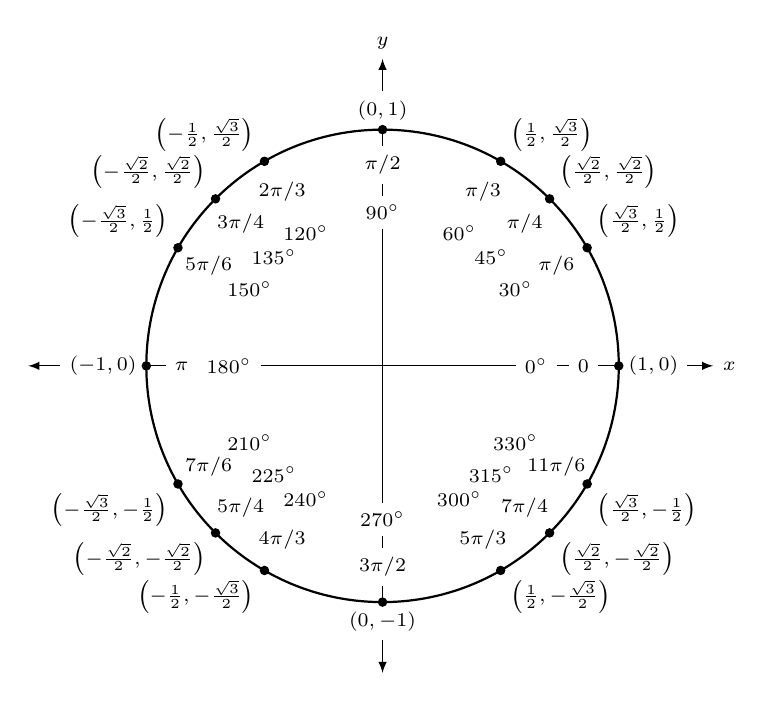
\begin{tikzpicture}[scale=3]
\draw [<->,>=latex] (-1.5,0) -- (1.4,0) node [right] {\scriptsize $x$};
\draw [<->,>=latex] (0,-1.3) -- (0,1.3) node [above] {\scriptsize $y$};
\foreach \x / \y / \z / \w / \v in {
								0/0/{1,0}/right/white,
								30/{\pi/6}/{\frac{\sqrt{3}}2,\frac 12}/above right/none,%
								45/{\pi/4}/{\frac{\sqrt{2}}2,\frac{\sqrt{2}}2}/above right/none,
								60/{\pi/3}/{\frac{1}2,\frac{\sqrt{3}}2}/{above right}/none,
								90/ {\pi/2}/{0,1}/above/white,%
								120/{2\pi/3}/{-\frac{1}2,\frac{\sqrt{3}}2}/above left/none, 
								135/{3\pi/4}/{-\frac{\sqrt{2}}2,\frac{\sqrt{2}}2}/above left/none, 
								150/ {5\pi/6}/{-\frac{\sqrt{3}}2,\frac{1}2}/above left/none,%
								180/ {\pi}/{-1,0}/left/white, 
								210/{7\pi/6}/{-\frac{\sqrt{3}}2,-\frac{1}2}/below left/none, 
								225/{5\pi/4}/{-\frac{\sqrt{2}}2,-\frac{\sqrt{2}}2}/below left/none, 
								240/{4\pi/3}/{-\frac{1}2,-\frac{\sqrt{3}}2}/below left/none,
								270/{3\pi/2}/{0,-1}/below/white, 
								300/{5\pi/3}/{\frac{1}2,-\frac{\sqrt{3}}2}/below right/none, 
								315/{7\pi/4}/{\frac{\sqrt{2}}2,-\frac{\sqrt{2}}2}/below right/none, 
								330/{11\pi/6}/{\frac{\sqrt{3}}2,-\frac{1}2}/below right/none%
										}
	{%
		\draw (\x:.65cm) node [fill=\v] {\scriptsize \x$^\circ$};
		\draw (\x:.85cm) node [fill=\v] {\scriptsize $\y$};
		\draw (\x:1cm) node [\w,fill=\v] {\scriptsize $\left(\z\right)$};
		\draw [fill=black] (\x:1) circle (.5pt);
	}

\draw [thick] (0,0) circle (1);

\end{tikzpicture}
\end{minipage}
%
\begin{minipage}[t]{.45\linewidth}
\noindent\textbf{\large Definitions of the Trigonometric Functions}\\

\noindent%
\small
%\begin{minipage}[t]{.48\linewidth}
\textbf{\normalsize Unit Circle Definition}

\noindent
%
\begin{minipage}{.56\linewidth}
\centering
\vskip 0in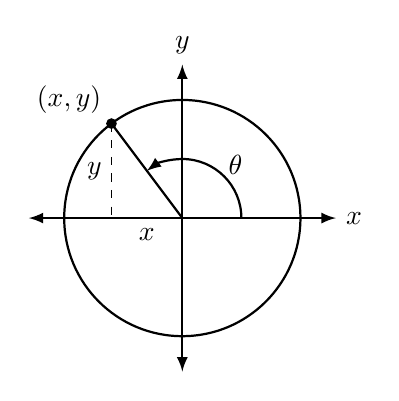
\begin{tikzpicture}[>=latex,scale=1.5,thick]
\draw [<->](-1.3,0)--(1.3,0) node [right] {$x$};
\draw [<->] (0,-1.3) -- (0,1.3) node [above] {$y$};
\draw (0,0) circle (1);
\draw [fill= black] (-.6,.8) circle (1pt);
\draw (0,0) -- (-.6,.8) node [above left] {$(x,y)$};
\draw [->] (.5,0) arc (0:127:.5);
\draw [dashed,thin] (-.6,.8) -- (-.6,0) node [pos=.5,left] {$y$};
\draw (-.3,0) node [below] {$x$};
\draw (.45,.45) node {$\theta$};
\end{tikzpicture}
\end{minipage}
\begin{minipage}{.4\linewidth}
\vskip 0in \small
\begin{tabular}{cc}
$\sin \theta = y$ & $\cos \theta = x$ \\
\\
$\ds\csc \theta = \frac1y$&$\ds\sec \theta = \frac1x$ \\
\\
$\myrule\ds\tan \theta = \frac yx$ & $\ds\cot \theta = \frac xy$
\end{tabular}
\end{minipage}
%\rule[-50pt]{.5pt}{100pt}
%
%\end{minipage}\hskip .02\linewidth
%\begin{minipage}[t]{.5\linewidth}
%Right Triangle Definition\\
%
%\noindent
\noindent\textbf{\normalsize Right Triangle Definition}

\begin{minipage}{.56\linewidth}
\centering
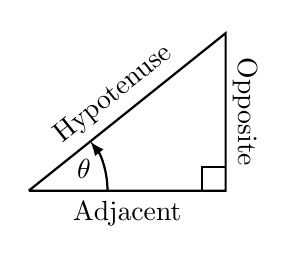
\begin{tikzpicture}[thick]
\draw (0,0) -- (2.5,0) node [below,pos=.5] {Adjacent} -- (2.5,2) node [pos=.5,rotate=-90,shift={(0pt,7pt)}] {Opposite} -- (0,0) node [pos=.5,above,rotate=38.7] {Hypotenuse} node [shift={(20pt,8pt)}] {$\theta$};
\draw[->,>=latex] (1,0) arc (0:38.7:1);
\draw (2.2,0) -- (2.2,.3) -- (2.5,.3);
\end{tikzpicture}
\end{minipage}
\begin{minipage}{.4\linewidth}
\vskip 0in \small
\begin{tabular}{cc}
$\ds\sin \theta = \frac{\text{O}}{\text{H}}$ & $\ds\csc \theta = \frac{\text{H}}{\text{O}}$ \\
\\
$\ds\cos \theta = \frac{\text{A}}{\text{H}}$ & $\ds\sec \theta = \frac{\text{H}}{\text{A}}$ \\
\\
$\ds\tan \theta = \frac{\text{O}}{\text{A}}$ & $\ds\cot \theta = \frac{\text{A}}{\text{O}}$ \\
\end{tabular}
\end{minipage}
\end{minipage}
\normalsize

\vskip \baselineskip
\noindent\textbf{\large Common Trigonometric Identities}\\
\vskip \baselineskip
\noindent%
\begin{minipage}[t]{.25\linewidth}
	\noindent\textbf{Pythagorean Identities}\vskip 5pt

	\noindent$\ds \sin ^2x+\cos ^2x= 1$\vskip 5pt

	\noindent$\ds \tan^2x+ 1 = \sec^2 x$\vskip 5pt

	\noindent$\ds 1 + \cot^2x=\csc^2 x$\vskip 5pt
\end{minipage}
\begin{minipage}[t]{.45\linewidth}
	\textbf{Cofunction Identities}\vskip 5pt
	\begin{minipage}[t]{.45\linewidth}
		$\ds \sin\left(\frac{\pi}{2}-x\right) = \cos x$\vskip 5pt
		$\ds \cos\left(\frac{\pi}{2}-x\right) = \sin x$\vskip 5pt
		$\ds \tan\left(\frac{\pi}{2}-x\right) = \cot x$\vskip 5pt
	\end{minipage}
	\begin{minipage}[t]{.45\linewidth}
		$\ds \csc\left(\frac{\pi}{2}-x\right) = \sec x$\vskip 5pt
		$\ds \sec\left(\frac{\pi}{2}-x\right) = \csc x$\vskip 5pt
		$\ds \cot\left(\frac{\pi}{2}-x\right) = \tan x$\vskip 5pt
	\end{minipage}
\end{minipage}
\begin{minipage}[t]{.25\linewidth}
	\textbf{Double Angle Formulas}\vskip 5pt
	$\sin 2x = 2\sin x\cos x$ \vskip 5pt
	$\cos 2x = \cos^2x - \sin^2 x$\vskip 5pt
	$\phantom{\cos 2x}= 2\cos^2x-1$\vskip 5pt
	$\phantom{\cos 2x}= 1-2\sin^2x$\vskip 5pt
	$\ds\tan 2x = \frac{2\tan x}{1-\tan^2 x}$
\end{minipage}

\vskip \baselineskip

\noindent%
\begin{minipage}[t]{.44\linewidth}
\textbf{Sum to Product Formulas}\vskip 5pt
$\ds \sin x+\sin y = 2\sin \left(\frac{x+y}2\right)\cos\left(\frac{x-y}2\right)$\vskip 5pt
$\ds \sin x-\sin y = 2\sin \left(\frac{x-y}2\right)\cos\left(\frac{x+y}2\right)$\vskip 5pt
$\ds \cos x+\cos y = 2\cos \left(\frac{x+y}2\right)\cos\left(\frac{x-y}2\right)$\vskip 5pt
$\ds \cos x-\cos y = -2\sin \left(\frac{x+y}2\right)\sin\left(\frac{x-y}2\right)$\vskip 5pt
\end{minipage}
\begin{minipage}[t]{.3\linewidth}
\textbf{Power--Reducing Formulas}\vskip 5pt
$\ds \sin^2 x = \frac{1-\cos 2x}{2}$\vskip 5pt
$\ds \cos^2 x = \frac{1+\cos 2x}{2}$\vskip 5pt
$\ds \tan^2x = \frac{1-\cos 2x}{1+\cos 2x}$
\end{minipage}
\begin{minipage}[t]{.25\linewidth}
\textbf{Even/Odd Identities}\vskip 5pt
$\sin(-x) = -\sin x$\vskip 5pt
$\cos (-x) = \cos x$\vskip 5pt
$\tan (-x) = -\tan x$\vskip 5pt
$\csc(-x) = -\csc x$\vskip 5pt
$\sec (-x) = \sec x$\vskip 5pt
$\cot (-x) = -\cot x$\vskip 5pt
\end{minipage}

\vskip \baselineskip

\noindent
\begin{minipage}[t]{.45\linewidth}
\textbf{Product to Sum Formulas}\vskip 5pt
$\ds \sin x\sin y = \frac12 \big(\cos(x-y) - \cos (x+y)\big)$\vskip 5pt
$\ds \cos x\cos y = \frac12\big(\cos (x-y) +\cos (x+y)\big)$\vskip 5pt
$\ds \sin x\cos y = \frac12 \big(\sin(x+y) + \sin (x-y)\big)$\vskip 5pt
\end{minipage}
\begin{minipage}[t]{.45\linewidth}
\textbf{Angle Sum/Difference Formulas}\vskip 5pt
$\sin (x\pm y) = \sin x\cos y \pm \cos x\sin y$\vskip 5pt
$\cos (x\pm y) = \cos x\cos y \mp \sin x\sin y$\vskip 5pt
$\ds \tan (x\pm y) = \frac{\tan x\pm \tan y}{1\mp \tan x\tan y}$
\end{minipage}

\clearpage

\noindent\textbf{\large Areas and Volumes}
\vskip \baselineskip
%\begin{tabular}{cc}
\noindent%
%
\begin{minipage}[t]{225pt}
		\begin{minipage}[t]{100pt}
		\noindent\textbf{Triangles}\vskip 5pt
		$h=a\sin \theta$\vskip 5pt
		Area = $\frac12bh$\vskip 5pt
		Law of Cosines:%\vskip 4pt
		
		$c^2=a^2+b^2-2ab\cos \theta$\vskip 5pt
		\end{minipage}
		\begin{minipage}[t]{115pt}
			\centering
			\vskip 0pt
			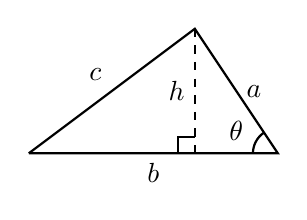
\begin{tikzpicture}[x=30pt,y=30pt,thick]
			\draw (0,0) -- node [below,pos=.5]  { $b$} (3,0) node [shift={(-15pt,8pt)}] {$\theta$} -- node [pos=.5,right] { $a$} (2,1.5) -- node [pos=.5,above left] { $c$} (0,0);
			\draw (2.7,0) arc (180:125:.3);
			\draw [dashed] (2,1.5) -- (2,0) node [pos=.5,left] {$h$};
			\draw (2,.2) -- (1.8,.2) -- (1.8,0);
			\end{tikzpicture}
		\end{minipage}
\end{minipage}
%
\begin{minipage}[t]{225pt}
	\begin{minipage}[t]{100pt}
		\noindent\textbf{Right Circular Cone}\vskip 5pt
		Volume = $\frac 13 \pi r^2h$ \vskip 5pt
		Surface Area =\vskip 3pt		
		 $\pi r\sqrt{r^2+h^2} +\pi r^2$
		\end{minipage}
		\begin{minipage}[t]{115pt}
			\centering
			\vskip 0pt
			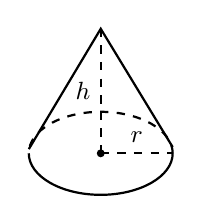
\begin{tikzpicture}[x=13pt,y=15pt,thick]
			\begin{scope}[xscale=2]
			\draw (-1,0) arc (-180:0:1);
			\draw [dashed] (1,0) arc (0:180:1);
			\draw (-1,.1) -- (0,3) -- (1,.15);
			\draw [dashed] (0,3) -- node [pos=.5,left] {\small $h$} (0,0);
			\draw [dashed] (0,0) -- (1,0) node [pos=.5,above] {\small $r$};
			\end{scope}
			\draw [fill=black] (0,0) circle (1pt);
			\end{tikzpicture}
		\end{minipage}
\end{minipage}

\vskip 2\baselineskip
\noindent%
\begin{minipage}[t]{225pt}
		\begin{minipage}[t]{100pt}
		\noindent\textbf{Parallelograms}\vskip 5pt
		Area = $bh$
		\end{minipage}
		\begin{minipage}[t]{115pt}
			\centering
			\vskip 0pt
			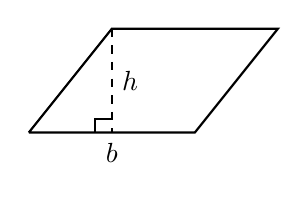
\begin{tikzpicture}[x=30pt,y=25pt,thick]
			\draw (0,0) -- node [below,pos=.5]  { $b$} (2,0) -- (3,1.5) -- (1,1.5) -- (0,0);
			\draw [dashed] (1,1.5) -- (1,0) node [pos=.5,right] {$h$};
			\draw (.8,0) -- (.8,.2) -- (1,.2);
			\end{tikzpicture}
		\end{minipage}
\end{minipage}
\begin{minipage}[t]{225pt}
\begin{minipage}[t]{100pt}
		\noindent\textbf{Right Circular Cylinder}\vskip 5pt
		Volume = $\pi r^2h$ \vskip 5pt
		Surface Area =\vskip 3pt		
		 $2\pi rh  +2\pi r^2$
		\end{minipage}
		\begin{minipage}[t]{115pt}
			\centering
			\vskip 0pt
			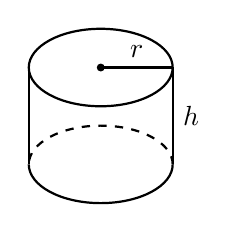
\begin{tikzpicture}[x=13pt,y=14pt,thick]
			\begin{scope}[xscale=2]
			\draw (-1,0) arc (-180:0:1);
			\draw [dashed] (1,0) arc (0:180:1);
			\draw (0,2.5) circle (1);
			\draw (-1,0) -- (-1,2.5) (1,0)-- (1,2.5) node [right,pos=.5] {$h$};
			\draw (0,2.5) -- (1,2.5) node [above,pos=.5] {$r$};
			\end{scope}
			\draw [fill=black] (0,2.5) circle (1pt);
			\end{tikzpicture}
		\end{minipage}

		
\end{minipage}

\vskip 2\baselineskip
\noindent%
\begin{minipage}[t]{225pt}
		\begin{minipage}[t]{100pt}
		\noindent\textbf{Trapezoids}\vskip 5pt
		Area = $\frac12(a+b)h$
		\end{minipage}
		\begin{minipage}[t]{115pt}
			\centering
			\vskip 0pt
			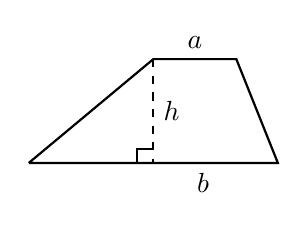
\begin{tikzpicture}[x=30pt,y=25pt,thick]
			\draw (0,0) -- node [below,pos=.7]  { $b$} (3,0) -- (2.5,1.5) -- node [above,pos=.5] {$a$} (1.5,1.5) -- (0,0);
			\draw [dashed] (1.5,1.5) -- (1.5,0) node [pos=.5,right] {$h$};
			\draw (1.3,0) -- (1.3,.2) -- (1.5,.2);
			\end{tikzpicture}
		\end{minipage}
\end{minipage}
\begin{minipage}[t]{225pt}
\begin{minipage}[t]{100pt}
		\noindent\textbf{Sphere}\vskip 5pt
		Volume = $\frac43\pi r^3$ \vskip 5pt
		Surface Area =$4\pi r^2$
		\end{minipage}
		\begin{minipage}[t]{115pt}
			\centering
			\vskip 0pt
			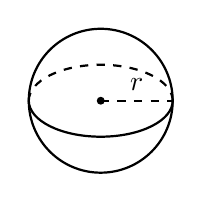
\begin{tikzpicture}[x=13pt,y=13pt,thick]
			\begin{scope}[xscale=2]
			\draw (-1,0) arc (-180:0:1);
			\draw [dashed] (1,0) arc (0:180:1);
			\end{scope}
			\draw (0,0) circle (2);
			\draw [dashed] (0,0) -- (2,0) node [pos=.5,above] {$r$};
			\draw [fill=black] (0,0) circle (1pt);
			\end{tikzpicture}
		\end{minipage}
\end{minipage}

\vskip 2\baselineskip
\noindent%
\begin{minipage}[t]{225pt}
		\begin{minipage}[t]{100pt}
		\noindent\textbf{Circles}\vskip 5pt
		Area = $\pi r^2$\vskip 5pt
		Circumference = $2\pi r$
		\end{minipage}
		\begin{minipage}[t]{115pt}
			\centering
			\vskip 0pt
			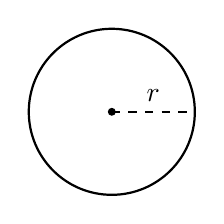
\begin{tikzpicture}[x=30pt,y=30pt,thick]
			\draw (0,0) circle (1);
			\draw [dashed] (0,0) -- (1,0) node [pos=.5,above] {$r$};
			\draw [fill=black] (0,0) circle (1pt);
			\end{tikzpicture}
		\end{minipage}
\end{minipage}
\begin{minipage}[t]{225pt}
\begin{minipage}[t]{100pt}
		\noindent\textbf{General Cone}\vskip 5pt
		Area of Base = $A$\vskip 5pt
		Volume = $\frac13Ah$ \vskip 5pt
		\end{minipage}
		\begin{minipage}[t]{115pt}
			\centering
			\vskip 0pt
			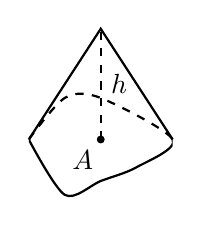
\begin{tikzpicture}[x=13pt,y=10pt,thick]
			\begin{scope}
			\clip (0,0) rectangle (4,-2.5);
			\draw [smooth] plot coordinates {(0,0) (1,1.5) (2,1.5) (4,0) (3,-1) (2,-1.5) (1,-2) (0,0)};
			\end{scope}
			\begin{scope}
			\clip (0,0) rectangle (4,2.5);
			\draw [smooth,dashed] plot coordinates {(0,0) (1,1.5) (2,1.5) (4,0) (3,-1) (2,-1.5) (1,-2) (0,0)};
			\end{scope}
			\draw (0,0) -- (2,4)--(4,0);
			\draw [dashed] (2,0)--(2,4) node [pos=.5,right] {$h$}; 
			\draw [fill=black](2,0) circle (1pt);
			\draw (1.5,-.75) node {$A$};
			\end{tikzpicture}
		\end{minipage}
\end{minipage}

\vskip 2\baselineskip
\noindent%
\begin{minipage}[t]{225pt}
		\begin{minipage}[t]{100pt}
		\noindent\textbf{Sectors of Circles}\vskip 5pt
		$\theta$ in radians \vskip 5pt
		Area = $\frac12\theta r^2$\vskip 5pt
		$s=r\theta$
		\end{minipage}
		\begin{minipage}[t]{115pt}
			\centering
			\vskip 0pt
			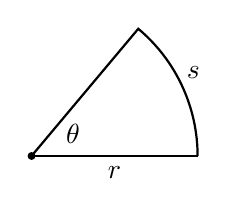
\begin{tikzpicture}[x=30pt,y=30pt,thick]
			\draw (2,0) arc (0:50:2) -- (0,0);
			\draw [] (0,0) -- (2,0) node [pos=.5,below] {$r$};
			\draw [fill=black] (0,0) circle (1pt);
			\draw (1.95,1.0) node {$s$};
			\draw (0,0) node [shift={(15pt,8pt)}] {$\theta$};
			\end{tikzpicture}
		\end{minipage}
\end{minipage}
\begin{minipage}[t]{225pt}
\begin{minipage}[t]{100pt}
		\noindent\textbf{General Right Cylinder}\vskip 5pt
		Area of Base = $A$\vskip 5pt
		Volume = $Ah$ \vskip 5pt
		\end{minipage}
		\begin{minipage}[t]{115pt}
			\centering
			\vskip 0pt
			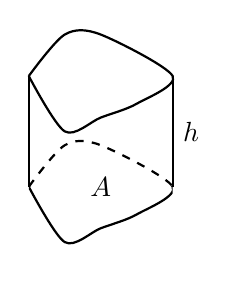
\begin{tikzpicture}[x=13pt,y=10pt,thick]
			\begin{scope}
			\clip (0,0) rectangle (4,-2.5);
			\draw [smooth] plot coordinates {(0,0) (1,1.5) (2,1.5) (4,0) (3,-1) (2,-1.5) (1,-2) (0,0)};
			\end{scope}
			\begin{scope}
			\clip (0,0) rectangle (4,2.5);
			\draw [smooth,dashed] plot coordinates {(0,0) (1,1.5) (2,1.5) (4,0) (3,-1) (2,-1.5) (1,-2) (0,0)};
			\end{scope}
			\begin{scope}[shift={(0,4)}]
			\draw [smooth] plot coordinates {(0,0) (1,1.5) (2,1.5) (4,0) (3,-1) (2,-1.5) (1,-2) (0,0)};
			\end{scope}
			\draw (0,0) -- (0,4) (4,0) -- (4,4) node [pos=.5,right] {$h$};
			\draw (2,0) node {$A$};
			\end{tikzpicture}
		\end{minipage}
\end{minipage}

\clearpage

\noindent\textbf{\Large Algebra}\vskip 2\baselineskip

\noindent \textbf{\large Factors and Zeros of Polynomials}\\
Let $p(x) = a_n x^n + a_{n-1} x^{n-1} + \cdots + a_1 x + a_0$ be a polynomial.  If $p(a)=0$, then $a$ is a $zero$ of the polynomial and a solution
of the equation $p(x)=0$.  Furthermore, $(x-a)$ is a $factor$ of the polynomial.
\vskip\baselineskip

\noindent \textbf{\large Fundamental Theorem of Algebra}\\
An $n$th degree polynomial has $n$ (not necessarily distinct) zeros.  Although all of these zeros may be imaginary, a real polynomial of odd degree
must have at least one real zero.\\
\vskip\baselineskip

\noindent \textbf{\large Quadratic Formula}\\
If $p(x) = ax^2 + bx + c$, and $0 \le b^2 - 4ac$, then the real zeros of $p$ are $x=(-b\pm \sqrt{b^2-4ac})/2a$\\
\vskip\baselineskip

\noindent \textbf{\large Special Factors}\\
$
\begin{array}{ll}
x^2 - a^2 = (x-a)(x+a) \qquad \qquad \qquad & x^3 - a^3 = (x-a)(x^2+ax+a^2)\\	
x^3 + a^3 = (x+a)(x^2-ax+a^2) \qquad \qquad \qquad & x^4 - a^4 = (x^2-a^2)(x^2+a^2)\\	
\end{array}
$

\noindent$\begin{array}{l}
(x+y)^n  =x^n + nx^{n-1}y+\frac{n(n-1)}{2!}x^{n-2}y^2+\cdots +nxy^{n-1}+y^n\\
(x-y)^n  =x^n - nx^{n-1}y+\frac{n(n-1)}{2!}x^{n-2}y^2-\cdots \pm nxy^{n-1}\mp y^n
\end{array}$\vskip \baselineskip


\noindent \textbf{\large Binomial Theorem}\\
$
\begin{array}{ll}
(x+y)^2 = x^2 + 2xy + y^2 \qquad & (x-y)^2 = x^2 -2xy +y^2\\
(x+y)^3 = x^3 + 3x^2y + 3xy^2 + y^3 \qquad  & (x-y)^3 = x^3 -3x^2y + 3xy^2 -y^3\\
(x+y)^4 = x^4 + 4x^3y + 6x^2y^2 + 4xy^3 + y^4 \qquad  & (x-y)^4 = x^4 - 4x^3y + 6x^2y^2 - 4xy^3 + y^4\\
\end{array}
$\vskip\baselineskip

\noindent \textbf{\large Rational Zero Theorem}\\
If $p(x) = a_n x^n + a_{n-1} x^{n-1} + \cdots + a_1 x + a_0$ has integer coefficients, then every $rational$ $zero$ of $p$ is of the form
$x=r/s$, where $r$ is a factor of $a_0$ and $s$ is a factor of $a_n$.\\
\vskip\baselineskip

\noindent \textbf{\large Factoring by Grouping}\\
$ac x^3 + adx^2 + bcx + bd = ax^2(cx+d)+b(cx+d)=(ax^2+b)(cx+d)$\\
\vskip\baselineskip

\noindent \textbf{\large Arithmetic Operations}\\
$
\begin{array}{lll}
ab+ac=a(b+c) \qquad \qquad & \displaystyle \frac{a}{b}+\frac{c}{d} = \frac{ad+bc}{bd} \qquad \qquad & \displaystyle \frac{a+b}{c} = \frac{a}{c} + \frac{b}{c}\\	\\
\displaystyle\frac{\left(\displaystyle\frac{a}{b}\right)}{\left(\displaystyle\frac{c}{d}\right)}=\left(\frac{a}{b}\right)\left(\frac{d}{c}\right)=\frac{ad}{bc} 
&\displaystyle \frac{\left(\displaystyle\frac{a}{b}\right)}{c} =\displaystyle \frac{a}{bc}
&\displaystyle \frac{a}{\left(\displaystyle\frac{b}{c}\right)} =\displaystyle \frac{ac}{b}\\ \\
a\left(\displaystyle\frac{b}{c}\right)= \displaystyle \frac{ab}{c}&\displaystyle\frac{a-b}{c-d}=\frac{b-a}{d-c}&\displaystyle\frac{ab+ac}{a}=b+c\\
\end{array}
$\vskip \baselineskip

\noindent \textbf{\large Exponents and Radicals}\\[5pt]
$
\begin{array}{llllll}
a^0=1, \; \; a \ne 0 \quad & (ab)^x=a^xb^x \quad & a^xa^y = a^{x+y}\quad  & \sqrt{a}=a^{1/2}   &\displaystyle \frac{a^x}{a^y}=a^{x-y}  &\sqrt[n]{a}=a^{1/n}\\[15pt]
\left(\displaystyle\frac{a}{b}\right)^x=\displaystyle\frac{a^x}{b^x} &\sqrt[n]{a^m}=a^{m/n} & a^{-x}=\displaystyle\frac{1}{a^x} & \sqrt[n]{ab}=\sqrt[n]{a}\sqrt[n]{b} \quad &
(a^x)^y=a^{xy} \quad& \displaystyle\sqrt[n]{\frac{a}{b}}=\frac{\sqrt[n]{a}}{\sqrt[n]{b}}
\end{array}
$

\clearpage
\noindent \textbf{\Large Additional Formulas}
\vskip 3\baselineskip

\noindent\textbf{\large Summation Formulas:}\\

\noindent\begin{tabular}{ll}
$\ds \sum^n_{i=1}{c} = cn$ \hskip 100pt\ & $\ds\sum^n_{i=1}{i} = \frac{n(n+1)}{2}$\\
$\ds\sum^n_{i=1}{i\hskip1pt^2} = \frac{n(n+1)(2n+1)}{6}$ & $\ds\sum^n_{i=1}{i\hskip1pt^3}= \left(\frac{n(n+1)}{2}\right)^2$\\
\end{tabular}\\[5pt]
\vskip2\baselineskip

\noindent\textbf{\large Trapezoidal Rule:}\\

\noindent$\ds%\begin{eqnarray*}
\int_a^b{f(x)}\ dx  \approx \frac{\Delta x}{2}\big[f(x_1)+2f(x_2) + 2f(x_3) + \cdots + 2f(x_{n}) + f(x_{n+1})\big]$ \\[5pt]
%\end{eqnarray*}
with  $\displaystyle \text{Error} \leq \frac{(b-a)^3}{12n^2}\big[ \max \big| \ifthenelse{\boolean{xetex}}{f\,''(x)}{f''(x)} \big|\big]$
\vskip2\baselineskip

\noindent\textbf{\large Simpson's Rule:}\\

\noindent$\ds\int_a^b{f(x)}\ dx  \approx  \frac{\Delta x}{3}\big[f(x_1)+4f(x_2) + 2f(x_3) + 4f(x_4) + \cdots + 2f(x_{n-1}) + 4f(x_{n}) + f(x_{n+1})\big] 
$\\[5pt]
with $\displaystyle \text{Error} \leq \frac{(b-a)^5}{180n^4}\big[ \max \big| \ifthenelse{\boolean{xetex}}{f\,^{(4)}(x)}{f^{(4)}(x)} \big|\big]
$
\vskip 2\baselineskip

\noindent\begin{minipage}[t]{.5\linewidth}
\textbf{\large Arc Length:}\\[5pt]
$\displaystyle
L = \int_a^b{\sqrt{1+ f\,'(x)^2}}\phantom{a}dx  
$\\[5pt]

%$\displaystyle
%s = \int_c^d{\sqrt{1+ (g'(y))^2}}\phantom{a}dy 
%$
\end{minipage}
\begin{minipage}[t]{.49\linewidth}
\textbf{\large Surface of Revolution:}
\\[5pt]
$\displaystyle
S = 2\pi \int_a^b{f(x) \sqrt{1+ f\,'(x)^2}}\phantom{a}dx  
$\\[3pt]
{\small (where $f(x)\geq 0$)}\\[5pt]

$\displaystyle
S = 2\pi \int_a^b{x \sqrt{1+ f\,'(x)^2}}\phantom{a}dx 
$\\[3pt]
{\small (where $a,b \geq 0$)}
\end{minipage}
\vskip2\baselineskip

\noindent\begin{minipage}[t]{.49\linewidth}
\textbf{\large Work Done by a Variable Force:}\\[5pt]
$\displaystyle
W = \int_a^b{F(x)}\phantom{a}dx  
$
\end{minipage}
\begin{minipage}[t]{.5\linewidth}
\textbf{\large Force Exerted by a Fluid:}\\[5pt]
$\displaystyle
F = \int_a^b{w\,d(y)\,\ell(y)}\phantom{a}dy  
$
\end{minipage}
\vskip2\baselineskip

\noindent\textbf{\large Taylor Series Expansion for $f(x)$:}\\[5pt]
\noindent$\displaystyle p_n(x) = f(c) + f\,'(c)(x-c) + \frac{f\,''(c)}{2!}(x-c)^2 + \frac{f\,'''(c)}{3!}(x-c)^3 + \cdots + \frac{f\,^{(n)}(c)}{n!}(x-c)^n + \cdots$
\vskip2\baselineskip

\noindent\textbf{\large Maclaurin Series Expansion for $f(x)$, where $c=0$:}\\[5pt]
\noindent$\displaystyle p_n(x) = f(0) + f\,'(0)x + \frac{f\,''(0)}{2!}x^2 + \frac{f\,'''(0)}{3!}x^3 + \cdots + \frac{f\,^{(n)}(0)}{n!}x^n+\cdots$

\clearpage

\noindent\textbf{\large Summary of Tests for Series:}\\[5pt]

\noindent\begin{tabular}{|c|c|c|c|c|}
\hline
Test & Series & \rule[-15pt]{0pt}{33pt}\parbox{1in}{\centering Condition(s) of Convergence} & \parbox{1in}{\centering Condition(s) of Divergence} &   Comment \\ \hline
$n$th-Term & \rule[-15pt]{0pt}{33pt}$\displaystyle{\sum^\infty_{n=1}{a_n}}$ &  & $\displaystyle{\lim_{n \to \infty} a_n \neq 0}$ & \parbox{1.5in}{This test cannot be used to show convergence.}\\ \hline

Geometric Series & \rule[-15pt]{0pt}{33pt}$\displaystyle{\sum^\infty_{n=0}{r^n}}$ & $ \left| r \right| < 1$ & $\left| r \right| \geq 1$ &  $\displaystyle{\text{Sum} = \frac{1}{1-r}}$ \\ \hline

Telescoping Series &\rule[-15pt]{0pt}{33pt} $\displaystyle{\sum^\infty_{n=1}{(b_n-b_{n+a})}}$ & $\displaystyle{\lim_{n \to \infty} b_n = L}$ & & $\displaystyle\text{Sum}= \left(\sum^a_{n=1}b_n\right) -L$ \\ \hline

$p$-Series & \rule[-15pt]{0pt}{33pt}$\displaystyle{\sum^\infty_{n=1}{\frac{1}{(an+b)^p}}}$ & $p>1$ & $p\leq 1$ & \\ \hline

Integral Test & \rule[-20pt]{0pt}{40pt}$\displaystyle{\sum^\infty_{n=0}{a_n}}$ & \rule[-15pt]{0pt}{40pt}\parbox{1in}{\centering$\displaystyle \int_1^\infty a(n)\ dn$\\[3pt] is convergent} & \parbox{1in}{\centering$\displaystyle \int_1^\infty a(n)\ dn$\\[3pt] is divergent} & \parbox{1.2in}{$a_n = a(n)$ must be continuous}\\ \hline

Direct Comparison & \rule[-30pt]{0pt}{65pt}$\displaystyle{\sum^\infty_{n=0}{a_n}}$ & \parbox{1in}{\centering$\displaystyle \sum_{n=0}^\infty b_n $\\[3pt] converges and \\[3pt] $0\leq a_n\leq b_n$}%
& \parbox{1in}{\centering$\displaystyle \sum_{n=0}^\infty b_n $\\[3pt] diverges and \\[3pt] $0\leq b_n\leq a_n$} & \\ \hline

Limit Comparison & \rule[-30pt]{0pt}{65pt}$\displaystyle{\sum^\infty_{n=0}{a_n}}$ & \parbox{1.3in}{\centering$\displaystyle \sum_{n=0}^\infty b_n $\\[3pt] converges and \\[3pt] $\displaystyle \lim_{n\to\infty} a_n/b_n  \geq 0$}%
& \parbox{1in}{\centering$\displaystyle \sum_{n=0}^\infty b_n $\\[3pt] diverges and \\[3pt] $\displaystyle \lim_{n\to\infty} a_n/b_n > 0$}  & \parbox{1.5in}{\centering Also diverges if\\[3pt] $\displaystyle \lim_{n\to\infty} a_n/b_n=\infty$}\\ \hline

Ratio Test & \rule[-30pt]{0pt}{65pt}$\displaystyle{\sum^\infty_{n=0}{a_n}}$ &%
 \parbox{1.3in}{\centering$\displaystyle \lim_{n\to\infty} \frac{a_{n+1}}{a_n}  < 1$}%
& \parbox{1.3in}{\centering$\displaystyle \lim_{n\to\infty} \frac{a_{n+1}}{a_n} > 1$} & 
\parbox{1.5in}{\centering $\{a_n\}$ must be positive\\[3pt] Also diverges if\\[3pt] $\displaystyle \lim_{n\to\infty} a_{n+1}/a_n=\infty$}\\ \hline

Root Test & \rule[-30pt]{0pt}{65pt}$\displaystyle{\sum^\infty_{n=0}{a_n}}$ &%
 \parbox{1.3in}{\centering$\displaystyle \lim_{n\to\infty} \big(a_n\big)^{1/n}  < 1$}%
& \parbox{1.3in}{\centering$\displaystyle \lim_{n\to\infty} \big(a_n\big)^{1/n} > 1$} & 
\parbox{1.5in}{\centering $\{a_n\}$ must be positive\\[3pt] Also diverges if\\[3pt] $\displaystyle \lim_{n\to\infty} \big(a_n\big)^{1/n}=\infty$}\\ \hline

\end{tabular}


%\end{document}



\end{document}

